\documentclass[spanish,]{article}
\usepackage{lmodern}
\usepackage{amssymb,amsmath}
\usepackage{ifxetex,ifluatex}
\usepackage{fixltx2e} % provides \textsubscript
\ifnum 0\ifxetex 1\fi\ifluatex 1\fi=0 % if pdftex
  \usepackage[T1]{fontenc}
  \usepackage[utf8]{inputenc}
\else % if luatex or xelatex
  \ifxetex
    \usepackage{mathspec}
  \else
    \usepackage{fontspec}
  \fi
  \defaultfontfeatures{Ligatures=TeX,Scale=MatchLowercase}
\fi
% use upquote if available, for straight quotes in verbatim environments
\IfFileExists{upquote.sty}{\usepackage{upquote}}{}
% use microtype if available
\IfFileExists{microtype.sty}{%
\usepackage{microtype}
\UseMicrotypeSet[protrusion]{basicmath} % disable protrusion for tt fonts
}{}
\usepackage[margin=1in]{geometry}
\usepackage{hyperref}
\hypersetup{unicode=true,
            pdfauthor={Alejandro Campoy Nieves; Gema Correa Fernández; Luis Gallego Quero; Jonathan Martín Valera; Andrea Morales Garzón},
            pdfborder={0 0 0},
            breaklinks=true}
\urlstyle{same}  % don't use monospace font for urls
\ifnum 0\ifxetex 1\fi\ifluatex 1\fi=0 % if pdftex
  \usepackage[shorthands=off,main=spanish]{babel}
\else
  \usepackage{polyglossia}
  \setmainlanguage[]{spanish}
\fi
\usepackage{color}
\usepackage{fancyvrb}
\newcommand{\VerbBar}{|}
\newcommand{\VERB}{\Verb[commandchars=\\\{\}]}
\DefineVerbatimEnvironment{Highlighting}{Verbatim}{commandchars=\\\{\}}
% Add ',fontsize=\small' for more characters per line
\usepackage{framed}
\definecolor{shadecolor}{RGB}{248,248,248}
\newenvironment{Shaded}{\begin{snugshade}}{\end{snugshade}}
\newcommand{\KeywordTok}[1]{\textcolor[rgb]{0.13,0.29,0.53}{\textbf{#1}}}
\newcommand{\DataTypeTok}[1]{\textcolor[rgb]{0.13,0.29,0.53}{#1}}
\newcommand{\DecValTok}[1]{\textcolor[rgb]{0.00,0.00,0.81}{#1}}
\newcommand{\BaseNTok}[1]{\textcolor[rgb]{0.00,0.00,0.81}{#1}}
\newcommand{\FloatTok}[1]{\textcolor[rgb]{0.00,0.00,0.81}{#1}}
\newcommand{\ConstantTok}[1]{\textcolor[rgb]{0.00,0.00,0.00}{#1}}
\newcommand{\CharTok}[1]{\textcolor[rgb]{0.31,0.60,0.02}{#1}}
\newcommand{\SpecialCharTok}[1]{\textcolor[rgb]{0.00,0.00,0.00}{#1}}
\newcommand{\StringTok}[1]{\textcolor[rgb]{0.31,0.60,0.02}{#1}}
\newcommand{\VerbatimStringTok}[1]{\textcolor[rgb]{0.31,0.60,0.02}{#1}}
\newcommand{\SpecialStringTok}[1]{\textcolor[rgb]{0.31,0.60,0.02}{#1}}
\newcommand{\ImportTok}[1]{#1}
\newcommand{\CommentTok}[1]{\textcolor[rgb]{0.56,0.35,0.01}{\textit{#1}}}
\newcommand{\DocumentationTok}[1]{\textcolor[rgb]{0.56,0.35,0.01}{\textbf{\textit{#1}}}}
\newcommand{\AnnotationTok}[1]{\textcolor[rgb]{0.56,0.35,0.01}{\textbf{\textit{#1}}}}
\newcommand{\CommentVarTok}[1]{\textcolor[rgb]{0.56,0.35,0.01}{\textbf{\textit{#1}}}}
\newcommand{\OtherTok}[1]{\textcolor[rgb]{0.56,0.35,0.01}{#1}}
\newcommand{\FunctionTok}[1]{\textcolor[rgb]{0.00,0.00,0.00}{#1}}
\newcommand{\VariableTok}[1]{\textcolor[rgb]{0.00,0.00,0.00}{#1}}
\newcommand{\ControlFlowTok}[1]{\textcolor[rgb]{0.13,0.29,0.53}{\textbf{#1}}}
\newcommand{\OperatorTok}[1]{\textcolor[rgb]{0.81,0.36,0.00}{\textbf{#1}}}
\newcommand{\BuiltInTok}[1]{#1}
\newcommand{\ExtensionTok}[1]{#1}
\newcommand{\PreprocessorTok}[1]{\textcolor[rgb]{0.56,0.35,0.01}{\textit{#1}}}
\newcommand{\AttributeTok}[1]{\textcolor[rgb]{0.77,0.63,0.00}{#1}}
\newcommand{\RegionMarkerTok}[1]{#1}
\newcommand{\InformationTok}[1]{\textcolor[rgb]{0.56,0.35,0.01}{\textbf{\textit{#1}}}}
\newcommand{\WarningTok}[1]{\textcolor[rgb]{0.56,0.35,0.01}{\textbf{\textit{#1}}}}
\newcommand{\AlertTok}[1]{\textcolor[rgb]{0.94,0.16,0.16}{#1}}
\newcommand{\ErrorTok}[1]{\textcolor[rgb]{0.64,0.00,0.00}{\textbf{#1}}}
\newcommand{\NormalTok}[1]{#1}
\usepackage{graphicx,grffile}
\makeatletter
\def\maxwidth{\ifdim\Gin@nat@width>\linewidth\linewidth\else\Gin@nat@width\fi}
\def\maxheight{\ifdim\Gin@nat@height>\textheight\textheight\else\Gin@nat@height\fi}
\makeatother
% Scale images if necessary, so that they will not overflow the page
% margins by default, and it is still possible to overwrite the defaults
% using explicit options in \includegraphics[width, height, ...]{}
\setkeys{Gin}{width=\maxwidth,height=\maxheight,keepaspectratio}
\IfFileExists{parskip.sty}{%
\usepackage{parskip}
}{% else
\setlength{\parindent}{0pt}
\setlength{\parskip}{6pt plus 2pt minus 1pt}
}
\setlength{\emergencystretch}{3em}  % prevent overfull lines
\providecommand{\tightlist}{%
  \setlength{\itemsep}{0pt}\setlength{\parskip}{0pt}}
\setcounter{secnumdepth}{0}
% Redefines (sub)paragraphs to behave more like sections
\ifx\paragraph\undefined\else
\let\oldparagraph\paragraph
\renewcommand{\paragraph}[1]{\oldparagraph{#1}\mbox{}}
\fi
\ifx\subparagraph\undefined\else
\let\oldsubparagraph\subparagraph
\renewcommand{\subparagraph}[1]{\oldsubparagraph{#1}\mbox{}}
\fi

%%% Use protect on footnotes to avoid problems with footnotes in titles
\let\rmarkdownfootnote\footnote%
\def\footnote{\protect\rmarkdownfootnote}

%%% Change title format to be more compact
\usepackage{titling}

% Create subtitle command for use in maketitle
\newcommand{\subtitle}[1]{
  \posttitle{
    \begin{center}\large#1\end{center}
    }
}

\setlength{\droptitle}{-2em}

  \title{}
    \pretitle{\vspace{\droptitle}}
  \posttitle{}
    \author{Alejandro Campoy Nieves \\ Gema Correa Fernández \\ Luis Gallego Quero \\ Jonathan Martín Valera \\ Andrea Morales Garzón}
    \preauthor{\centering\large\emph}
  \postauthor{\par}
      \predate{\centering\large\emph}
  \postdate{\par}
    \date{14 de noviembre de 2018}

\usepackage{fancyhdr}
\fancyfoot[CO,CE]{My footer}
\usepackage{color}
\usepackage{colortbl}
\usepackage{multicol}
\usepackage{multirow}

\begin{document}

\thispagestyle{empty}

\begin{center} \huge \textbf{Tratamiento Inteligente de datos} \end{center}

\vspace{0.3cm}

\begin{center} \huge \textbf{(TID)} \end{center}

\vspace{1.7cm}

\begin{center} \Large \textbf{\textsc{Prácticas de la asignatura}} \end{center}

\vspace{0.2cm}

\begin{center} \large \textbf{2018-2019} \end{center}

\vspace{2.5cm}

\textbf{\large En colaboración con:} \vspace{0.2cm}

\begin{figure}[h]
    \centering
    
\includegraphics[width=0.7\textwidth]{imagenes/logoUGR.jpg}
    \label{imagen2}
\end{figure}

\vspace{2.5cm}

\hspace{8.5cm}{\large \textbf{Participantes}}

\vspace{0.25cm}

\hspace{8.5cm}{Alejandro Campoy Nieves:  \href{mailto:alejandroac79@correo.ugr.es}{\textcolor{blue}{\underline{alejandroac79@correo.ugr.es}}}}

\vspace{0.15cm}

\hspace{8.5cm}{Gema Correa Fernández:  \href{mailto:gecorrea@correo.ugr.es}{\textcolor{blue}{\underline{gecorrea@correo.ugr.es}}} }

\vspace{0.15cm}

\hspace{8.5cm}{Luis Gallego Quero:  \href{mailto:lgaq94@correo.ugr.es}{\textcolor{blue}{\underline{lgaq94@correo.ugr.es}}} }

\vspace{0.15cm}

\hspace{8.5cm}{Jonathan Martín Valera:  \href{mailto:jmv742@correo.ugr.es}{\textcolor{blue}{\underline{jmv742@correo.ugr.es}}} }

\vspace{0.15cm}

\hspace{8.5cm}{Andrea Morales Garzón:  \href{mailto:andreamgmg@correo.ugr.es}{\textcolor{blue}{\underline{andreamgmg@correo.ugr.es}}} }

\vspace{0.15cm}

\newpage

\thispagestyle{empty} \tableofcontents
\newpage

\thispagestyle{empty} \listoffigures
\newpage

\thispagestyle{empty} \listoftables
\newpage

\pagestyle{fancy} \fancyhf{}
\lhead{Proyecto: Técnicas aplicadas para análisis inteligente de datos}
\rhead{\thepage} \setcounter{page}{1}

\section{Descripción de los paquetes
necesarios}\label{descripcion-de-los-paquetes-necesarios}

A continuación, se describen los paquetes necesarios para el desarollo
del proyecto:

\begin{itemize}
\item
  \href{https://cran.r-project.org/web/packages/arules/arules.pdf}{\texttt{arules}}
  : Paquete que proporciona la infraestructura para representar,
  manipular y analizar datos y patrones de transacción (conjuntos de
  elementos frecuentes y reglas de asociación). Se puede instalar usando
  : \emph{install.packages(``arules'')}.
\item
  \href{https://cran.r-project.org/web/packages/arulesViz/arulesViz.pdf}{\texttt{arulesViz}}
  : Paquete que extiende el paquete `arules' con varias técnicas de
  visualización para reglas de asociación y conjuntos de elementos. El
  paquete también incluye varias visualizaciones interactivas para la
  exploración de reglas. Se puede instalar usando :
  \emph{install.packages(``arulesViz'')}.
\item
  \href{https://cran.r-project.org/web/packages/car/car.pdf}{\texttt{car}}
  : Paquete que nos propociona distintas funciones. :
  \emph{install.packages(``car'')}.
\item
  \href{https://cran.r-project.org/web/packages/cluster/cluster.pdf}{\texttt{cluster}}
  : Paquete que nos proporciona métodos para el análisis de clusters. :
  \emph{install.packages(``cluster'')}.
\item
  \href{https://cran.r-project.org/web/packages/caret/caret.pdf}{\texttt{caret}}
  : Paquete para entrenamiento de clasificación y regresión. Se puede
  instalar usando : \emph{install.packages(``quanteda'')}.
\item
  \href{https://cran.r-project.org/web/packages/dbscan/dbscan.pdf}{\texttt{dbscan}}
  : Paquete que proporciona implementaciones de varios algoritmos
  basados en densidad de la familia DBSCAN para datos espaciales. Se
  puede instalar usando : \emph{install.packages(``dbscan'')}.
\item
  \href{https://cran.r-project.org/web/packages/devtools/devtools.pdf}{\texttt{devtools}}
  : Paquete que contiene una colección de herramientas de desarrollo de
  paquetes, usando conjuntamento con \texttt{rword2vec}, para obtener la
  agrupación de sinónimos. Se puede instalar usando :
  \emph{install.packages(``devtools'')}.
\item
  \href{https://cran.r-project.org/web/packages/dplyr/dplyr.pdf}{\texttt{dplyr}}
  : Paquete que agiliza el trabajo con los datos. Se puede instalar
  usando : \emph{install.packages(``dplyr'')}.
\item
  \href{https://cran.r-project.org/web/packages/e1071/e1071.pdf}{\texttt{e1071}}
  : Paquete para realizar \emph{fuzzy clustering}, clasificador de
  \emph{Naive Bayes}\ldots{} Se puede instalar usando :
  \emph{install.packages(``e1071'')}.
\item
  \href{https://cran.r-project.org/web/packages/fclust/fclust.pdf}{\texttt{fclust}}
  : Paquete que nos proporciona algoritmos para la agrupación difusa,
  índices de validez de clusters y gráficos para la validez de estos.
  Además de la visualización de los resultados de la agrupación difusa.
  : \emph{install.packages(``fclust'')}.
\item
  \href{https://cran.r-project.org/web/packages/factoextra/factoextra.pdf}{\texttt{factoextra}}
  : Proporciona algunas funciones sencillas para extraer y visualizar la
  producción de análisis de datos multivariados. :
  \emph{install.packages(``factoextra'')}.
\item
  \href{https://cran.r-project.org/web/packages/ggpubr/ggpubr.pdf}{\texttt{ggpubr}}
  : Paquete que proporciona algunas funciones de fácil manejo para crear
  y personalizar gráficos listos para ser usados en \emph{ggplot2}. :
  \emph{install.packages(``ggpubr'')}.
\item
  \href{https://cran.r-project.org/web/packages/ggplot2/ggplot2.pdf}{\texttt{ggplot2}}
  : Paquete para realizar gráficas. Se puede instalar usando :
  \emph{install.packages(``ggplot2'')}.
\item
  \href{enlace}{\texttt{glmnet}} : Paquete que nos proporciona
  rocedimientos eficaces para la adaptación de la red para la regresión
  lineal, los modelos de regresión logística y multinomial, la regresión
  de Poisson y el modelo de Cox. : \emph{install.packages(``glmnet'')}.
\item
  \href{https://cran.r-project.org/web/packages/igraph/igraph.pdf}{\texttt{igraph}}
  : Paquete que nos proporciona procesos para gráficos simples y
  análisis de redes. Puede manejar gráficos grandes muy bien, gráficos
  aleatorios y gráficos regulares, además de visualización de estos. :
  \emph{install.packages(``igraph'')}.
\item
  \href{https://cran.r-project.org/web/packages/MASS/MASS.pdf}{\texttt{MASS}}
  : Paquete que nos propociona funciones y conjuntos de datos de
  soporte. : \emph{install.packages(``MASS'')}.
\item
  \href{https://cran.r-project.org/web/packages/magrittr/magrittr.pdf}{\texttt{magrittr}}
  : Paquete que proporciona un mecanismo para encadenar comandos con
  \%\textgreater{}\%. Se puede instalar usando :
  \emph{install.packages(``magrittr'')}.
\item
  \href{https://cran.r-project.org/web/packages/NLP/NLP.pdf}{\texttt{NLP}}
  : Paquete con clases básicas y métodos para el procesamiento del
  lenguaje natural. Se puede instalar usando :
  \emph{install.packages(``NLP'')}.
\item
  \href{https://cran.r-project.org/web/packages/ppclust/ppclust.pdf}{\texttt{ppclust}}
  : Paquete que nos permite la agrupación de particiones de un conjunto
  de datos en subconjuntos o clusters no superpuestos mediante el uso de
  los algoritmos de agrupación probabilística basados en prototipos. :
  \emph{install.packages(``ppclust'')}.
\item
  \href{https://cran.r-project.org/web/packages/plyr/plyr.pdf}{\texttt{plyr}}
  : Paquete que nos ofrece herramientas para dividir, aplicar y combinar
  datos. Se puede instalar usando : \emph{install.packages(``plyr'')}.
\item
  \href{https://cran.r-project.org/web/packages/proxy/proxy.pdf}{\texttt{proxy}}
  : Paquete que proporciona un \emph{framework} para cálculo eficiente.
  Se puede instalar usando : \emph{install.packages(``proxy'')}.
\item
  \href{https://cran.r-project.org/web/packages/quanteda/quanteda.pdf}{\texttt{quanteda}}
  : Paquete para análisis cuantitativo de texto en R, usado para
  gestionar corpus, crear y manipular tokens y n-gramas, analizar
  palabras clave, etc, representando visualmente el texto y los análisis
  de texto. Se puede instalar usando :
  \emph{install.packages(``quanteda'')}.
\item
  \href{https://cran.r-project.org/web/packages/rlm/rlm.pdf}{\texttt{rlm}}
  : Paquete que nos propociona una adaptación robusta de un modelo
  lineal que puede responder en forma de matriz. :
  \emph{install.packages(``rlm'')}.
\item
  \href{https://cran.r-project.org/web/packages/rattle/rattle.pdf}{\texttt{rattle}}
  : Paquete que permite al usuario cargar rápidamente datos desde un
  archivo CSV, transformarlos y explorarlos, construir y evaluar
  modelos, y además, exportarlos. : \emph{install.packages(``rattle'')}.
\item
  \href{https://cran.r-project.org/web/packages/randomForest/randomForest.pdf}{\texttt{randomForest}}
  : Paquete que nos proporciona clasificación y regresión basada en
  árboles usando entradas aleatorias. :
  \emph{install.packages(``randomForest'')}.
\item
  \href{https://cran.r-project.org/web/packages/RColorBrewer/RColorBrewer.pdf}{\texttt{RColorBrewer}}
  : Paquete que proporciona paletas de colores. Se puede instalar usando
  : \emph{install.packages(``wordcloud'')}.
\item
  \href{https://cran.r-project.org/web/packages/rlist/rlist.pdf}{\texttt{rlist}}
  : Paquete que proporciona un conjunto de funciones para la
  manipulación de datos en forma de lista. Se puede instalar usando :
  \emph{install.packages(``rlist'')}.
\item
  \href{https://cran.r-project.org/web/packages/ROCR/ROCR.pdf}{\texttt{ROCR}}
  : Paquete que nos permite hacer uso de gráficos ROC (curva ROC), entre
  otros. Se puede instalar usando : \emph{install.packages(``ROCR'')}.
\item
  \href{https://cran.r-project.org/web/packages/RTextTools/RTextTools.pdf}{\texttt{RTextTools}}
  : Paquete para realizar clasificación automática de textos mediante
  aprendizaje supervisado. Se puede instalar usando :
  \emph{install.packages(``RTextTools'')}.
\item
  \href{https://github.com/mukul13/rword2vec}{\texttt{rword2vec}} :
  Paquete que toma un corpus de texto como entrada y produce los
  vectores de palabra como salida, usado especialmente para obtener las
  distancias que existen entre un término y los términos semejantes en
  el texto de formación (aprende la representación vectorial de las
  palabras). Se puede instalar usando :
  \emph{install\_github(``mukul13/rword2vec'')}.
\item
  \href{https://cran.r-project.org/web/packages/stargazer/stargazer.pdf}{\texttt{stargazer}}
  : Paquete que produce código LaTeX, código HTML/CSS y texto ASCII para
  tablas bien formateadas que contienen resultados del análisis de
  regresión de varios modelos en paralelo, así como un resumen de
  estadísticas. : \emph{install.packages(``stargazer'')}.
\item
  \href{https://cran.r-project.org/web/packages/SnowballC/SnowballC.pdf}{\texttt{SnowballC}}
  : Paquete adicional para minería de datos, implementa un algoritmo que
  permite reducir el número de términos con lo que trabajar, es decir,
  agrupa aquellos términos que contienen la misma raíz. El paquete
  soporta los siguientes idiomas: alemán, danés, español, finlandés,
  francés, húngaro, inglés, italiano, noruego, portugués, rumano, ruso,
  sueco y turco. Se puede instalar usando :
  \emph{install.packages(``SnowballC'')}.
\item
  \href{https://cran.r-project.org/web/packages/tidytext/tidytext.pdf}{\texttt{tidytext}}
  : Paquete para minería de textos para procesamiento de textos y
  análisis de sentimientos usando \texttt{dplyr}, \texttt{ggplot2}, y
  otras herramientas ordenadas. Se puede instalar usando :
  \emph{install.packages(``tidytext'')}.
\item
  \href{https://cran.r-project.org/web/packages/tm/tm.pdf}{\texttt{tm}}
  : Paquete específico para minería de datos, permite procesar datos de
  tipo texto. Se puede instalar usando :
  \emph{install.packages(``tm'')}.
\item
  \href{https://cran.r-project.org/web/packages/tseries/tseries.pdf}{\texttt{tseries}}
  : Paquete para análisis de series temporales y computación financiera.
  Se puede instalar usando : \emph{install.packages(``tseries'')}.
\item
  \href{https://cran.r-project.org/web/packages/wesanderson/wesanderson.pdf}{\texttt{wesanderson}}
  : Paquete que proporciona paletas de colores. Se puede instalar usando
  : \emph{install.packages(``wesanderson'')}.
\item
  \href{https://cran.r-project.org/web/packages/wordcloud/wordcloud.pdf}{\texttt{wordcloud}}
  : Paquete para crear gráficas de nubes de palabras, permitiendo
  visualizar las diferencias y similitudes entre documentos. Se puede
  instalar usando : \emph{install.packages(``wordcloud'')}.
\end{itemize}

\newpage

\section{1. Comprender el problema a
resolver}\label{comprender-el-problema-a-resolver}

El \emph{dataset}
\href{https://archive.ics.uci.edu/ml/datasets/Drug+Review+Dataset+\%28Druglib.com\%29}{\textbf{Drug
Review Dataset}}, proporcionado por
\href{https://archive.ics.uci.edu/ml/index.php}{\emph{UCI Machine
Learning Repository}}, contiene una exhaustiva base de datos de
medicamentos específicos, en la cual, el conjunto de datos muestra
revisiones de pacientes sobre medicamentos específicos para unas
condiciones particulares. Dichas revisiones se encuentran desglosadas en
función del tema que se esté tratando: beneficios, efectos secundarios y
comentarios generales. De igual modo, se dispone de una calificación de
satisfacción general, valor que representa una puntuación, por parte del
paciente, en la que tiene en cuenta todos los factores (tanto positivos
como negativos). Además, constará de una calificación en base a los
efectos secundarios del medicamento y de otra, en base a la efectividad
del mismo.

En este proyecto nos centraremos en el \textbf{análisis y experiencia
qué tienen los usuarios con ciertos tipos de medicamentos}, para la
realización y aplicación de las técnicas explicadas a lo largo del
curso. Para ello, se proponen los siguientes objetivos principales:

\begin{itemize}
\item
  Realizar un análisis de sentimientos a partir de la experiencia de
  dichos usuarios en el uso de ciertos medicamentos, como por ejemplo
  ver la efectividad del medicamento cuánto está relacionado con los
  efectos secundarios o beneficios del mismo.
\item
  Comparar la efectividad o efectos secundarios del medicamento, de
  acuerdo a la puntuación del medicamento según el paciente, y sacar
  toda la información que podamos de dicha relación (en caso de
  existir).
\item
  Obtener dependencias y patrones existentes entre los distintos
  fármacos, que nos permita conocer aspectos sobre ellos o incluso
  realizar agrupaciones, como puede ser, en positivos o negativos desde
  el punto de vista del paciente.
\item
  Compatibilizar dicho modelo de datos con otros conjuntos de datos
  aportados en \href{https://www.drugs.com/}{\textbf{Drugs.com}}.
\end{itemize}

Las características de este conjunto de datos vienen descritas en la
siguiente tabla \ref{tabla:preseleccion}:

\begin{table}[h]
    \begin{center}
        \begin{tabular}{|>{\columncolor[rgb]{0.94,0.97,1.0}}l|c|}
            \hline 
            \textbf{Características del Data Set} & Multivariable, texto \\ \hline
            \textbf{Características de los atributos} & Entero \\ \hline
            \textbf{Tareas asociadas} & Clasificación, regresión, clustering \\ \hline
            \textbf{Número de instancias} & 4143 \\ \hline
            \textbf{Número de atributos} & 8 \\ \hline
            \textbf{Valores vacíos} & N/A \\ \hline
            \textbf{Área} & N/A \\ \hline
            \textbf{Fecha de donación} & 10/02/2018 \\ \hline
            \textbf{Veces visualizado} & 16759 \\ \hline
        \end{tabular}
        \caption{Información del conjunto de datos}
        \label{tabla:preseleccion}
    \end{center}
\end{table}

Los datos se dividen en un conjunto train (75\%) y otro conjunto test
(25\%) y se almacenan en dos archivos \emph{.tsv}
(tab-separated-values), respectivamente. Los atributos que tenemos en
este dataset son:

\begin{enumerate}
\def\labelenumi{\arabic{enumi}.}
\tightlist
\item
  \textbf{urlDrugName} (categorical): nombre del medicamento/fármaco.
\item
  \textbf{rating} (numerical): clasificación o puntuación del 1 a 10 del
  medicamento según el paciente.
\item
  \textbf{effectiveness} (categorical): clasificación de la efectividad
  del medicamento según el paciente (5 posibles valores).
\item
  \textbf{sideEffects} (categorical): clasificación de los efectos
  secundarios del medicamento según el paciente (5 posibles valores).
\item
  \textbf{condition} (categorical): nombre de la condición
  (diagnóstico).
\item
  \textbf{benefitsReview} (text): opinión del paciente sobre los
  beneficios.
\item
  \textbf{sideEffectsReview} (text): opinión del paciente sobre los
  efectos secundarios.
\item
  \textbf{commentsReview} (text): comentario general del paciente.
\end{enumerate}

\section{2. Preprocesamiento de datos}\label{preprocesamiento-de-datos}

En este apartado, pondremos los datos a punto para la aplicación de
diversas técnicas. Por tanto, para poder analizar dicho \emph{dataset} y
realizar el preprocesamiento al mismo, lo primero que se va hacer es
leer el conjunto de datos \emph{train} y \emph{test}. Una vez leídos, se
procederán a aplicar las siguientes técnicas con el fin de limpiar los
datos:

\begin{enumerate}
\def\labelenumi{\arabic{enumi}.}
\tightlist
\item
  \emph{Lectura del dataset} a usar.
\item
  \emph{Eliminar las columnas} que no aportan información relevante.
\item
  \emph{Eliminar las filas} que contienen caracteres raros y perjudican
  al análisis.
\item
  \emph{Eliminar los medicamentos repetidos} en nuestro dataset.
\item
  \emph{Cuantificación de variables} para la obtención de las columnas
  con etiquetas numéricas.
\item
  \emph{Cálculo del rating ponderado} para la obtención de una
  valoración general del medicamento.
\item
  \emph{Conversión de rating a variable binaria}, para ser usada como
  etiqueta.
\item
  \emph{Cambiar el orden para la columna sideEffectsNumber}, con el fin
  de obtener el mismo orden en efectividad y efectos secundarios.
\item
  \emph{Representación gráfica de los datos}.
\item
  \emph{Creación del corpus} para las columnas benefitsReview y
  sideEffectsReview.
\item
  \emph{Correlación} entre las variables del dataset.
\item
  \emph{Representación gráfica de las frecuencias del Corpus}.
\item
  \emph{Eliminar signos de puntuación}.
\item
  \emph{Conversión de mayúsculas a minúsculas}.
\item
  \emph{Eliminación de palabras no aportan información relevante
  (stopwords)}.
\item
  \emph{Agrupación de sinónimos}.
\item
  Cálculo de la frecuencia de cada término con \emph{TF-IDF}.
\item
  Reducción de palabras con \emph{stemming}.
\item
  Obtención y eliminación de \emph{valores perdidos}.
\item
  \emph{Borrar espacios en blanco} innecesarios.
\item
  Eliminar los términos que aparecen en muy pocos documentos
  (\emph{sparsity}).
\item
  Obtención de la \emph{matriz de términos}.
\item
  Creación de la \emph{nube de palabras} para las columnas sin y con
  preprocesamiento.
\end{enumerate}

\newpage 

\subsection{2.1. Lectura del dataset}\label{lectura-del-dataset}

A continuación, mediante la función \texttt{read.table(...)} procedemos
a la lectura de los datos explicados previamente:

\subsubsection{2.1.1. Lectura de datos
train}\label{lectura-de-datos-train}

Se va a proceder a la lectura del conjunto de datos de entrenamiento.

\begin{Shaded}
\begin{Highlighting}[]
\CommentTok{# Lectura de datos train}
\NormalTok{datos_train <-}\StringTok{ }\KeywordTok{read.table}\NormalTok{(}\StringTok{"datos/drugLibTrain_raw.tsv"}\NormalTok{, }\DataTypeTok{sep=}\StringTok{"}\CharTok{\textbackslash{}t}\StringTok{"}\NormalTok{, }\DataTypeTok{comment.char=}\StringTok{""}\NormalTok{,}
                          \DataTypeTok{quote =} \StringTok{"}\CharTok{\textbackslash{}"}\StringTok{"}\NormalTok{, }\DataTypeTok{header=}\OtherTok{TRUE}\NormalTok{)}
\end{Highlighting}
\end{Shaded}

Disponemos de una matriz de 3107 filas x 9 columnas, asimismo vamos a
ver un ejemplo de cómo está distribuida la información. Por ejemplo,
para la tercera fila encontramos la siguiente información:

\begin{table}[h]
  \centering
    \begin{tabular}{|l|l|l|l|l|l|l|l|l|}
      \hline
      \rowcolor[rgb]{0.94,0.97,1.0} \textbf{X} & \textbf{urlDrugName} & \textbf{rating} & \textbf{effectiveness} 
      & \textbf{sideEffects} &\textbf{condition} \\ \hline
      1146 & ponstel & 10 & Highly Effective & No Side Effects & menstrual cramps  \\ \hline
    \end{tabular}
  \caption{Información contenida en una fila del conjunto de entrenamiento I}
  \label{tabla:datos_trainI}
\end{table}

\begin{table}[h]
  \centering
    \begin{tabular}{|m{5cm}|m{3cm}|m{7cm}|}
      \hline
      \rowcolor[rgb]{0.94,0.97,1.0} \textbf{benefitsReview} & \textbf{sideEffectsReview} & \textbf{commentsReview} \\ \hline
      I was used to having cramps so badly that they would leave me balled up in bed for at least 2 days. The Ponstel doesn't take the pain away completely, but takes the edge off so much that normal activities were possible. Definitely a miracle medication!! & Heavier bleeding and clotting than normal. & I took 2 pills at the onset of my menstrual cramps and then every 8-12 hours took 1 pill as needed for about 3-4 days until cramps were over. If cramps are bad, make sure to take every 8 hours on the dot because the medication stops working suddenly and unfortunately takes about an hour to an hour and a half to kick back in.. if cramps are only moderate, taking every 12 hours is okay. \\ \hline
    \end{tabular}
  \caption{Información contenida en una fila del conjunto de entrenamiento II}
  \label{tabla:datos_trainII}
\end{table}

De los cuadros \ref{tabla:datos_trainI} y \ref{tabla:datos_trainII}
podemos extraer que el medicamento \textbf{ponstel} con identificador
\textbf{1146}, tiene la máxima puntuación por parte del paciente
(\textbf{rating = 10}), el cual tiene un alto nivel de efectividad
(\textbf{Highly Effective}) sin efectos secundarios
(\textbf{No Side Effects}), usado para dolores menstruales
(\textbf{menstrual cramps}), en donde el paciente dice que de estar
tumbado en la cama con dolores ha pasado a poder realizar actividades
cotidianas sin ningún impedimento. Además, asegura que tomar este
medicamento le ha supuesto un sangrado más abundante y coagulación de lo
normal. La dosis del medicamento oscila entre una píldora cada 8-12
horas durante 3-4 días.

\subsubsection{2.1.2. Lectura de datos
test}\label{lectura-de-datos-test}

Se va a proceder a la lectura del conjunto de datos de prueba.

\begin{Shaded}
\begin{Highlighting}[]
\CommentTok{# Lectura de datos test}
\NormalTok{datos_test <-}\StringTok{ }\KeywordTok{read.table}\NormalTok{(}\StringTok{"./datos/drugLibTest_raw.tsv"}\NormalTok{, }\DataTypeTok{sep=}\StringTok{"}\CharTok{\textbackslash{}t}\StringTok{"}\NormalTok{, }\DataTypeTok{comment.char=}\StringTok{""}\NormalTok{,}
                         \DataTypeTok{quote =} \StringTok{"}\CharTok{\textbackslash{}"}\StringTok{"}\NormalTok{, }\DataTypeTok{header=}\OtherTok{TRUE}\NormalTok{)}
\end{Highlighting}
\end{Shaded}

Disponemos una matriz de 1036 filas x 9 columnas, asimismo vamos a ver
un ejemplo de cómo está distribuida la información. Por ejemplo, para la
primera fila encontramos la siguiente información:

De las tablas \ref{tabla:datos_testI} y \ref{tabla:datos_testII} podemos
extraer que el medicamento \textbf{biaxin} con identificador
\textbf{1366}, tiene una puntuación de 9 por parte del paciente
(\textbf{rating = 9}), el cual tiene un nivel considerable de
efectividad (\textbf{Considerably Effective}) con efectos secundarios
leves (\textbf{Mild Side Effects}), usado para la infección sinusal
(\textbf{sinus infection}), donde el paciente dice que no está muy
seguro de si el antibiótico ha destruido las bacterias que causan su
infección sinusal. Además, asegura que tomar este medicamento le da algo
de dolor de espalda y algunas náuseas. El paciente tomó los antibióticos
durante 14 días y la infección sinusal desapareció al sexto día.

\begin{table}[h]
  \centering
    \begin{tabular}{|l|l|l|l|l|l|l|l|l|}
      \hline
      \rowcolor[rgb]{0.94,0.97,1.0} \textbf{X} & \textbf{urlDrugName} & \textbf{rating} & \textbf{effectiveness} 
      & \textbf{sideEffects} &\textbf{condition} \\ \hline
      1366 & biaxin & 9 & Considerably Effective & Mild Side Effects & sinus infection  \\ \hline
    \end{tabular}
  \caption{Información contenida en una fila del conjunto de prueba I}
  \label{tabla:datos_testI}
\end{table}

\begin{table}[h]
  \centering
    \begin{tabular}{|m{7cm}|m{3cm}|m{5cm}|}
      \hline
      \rowcolor[rgb]{0.94,0.97,1.0} \textbf{benefitsReview} & \textbf{sideEffectsReview} & \textbf{commentsReview} \\ \hline
      The antibiotic may have destroyed bacteria causing my sinus infection. But it may also have been caused by a virus, so its hard to say. & Some back pain, some nauseau. & Took the antibiotics for 14 days. Sinus infection was gone after the 6th day. \\ \hline
    \end{tabular}
  \caption{Información contenida en una fila del conjunto de prueba II}
  \label{tabla:datos_testII}
\end{table}

Una vez leídos nuestros datos, procedemos a la transformación y
preprocesamiento de los mismos. En donde la representación del documento
se llevará a cabo utilizando palabras, después de un debido filtrado
para minimizar la dimensión del espacio de trabajo.

\subsection{2.2. Preprocesamiento de los
datos}\label{preprocesamiento-de-los-datos}

Dado que la representación total del documento puede tener una alta
dimensión, se va a proceder a construir un corpus, necesario para la
aplicación de métodos de limpieza y estructuración del texto de entrada
e identificación de un subconjunto simplificado de las características
del documento, con el fin de poder ser representado en un análisis
posterior.

\subsubsection{2.2.1. Eliminar columnas}\label{eliminar-columnas}

El primer paso que vamos a realizar es la \textbf{eliminación de
columnas}. En concreto, nos referimos a quellas que contienen
información irrelevante para nuestro análisis.

\paragraph{Eliminar columna ID}\label{eliminar-columna-id}

Es importante mencionar, que al conjunto de datos utilizado se le ha
añadido de forma automática una novena columna, que representa un ID
para cada uno de los datos con los que estamos trabajando. Como este ID
no nos aporta información alguna, hemos decidido quitarlo directamente
del \emph{dataframe}. Esta columna se corresponde con la primera que
aparece, con lo cuál, debemos eliminar la columna que se corresponde con
la posición 1. Los cambios que hacemos en el \emph{dataset} deben
modificarse tanto en el conjunto de test como train para que los
resultados sean consistentes.

\begin{Shaded}
\begin{Highlighting}[]
\NormalTok{datos_train =}\StringTok{ }\NormalTok{datos_train[}\OperatorTok{-}\DecValTok{1}\NormalTok{] }\CommentTok{# Eliminar columna para el ID en el train}
\NormalTok{datos_test =}\StringTok{ }\NormalTok{datos_test[}\OperatorTok{-}\DecValTok{1}\NormalTok{] }\CommentTok{# Eliminar columna para el ID en el test}
\end{Highlighting}
\end{Shaded}

\paragraph{Eliminar columna de
commentsReview}\label{eliminar-columna-de-commentsreview}

Consideramos que la información contenida en \emph{commentsReview} no es
de nuestro interés. En este atributo se almacena texto, en el cual los
consumidores de los medicamentos suelen poner en la mayoría de casos la
frecuencia o la dosis con la que consumen la misma. En otros casos menos
frecuentes, se establecen comentarios más arbitrarios en el que se
muestran sus sensaciones o información sin relevancia. Incluso en
algunos casos este campo aparece vacío. Es por eso, que hemos decidido
eliminar la columna, tanto para el conjunto test como train.

\begin{Shaded}
\begin{Highlighting}[]
\NormalTok{datos_train =}\StringTok{ }\NormalTok{datos_train[}\OperatorTok{-}\DecValTok{8}\NormalTok{] }\CommentTok{# Eliminar columna para el commentsReview en el train}
\NormalTok{datos_test =}\StringTok{ }\NormalTok{datos_test[}\OperatorTok{-}\DecValTok{8}\NormalTok{] }\CommentTok{# Eliminar columna para el commentsReview en el test}
\end{Highlighting}
\end{Shaded}

\subsubsection{2.2.2. Eliminar filas}\label{eliminar-filas}

Además de eliminar las columnas innecesarias, se han localizado tres
filas que no aportan información a nuestro análisis. Asimismo, dichas
filas perjudicaban la aplicación de técnicas. Al tener un dataset
grande, esta modificación se puede llevar a cabo sin problema alguno.

\begin{itemize}
\tightlist
\item
  Se elimina la fila 387, porque no dispone de información alguna ni en
  \emph{benefitsReview} y \emph{sideEffectsReview}.
\item
  Se elimina la fila 928, porque en la columna \emph{condition} dispone
  de un carácter raro.
\item
  Se elimina la fila 3105, porque no tienen información en
  \emph{benefitsReview}, tan solo había tres guiones.
\end{itemize}

\begin{Shaded}
\begin{Highlighting}[]
\NormalTok{datos_train =}\StringTok{ }\NormalTok{datos_train[}\OperatorTok{-}\KeywordTok{c}\NormalTok{(}\DecValTok{387}\NormalTok{, }\DecValTok{928}\NormalTok{, }\DecValTok{3105}\NormalTok{),] }\CommentTok{# Eliminar filas en el train}
\NormalTok{datos_test =}\StringTok{ }\NormalTok{datos_test[}\OperatorTok{-}\KeywordTok{c}\NormalTok{(}\DecValTok{387}\NormalTok{, }\DecValTok{928}\NormalTok{, }\DecValTok{3105}\NormalTok{),] }\CommentTok{# Eliminar filas en el test}
\end{Highlighting}
\end{Shaded}

\subsubsection{2.2.3. Eliminar elementos repetidos
(medicamentos)}\label{eliminar-elementos-repetidos-medicamentos}

Como se puede ver a continuación, existen medicamentos repetidos. Sin
embargo, no se ha realizado a priori, debido a que le damos más
importancia a las opiniones de los pacientes, con el fin de obtener la
efectividad o efectos secundarios del medicamento.

\begin{figure}[h]
    \centering
    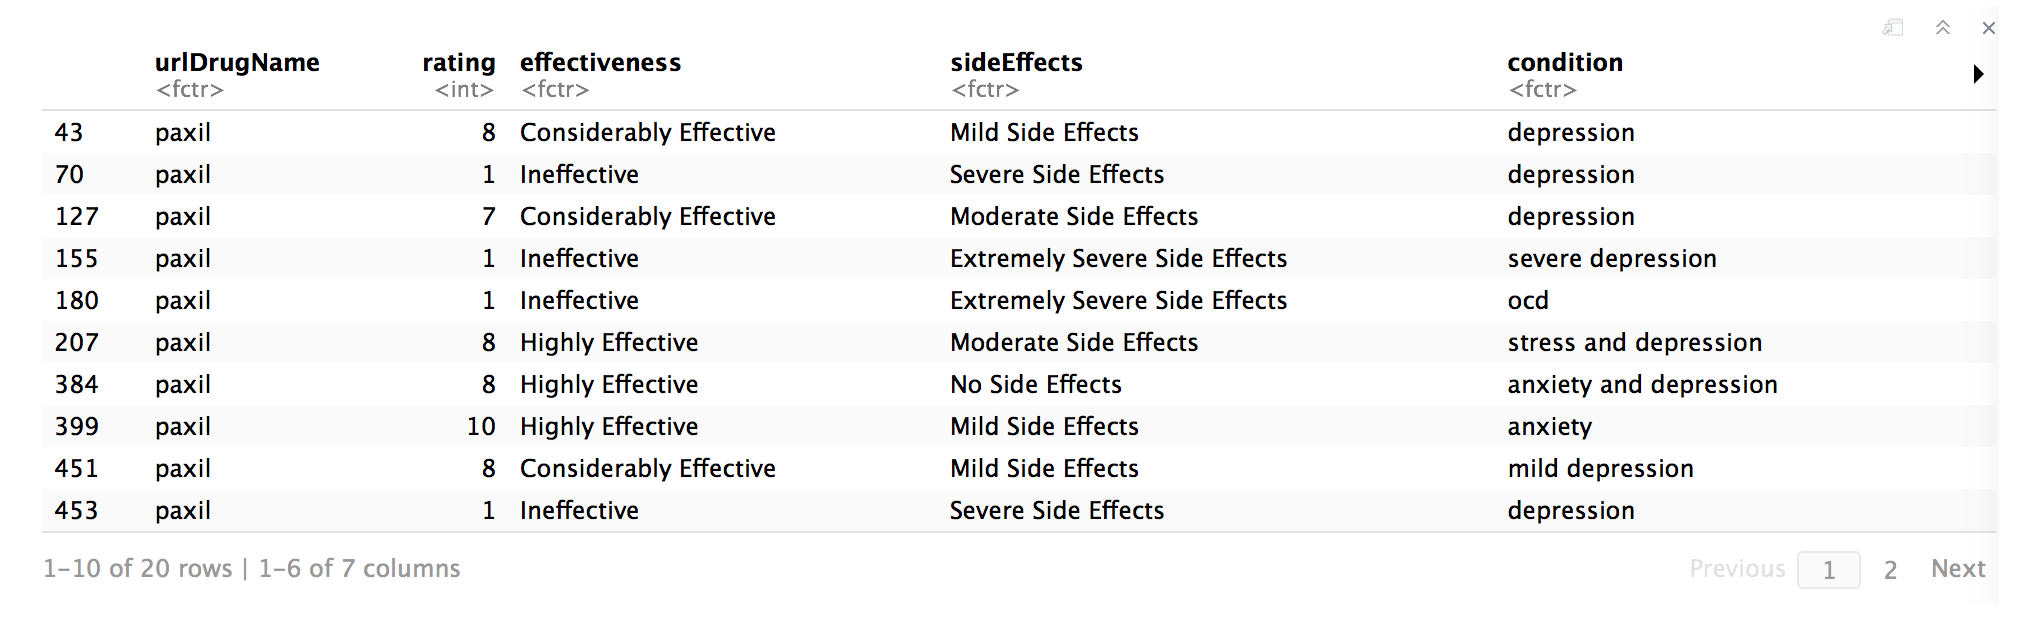
\includegraphics[width=0.85\textwidth]{imagenes/medicamentos_duplicados.png}
    \caption{Medicamento "paxil" repetido 20 veces en el conjunto test}
    \label{medicamentos_repetidos}
\end{figure}

\subsubsection{2.2.4. Cuantificación de
variables}\label{cuantificacion-de-variables}

Para poder analizar y trabajar más fácilmente con la información de
\emph{sideEffects} y \emph{effectiveness}, se va a realizar una
conversión de dichas columnas a un valor con el que nos sea más sencillo
trabajar.En otras palabras, vamos a asignar una etiqueta numérica a cada
valor pertinente, tanto para para \emph{train} como \emph{test}.

A continuación, vamos a cuantificar la columna de \emph{sideEffects},
para ello se añade una nueva columna a nuestro conjunto de datos
denominada \emph{sideEffectsNumber} que nos clasifica los posibles
valores de la columna \emph{sideEffects} en un rango numérico,
comprendido entre 1 y 5. Dicha columna hace referencia a la
clasificación de los efectos secundarios del medicamento según el
paciente, en donde la etiqueta con valor 1 hará referencia a que no haya
ningún efecto secundario y la etiqueta con valor 5 a que tiene efectos
secundarios extremadamente graves:

\begin{itemize}
\tightlist
\item
  Extremely Severe Side Effects (efectos secundarios extremadamente
  graves) : 5
\item
  Severe Side Effects (efectos secundarios graves): 4
\item
  Moderate Side Effects (efectos secundarios moderados) : 3
\item
  Mild Side Effects (efectos secundarios leves) : 2
\item
  No Side Effects (sin efectos secundarios) : 1
\end{itemize}

\begin{Shaded}
\begin{Highlighting}[]
\CommentTok{# Datos Train}
\NormalTok{datos_train}\OperatorTok{$}\NormalTok{sideEffectsNumber[datos_train}\OperatorTok{$}\NormalTok{sideEffects}\OperatorTok{==}\StringTok{"Extremely Severe Side Effects"}\NormalTok{]<-}\DecValTok{5}
\NormalTok{datos_train}\OperatorTok{$}\NormalTok{sideEffectsNumber[datos_train}\OperatorTok{$}\NormalTok{sideEffects}\OperatorTok{==}\StringTok{"Severe Side Effects"}\NormalTok{]<-}\DecValTok{4}
\NormalTok{datos_train}\OperatorTok{$}\NormalTok{sideEffectsNumber[datos_train}\OperatorTok{$}\NormalTok{sideEffects}\OperatorTok{==}\StringTok{"Moderate Side Effects"}\NormalTok{] <-}\StringTok{ }\DecValTok{3}
\NormalTok{datos_train}\OperatorTok{$}\NormalTok{sideEffectsNumber[datos_train}\OperatorTok{$}\NormalTok{sideEffects}\OperatorTok{==}\StringTok{"Mild Side Effects"}\NormalTok{]<-}\StringTok{ }\DecValTok{2}
\NormalTok{datos_train}\OperatorTok{$}\NormalTok{sideEffectsNumber[datos_train}\OperatorTok{$}\NormalTok{sideEffects}\OperatorTok{==}\StringTok{"No Side Effects"}\NormalTok{]<-}\StringTok{ }\DecValTok{1}

\CommentTok{# Datos Test}
\NormalTok{datos_test}\OperatorTok{$}\NormalTok{sideEffectsNumber[datos_test}\OperatorTok{$}\NormalTok{sideEffects}\OperatorTok{==}\StringTok{"Extremely Severe Side Effects"}\NormalTok{]<-}\DecValTok{5}
\NormalTok{datos_test}\OperatorTok{$}\NormalTok{sideEffectsNumber[datos_test}\OperatorTok{$}\NormalTok{sideEffects}\OperatorTok{==}\StringTok{"Severe Side Effects"}\NormalTok{]<-}\DecValTok{4}
\NormalTok{datos_test}\OperatorTok{$}\NormalTok{sideEffectsNumber[datos_test}\OperatorTok{$}\NormalTok{sideEffects}\OperatorTok{==}\StringTok{"Moderate Side Effects"}\NormalTok{]<-}\DecValTok{3}
\NormalTok{datos_test}\OperatorTok{$}\NormalTok{sideEffectsNumber[datos_test}\OperatorTok{$}\NormalTok{sideEffects}\OperatorTok{==}\StringTok{"Mild Side Effects"}\NormalTok{]<-}\DecValTok{2}
\NormalTok{datos_test}\OperatorTok{$}\NormalTok{sideEffectsNumber[datos_test}\OperatorTok{$}\NormalTok{sideEffects}\OperatorTok{==}\StringTok{"No Side Effects"}\NormalTok{]<-}\DecValTok{1}
\end{Highlighting}
\end{Shaded}

Podemos comprobar que se ha creado la nueva columna
\emph{sideEffectsNumber}, y que se han añadido los cambios comentados
anteriormente.

\begin{Shaded}
\begin{Highlighting}[]
\KeywordTok{head}\NormalTok{(datos_train}\OperatorTok{$}\NormalTok{sideEffects, }\DecValTok{5}\NormalTok{)}
\end{Highlighting}
\end{Shaded}

\begin{verbatim}
## [1] Mild Side Effects   Severe Side Effects No Side Effects    
## [4] Mild Side Effects   Severe Side Effects
## 5 Levels: Extremely Severe Side Effects ... Severe Side Effects
\end{verbatim}

\begin{Shaded}
\begin{Highlighting}[]
\KeywordTok{head}\NormalTok{(datos_train}\OperatorTok{$}\NormalTok{sideEffectsNumber, }\DecValTok{5}\NormalTok{) }
\end{Highlighting}
\end{Shaded}

\begin{verbatim}
## [1] 2 4 1 2 4
\end{verbatim}

Volvemos a aplicar el mismo procedimiento para la columna de
\emph{effectiveness}, creándonos para ello una columna denominada
\emph{effectivenessNumber}. Dicha columna, hace referencia a la
clasificación de la efectividad del medicamento según el paciente.
Asignaremos la etiqueta con valor 1 para indicar que el medicamente es
ineficaz, si este es altamente eficaz, le asignaremos la etiqueta con
valor 5:

\begin{itemize}
\tightlist
\item
  Highly Effective (altamente efectivo): 5
\item
  Considerably Effective (considerablemente efectivo) : 4
\item
  Moderately Effective (moderadamente efectivo) : 3
\item
  Marginally Effective (marginalmente efectivo) : 2
\item
  Ineffective (ineficaz) : 1
\end{itemize}

\begin{Shaded}
\begin{Highlighting}[]
\CommentTok{# Datos de entrenamiento}
\NormalTok{datos_train}\OperatorTok{$}\NormalTok{effectivenessNumber[datos_train}\OperatorTok{$}\NormalTok{effectiveness}\OperatorTok{==}\StringTok{"Highly Effective"}\NormalTok{]<-}\DecValTok{5}
\NormalTok{datos_train}\OperatorTok{$}\NormalTok{effectivenessNumber[datos_train}\OperatorTok{$}\NormalTok{effectiveness}\OperatorTok{==}\StringTok{"Considerably Effective"}\NormalTok{]<-}\DecValTok{4}
\NormalTok{datos_train}\OperatorTok{$}\NormalTok{effectivenessNumber[datos_train}\OperatorTok{$}\NormalTok{effectiveness}\OperatorTok{==}\StringTok{"Moderately Effective"}\NormalTok{]<-}\DecValTok{3}
\NormalTok{datos_train}\OperatorTok{$}\NormalTok{effectivenessNumber[datos_train}\OperatorTok{$}\NormalTok{effectiveness}\OperatorTok{==}\StringTok{"Marginally Effective"}\NormalTok{]<-}\DecValTok{2}
\NormalTok{datos_train}\OperatorTok{$}\NormalTok{effectivenessNumber[datos_train}\OperatorTok{$}\NormalTok{effectiveness}\OperatorTok{==}\StringTok{"Ineffective"}\NormalTok{]<-}\StringTok{ }\DecValTok{1}

\CommentTok{# Datos de test}
\NormalTok{datos_test}\OperatorTok{$}\NormalTok{effectivenessNumber[datos_test}\OperatorTok{$}\NormalTok{effectiveness}\OperatorTok{==}\StringTok{"Highly Effective"}\NormalTok{]<-}\DecValTok{5}
\NormalTok{datos_test}\OperatorTok{$}\NormalTok{effectivenessNumber[datos_test}\OperatorTok{$}\NormalTok{effectiveness}\OperatorTok{==}\StringTok{"Considerably Effective"}\NormalTok{]<-}\DecValTok{4}
\NormalTok{datos_test}\OperatorTok{$}\NormalTok{effectivenessNumber[datos_test}\OperatorTok{$}\NormalTok{effectiveness}\OperatorTok{==}\StringTok{"Moderately Effective"}\NormalTok{]<-}\DecValTok{3}
\NormalTok{datos_test}\OperatorTok{$}\NormalTok{effectivenessNumber[datos_test}\OperatorTok{$}\NormalTok{effectiveness}\OperatorTok{==}\StringTok{"Marginally Effective"}\NormalTok{]<-}\DecValTok{2}
\NormalTok{datos_test}\OperatorTok{$}\NormalTok{effectivenessNumber[datos_test}\OperatorTok{$}\NormalTok{effectiveness}\OperatorTok{==}\StringTok{"Ineffective"}\NormalTok{]<-}\DecValTok{1}
\end{Highlighting}
\end{Shaded}

Comprobamos que se ha creado la nueva columna
\emph{effectivenessNumber}, y que se han añadido los nuevos cambios.

\begin{Shaded}
\begin{Highlighting}[]
\KeywordTok{head}\NormalTok{(datos_train}\OperatorTok{$}\NormalTok{effectiveness, }\DecValTok{5}\NormalTok{)}
\end{Highlighting}
\end{Shaded}

\begin{verbatim}
## [1] Highly Effective     Highly Effective     Highly Effective    
## [4] Marginally Effective Marginally Effective
## 5 Levels: Considerably Effective Highly Effective ... Moderately Effective
\end{verbatim}

\begin{Shaded}
\begin{Highlighting}[]
\KeywordTok{head}\NormalTok{(datos_train}\OperatorTok{$}\NormalTok{effectivenessNumber, }\DecValTok{5}\NormalTok{) }
\end{Highlighting}
\end{Shaded}

\begin{verbatim}
## [1] 5 5 5 2 2
\end{verbatim}

\subsubsection{2.2.5. Cálculo del rating
ponderado}\label{calculo-del-rating-ponderado}

En este subapartado, se va a realizar una agregación de varias columnas,
en donde queremos realizar una valoración general del medicamento. Para
ello, se va a realizar una ponderación entre la columna que contiene los
efectos secundarios y la efectividad del medicamento. Asimismo, se ha
considerado los efectos secundarios del medicamento con mayor
importancia, es por eso que se le ha otorgado una ponderación del 70\%
frente al 30\% de la efectividad del medicamento.

\[( sideEffects \cdot 0.7 ) + ( effectiveness \cdot 0.3 )\]

El motivo de esta ponderación es que se considera que es peor tener
efectos secundarios severos en un medicamento, que ser efectivo. Dicha
agregación se ha añadido a una nueva columna, denominada
\textbf{weightedRating}, cuyo resultado contiene una valoración general
del medicamento. En donde, dicha transformación, puede ser usada para
realizar una comparación con las propias valoraciones de los usuarios.
Este cambio, nos permitirá trabajar posteriormente de una manera más
sencilla y simplificada.

\begin{Shaded}
\begin{Highlighting}[]
\CommentTok{# Recorremos el dataframe para el conjunto train}
\ControlFlowTok{for}\NormalTok{ (i }\ControlFlowTok{in} \DecValTok{1}\OperatorTok{:}\KeywordTok{length}\NormalTok{(datos_train[[}\DecValTok{1}\NormalTok{]])) \{}
  
  \CommentTok{# Obtenemos el valor de sideEffect}
\NormalTok{  sideEffectNumber <-}\StringTok{ }\NormalTok{datos_train}\OperatorTok{$}\NormalTok{sideEffectsNumber[i]}
  \CommentTok{# Obtenemos el valor de efectiveness}
\NormalTok{  effectivenessRating <-}\StringTok{ }\NormalTok{datos_train}\OperatorTok{$}\NormalTok{effectivenessNumber[i]}
  
  \CommentTok{# Inicializamos la variable}
\NormalTok{  sideEffectRating <-}\StringTok{ }\DecValTok{0}
  
  \CommentTok{# Convertimos el valor de sideEffect a la misma escala que efectiveness, ya que }
  \CommentTok{# sideEffect == 1 significa que no tiene efectos secundarios (lo cual es bueno), }
  \CommentTok{# y efecctiveness == 1 significa que no es efectivo (lo cual no es bueno). Para }
  \CommentTok{# ello realizamos la siguiente conversión:}
  \ControlFlowTok{if}\NormalTok{(sideEffectNumber }\OperatorTok{==}\StringTok{ }\DecValTok{1}\NormalTok{)}
\NormalTok{     sideEffectRating <-}\StringTok{ }\DecValTok{5}
  \ControlFlowTok{else} \ControlFlowTok{if}\NormalTok{(sideEffectNumber }\OperatorTok{==}\StringTok{ }\DecValTok{2}\NormalTok{)}
\NormalTok{    sideEffectRating <-}\StringTok{ }\DecValTok{4}
  \ControlFlowTok{else} \ControlFlowTok{if}\NormalTok{(sideEffectNumber }\OperatorTok{==}\StringTok{ }\DecValTok{3}\NormalTok{)}
\NormalTok{    sideEffectRating <-}\StringTok{ }\DecValTok{3}
  \ControlFlowTok{else} \ControlFlowTok{if}\NormalTok{(sideEffectNumber }\OperatorTok{==}\StringTok{ }\DecValTok{4}\NormalTok{)}
\NormalTok{    sideEffectRating <-}\StringTok{ }\DecValTok{2}
  \ControlFlowTok{else} \ControlFlowTok{if}\NormalTok{(sideEffectNumber }\OperatorTok{==}\StringTok{ }\DecValTok{5}\NormalTok{)}
\NormalTok{    sideEffectRating <-}\StringTok{ }\DecValTok{1}
  
  \CommentTok{# Obtenemos el resultado ponderado en tipo float}
\NormalTok{  floatResult <-}\StringTok{ }\NormalTok{effectivenessRating }\OperatorTok{*}\StringTok{ }\FloatTok{0.7} \OperatorTok{+}\StringTok{ }\NormalTok{sideEffectRating }\OperatorTok{*}\StringTok{ }\FloatTok{0.3}
  
  \CommentTok{# Convertimos el resultado a valor entero.}
\NormalTok{  integerResult <-}\StringTok{ }\KeywordTok{as.integer}\NormalTok{(floatResult)}
  
  \CommentTok{# Calculamos la parte decimal y redondeamos}
  \ControlFlowTok{if}\NormalTok{(floatResult }\OperatorTok{-}\StringTok{ }\NormalTok{integerResult }\OperatorTok{<}\StringTok{ }\FloatTok{0.5}\NormalTok{) result <-}\StringTok{ }\NormalTok{integerResult}
  \ControlFlowTok{else}\NormalTok{ result <-}\StringTok{ }\NormalTok{integerResult}\OperatorTok{+}\DecValTok{1}
  
  \CommentTok{# Añadimos el resultado obtenido y lo multiplicamos por dos para pasarlo a }
  \CommentTok{# escala (1-10)}
\NormalTok{  datos_train}\OperatorTok{$}\NormalTok{weightedRating[i] <-}\StringTok{ }\NormalTok{result }\OperatorTok{*}\StringTok{ }\DecValTok{2}
\NormalTok{\}}
\end{Highlighting}
\end{Shaded}

Comprobamos que se ha creado la nueva columna \emph{weightedRating}, y
que se han añadido los nuevos cambios.

\begin{Shaded}
\begin{Highlighting}[]
\KeywordTok{head}\NormalTok{(datos_train}\OperatorTok{$}\NormalTok{weightedRating, }\DecValTok{10}\NormalTok{) }
\end{Highlighting}
\end{Shaded}

\begin{verbatim}
##  [1] 10  8 10  6  4  2 10  8 10  2
\end{verbatim}

Ahora realizamos el mismo procesamiento para el conjunto test. Una vez
realizada la modificación, comprobamos que se ha creado la nueva columna
\emph{weightedRating}, y además que se han añadido los cambios
comentados.

\begin{Shaded}
\begin{Highlighting}[]
\KeywordTok{head}\NormalTok{(datos_test}\OperatorTok{$}\NormalTok{weightedRating, }\DecValTok{10}\NormalTok{) }
\end{Highlighting}
\end{Shaded}

\begin{verbatim}
##  [1]  8  8  4 10  8  8  6  8 10  2
\end{verbatim}

\subsubsection{2.2.6. Convertir el rating a variable
binaria}\label{convertir-el-rating-a-variable-binaria}

Para la realización de algunas técnicas que se explicarán más adelante,
se necesita tener una etiqueta o variable binaria comprendida entre 0 y
1. Es por eso que se ha optado por escoger la columna que contiene la
puntuación del medicamento por parte del paciente, y establecerla entre
0 y 1. En donde el 0, tendrá los valores comprendidos entre 1 y 4 y nos
indicará que el medicamento no es favorable; y en donde el 1, tendrá los
valores comprendidos entre 5 y 10 indicándonos que el medicamento es
favorable.

Dichos cambios, serán añadidos a una nueva columna llamada
\textbf{ratingLabel}. Realizamos dicho cambio, tanto para test como
train.

\begin{Shaded}
\begin{Highlighting}[]
\CommentTok{# Recorremos el dataframe para el conjunto train}
\ControlFlowTok{for}\NormalTok{ (i }\ControlFlowTok{in} \DecValTok{1}\OperatorTok{:}\KeywordTok{length}\NormalTok{(datos_train[[}\DecValTok{1}\NormalTok{]]))\{}
  
  \CommentTok{# Obtenemos el valor de rating}
\NormalTok{  rating <-}\StringTok{ }\NormalTok{datos_train}\OperatorTok{$}\NormalTok{rating[i]}
 
  \CommentTok{# Valores comprendidos entre 1 y 4 - no favorable - 0}
  \ControlFlowTok{if}\NormalTok{ (datos_train}\OperatorTok{$}\NormalTok{rating[i] }\OperatorTok{<}\StringTok{ }\DecValTok{5}\NormalTok{) result <-}\StringTok{ }\DecValTok{0}
  \CommentTok{# Valores comprendidos entre 5 y 10 - favorable - 1}
  \ControlFlowTok{else} \ControlFlowTok{if}\NormalTok{ (datos_train}\OperatorTok{$}\NormalTok{rating[i] }\OperatorTok{>=}\StringTok{ }\DecValTok{5}\NormalTok{) }
\NormalTok{    result <-}\StringTok{ }\DecValTok{1}
  
  \CommentTok{# Asignamos el resultado a la nueva variable}
\NormalTok{  datos_train}\OperatorTok{$}\NormalTok{ratingLabel[i] <-}\StringTok{ }\NormalTok{result}
\NormalTok{\}}
\end{Highlighting}
\end{Shaded}

\subsubsection{2.2.7. Cambiar el orden para la columna
sideEffectsNumber}\label{cambiar-el-orden-para-la-columna-sideeffectsnumber}

Al comparar las columna \emph{sideEffectsNumber} y
\emph{effectivenesNumber}, llegamos a la conclusión, de que ambas siguen
órdenes distintos, es decir, el valor 5 en \emph{sideEffectsNumber} dice
que el medicamento tiene efectos secundarios extremadamente graves, y el
valor 5 en \emph{effectivenesNumber} dice que el medicamento es
altamente efectivo. Por tanto, se ha considerado, que el valor
correspondiente al 5, sea positivo y el valor correspondiente a 1
negativo. Para ello, se ha modificado el orden de la columna
\emph{sideEffectsNumber}, en donde, la nueva columna
\textbf{sideEffectsInverse} tiene:

\begin{itemize}
\tightlist
\item
  Extremely Severe Side Effects (efectos secundarios extremadamente
  graves) : 1
\item
  Severe Side Effects (efectos secundarios graves): 2
\item
  Moderate Side Effects (efectos secundarios moderados) : 3
\item
  Mild Side Effects (efectos secundarios leves) : 4
\item
  No Side Effects (sin efectos secundarios) : 5
\end{itemize}

Realizamos dicha modificación, tanto para train como test. Con ello
buscamos, obtener resultados con los que nos resulte más cómodo de
trabajar.

\begin{Shaded}
\begin{Highlighting}[]
\CommentTok{# Recorremos el dataframe para el conjunto train}
\ControlFlowTok{for}\NormalTok{ (i }\ControlFlowTok{in} \DecValTok{1}\OperatorTok{:}\KeywordTok{length}\NormalTok{(datos_train[[}\DecValTok{1}\NormalTok{]]))\{}
  
  \CommentTok{# Obtenemos el valor de sideEffect}
\NormalTok{  sideEffectNumber <-}\StringTok{ }\NormalTok{datos_train}\OperatorTok{$}\NormalTok{sideEffectsNumber[i]}
  
  \CommentTok{# Inicializamos la variable}
\NormalTok{  sideEffectRating <-}\StringTok{ }\DecValTok{0}
  
  \CommentTok{# Cambiamos el orden para el el valor de sideEffect}
  \ControlFlowTok{if}\NormalTok{(sideEffectNumber }\OperatorTok{==}\StringTok{ }\DecValTok{1}\NormalTok{)}
\NormalTok{     sideEffectRating <-}\StringTok{ }\DecValTok{5}
  \ControlFlowTok{else} \ControlFlowTok{if}\NormalTok{(sideEffectNumber }\OperatorTok{==}\StringTok{ }\DecValTok{2}\NormalTok{)}
\NormalTok{    sideEffectRating <-}\StringTok{ }\DecValTok{4}
  \ControlFlowTok{else} \ControlFlowTok{if}\NormalTok{(sideEffectNumber }\OperatorTok{==}\StringTok{ }\DecValTok{3}\NormalTok{)}
\NormalTok{    sideEffectRating <-}\StringTok{ }\DecValTok{3}
  \ControlFlowTok{else} \ControlFlowTok{if}\NormalTok{(sideEffectNumber }\OperatorTok{==}\StringTok{ }\DecValTok{4}\NormalTok{)}
\NormalTok{    sideEffectRating <-}\StringTok{ }\DecValTok{2}
  \ControlFlowTok{else} \ControlFlowTok{if}\NormalTok{(sideEffectNumber }\OperatorTok{==}\StringTok{ }\DecValTok{5}\NormalTok{)}
\NormalTok{    sideEffectRating <-}\StringTok{ }\DecValTok{1}
 
  \CommentTok{# Añadimos el resultado obtenido}
\NormalTok{  datos_train}\OperatorTok{$}\NormalTok{sideEffectsInverse[i] <-}\StringTok{ }\NormalTok{sideEffectRating}
\NormalTok{\}}
\end{Highlighting}
\end{Shaded}

\begin{Shaded}
\begin{Highlighting}[]
\KeywordTok{head}\NormalTok{(datos_train}\OperatorTok{$}\NormalTok{sideEffectsNumber, }\DecValTok{10}\NormalTok{)}
\end{Highlighting}
\end{Shaded}

\begin{verbatim}
##  [1] 2 4 1 2 4 4 2 1 1 5
\end{verbatim}

\begin{Shaded}
\begin{Highlighting}[]
\KeywordTok{head}\NormalTok{(datos_train}\OperatorTok{$}\NormalTok{sideEffectsInverse, }\DecValTok{10}\NormalTok{)}
\end{Highlighting}
\end{Shaded}

\begin{verbatim}
##  [1] 4 2 5 4 2 2 4 5 5 1
\end{verbatim}

\subsubsection{2.2.8. Representación gráfica de los
datos}\label{representacion-grafica-de-los-datos}

Antes de comenzar con el análisis exploratorio, vamos realizar distintos
diagramas de barras con el fin de comprender mejor los datos, previo al
procesamiento. Primero realizaremos un diagrama de barras de las
clasificaciones del medicamento por parte del paciente.

En la figura \ref{grafica_rating}, se observa cómo más del 50\% de los
medicamentos obtienen una nota superior 6 por parte del paciente. Esto
nos sugiere que el paciente, tiene una buena opinión sobre un alto
porcentaje de los medicamentos, lo que puede dar lugar a opiniones más
positivas.

Por otro lado, vamos a mostrar gráficamente los efectos secundarios del
medicamento según el paciente. En donde el 1 significa que el
medicamento tiene pocos efectos secundarios y el 5 que tiene muchos
efectos secundarios. Como se aprecia en la figura
\ref{grafica_sideEffectsNumber}, un alto porcentaje de los medicamentos
no tiene efectos secundarios, de acuerdo a las valoraciones de los
pacientes.

\begin{figure}[ht]
    \centering
    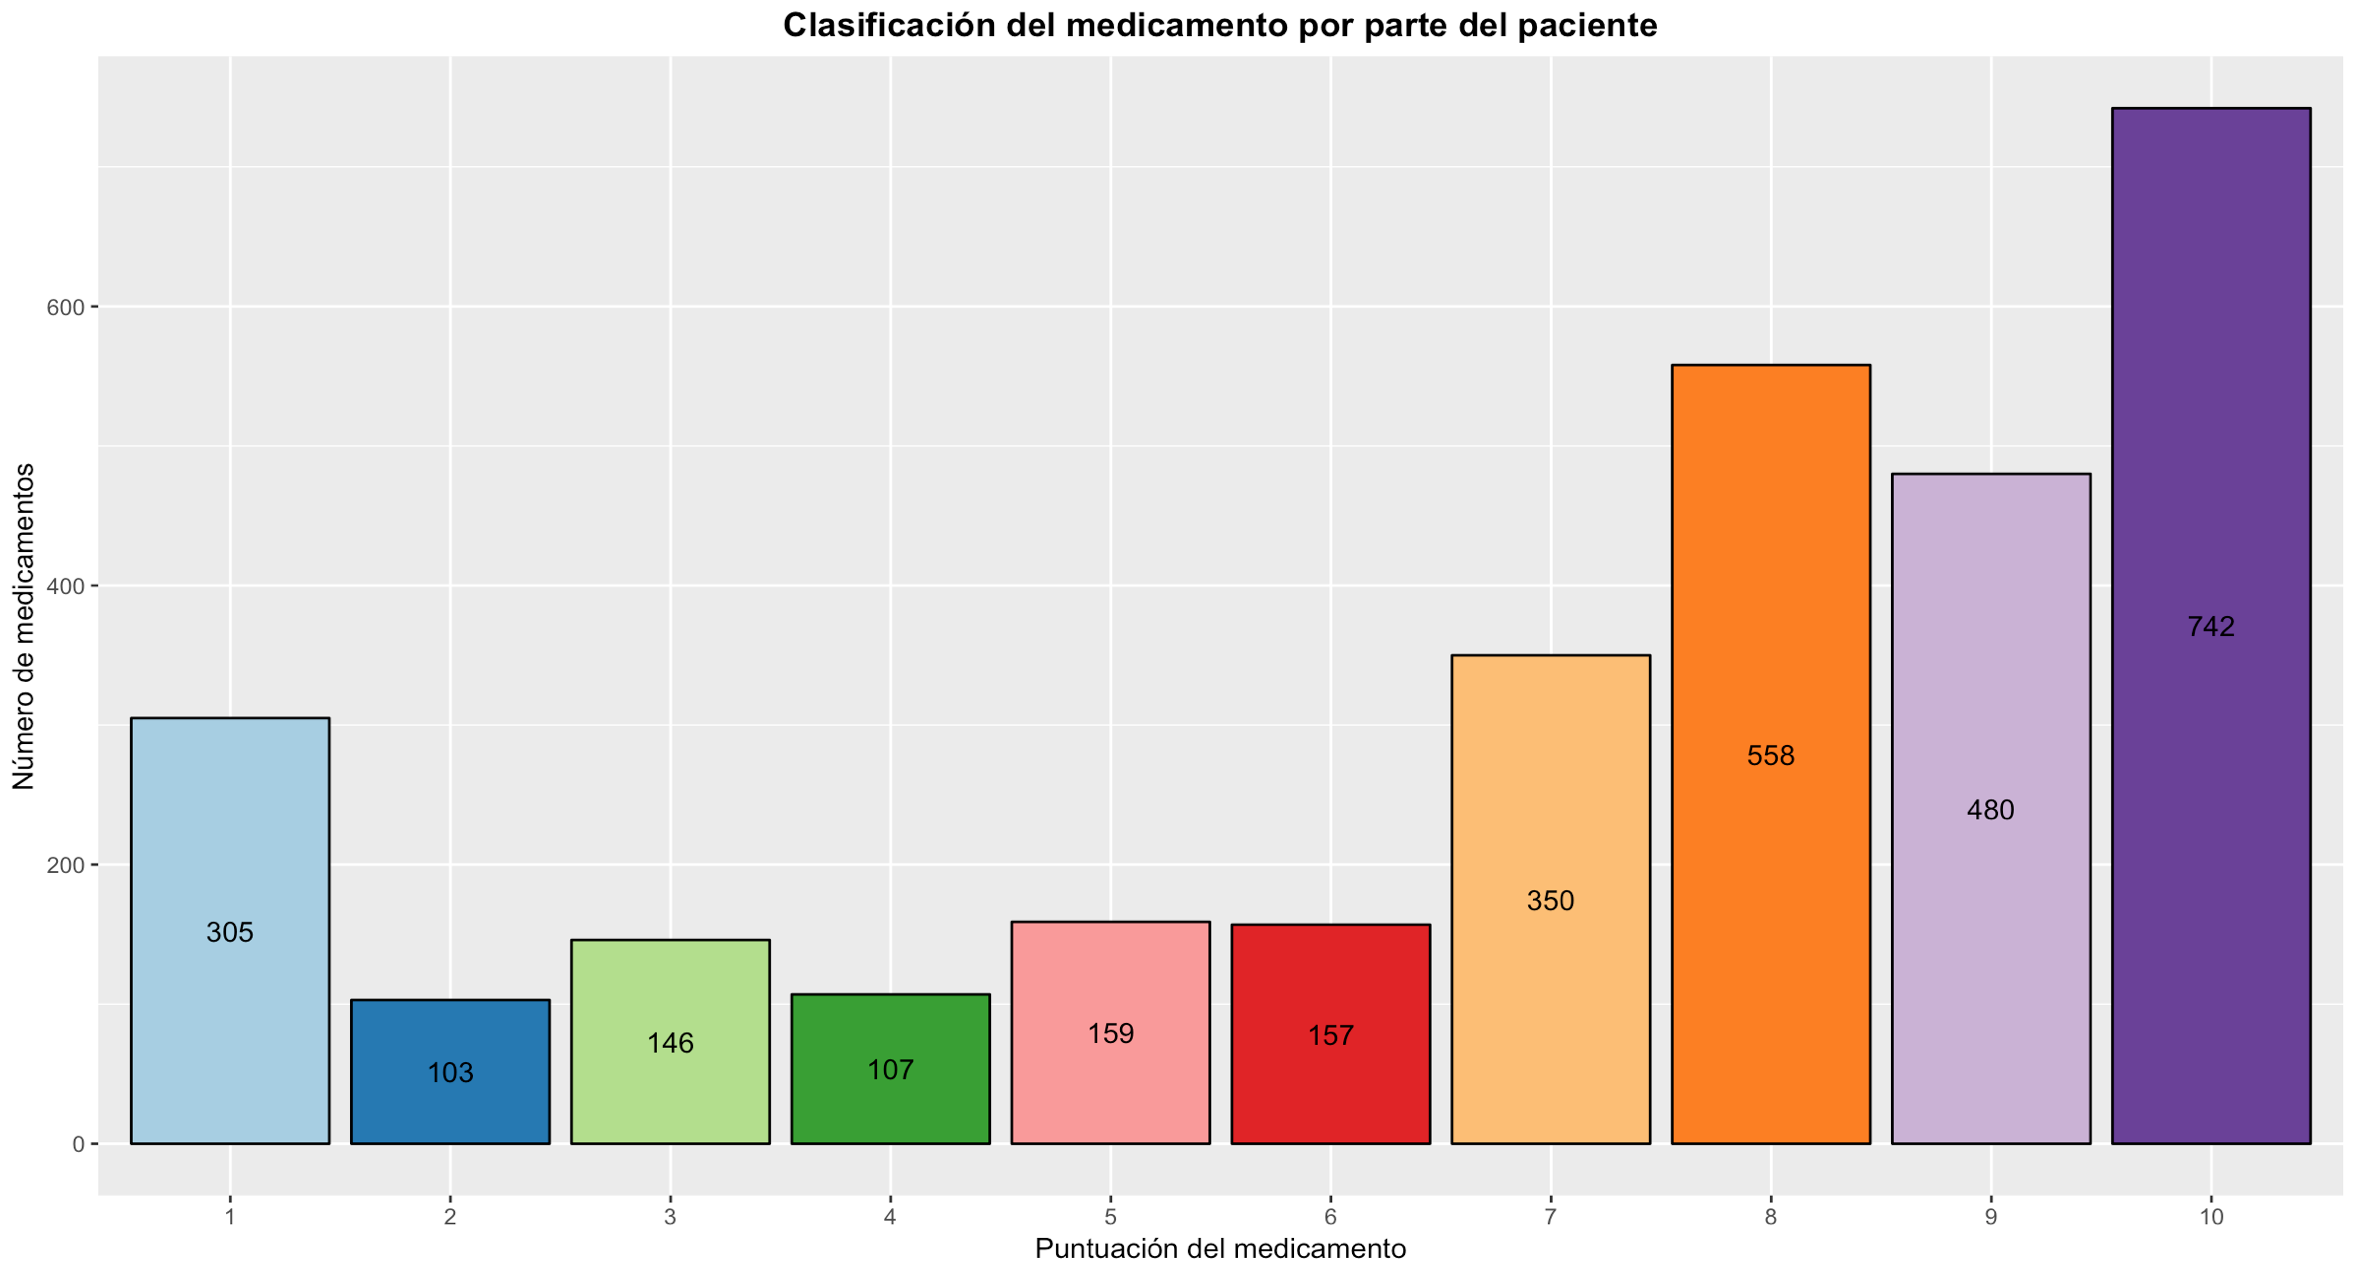
\includegraphics[width=0.76\textwidth]{imagenes/grafica_rating.png}
    \caption{Clasificación del medicamento por parte del paciente}
    \label{grafica_rating}
\end{figure}

\begin{figure}[ht]
    \centering
    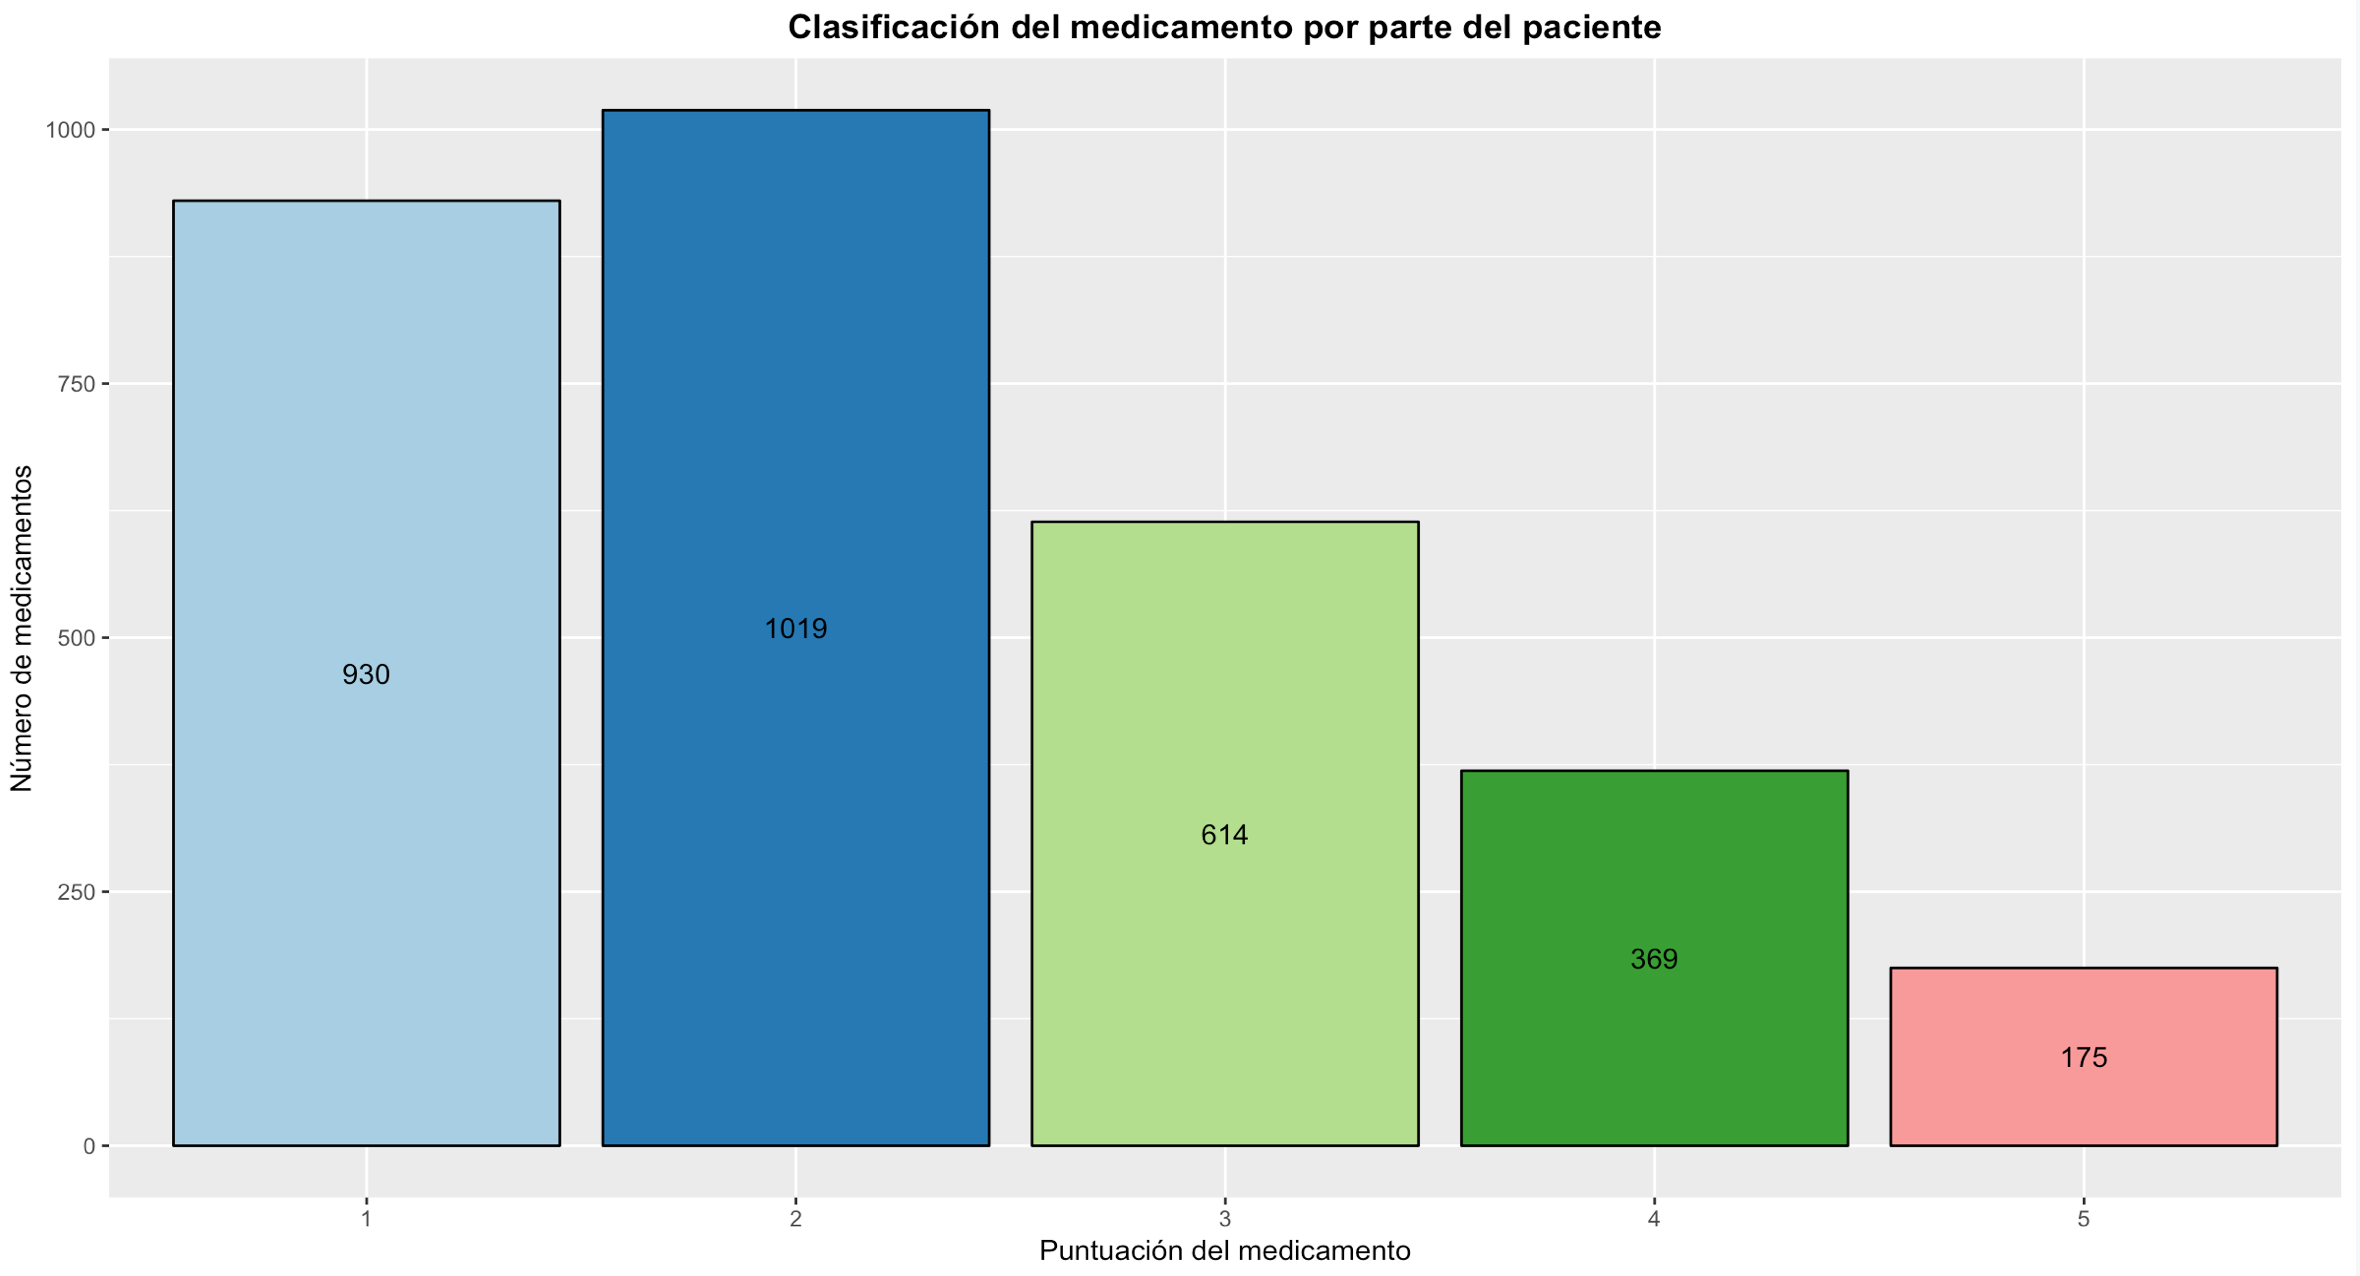
\includegraphics[width=0.76\textwidth]{imagenes/grafica_sideEffectsNumber.png}
    \caption{Clasificación de los efectos secundarios del medicamento según el paciente}
    \label{grafica_sideEffectsNumber}
\end{figure}

Por último, vamos a visualizar gráficamente, la efectividad del
medicamento según el paciente. En donde el 1 significa que el
medicamento tiene poca efectividad y el 5 que tiene mucha efectividad.
De acuerdo a la figura \ref{grafica_sideEffectsNumber}, es lógica esta
observación, sobretodo teniendo en cuenta el hecho de que, para los
medicamentos catalogados con pocos efectos secundarios, es de esperar
que los pacientes tengan buena opinión de ellos y se traduzca en una
alta efectividad.

\begin{figure}[h]
    \centering
    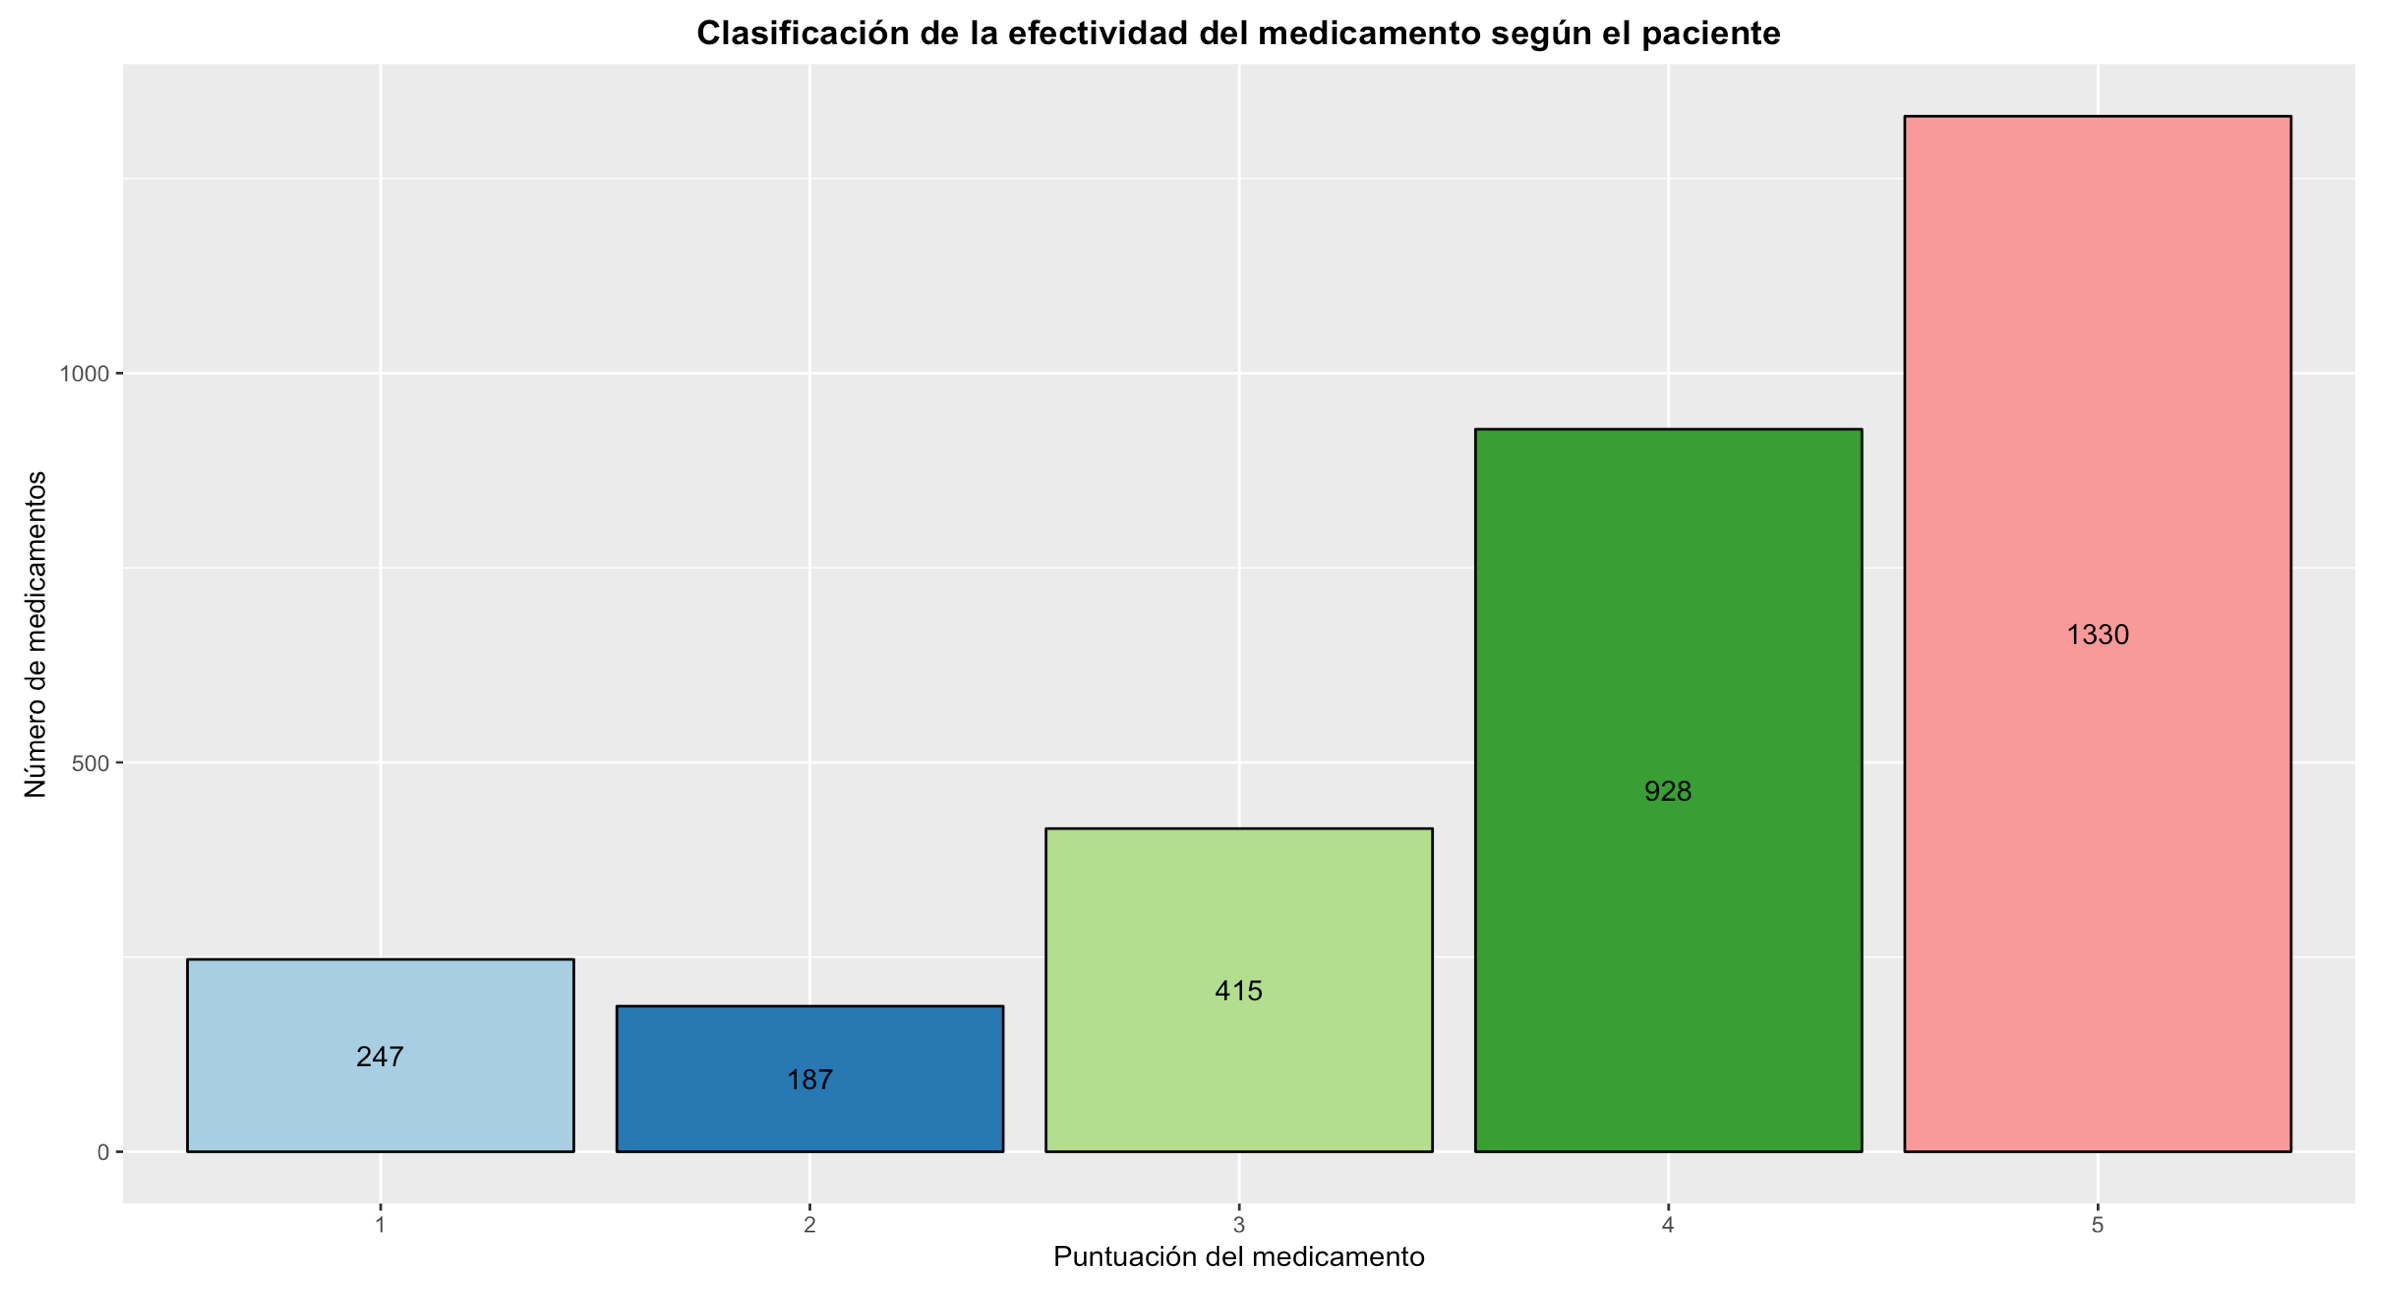
\includegraphics[width=0.76\textwidth]{imagenes/grafica_effectivenessNumber.png}
    \caption{Clasificación de la efectividad del medicamento según el paciente}
    \label{grafica_sideEffectsNumber}
\end{figure}

Acabamos de comprobar, cómo las valoraciones de los medicamentos por
parte de los pacientes son mayormente positivas. Por tanto, una vez
comprendidos los datos y eliminadas las columnas anteriores y
modificadas las necesarias, ya podemos continuar con el procesamiento de
los datos. Para ello, lo primero tenemos que hacer es cargar la librería
que procesa los datos de tipo texto en R, para la construcción y
manipulación del corpus. La librería más conocida se llama \textbf{tm},
aunque también haremos uso del paquete \textbf{SnowballC} para realizar
el \emph{Stemming}.

\subsubsection{2.2.9. Creación del corpus}\label{creacion-del-corpus}

Para poder obtener la estructura con la que vamos a procesar nuestra
información, debemos obtener un vector con documentos. En nuestro caso,
cada uno de los documentos se corresponde con una opinión sobre un
fármaco (\emph{benefitsReview}) y los efectos que tiene
(\emph{sideEffectsReview}). Para ello, primero debemos de construir un
vector con todas los opiniones del \emph{dataframe} y convertir cada
elemento del vector al formato de documento. Podemos usar la función
\emph{VectorSource} para hacer esta conversión. Se deberán realizar
todas las modificaciones tanto para el conjunto train como test.

\begin{Shaded}
\begin{Highlighting}[]
\CommentTok{# Datos train}

\CommentTok{# Nos quedamos con la única columna del dataset que nos interesa. }
\CommentTok{# Necesitamos obtenerla en forma de vector, y no como un dataframe de una columna, }
\CommentTok{# por lo que usamos as.vector para hacer la conversión}
\NormalTok{benefits_train_review_data =}\StringTok{ }\KeywordTok{as.vector}\NormalTok{(datos_train}\OperatorTok{$}\NormalTok{benefitsReview)}
\NormalTok{effects_train_review_data =}\StringTok{ }\KeywordTok{as.vector}\NormalTok{(datos_train}\OperatorTok{$}\NormalTok{sideEffectsReview)}

\CommentTok{# Lo convertimos en la estructura de documento, y lo guardamos ya en el corpus }
\CommentTok{# que lo vamos a utilizar}
\NormalTok{benefits_train_corpus =}\StringTok{ }\NormalTok{(}\KeywordTok{VectorSource}\NormalTok{(benefits_train_review_data))}
\NormalTok{effects_train_corpus =}\StringTok{ }\NormalTok{(}\KeywordTok{VectorSource}\NormalTok{(effects_train_review_data))}

\CommentTok{# Creamos el propio corpus}
\NormalTok{benefits_train_corpus <-}\StringTok{ }\KeywordTok{Corpus}\NormalTok{(benefits_train_corpus)}
\NormalTok{effects_train_corpus <-}\StringTok{ }\KeywordTok{Corpus}\NormalTok{(effects_train_corpus)}
\end{Highlighting}
\end{Shaded}

\begin{Shaded}
\begin{Highlighting}[]
\CommentTok{# Datos test}

\CommentTok{# Nos quedamos con la única columna del dataset que nos interesa. }
\CommentTok{# Necesitamos obtenerla en forma de vector, y no como un dataframe de una columna, }
\CommentTok{# por lo que usamos as.vector para hacer la conversión}
\NormalTok{benefits_test_review_data =}\StringTok{ }\KeywordTok{as.vector}\NormalTok{(datos_test}\OperatorTok{$}\NormalTok{benefitsReview)}
\NormalTok{effects_test_review_data =}\StringTok{ }\KeywordTok{as.vector}\NormalTok{(datos_test}\OperatorTok{$}\NormalTok{sideEffectsReview)}

\CommentTok{# Lo convertimos en la estructura de documento, y lo guardamos ya en el corpus }
\CommentTok{# que lo vamos a utilizar}
\NormalTok{benefits_test_corpus =}\StringTok{ }\NormalTok{(}\KeywordTok{VectorSource}\NormalTok{(benefits_test_review_data))}
\NormalTok{effects_test_corpus =}\StringTok{ }\NormalTok{(}\KeywordTok{VectorSource}\NormalTok{(effects_test_review_data))}

\CommentTok{# Creamos el propio corpus}
\NormalTok{benefits_test_corpus <-}\StringTok{ }\KeywordTok{Corpus}\NormalTok{(benefits_test_corpus)}
\NormalTok{effects_test_corpus <-}\StringTok{ }\KeywordTok{Corpus}\NormalTok{(effects_test_corpus)}
\end{Highlighting}
\end{Shaded}

Podemos ver que funciona accediendo a uno cualquiera, de la forma
\texttt{inspect(benefits\_train\_corpus{[}4{]})}:

\begin{figure}[h]
    \centering
    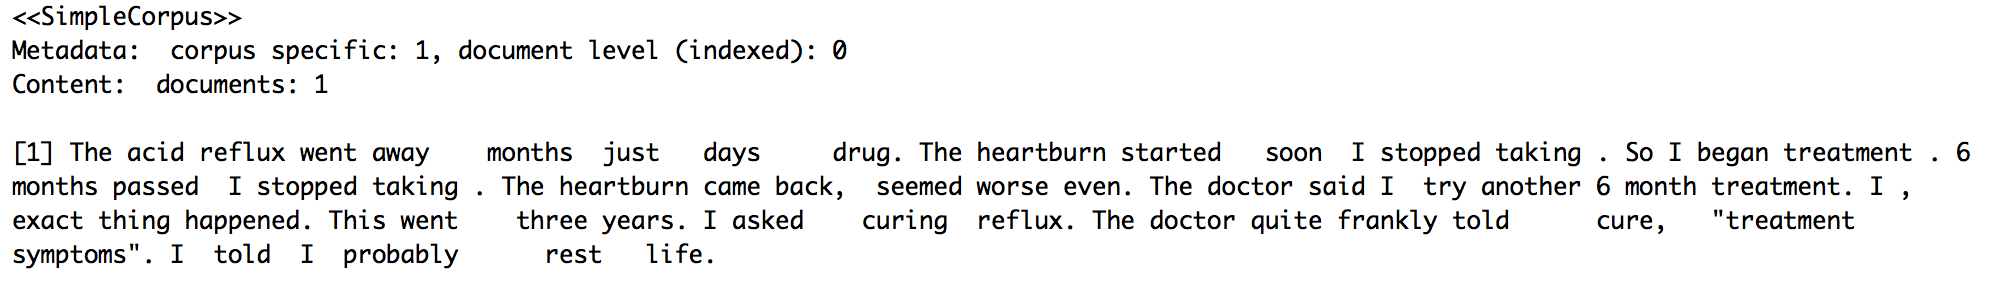
\includegraphics[width=1\textwidth]{imagenes/benefits_train_corpus1.png}
    \caption{Contenido para benefits\_train\_corpus I}
    \label{benefits1}
\end{figure}

O de la forma \texttt{benefits\_train\_corpus{[}{[}4{]}{]}\$content}:

\begin{figure}[h]
    \centering
    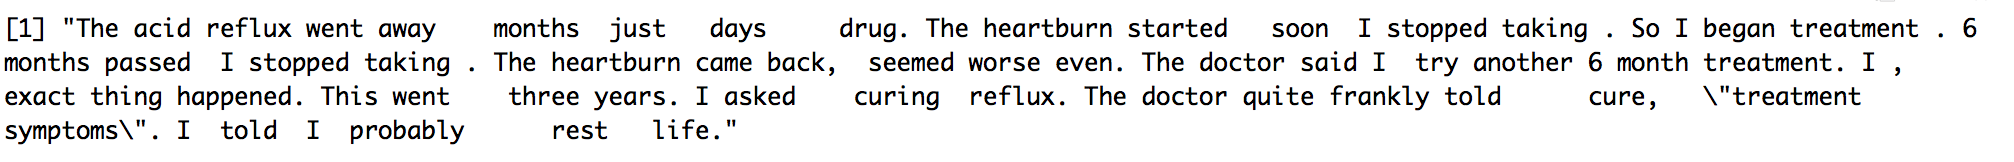
\includegraphics[width=1\textwidth]{imagenes/benefits_train_corpus2.png}
    \caption{Contenido para benefits\_train\_corpus II}
    \label{benefits2}
\end{figure}

Como aspecto a destactar, si nos fijamos en el contenido, podemos ver
que tiene signos de puntuación y exclamación.

\subsubsection{2.2.10. Correlación}\label{correlacion}

Una forma de medir la relación existente entre las variables en nuestro
dataset, es calcular la correlación entre un término y todos los demás
de la matriz. Como en este caso, estamos usando variables textuales, no
se aconseja hacer la correlación como tal. Debido a que la correlación
indica la fuerza y la dirección de una relación lineal y
proporcionalidad entre dos variables estadísticas, ya que está pensada
para variables cuantitativas. Por otro lado, sí que disponemos de
variables categóricas, pero también se ha despreciado hacer la
correlación entre ellas, debido a que no podemos prescindir de las
etiquetas, ni agrupar distintos medicamentos en uno solo.

Además, la correlación está relacionada con el análisis de componentes
principales (PCA), el cual, es una técnica utilizada para describir un
conjunto de datos en términos de nuevas variables no correlacionadas.
Por lo que se ha despreciado inicialmente realizar tal método.

\subsubsection{2.2.11. Representación gráfica de las frecuencias del
Corpus}\label{representacion-grafica-de-las-frecuencias-del-corpus}

Una vez creado el corpus y antes de aplicar las técnicas de
preprocesamiento, vamos a visualizar las frecuencias para las dos
columnas (\emph{benefitsReview} y \emph{sideEffectsReview}) de textos a
las que vamos aplicar el preprocesamiento. Para ello, debemos calcular
la matriz de términos y obtener los términos con mayor frecuencia.

Como se puede apreciar en la gráfica \ref{benefits3}, los términos que
más se repiten son \emph{the} y \emph{and}, además de otras
preposiciones y conjunciones. Si se observa, las palabras que aparecen
en la gráfica, no nos aportan información alguna, es por eso que vamos
hacer una transformación a los términos, como la eliminación de los
\emph{stopwords}.

A continuación, mostramos los términos para la columna
\emph{sideEffects}, realizando el mismo procedimiento que antes. Y como
se puede ver en la gráfica \ref{benefits4}, obtenemos la misma
conclusión, en donde tenemos palabras que no nos aportan nada de
información: \emph{very}, \emph{the}, \emph{that}, \emph{and}\ldots{}

\begin{figure}[ht]
    \centering
    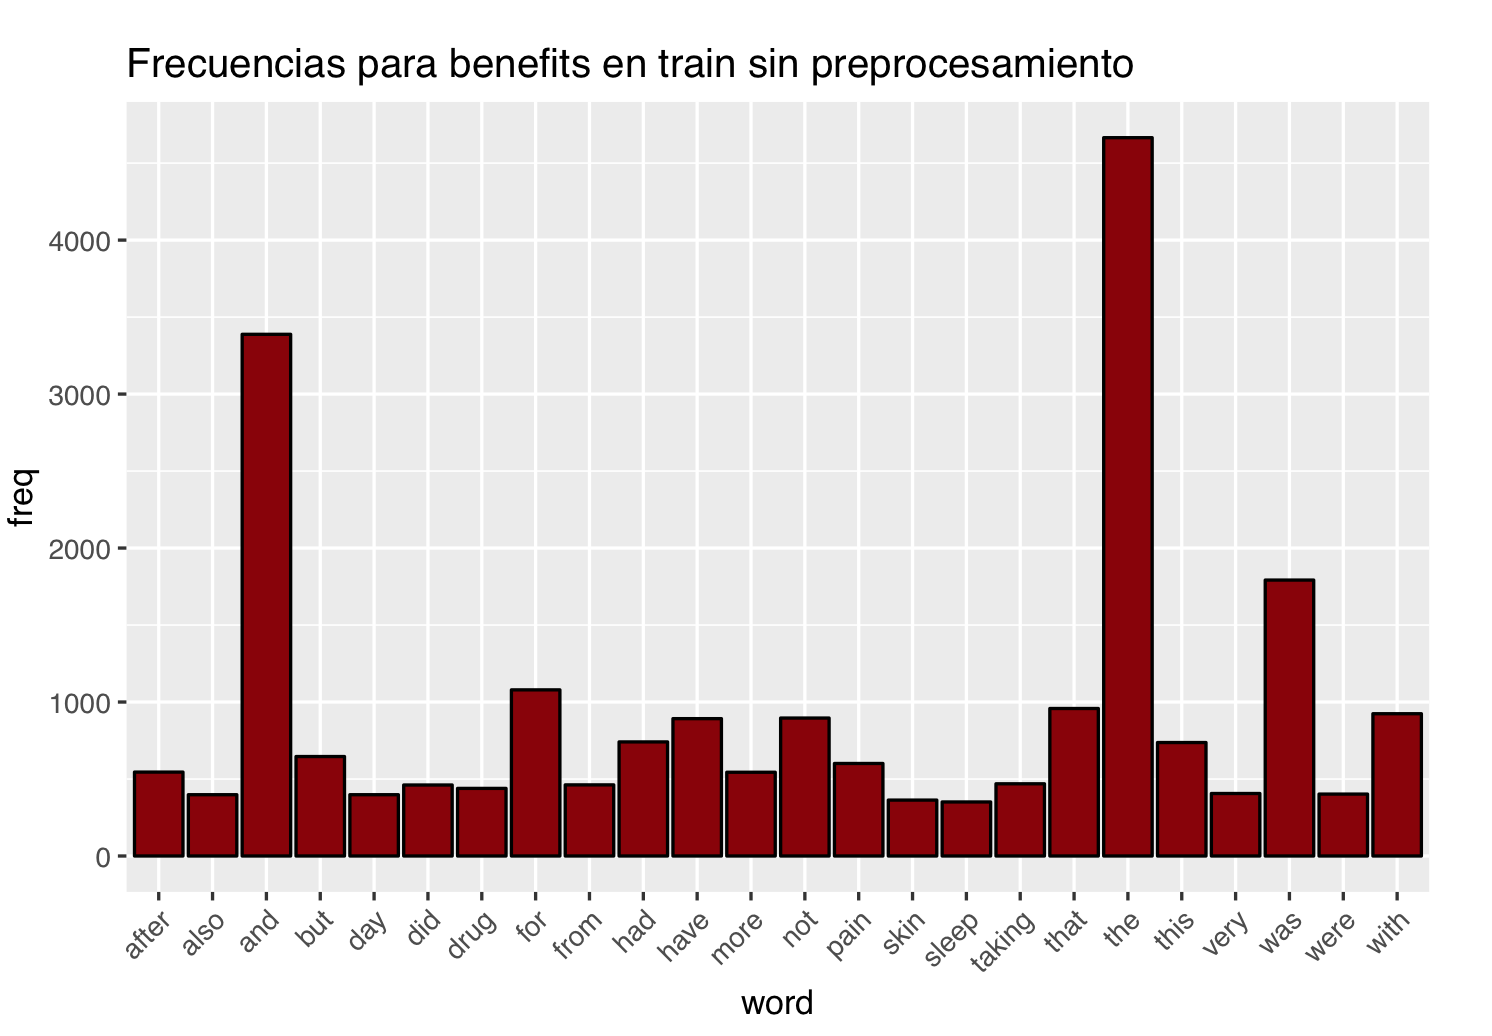
\includegraphics[width=0.67\textwidth]{imagenes/frecuencias_benefits.png}
    \caption{Frecuencia de términos para la columna benefitsReview}
    \label{benefits3}
\end{figure}

\begin{figure}[ht]
    \centering
    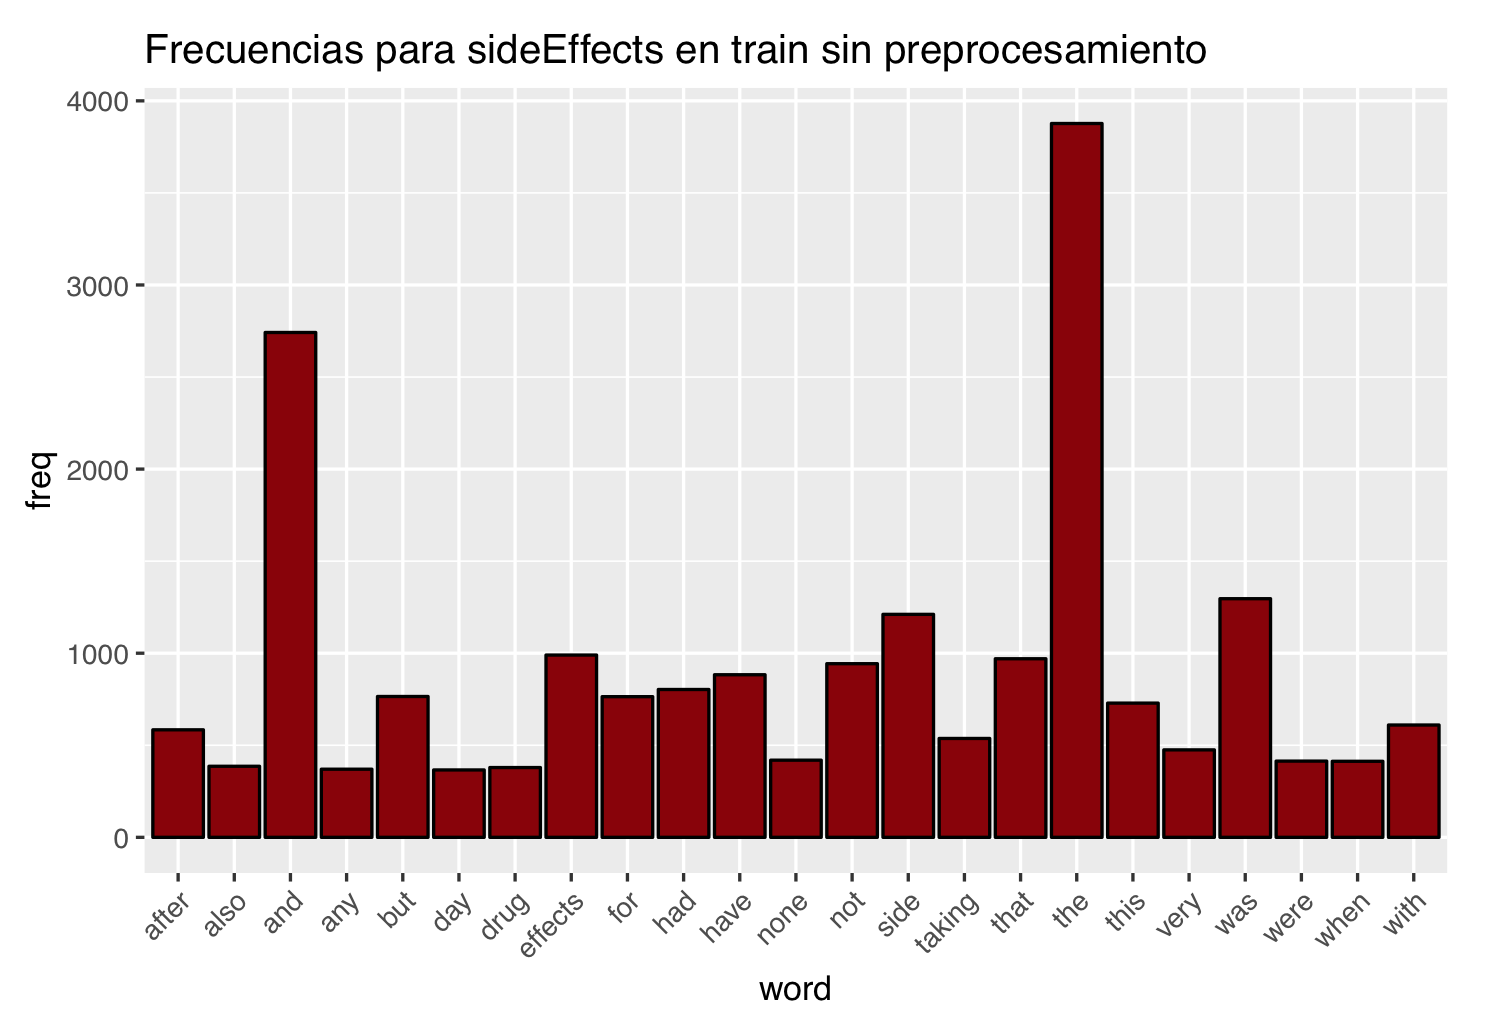
\includegraphics[width=0.67\textwidth]{imagenes/frecuencias_sideEffects.png}
    \caption{Frecuencia de términos para la columna sideEffectsReview}
    \label{benefits4}
\end{figure}

\subsubsection{2.2.12. Eliminar signos de
puntuación}\label{eliminar-signos-de-puntuacion}

Como hemos podido ver en el documento que se ha mostrado por pantalla,
en él se aprecia el uso de signos de puntuación y exclamación. En un
principio, no tiene sentido en \textit{Data Mining} contemplar los
signos de puntuación, ya que no nos van a aportar información. Por ello,
los quitamos, como se puede ver a continuación. Con
\texttt{tm\_map(corpus,\ removePunctuation)}, se eliminan los símbolos:
! " \$ \% \& `() * + , - . / : ; \textless{} = \textgreater{} ? @ {[}
~{]} \^{} \_' \{ \textbar{} \} \textasciitilde{}, tanto para train como
test.

\begin{Shaded}
\begin{Highlighting}[]
\CommentTok{# Una vez que tenemos el corpus creado, continuamos con el procesamiento para datos train}
\NormalTok{benefits_train_corpus <-}\StringTok{ }\KeywordTok{tm_map}\NormalTok{(benefits_train_corpus,}
                                \KeywordTok{content_transformer}\NormalTok{(removePunctuation))}
\NormalTok{effects_train_corpus <-}\StringTok{ }\KeywordTok{tm_map}\NormalTok{(effects_train_corpus, }
                               \KeywordTok{content_transformer}\NormalTok{(removePunctuation))}

\CommentTok{# Una vez que tenemos el corpus creado, continuamos con el procesamiento para datos test}
\NormalTok{benefits_test_corpus <-}\StringTok{ }\KeywordTok{tm_map}\NormalTok{(benefits_test_corpus, }
                               \KeywordTok{content_transformer}\NormalTok{(removePunctuation))}
\NormalTok{effects_test_corpus <-}\StringTok{ }\KeywordTok{tm_map}\NormalTok{(effects_test_corpus, }
                              \KeywordTok{content_transformer}\NormalTok{(removePunctuation))}
\end{Highlighting}
\end{Shaded}

Si volvemos a mostrar la opinión número cuatro, vemos como todos los
signos han desaparecido. De hecho, podemos inspeccionar el corpus, y se
ve como todos los signos de puntuación, exclamación y derivados ya no
están.

\begin{figure}[h]
    \centering
    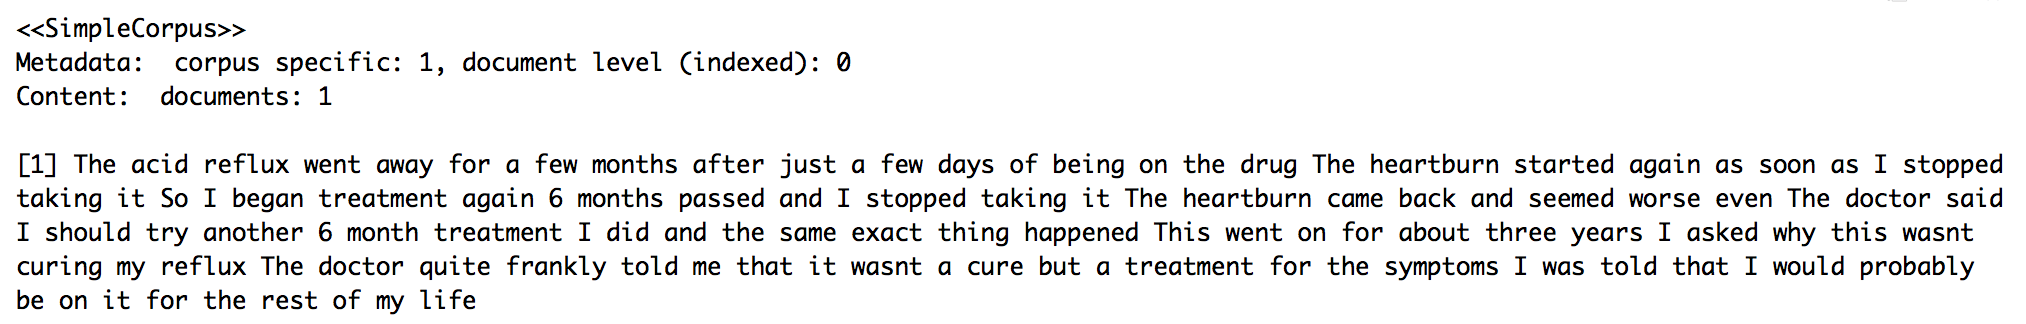
\includegraphics[width=1\textwidth]{imagenes/benefits_signos_puntuacion.png}
    \caption{Contenido de benefits sin signos de puntuación}
    \label{benefits2}
\end{figure}

Ocurre lo mismo con el comentario de efectos número siete.

\begin{figure}[h]
    \centering
    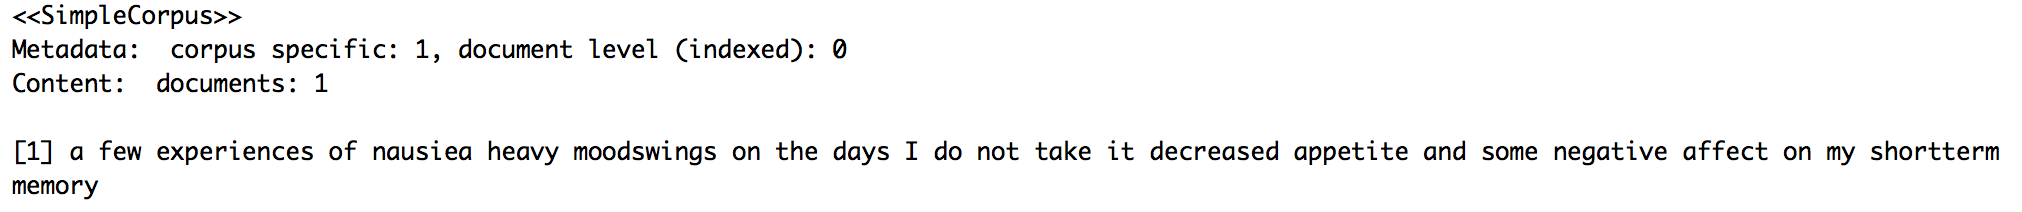
\includegraphics[width=1\textwidth]{imagenes/effects_signos_puntuacion.png}
    \caption{Contenido de effects sin signos de puntuación}
    \label{benefits2}
\end{figure}

\subsubsection{2.2.13. Conversión de las mayúsculas en
minúsculas}\label{conversion-de-las-mayusculas-en-minusculas}

Para poder hacer uso de los términos por igual, debemos convertir las
mayúsculas en minúsculas. Normalmente se convierte en minúsculas todas
las letras para que los comienzos de oración no sean tratados de manera
diferente por los algoritmos, tanto para train como test.

\begin{Shaded}
\begin{Highlighting}[]
\CommentTok{# Datos train}
\NormalTok{benefits_train_corpus <-}\StringTok{ }\KeywordTok{tm_map}\NormalTok{(benefits_train_corpus, }\KeywordTok{content_transformer}\NormalTok{(tolower))}
\NormalTok{effects_train_corpus <-}\StringTok{ }\KeywordTok{tm_map}\NormalTok{(effects_train_corpus, }\KeywordTok{content_transformer}\NormalTok{(tolower))}

\CommentTok{# Datos test}
\NormalTok{benefits_test_corpus <-}\StringTok{ }\KeywordTok{tm_map}\NormalTok{(benefits_test_corpus, }\KeywordTok{content_transformer}\NormalTok{(tolower))}
\NormalTok{effects_test_corpus <-}\StringTok{ }\KeywordTok{tm_map}\NormalTok{(effects_test_corpus, }\KeywordTok{content_transformer}\NormalTok{(tolower))}
\end{Highlighting}
\end{Shaded}

Si volvemos a mostrar las opiniones, vemos como todas las mayúsuculas
han desaparecido.

\begin{figure}[h]
    \centering
    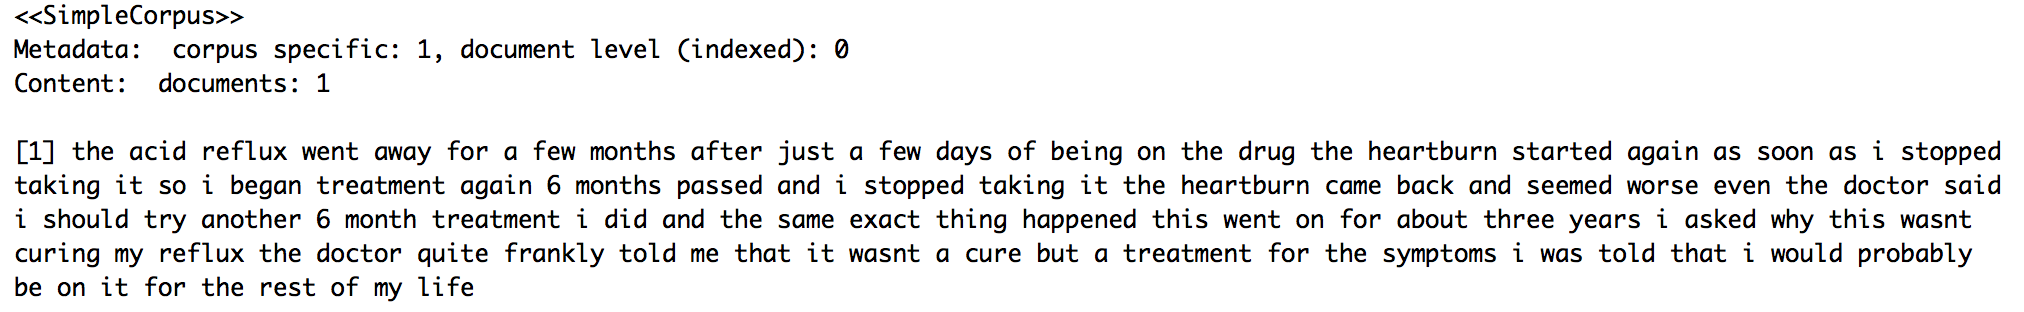
\includegraphics[width=1\textwidth]{imagenes/benefits_mayusculas.png}
    \caption{Contenido de benefits sin mayúsculas}
    \label{benefits2}
\end{figure}

\begin{figure}[h]
    \centering
    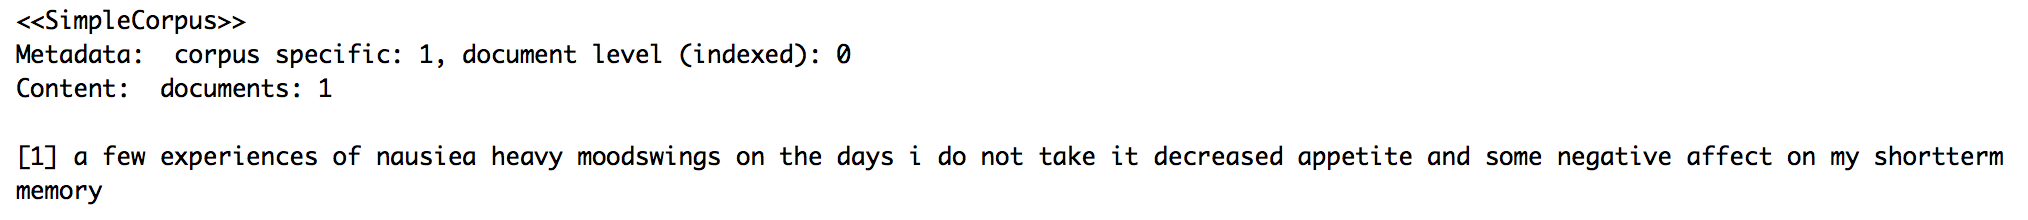
\includegraphics[width=1\textwidth]{imagenes/effects_mayusculas.png}
    \caption{Contenido de effects sin mayúsculas}
    \label{benefits2}
\end{figure}

\subsubsection{2.2.14. Eliminación de
Stopwords}\label{eliminacion-de-stopwords}

En cualquier idioma, hay palabras que son tan comunes o utilizadas que
no aportan información relevante, a dichas palabras se las conoce como
\emph{stopwords} o palabras \emph{stop}. Por ejemplo, en español, las
palabras ``la'', ``a'', ``en'', ``de'' son ejemplos de \emph{stopwords}.
Este tipo de palabras debemos de suprimirlas de nuestro corpus. Como, en
nuestro caso, el contenido del corpus está en inglés, debemos
especificar el idioma correcto para que nos elimine del corpus las
palabras adecuadas en dicho idioma, tanto en train como en test.

\begin{Shaded}
\begin{Highlighting}[]
\CommentTok{# Datos train}
\NormalTok{benefits_train_corpus <-}\StringTok{ }\KeywordTok{tm_map}\NormalTok{(benefits_train_corpus, }\KeywordTok{content_transformer}\NormalTok{(removeWords), }
                                \KeywordTok{stopwords}\NormalTok{(}\StringTok{"english"}\NormalTok{))}
\NormalTok{effects_train_corpus <-}\StringTok{ }\KeywordTok{tm_map}\NormalTok{(effects_train_corpus, }\KeywordTok{content_transformer}\NormalTok{(removeWords), }
                               \KeywordTok{stopwords}\NormalTok{(}\StringTok{"english"}\NormalTok{))}

\CommentTok{# Datos test}
\NormalTok{benefits_test_corpus <-}\StringTok{ }\KeywordTok{tm_map}\NormalTok{(benefits_test_corpus, }\KeywordTok{content_transformer}\NormalTok{(removeWords), }
                               \KeywordTok{stopwords}\NormalTok{(}\StringTok{"english"}\NormalTok{))}
\NormalTok{effects_test_corpus <-}\StringTok{ }\KeywordTok{tm_map}\NormalTok{(effects_test_corpus, }\KeywordTok{content_transformer}\NormalTok{(removeWords), }
                              \KeywordTok{stopwords}\NormalTok{(}\StringTok{"english"}\NormalTok{))}
\end{Highlighting}
\end{Shaded}

Si volvemos a mostrar las opiniones, vemos como por ejemplo las palabras
como \emph{the} o \emph{and}, han desaparecido de nuestro corpus.

\begin{figure}[h]
    \centering
    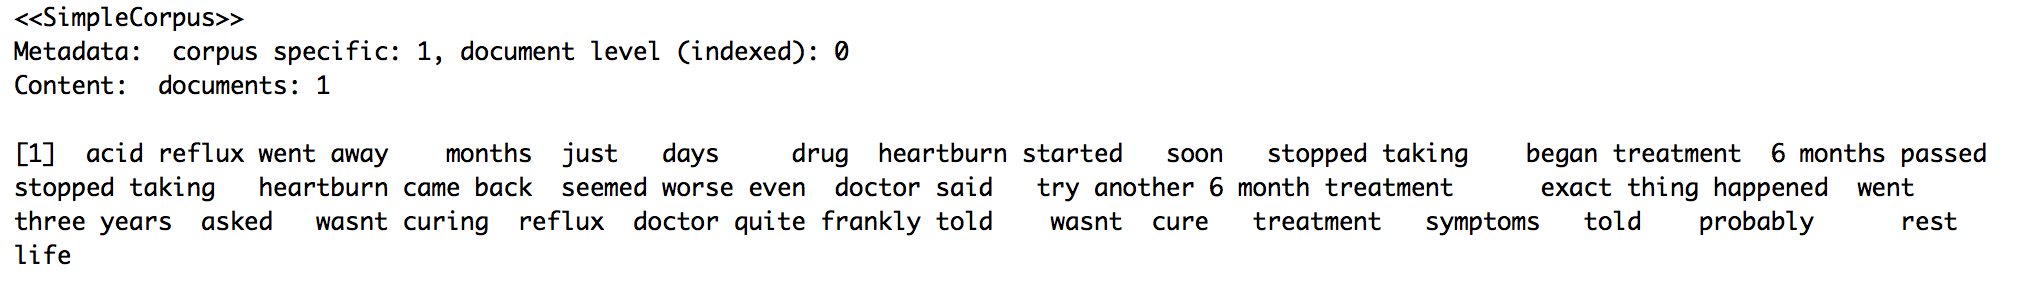
\includegraphics[width=1\textwidth]{imagenes/benefits_stopwords.png}
    \caption{Contenido de benefits sin stopwords}
    \label{benefits2}
\end{figure}

\begin{figure}[h]
    \centering
    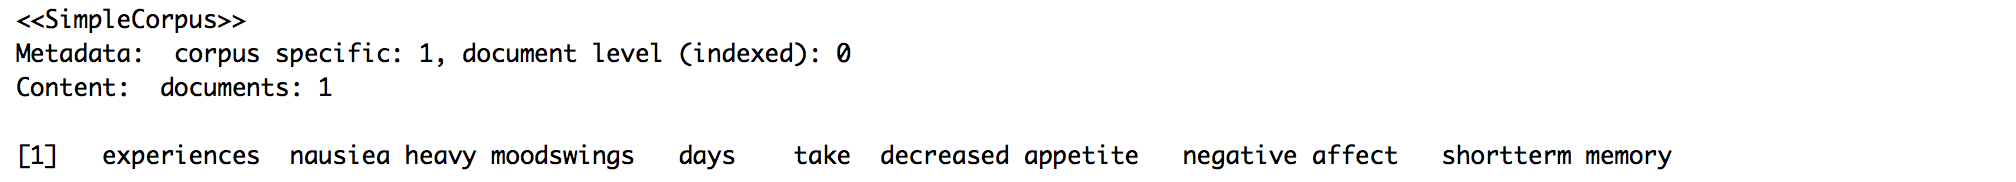
\includegraphics[width=1\textwidth]{imagenes/effects_stopwords.png}
    \caption{Contenido de effects sin stopwords}
    \label{benefits2}
\end{figure}

Ahora ya hemos eliminado las \emph{stopwords} de forma correcta, y
pasamos a realizar la agrupación de sinónimos.

\subsubsection{2.2.15. Agrupación de
sinónimos}\label{agrupacion-de-sinonimos}

Con el fin de disminuir la dimensión del espacio a trabajar, se pueden
identificar palabras distintas con el mismo significado y reemplazarlas
por una sola palabra. Para ello se toman los sinónimos de dicha palabra.
Dentro de las librerías que podemos usar para agrupar sinónimos,
destacamos dos: \texttt{wordnet} y \texttt{rword2vec}. Sin embargo, por
su sencillez se va hacer uso de \texttt{rword2vec}. Previamente, se
obtendrán qué palabras son las que mayor frecuencia presentan en nuestro
texto, tanto para \emph{benefitsReview} como \emph{sideEffectsReview}
del conjunto train y test.

Visualizamos los 4 primeros términos que cumplen estas características
para cada columna y conjunto train y test:

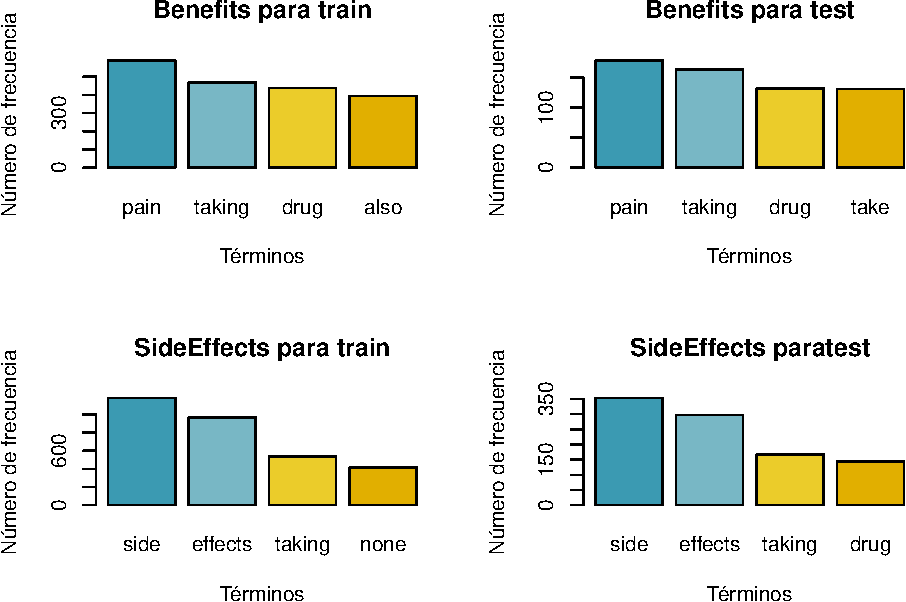
\includegraphics{practica-original_files/figure-latex/unnamed-chunk-41-1.pdf}

Una vez que tenemos los términos con mayor frecuencia en nuestras
columnas (\emph{benefitsReview} y \emph{sideEffectsReview}) y su
frecuencia asociada, pasamos a matriz dichos datos, con el fin de
obtener únicamente las palabras y descartar su frecuencia asociada.

Como ya sabemos las palabras a usar, es decir, los términos que más se
repiten, procedemos a la agrupación por sinónimos. En donde, mediante la
función \emph{distance(\ldots{})} de la librería \emph{rword2vec},
obtendremos todas palabras más similares de nuestro conjunto. En nuestro
caso nos vamos a quedar con las 2 primeras, tanto para
\emph{benefitsTrainReview} como \emph{sideEffectsReview} del conjunto
train y test. A continuación, se muestran los pasos seguidos.

\begin{enumerate}
\def\labelenumi{\arabic{enumi}.}
\tightlist
\item
  Escribir un fichero los datos asociados a dicha columna.
\item
  Entrenar los datos del fichero, con el fin de obtener los vectores de
  palabras que nos darán los palabras más similares.
\item
  Obtener para cada término del documento, la distancia con los térmios
  del ficheros, quedándonos con las de mayor frecuencia.
\item
  Guardar en un fichero dichas distancias.
\end{enumerate}

Una vez, que tenemos todas las palabras con los 2 términos más
similares, procedemos a sustituir todos esos términos por el término
general. Veamos un ejemplo sencillo, en donde las palabras ``medicine''
o ``medication'', van a ser sustituidas por ``drug''.

\begin{Shaded}
\begin{Highlighting}[]
\CommentTok{# Obtenemos el tercer término -> "drug"}
\NormalTok{terms_benefits_train_corpus[}\DecValTok{3}\NormalTok{]}
\end{Highlighting}
\end{Shaded}

\begin{verbatim}
## [1] "drug"
\end{verbatim}

\begin{Shaded}
\begin{Highlighting}[]
\CommentTok{# Vamos a sustituir "pain" por sus dos palabras más similares}
\NormalTok{dist_terms_benefits_train_corpus_new[[}\DecValTok{3}\NormalTok{]]}
\end{Highlighting}
\end{Shaded}

\begin{verbatim}
## [1] medication medicine  
## Levels: medication medicine
\end{verbatim}

Se debe tener en cuenta, que los términos más similares han sido creados
únicamente para nuestros documentos. Por último, ya solo nos queda hacer
el reemplazamiento, para ello se usará la función \emph{gsub(\ldots{})}
sobre el corpus (\emph{benefits\_corpus} y \emph{sideEffectsReview}).
Para sustituir las palabras en el texto, se ha hecho uso de la función
\texttt{gsub(pattern,\ replacement,\ x,\ ignore.case\ =\ FALSE,\ perl\ =\ FALSE,\ fixed\ =\ FALSE,\ useBytes\ =\ FALSE)}.
A continuación, se describe el proceso seguido:

\begin{enumerate}
\def\labelenumi{\arabic{enumi}.}
\tightlist
\item
  Iteramos sobre los términos del documento.
\item
  Iteramos sobre las palabras más frecuentes de cada término.
\item
  Realizamos el reemplazamiento de las palabras más similares por los
  términos generales, previa conversión a minúsculas.
\item
  Guardamos los resultados en ficheros.
\end{enumerate}

\subsubsection{2.2.16. TF-IDF}\label{tf-idf}

Para estudiar la importancia de los términos de un documento en
particular, en lugar de utilizar la frecuencia de cada uno de los
términos directamente, se pueden utilizar diferentes ponderaciones
denominadas TF-IDF (\emph{Term Frequency-Inverse Document Frecuency}).
Estas ponderaciones se calculan como el producto de dos medidas, la
frecuencia de aparición del término (\(tf\)) y la frecuencia inversa del
documento (\(idf\)). La fórmula matemática para esta métrica es la
siguiente:

\[ tfidf(t, d, D) = tf(t, d) × idf(t, D)\]

donde \(t\) es el término, \(d\) denota cada documento, \(D\) el espacio
total de documentos y \(tfidf\) es el peso asignado a ese término en el
documento correspondiente.

La combinación de los valores de \(tf\) e \(idf\) da una métrica que
permite saber cómo de únicas son las palabras de un documento. La
ponderación asigna un alto peso a un término si se produce con
frecuencia en ese documento, pero rara vez en la colección completa. Sin
embargo, si el término ocurre pocas veces en el documento, o aparece
prácticamente en todos ellos, disminuye el peso asignado por la
ponderación \(tfidf\). \textbf{De esta forma, obtenemos una forma de
asignar a cada término un score en relación a cuán representativo es
dicho término en nuestro conjunto de datos.}

El peso aumenta proporcionalmente al número de veces que una palabra
aparece en el documento, pero es compensada por la frecuencia de la
palabra en la colección de documentos, lo que permite filtrar las
palabras más comunes. Para ello, necesitamos que convertir nuestro
corpus a un \emph{dataframe}, en donde cada columna será una palabra del
comentario y cada fila un comentario.

\textbf{Frecuencia del término}

La primera parte de la fórmula \(tf(t, d)\) es simplemente calcular el
número de veces que aparece cada palabra en cada documento:

\begin{enumerate}
\def\labelenumi{\arabic{enumi}.}
\tightlist
\item
  Creamos el corpus utilizando el vector de string que hemos creado
  previamente.
\item
  Generamos la matriz de términos.
\item
  Convertimos a matriz.
\end{enumerate}

\textbf{Frecuencia inversa del documento}

Durante el cálculo de la frecuencia del término se considera que todos
los términos tienen igual importancia, no obstante, se conocen casos en
los que ciertos términos pueden aparecer muchas veces pero tienen poca
importancia. Esta segunda parte de la fórmula completa el análisis de
evaluación de los términos y actúa como corrector de \(tf\). Usando la
matriz de frecuencia de términos, el peso \(idf\) se puede calcular de
la siguiente forma:

\begin{Shaded}
\begin{Highlighting}[]
\CommentTok{# Calculamos los pesos asociados a cada término en train}
\NormalTok{terms_benefits_train <-}\StringTok{ }\NormalTok{( idf_benefits_train <-}\StringTok{ }\KeywordTok{log}\NormalTok{( }\KeywordTok{ncol}\NormalTok{(tf_benefits_train) }
                                                \OperatorTok{/}\StringTok{ }\NormalTok{( }\DecValTok{1}\OperatorTok{+}\KeywordTok{rowSums}\NormalTok{(tf_benefits_train }\OperatorTok{!=}\StringTok{ }\DecValTok{0}\NormalTok{))))}
\NormalTok{terms_effects_train <-}\StringTok{ }\NormalTok{( idf_effects_train <-}\StringTok{ }\KeywordTok{log}\NormalTok{( }\KeywordTok{ncol}\NormalTok{(tf_effects_train) }
                                                \OperatorTok{/}\StringTok{ }\NormalTok{( }\DecValTok{1}\OperatorTok{+}\KeywordTok{rowSums}\NormalTok{(tf_effects_train }\OperatorTok{!=}\StringTok{ }\DecValTok{0}\NormalTok{))))}

\CommentTok{# Calculamos los pesos asociados a cada término en test}
\NormalTok{terms_benefits_test <-}\StringTok{ }\NormalTok{( idf_benefits_test <-}\StringTok{ }\KeywordTok{log}\NormalTok{( }\KeywordTok{ncol}\NormalTok{(tf_benefits_test) }
                                                \OperatorTok{/}\StringTok{ }\NormalTok{( }\DecValTok{1}\OperatorTok{+}\KeywordTok{rowSums}\NormalTok{(tf_benefits_test }\OperatorTok{!=}\StringTok{ }\DecValTok{0}\NormalTok{))))}
\NormalTok{terms_effects_test <-}\StringTok{ }\NormalTok{( idf_effects_test <-}\StringTok{ }\KeywordTok{log}\NormalTok{( }\KeywordTok{ncol}\NormalTok{(tf_effects_test) }
                                               \OperatorTok{/}\StringTok{ }\NormalTok{( }\DecValTok{1}\OperatorTok{+}\KeywordTok{rowSums}\NormalTok{(tf_effects_test }\OperatorTok{!=}\StringTok{ }\DecValTok{0}\NormalTok{))))}

\CommentTok{# Muestra los pesos asociados a cada término (los 5 primeros)}
\NormalTok{terms_benefits_train[}\DecValTok{1}\OperatorTok{:}\DecValTok{5}\NormalTok{] }
\end{Highlighting}
\end{Shaded}

\begin{verbatim}
##      agents       alone  congestive dysfunction      failur 
##    6.941835    5.044715    6.654153    6.941835    7.347300
\end{verbatim}

Ahora que tenemos nuestra matriz con el término frecuencia y el peso
idf, estamos listos para calcular el peso total de \(tf-idf\). Para
hacer esta multiplicación de matrices, también tendremos que transformar
el vector \(idf\) en una matriz diagonal. Ambos cálculos se muestran a
continuación.

\begin{enumerate}
\def\labelenumi{\arabic{enumi}.}
\tightlist
\item
  Creamos la matriz diagonal:
  \texttt{(\ idf\_benefits\_train\ \textless{}-\ diag(idf\_benefits\_train)\ )}
\item
  Hacemos la operación para calcular \(tf_idf\) como el producto de
  \(td \cdot idf\):
  \texttt{tf\_idf\_benefits\_train\textless{}-\ crossprod(tf\_benefits\_train,\ idf\_benefits\_train)}
\item
  Guardamos los datos en ficheros, con el fin de reducir el tiempo de
  procesamiento.
\end{enumerate}

Hay que recordar que en la sección \(tf\) (frecuencia del término),
estamos representando cada término como el número de veces que
aparecieron en el documento. El principal problema para esta
representación es que creará un sesgo hacia documentos largos, ya que un
término dado tiene más posibilidades de aparecer en documentos más
largos, lo que los hace parecer más importantes de lo que realmente son.
Por lo tanto, el enfoque para resolver este problema es la
normalización:

\[ t\_benefits\_train = \frac{tf\_idf\_benefits\_train\_new}{\sqrt(rowSums( tf\_idf\_benefits\_train\_new^2 ) )}\]

A continuación, vamos a visualizar los términos que más se repiten para
el conjunto train de \emph{benefits}:

\begin{Shaded}
\begin{Highlighting}[]
\CommentTok{# Graficamos los resultados para benefits train}
\KeywordTok{ggplot}\NormalTok{() }\OperatorTok{+}\StringTok{ }
\StringTok{ }\KeywordTok{geom_bar}\NormalTok{(}\DataTypeTok{data=}\NormalTok{z_benefits_train[}\DecValTok{1}\OperatorTok{:}\DecValTok{10}\NormalTok{,],}
          \KeywordTok{aes}\NormalTok{(}\DataTypeTok{x=}\NormalTok{z_benefits_train}\OperatorTok{$}\NormalTok{terms1_5_new_benefits_train[}\DecValTok{1}\OperatorTok{:}\DecValTok{10}\NormalTok{],}
          \DataTypeTok{y=}\NormalTok{z_benefits_train}\OperatorTok{$}\NormalTok{v_benefits_train[}\DecValTok{1}\OperatorTok{:}\DecValTok{10}\NormalTok{]), }\DataTypeTok{stat=}\StringTok{'identity'}\NormalTok{, }
          \DataTypeTok{position=}\StringTok{'dodge'}\NormalTok{) }\OperatorTok{+}\StringTok{ }
\StringTok{  }\KeywordTok{ggtitle}\NormalTok{(}\StringTok{"Las 10 palabras que más se repiten con TFIDF"}\NormalTok{) }\OperatorTok{+}\StringTok{ }
\StringTok{  }\KeywordTok{xlab}\NormalTok{(}\StringTok{"Términos"}\NormalTok{) }\OperatorTok{+}
\StringTok{  }\KeywordTok{ylab}\NormalTok{(}\StringTok{"Frecuencia de los términos"}\NormalTok{)}
\end{Highlighting}
\end{Shaded}

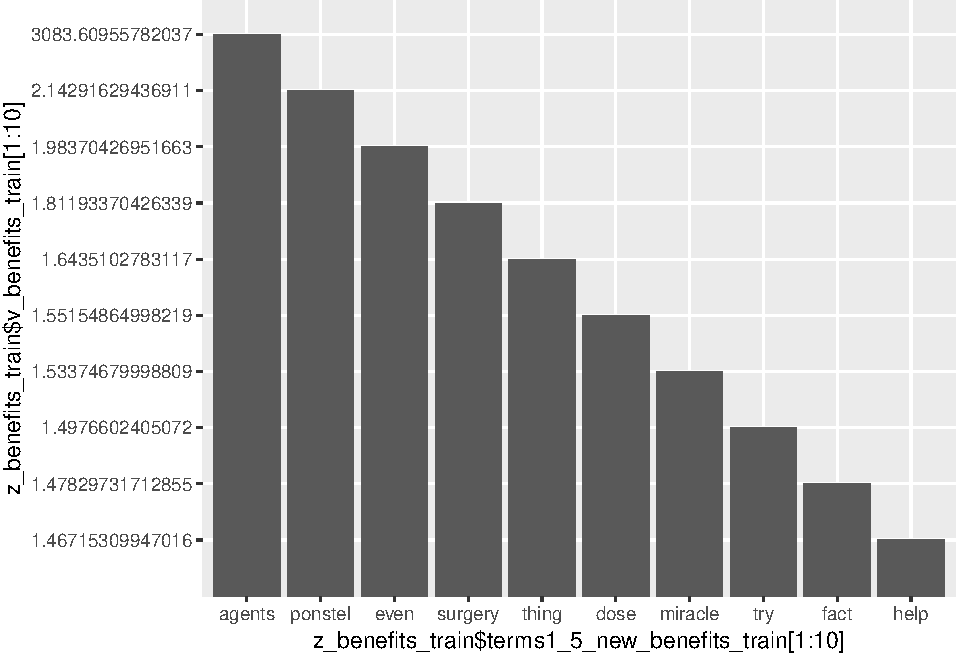
\includegraphics{practica-original_files/figure-latex/unnamed-chunk-60-1.pdf}

\subsubsection{2.2.17. Stemming}\label{stemming}

El siguiente paso consiste en reducir el número de palabras totales con
las que estamos trabajando. En este caso, se trata de reducir aquellas
que no nos aportan nada relevante a lo que ya tenemos. Por ejemplo, en
este dataframe se repite una gran cantidad de veces la palabra
``benefit'', al igual que ``benefits''. Sin embargo, realizar el
análisis de nuestros datos con ambas palabras no tiene gran relevancia,
ya que una no aporta nada respecto a la otra. Este es un ejemplo del
tipo de casos que se nos dan en nuestro dataset.

Igual ocurre con ``reduce'' y ``reduced'', por ejemplo. Este tipo de
situaciones son las que intentamos corregir con este paso. Vamos a ver
un ejemplo de este suceso, que se da por ejemplo en los siguientes
valores del corpus (y en muchos más).

\begin{Shaded}
\begin{Highlighting}[]
\KeywordTok{inspect}\NormalTok{(benefits_train_corpus_new_load[}\DecValTok{183}\NormalTok{])}
\end{Highlighting}
\end{Shaded}

\begin{verbatim}
## <<SimpleCorpus>>
## Metadata:  corpus specific: 1, document level (indexed): 0
## Content:  documents: 1
## 
## [1]  treatment benefits   temporary    made sneezing  watery eyes diminish    address  issue  respiratory difficulties   found   may  even increased  respiratory symptoms   process
\end{verbatim}

\begin{Shaded}
\begin{Highlighting}[]
\KeywordTok{inspect}\NormalTok{(benefits_train_corpus_new_load[}\DecValTok{213}\NormalTok{])}
\end{Highlighting}
\end{Shaded}

\begin{verbatim}
## <<SimpleCorpus>>
## Metadata:  corpus specific: 1, document level (indexed): 0
## Content:  documents: 1
## 
## [1] overall   ease mantally    true benefit  felt
\end{verbatim}

A continuación, aplicamos el proceso de stemming mediante la siguiente
función:

\begin{Shaded}
\begin{Highlighting}[]
\NormalTok{benefits_train_corpus_new_load <-}\StringTok{ }\KeywordTok{tm_map}\NormalTok{(benefits_train_corpus_new_load, stemDocument)}
\NormalTok{effects_train_corpus_new_load <-}\StringTok{ }\KeywordTok{tm_map}\NormalTok{(effects_train_corpus_new_load, stemDocument)}

\NormalTok{benefits_test_corpus_new_load <-}\StringTok{ }\KeywordTok{tm_map}\NormalTok{(benefits_test_corpus_new_load, stemDocument)}
\NormalTok{effects_test_corpus_new_load <-}\StringTok{ }\KeywordTok{tm_map}\NormalTok{(effects_test_corpus_new_load, stemDocument)}
\end{Highlighting}
\end{Shaded}

Si ahora volvemos a mostrar el contenido de dichas opiniones, podemos
ver que el cambio se ha hecho efectivo: donde ponía \textit{benefits},
ahora pone \textit{benefit}, como se puede comprobar si volvemos a
mostrar dichos elementos del corpus. De hecho, si nos fijamos, no solo
esta palabra ha resultado modificada, sino que se han resumido muchas
más palabras en comparación a como teníamos los documentos en el momento
previo a la aplicación del método \textit{Stem}. Desde este momento, ya
tenemos nuestro conjunto reducido a nivel de concepto.

\begin{Shaded}
\begin{Highlighting}[]
\KeywordTok{inspect}\NormalTok{(benefits_train_corpus_new_load[}\DecValTok{183}\NormalTok{])}
\end{Highlighting}
\end{Shaded}

\begin{verbatim}
## <<SimpleCorpus>>
## Metadata:  corpus specific: 1, document level (indexed): 0
## Content:  documents: 1
## 
## [1] treatment benefit temporari made sneez wateri eye diminish address issu respiratori difficulti found may even increas respiratori symptom process
\end{verbatim}

\begin{Shaded}
\begin{Highlighting}[]
\KeywordTok{inspect}\NormalTok{(benefits_train_corpus_new_load[}\DecValTok{213}\NormalTok{])}
\end{Highlighting}
\end{Shaded}

\begin{verbatim}
## <<SimpleCorpus>>
## Metadata:  corpus specific: 1, document level (indexed): 0
## Content:  documents: 1
## 
## [1] overal eas mantal true benefit felt
\end{verbatim}

\subsubsection{2.2.18. Valores perdidos}\label{valores-perdidos}

Tras el proceso de limpieza anterior en un volumen tan grande de datos
cabe esperar que algún documento estuviera formado por tan solo palabras
vacías, enlaces o combinaciones de estos, es por ello, que por medio de
filtrado básico de R se obtienen aquellos que no contienen ninguna
palabra y se elimina del conjunto del dataset para evitar problemas en
los procesos posteriores.

\begin{Shaded}
\begin{Highlighting}[]
\CommentTok{# https://github.com/joseangeldiazg/twitter-text-mining/blob/master/ner.R}
\CommentTok{# Localizamos posibles valores perdidos que se hayan generado tras el proceso de limpieza}
\KeywordTok{which}\NormalTok{(benefits_train_corpus_new_load}\OperatorTok{$}\NormalTok{content}\OperatorTok{==}\StringTok{""}\NormalTok{)}
\KeywordTok{which}\NormalTok{(effects_train_corpus_new_load}\OperatorTok{$}\NormalTok{content}\OperatorTok{==}\StringTok{" "}\NormalTok{)}
\KeywordTok{which}\NormalTok{(benefits_test_corpus_new_load}\OperatorTok{$}\NormalTok{content}\OperatorTok{==}\StringTok{"  "}\NormalTok{)}
\KeywordTok{which}\NormalTok{(effects_test_corpus_new_load}\OperatorTok{$}\NormalTok{content}\OperatorTok{==}\StringTok{"   "}\NormalTok{)}

\CommentTok{# Vemos que no hay muchos vacios }
\NormalTok{benefits_train_corpus_new_load<-benefits_train_corpus_new_load[}
  \KeywordTok{which}\NormalTok{(benefits_train_corpus_new_load}\OperatorTok{$}\NormalTok{content}\OperatorTok{!=}\StringTok{""}\NormalTok{)]}
\NormalTok{effects_train_corpus_new_load<-effects_train_corpus_new_load[}
  \KeywordTok{which}\NormalTok{(effects_train_corpus_new_load}\OperatorTok{$}\NormalTok{content}\OperatorTok{!=}\StringTok{" "}\NormalTok{)]}
\NormalTok{benefits_test_corpus_new_load<-benefits_test_corpus_new_load[}
  \KeywordTok{which}\NormalTok{(benefits_test_corpus_new_load}\OperatorTok{$}\NormalTok{content}\OperatorTok{!=}\StringTok{"  "}\NormalTok{)]}
\NormalTok{effects_test_corpus_new_load<-effects_test_corpus_new_load[}
  \KeywordTok{which}\NormalTok{(effects_test_corpus_new_load}\OperatorTok{$}\NormalTok{content}\OperatorTok{!=}\StringTok{"   "}\NormalTok{)]}
\end{Highlighting}
\end{Shaded}

\subsubsection{2.2.19. Borrar espacios en blanco
innecesarios}\label{borrar-espacios-en-blanco-innecesarios}

Hasta el momento hemos hecho distintos cambios en el texto de nuestro
dataset. No solo hemos modificado algunas palabras, sino que también
hemos borrado otras muchas. Por ello, es adecuado asegurarnos de que no
hay más espacios en blanco que los que separan las palabras del texto.
Para asegurarnos de ello, podemos ejecutar la siguiente orden, que se
encarga de suprimir los espacios en blanco sobrantes.

\begin{Shaded}
\begin{Highlighting}[]
\NormalTok{benefits_train_corpus_new_load <-}\StringTok{ }\KeywordTok{tm_map}\NormalTok{(benefits_train_corpus_new_load, stripWhitespace) }
\NormalTok{effects_train_corpus_new_load <-}\StringTok{ }\KeywordTok{tm_map}\NormalTok{(effects_train_corpus_new_load, stripWhitespace) }

\NormalTok{benefits_test_corpus_new_load <-}\StringTok{ }\KeywordTok{tm_map}\NormalTok{(benefits_test_corpus_new_load, stripWhitespace) }
\NormalTok{effects_test_corpus_new_load <-}\StringTok{ }\KeywordTok{tm_map}\NormalTok{(effects_test_corpus_new_load, stripWhitespace) }
\end{Highlighting}
\end{Shaded}

\subsubsection{2.2.20. Sparsity}\label{sparsity}

También puede resultar muy útil eliminar los términos que aparecen en
muy pocos documentos antes de proceder a la clasificación. El motivo
principal es la factibilidad computacional, ya que este proceso reduce
drásticamente el tamaño de la matriz sin perder información
significativa. Además puede eliminar errores en los datos, como podrían
ser palabras mal escritas, o simplemente borrar las palabras que
aparezcan una única vez en el dataframe, y que difícilmente nos
aportarán información relevante que podamos extrapolar. Para suprimir
estos términos, denominados escasos, se utiliza el comando
\texttt{removeSparseTerms()}.

\[ df(t) > N \cdot (1 != sparse)\] siendo \(df\) la frecuencia de
documentos del término \(t\) y \(N\) el número de vectores. El parámetro
\emph{sparse} toma valores entre 0 y 1. En este caso, el umbral de
escasez es 0.999. Este umbral elegido significa que se toman los
términos que aparecen en más del 1\% de documentos.

\begin{Shaded}
\begin{Highlighting}[]
\NormalTok{dtm <-}\StringTok{ }\KeywordTok{DocumentTermMatrix}\NormalTok{(benefits_train_corpus_new_load)}
\KeywordTok{inspect}\NormalTok{(dtm)}
\end{Highlighting}
\end{Shaded}

\begin{verbatim}
## <<DocumentTermMatrix (documents: 3104, terms: 5835)>>
## Non-/sparse entries: 52316/18059524
## Sparsity           : 100%
## Maximal term length: 33
## Weighting          : term frequency (tf)
## Sample             :
##       Terms
## Docs   day drug effect feel help medic pain take time work
##   1049   4    0      0    0    0     0    5    1    1    1
##   1189   4    0      0    0    0     0    5    1    1    1
##   1279   0    0      1    3    2     0    0    1    1    1
##   1824   1    0      0    3    1     0    0    1    2    0
##   2504   4    1      3    0    1     4    0    2    0    3
##   317    7    2      0    1    1     1    0    3    4    0
##   339    1    1      5    1    2     6    0    2    0    1
##   462    4    1      3    0    1     4    0    2    0    3
##   565    3    2      2    3    0     0    6    4    0    1
##   665    3    4      0    3    0     0    0    1    1    0
\end{verbatim}

\begin{Shaded}
\begin{Highlighting}[]
\NormalTok{dtm <-}\StringTok{ }\KeywordTok{removeSparseTerms}\NormalTok{(dtm, }\DataTypeTok{sparse=}\FloatTok{0.999}\NormalTok{)}
\KeywordTok{inspect}\NormalTok{(dtm)}
\end{Highlighting}
\end{Shaded}

\begin{verbatim}
## <<DocumentTermMatrix (documents: 3104, terms: 1702)>>
## Non-/sparse entries: 46811/5236197
## Sparsity           : 99%
## Maximal term length: 17
## Weighting          : term frequency (tf)
## Sample             :
##       Terms
## Docs   day drug effect feel help medic pain take time work
##   1049   4    0      0    0    0     0    5    1    1    1
##   1189   4    0      0    0    0     0    5    1    1    1
##   1279   0    0      1    3    2     0    0    1    1    1
##   1824   1    0      0    3    1     0    0    1    2    0
##   2504   4    1      3    0    1     4    0    2    0    3
##   317    7    2      0    1    1     1    0    3    4    0
##   339    1    1      5    1    2     6    0    2    0    1
##   462    4    1      3    0    1     4    0    2    0    3
##   565    3    2      2    3    0     0    6    4    0    1
##   665    3    4      0    3    0     0    0    1    1    0
\end{verbatim}

Se observa como de 5835 términos pasamos a 1702 términos, por tanto se
ha considerado despreciar aplicar esta técnica ya que consideramos que
se ha perdido una gran cantidad de información, y, desde nuestro punto
de vista, creemos que no serían suficientes datos como para poder
aplicar las técnicas y obtener buenos resultados. Por ello, necesitamos
de estos los datos para la aplicación de las técnicas posteriores.

Luego, en función de la técnica que se aplique, si fuera necesario se
reducirá la dimensionalidad. En definitiva, ya tenemos nuestros datos
listos.

\subsubsection{2.2.21. Matriz de documentos de los
términos}\label{matriz-de-documentos-de-los-terminos}

Ahora vamos a mapear nuestro corpus creando una matriz de términos,
donde las filas corresponden a los documentos, las columnas a los
términos y cada casilla la ocurrencia de dicho término en dicho
documento. Para ello usaremos la función TermDocumentMatrix:

\begin{Shaded}
\begin{Highlighting}[]
\NormalTok{matrix_corpus <-}\StringTok{ }\KeywordTok{TermDocumentMatrix}\NormalTok{(benefits_train_corpus_new_load)}
\end{Highlighting}
\end{Shaded}

Podemos observar que tenemos 5838 términos, esto quiere decir que
tenemos 5838 palabras diferentes en nuestro Corpus. Obtengamos la
\emph{frecuencia de las palabras}:

Como podemos ver, actualmente aún no tenemos nuestros datos en la matriz
que buscamos, sino en un vector, por tanto:

Con este método, hemos obtenido la ocurrencia de las palabras que
tenemos en nuestro dataset para cada uno de los documentos/comentarios.
Esta matriz tiene 5838 columnas, que representa la totalidad de palabras
diferentes que hay en los comentarios de la columna
\textit{benefitsReview}, y 3107 filas, donde cada una representa un
comentario. Por tanto, en la fila iésima la matriz, tendremos la
ocurrencia de las palabras en \textit{benefitsReview} que existen en el
comentario \textit{i}.

\begin{Shaded}
\begin{Highlighting}[]
\CommentTok{# Sumamos las filas}
\NormalTok{suma_matrix_corpus <-}\StringTok{ }\KeywordTok{rowSums}\NormalTok{(matrix_corpus)}
\KeywordTok{head}\NormalTok{(suma_matrix_corpus,}\DecValTok{5}\NormalTok{)}
\end{Highlighting}
\end{Shaded}

\begin{verbatim}
##    agent     alon  congest dysfunct   failur 
##        2       19       19        2        7
\end{verbatim}

\begin{Shaded}
\begin{Highlighting}[]
\CommentTok{# Ordenamos de mayor a menor y muestra los 10 primeros}
\NormalTok{ordena_mayor_matrix_corpus <-}\StringTok{ }\KeywordTok{sort}\NormalTok{(suma_matrix_corpus, }\DataTypeTok{decreasing =} \OtherTok{TRUE}\NormalTok{)}
\KeywordTok{head}\NormalTok{(ordena_mayor_matrix_corpus,}\DecValTok{10}\NormalTok{)}
\end{Highlighting}
\end{Shaded}

\begin{verbatim}
##   take effect   pain    day   help   drug   feel   time   work  medic 
##    789    682    642    626    524    498    479    450    404    399
\end{verbatim}

\begin{Shaded}
\begin{Highlighting}[]
\NormalTok{copia_ordena_mayor =}\StringTok{ }\NormalTok{ordena_mayor_matrix_corpus }\CommentTok{# Para graficos (evitando data.frame)}

\CommentTok{# Ordenamos de menor a mayor y muestra los 10 primeros}
\NormalTok{ordena_menor_matrix_corpus <-}\StringTok{ }\KeywordTok{sort}\NormalTok{(suma_matrix_corpus, }\DataTypeTok{decreasing =} \OtherTok{FALSE}\NormalTok{)}
\KeywordTok{head}\NormalTok{(ordena_menor_matrix_corpus,}\DecValTok{10}\NormalTok{)}
\end{Highlighting}
\end{Shaded}

\begin{verbatim}
##         mangag          overt    ventricular            con           pros 
##              1              1              1              1              1 
##        ponstel          frank       valerian allergiesirrit          dryer 
##              1              1              1              1              1
\end{verbatim}

\begin{Shaded}
\begin{Highlighting}[]
\CommentTok{# Transformamos a objeto data.frame, con dos columnas (palabra, frec), }
\CommentTok{#para posteriormente graficarlo.}
\NormalTok{ordena_mayor_matrix_corpus <-}\StringTok{ }\KeywordTok{data.frame}\NormalTok{(}\DataTypeTok{palabra =} \KeywordTok{names}\NormalTok{(ordena_mayor_matrix_corpus), }
                                         \DataTypeTok{frec =}\NormalTok{ ordena_mayor_matrix_corpus)}
\end{Highlighting}
\end{Shaded}

Mostramos las más frecuentes:

\begin{Shaded}
\begin{Highlighting}[]
\NormalTok{ordena_mayor_matrix_corpus[}\DecValTok{1}\OperatorTok{:}\DecValTok{20}\NormalTok{,]}
\end{Highlighting}
\end{Shaded}

\begin{verbatim}
##             palabra frec
## take           take  789
## effect       effect  682
## pain           pain  642
## day             day  626
## help           help  524
## drug           drug  498
## feel           feel  479
## time           time  450
## work           work  404
## medic         medic  399
## also           also  394
## use             use  381
## sleep         sleep  381
## reduc         reduc  381
## year           year  369
## get             get  368
## skin           skin  358
## treatment treatment  357
## benefit     benefit  353
## depress     depress  349
\end{verbatim}

Y obtenemos la \emph{gráfica}:

\begin{Shaded}
\begin{Highlighting}[]
\NormalTok{copia_ordena_mayor <-}\StringTok{ }\KeywordTok{as.matrix}\NormalTok{(copia_ordena_mayor)}
\KeywordTok{barplot}\NormalTok{(copia_ordena_mayor[}\DecValTok{1}\OperatorTok{:}\DecValTok{10}\NormalTok{,],  }\DataTypeTok{xlab=}\StringTok{"Palabras"}\NormalTok{, }\DataTypeTok{ylab=}\StringTok{"Número de frecuencia"}\NormalTok{,}
        \DataTypeTok{col =} \KeywordTok{c}\NormalTok{(}\StringTok{"lightblue"}\NormalTok{, }\StringTok{"mistyrose"}\NormalTok{, }\StringTok{"lightcyan"}\NormalTok{,}
                \StringTok{"lavender"}\NormalTok{, }\StringTok{"cornsilk"}\NormalTok{))}
\KeywordTok{title}\NormalTok{(}\DataTypeTok{main =} \KeywordTok{list}\NormalTok{(}\StringTok{"Las nueve palabras más frecuentes después del preprocesamiento"}\NormalTok{, }\DataTypeTok{font =} \DecValTok{4}\NormalTok{))}
\end{Highlighting}
\end{Shaded}

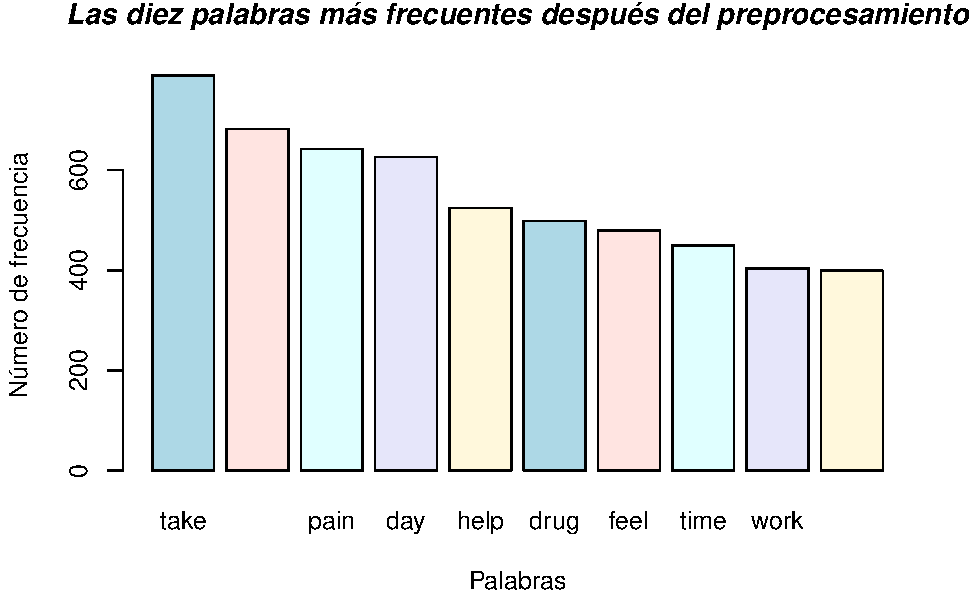
\includegraphics{practica-original_files/figure-latex/unnamed-chunk-74-1.pdf}

\subsubsection{2.2.22. Nube de palabras}\label{nube-de-palabras}

Por último, vamos a visualizar la nube de palabras para benefits
preprocesado, tanto al principio del procesamiento como al final. En
este caso, en vez de determinar los colores de las palabras en función
de la ocurrencia de éstos en el dataset, hemos aplicado la nube de
palabras de la forma que vimos en clase: \textbf{incluyendo análisis de
sentimientos}. Por ello, en primer lugar, identificaremos las palabras a
pintar como positivas o negativas, y posteriormente, se generará la nube
de palabras con las siguientes características: - Si la palabra tiene
una connotación positiva, aparecerá de color verde. - Si la palabra
tiene una connotación negativa, aparecerá de color rojo.

Este análisis es realmente determinante en nuestro problema, puesto que
al fin y al cabo, tenemos comentarios de pacientes, que estarán
orientados a una buena y positiva opinión del fármaco o al contrario
(una mala, y posiblemente molesta opinión acerca del mismo).

En este caso, visualizando la nube de palabras, obtenemos una cosa
clara: principalmente tenemos palabras de connotación negativa, aspecto
totalmente lógico puesto que, es más común que un usuario comente algo
para quejarse o mostrar su mala experiencia, que para hablar bien del
mismo. Además, al tratarse de temas de enfermedades y problemas de
salud, es mucho más fácil encontrar palabras relacionadas con el dolor,
o la preocupación, que con la alegría u otros aspectos derivados de las
connotaciones positivas.

\begin{figure}[h]
    \centering
    
\includegraphics[width=0.5\textwidth]{imagenes/wordcloud1.png}
    \caption{Wordcloud con preprocesamiento}
    \label{benefits2}
\end{figure}

\begin{figure}[h]
    \centering
    
\includegraphics[width=0.5\textwidth]{imagenes/wordcloud2.png}
    \caption{Wordcloud sin preprcesamiento}
    \label{benefits2}
\end{figure}

\subsection{2.2.23. Convertir a dataframe nuestras
modificaciones}\label{convertir-a-dataframe-nuestras-modificaciones}

Por último, con el fin de mejorar los tiempos computacionales y poder
hacer uso todos los integrantes del grupo de las columnas preprocesadas,
se ha optado por añadir dichos cambios en el dataset y guardarlos en un
fichero.

\textbf{\emph{Nota: Cuando se necesite en las sucesivas técnicas, se
realizarán las transformaciones necesarias de acuerdo a cada técnica en
cuestión.}}

\newpage

\section{3. Análisis exploratorio de los
datos}\label{analisis-exploratorio-de-los-datos}

El análisis exploratorio de datos o (EDA) engloba un conjunto de
técnicas para poder comprender de manera rápida la naturaleza de una
colección de datos o dataset. Se basa principalmente en dos criterios:
las \textbf{estadísticas de resumen} y la \textbf{visualización de
datos}.

En primer lugar, vamos a realizar un resumen de nuestros datos
utilizando la función \texttt{summary()}. Dicha función nos mostrará
información relevante para cada una de las columnas del datataset,
mostrando información general como valores mínimos, máximos, media,
mediana. El resultado que obtenemos al evaluar nuestro dataset es el
siguiente:

\begin{Shaded}
\begin{Highlighting}[]
\KeywordTok{summary}\NormalTok{(datos_train)}
\end{Highlighting}
\end{Shaded}

\begin{verbatim}
##    urlDrugName       rating                      effectiveness 
##  lexapro :  63   Min.   : 1.000   Considerably Effective: 926  
##  prozac  :  46   1st Qu.: 5.000   Highly Effective      :1330  
##  retin-a :  45   Median : 8.000   Ineffective           : 247  
##  zoloft  :  45   Mean   : 7.008   Marginally Effective  : 186  
##  paxil   :  38   3rd Qu.: 9.000   Moderately Effective  : 415  
##  propecia:  38   Max.   :10.000                                
##  (Other) :2829                                                 
##                         sideEffects                 condition   
##  Extremely Severe Side Effects: 175   depression         : 236  
##  Mild Side Effects            :1019   acne               : 165  
##  Moderate Side Effects        : 612   anxiety            :  63  
##  No Side Effects              : 930   insomnia           :  54  
##  Severe Side Effects          : 368   birth control      :  49  
##                                       high blood pressure:  42  
##                                       (Other)            :2495  
##                                                                                                                                                                                                                                                                                                                          benefitsReview
##  none                                                                                                                                                                                                                                                                                                                           :  20  
##  None                                                                                                                                                                                                                                                                                                                           :  18  
##  NONE                                                                                                                                                                                                                                                                                                                           :   3  
##  None.                                                                                                                                                                                                                                                                                                                          :   3  
##  The treatment benefits were marginal at best.  Mood neither improved nor deteriorated, and anxiety was never significantly alleviated.  Unsurprisingly, recent research suggests that SSRIs are only effective in the most severe of cases.                                                                                    :   3  
##  Before the use of vagifem tablets, I had to endure a series of urinary infections after sometimes painful sexual intercourse.  I also had painful cracks in mucoal lining of vulva due to aging and dryness.  After beginning the use of this drug, I found that the ncreased mucous in vagina resolved both of these problems.:   2  
##  (Other)                                                                                                                                                                                                                                                                                                                        :3055  
##                    sideEffectsReview sideEffectsNumber effectivenessNumber
##  none                       : 112    Min.   :1.000     Min.   :1.000      
##  None                       :  73    1st Qu.:1.000     1st Qu.:3.000      
##  None.                      :  19    Median :2.000     Median :4.000      
##  No side effects.           :   9    Mean   :2.304     Mean   :3.936      
##  There were no side effects.:   6    3rd Qu.:3.000     3rd Qu.:5.000      
##  no side effects            :   5    Max.   :5.000     Max.   :5.000      
##  (Other)                    :2880                                         
##  weightedRating    ratingLabel     sideEffectsInverse
##  Min.   : 2.000   Min.   :0.0000   Min.   :1.000     
##  1st Qu.: 6.000   1st Qu.:1.0000   1st Qu.:3.000     
##  Median : 8.000   Median :1.0000   Median :4.000     
##  Mean   : 7.737   Mean   :0.7874   Mean   :3.696     
##  3rd Qu.:10.000   3rd Qu.:1.0000   3rd Qu.:5.000     
##  Max.   :10.000   Max.   :1.0000   Max.   :5.000     
##                                                      
##                                                                                                                                           benefits_preprocesado
##  none                                                                                                                                                :  50     
##  lower blood pressur                                                                                                                                 :   7     
##  prevent pregnanc                                                                                                                                    :   3     
##  treatment benefit margin best mood neither improv deterior anxieti never signific allevi unsurpris recent research suggest ssris effect sever case  :   3     
##  abl work without hassl im free pain right now there need cri anymor whenev urin                                                                     :   2     
##  believ multipl treatment benefit take tylenol headach tylenol safe inexpens requir physician prescript addit avail almost everywher therefor conveni:   2     
##  (Other)                                                                                                                                             :3037     
##         effects_preprocesado
##  none             : 214     
##  side effect      :  51     
##  none notic       :  17     
##  none awar        :   8     
##  notic side effect:   7     
##  none can tell    :   6     
##  (Other)          :2801
\end{verbatim}

A continuación se va a realizar un análisis de la información más
relevante no textual, como el valor de \textbf{rating} de los usuarios,
la \textbf{efectividad} y los \textbf{efectos secundarios} de dicho
medicamento y por último, la \textbf{valoración ponderada del rating}
teniendo en cuenta la proporción entre efectividad y efectos secundarios
del medicamento.

\subsection{3.1. Valoraciones de los medicamentos por parte de los
usuarios.}\label{valoraciones-de-los-medicamentos-por-parte-de-los-usuarios.}

En primer lugar vamos a analizar si el \emph{rating} aportado por los
usuarios sobre los medicamentos es, en general, bueno o no. Para ello
empezamos obteniendo las frecuencias y porcentaje total de las
valoraciones aportadas por los usuarios. Por tanto, se va a calcular la
frecuencia de dicho atributo y su porcentaje respecto del total.

\begin{Shaded}
\begin{Highlighting}[]
\CommentTok{# Obtener frecuencias del rating}
\KeywordTok{table}\NormalTok{(datos_train}\OperatorTok{$}\NormalTok{rating)}
\end{Highlighting}
\end{Shaded}

\begin{verbatim}
## 
##   1   2   3   4   5   6   7   8   9  10 
## 305 102 146 107 158 157 349 558 480 742
\end{verbatim}

\begin{Shaded}
\begin{Highlighting}[]
\CommentTok{# Calculamos el número de documentos}
\NormalTok{numDocuments <-}\StringTok{ }\KeywordTok{dim}\NormalTok{(datos_train)[}\DecValTok{1}\NormalTok{]}

\CommentTok{# Calculamos el porcentaje de cada puntuación respecto del total.}
\KeywordTok{table}\NormalTok{(datos_train}\OperatorTok{$}\NormalTok{rating)}\OperatorTok{/}\NormalTok{numDocuments}
\end{Highlighting}
\end{Shaded}

\begin{verbatim}
## 
##          1          2          3          4          5          6 
## 0.09826031 0.03286082 0.04703608 0.03447165 0.05090206 0.05057990 
##          7          8          9         10 
## 0.11243557 0.17976804 0.15463918 0.23904639
\end{verbatim}

Como podemos observar, hay una mayoría de valoraciones positivas
respecto a las negativas. De hecho el mayor porcentaje (casi el 24\%)
tienen la máxima valoración. Podemos comprobar ésto mediante el uso de
la moda.

\begin{Shaded}
\begin{Highlighting}[]
\CommentTok{# Función para calcular la moda. Se le pasa como parámetro un atributo}
\NormalTok{calcularModa<-}\ControlFlowTok{function}\NormalTok{(var)\{}
\NormalTok{  frec.var<-}\KeywordTok{table}\NormalTok{(var)}
\NormalTok{  valor<-}\KeywordTok{which}\NormalTok{(frec.var}\OperatorTok{==}\KeywordTok{max}\NormalTok{(frec.var))  }\CommentTok{# Elementos con el valor m}
  \KeywordTok{names}\NormalTok{(valor)}
\NormalTok{\}}

\CommentTok{# Obtenemos la moda para el rating}
\KeywordTok{calcularModa}\NormalTok{(datos_train}\OperatorTok{$}\NormalTok{rating)}
\end{Highlighting}
\end{Shaded}

\begin{verbatim}
## [1] "10"
\end{verbatim}

Como resumen en general del rating, se va a calcular la media y la
mediana para calcular la tendencia central para dicha variable. La media
es la siguiente:

\begin{Shaded}
\begin{Highlighting}[]
\CommentTok{# Media}
\KeywordTok{mean}\NormalTok{(datos_train}\OperatorTok{$}\NormalTok{rating)}
\end{Highlighting}
\end{Shaded}

\begin{verbatim}
## [1] 7.008376
\end{verbatim}

La mediana es la siguiente:

\begin{Shaded}
\begin{Highlighting}[]
\CommentTok{# Mediana}
\KeywordTok{median}\NormalTok{(datos_train}\OperatorTok{$}\NormalTok{rating)}
\end{Highlighting}
\end{Shaded}

\begin{verbatim}
## [1] 8
\end{verbatim}

El valor medio obtenido es 7 y la mediana es 8. Podemos concluir con
dicha información, que en general las valoraciones sobre los
medicamentos son bastante positivas, situándose el 50\% de dichas
valoraciones en el valor 8.

A continuación, se va a visualizar dicha información gráficamente:

\begin{Shaded}
\begin{Highlighting}[]
\CommentTok{# Histograma de la valoración dada por los usuarios sobre los medicamentos}
\NormalTok{ratingExploration <-}\StringTok{ }\NormalTok{datos_train}\OperatorTok{$}\NormalTok{rating}

\KeywordTok{hist}\NormalTok{(ratingExploration,}
     \DataTypeTok{main=}\StringTok{"Rating de los medicamentos"}\NormalTok{,}
     \DataTypeTok{xlab=}\StringTok{"Rating"}\NormalTok{,}
     \DataTypeTok{ylab=}\StringTok{"Frecuencia"}\NormalTok{,}
     \DataTypeTok{border=}\StringTok{"goldenrod3"}\NormalTok{,}
     \DataTypeTok{xlim=}\KeywordTok{c}\NormalTok{(}\DecValTok{0}\NormalTok{,}\DecValTok{10}\NormalTok{),}
     \DataTypeTok{ylim=}\KeywordTok{c}\NormalTok{(}\DecValTok{0}\NormalTok{,}\DecValTok{800}\NormalTok{),}
     \DataTypeTok{col=} \StringTok{"cornsilk"}\NormalTok{,}
     \DataTypeTok{breaks=}\DecValTok{10}\NormalTok{,)}
\end{Highlighting}
\end{Shaded}

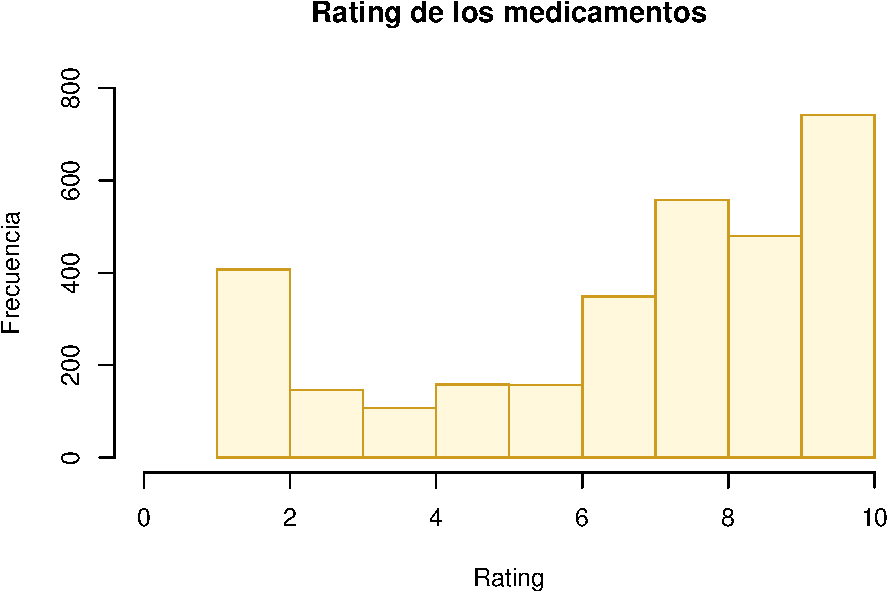
\includegraphics{practica-original_files/figure-latex/unnamed-chunk-84-1.pdf}

\begin{Shaded}
\begin{Highlighting}[]
\CommentTok{# Diagrama de densidad de la valoración dada por los usuarios sobre los medicamentos}
\KeywordTok{plot}\NormalTok{(}\KeywordTok{density}\NormalTok{(ratingExploration), }
     \DataTypeTok{main=}\StringTok{"Densidad del rating"}\NormalTok{,}
     \DataTypeTok{xlim=}\KeywordTok{c}\NormalTok{(}\DecValTok{0}\NormalTok{,}\DecValTok{10}\NormalTok{),}
\NormalTok{     )}
\end{Highlighting}
\end{Shaded}

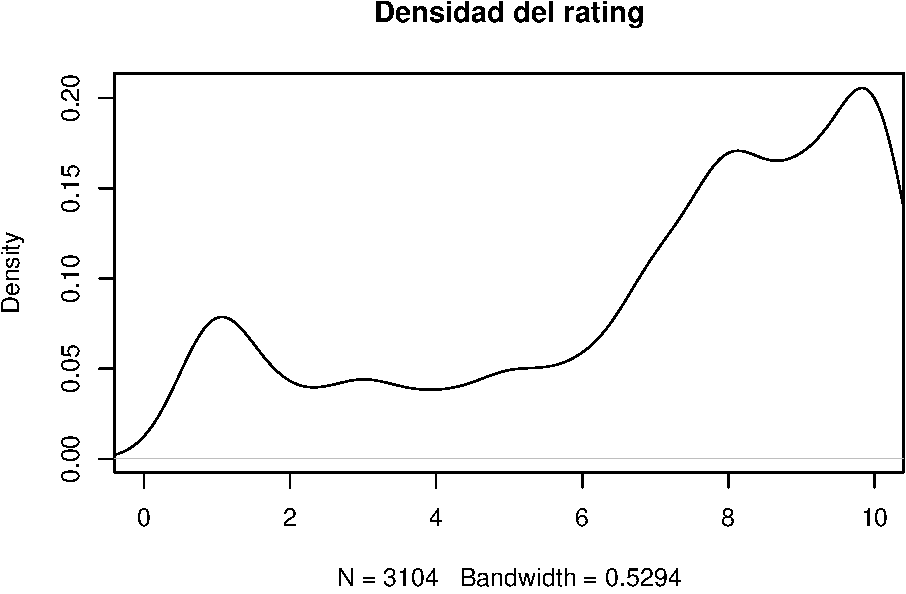
\includegraphics{practica-original_files/figure-latex/unnamed-chunk-85-1.pdf}

\begin{Shaded}
\begin{Highlighting}[]
\CommentTok{# Diagrama de sectores de las valoraciones dadas por los usuarios}
\KeywordTok{pie}\NormalTok{(}\KeywordTok{table}\NormalTok{(datos_train}\OperatorTok{$}\NormalTok{rating))}
\end{Highlighting}
\end{Shaded}

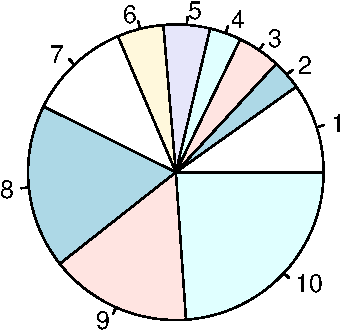
\includegraphics{practica-original_files/figure-latex/unnamed-chunk-86-1.pdf}

\begin{Shaded}
\begin{Highlighting}[]
\CommentTok{# Diagrama de cajas sobre las valoraciones dadas por los usuarios}
\KeywordTok{boxplot}\NormalTok{(datos_train}\OperatorTok{$}\NormalTok{rating,}\DataTypeTok{main=}\StringTok{"Rating"}\NormalTok{, }\DataTypeTok{col=} \StringTok{"cornsilk"}\NormalTok{ )}
\end{Highlighting}
\end{Shaded}

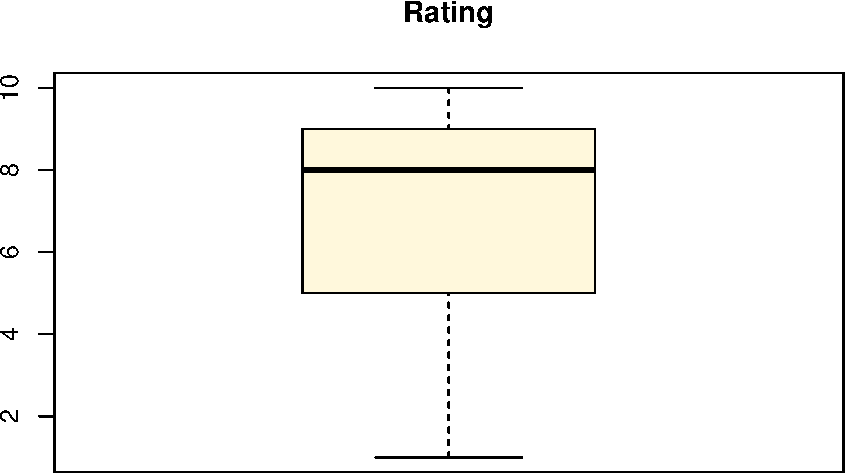
\includegraphics{practica-original_files/figure-latex/unnamed-chunk-87-1.pdf}

Como medidas de dispersión, se va a calcular la \textbf{desviación
típica}:

\begin{Shaded}
\begin{Highlighting}[]
\CommentTok{# Desviación típica}
\KeywordTok{sd}\NormalTok{(datos_train}\OperatorTok{$}\NormalTok{rating)}
\end{Highlighting}
\end{Shaded}

\begin{verbatim}
## [1] 2.937406
\end{verbatim}

Como se puede observar, la desviación típica nos da un valor de 2.93.
Esto quiere decir que los valores no están concentrados en un único
valor, sino que la mayoría se sitúan en un intervalo con distancia 3
respecto de la media.

Este valor concuerda, puesto que si observamos el histograma anterior,
vemos que la mayoría de las puntuaciones se sitúan entre 5 y 10.

Esto también nos da como \textbf{conclusión} que en general las
\textbf{opiniones} sobre los medicamentos \textbf{son buenas}, puesto
que la mayor cantidad se sitúan en el intervalo {[}5,10{]}.

\subsection{3.2. Efectividad del
medicamento}\label{efectividad-del-medicamento}

En esta sección, se va a analizar si se consideran que los medicamentos
son efectivos o no. Para ello se va a analizar el atributo
\textbf{effectivenessNumber} (que mide la efectividad del medicamento,
siendo 1 menos efectivo y 5 más efectivo).

Empezamos obteniendo las frecuencias y porcentaje total de las
anotaciones de efectividad. Para ello se va a calcular la frecuencia de
dicho atributo y su porcentaje respecto del total.

\begin{Shaded}
\begin{Highlighting}[]
\CommentTok{# Obtener frecuencias del efectivenessNumber}
\KeywordTok{table}\NormalTok{(datos_train}\OperatorTok{$}\NormalTok{effectivenessNumber)}
\end{Highlighting}
\end{Shaded}

\begin{verbatim}
## 
##    1    2    3    4    5 
##  247  186  415  926 1330
\end{verbatim}

\begin{Shaded}
\begin{Highlighting}[]
\CommentTok{# Calculamos el número de documentos}
\NormalTok{numDocuments <-}\StringTok{ }\KeywordTok{dim}\NormalTok{(datos_train)[}\DecValTok{1}\NormalTok{]}

\CommentTok{# Calculamos el porcentaje de cada valor de efectividad respecto del total}
\KeywordTok{table}\NormalTok{(datos_train}\OperatorTok{$}\NormalTok{effectivenessNumber)}\OperatorTok{/}\NormalTok{numDocuments}
\end{Highlighting}
\end{Shaded}

\begin{verbatim}
## 
##          1          2          3          4          5 
## 0.07957474 0.05992268 0.13369845 0.29832474 0.42847938
\end{verbatim}

Como podemos observar, la mayoría de los medicamentos se consideran que
son efectivos. De hecho, la mayoría de los medicamentos se consideran
altamente efectivos (con un 42\%). Podemos ahora comprobar ésto mediante
el uso de la moda.

\begin{Shaded}
\begin{Highlighting}[]
\CommentTok{# Obtenemos la moda para el efectivenessNumber}
\KeywordTok{calcularModa}\NormalTok{(datos_train}\OperatorTok{$}\NormalTok{effectivenessNumber)}
\end{Highlighting}
\end{Shaded}

\begin{verbatim}
## [1] "5"
\end{verbatim}

Como resumen en general de la efectividad, se va a calcular la media y
la mediana para obtener la tendencia central de dicha variable. La media
es la siguiente:

\begin{Shaded}
\begin{Highlighting}[]
\CommentTok{# Media}
\KeywordTok{mean}\NormalTok{(datos_train}\OperatorTok{$}\NormalTok{effectivenessNumber)}
\end{Highlighting}
\end{Shaded}

\begin{verbatim}
## [1] 3.936211
\end{verbatim}

La mediana es la siguiente:

\begin{Shaded}
\begin{Highlighting}[]
\CommentTok{# Mediana}
\KeywordTok{median}\NormalTok{(datos_train}\OperatorTok{$}\NormalTok{effectivenessNumber)}
\end{Highlighting}
\end{Shaded}

\begin{verbatim}
## [1] 4
\end{verbatim}

El valor medio obtenido es 3.93 sobre 5 y la mediana es 4. Podemos
concluir con dicha información, que en general los medicamentos son
bastantes efectivos, situándose el 50\% de dichas mediciones sobre el
valor 4.

A continuación, se va a visualizar dicha información gráficamente:

\begin{Shaded}
\begin{Highlighting}[]
\CommentTok{# Histograma sobre la efectividad de los medicamentos}
\NormalTok{efecctivenessNumberExploration <-}\StringTok{ }\NormalTok{datos_train}\OperatorTok{$}\NormalTok{effectivenessNumber}

\KeywordTok{hist}\NormalTok{(efecctivenessNumberExploration,}
     \DataTypeTok{main=}\StringTok{"Efectividad de los medicamentos"}\NormalTok{,}
     \DataTypeTok{xlab=}\StringTok{"Nivel de efectividad"}\NormalTok{,}
     \DataTypeTok{ylab=}\StringTok{"Frecuencia"}\NormalTok{,}
     \DataTypeTok{border=}\StringTok{"green"}\NormalTok{,}
     \DataTypeTok{xlim=}\KeywordTok{c}\NormalTok{(}\DecValTok{1}\NormalTok{,}\DecValTok{5}\NormalTok{),}
     \DataTypeTok{col=} \StringTok{"darkseagreen1"}\NormalTok{,}
     \DataTypeTok{breaks=}\DecValTok{5}\NormalTok{,}
     \DataTypeTok{prob=}\OtherTok{TRUE}
\NormalTok{    )}
\end{Highlighting}
\end{Shaded}

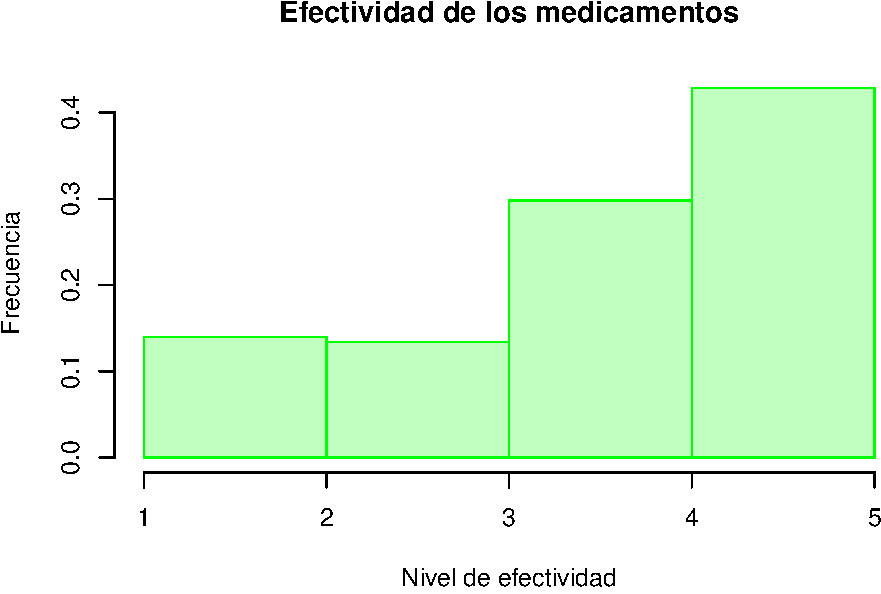
\includegraphics{practica-original_files/figure-latex/unnamed-chunk-93-1.pdf}

\begin{Shaded}
\begin{Highlighting}[]
\CommentTok{# Diagrama de densidad de la efectividad de los medicamentos}
\KeywordTok{plot}\NormalTok{(}\KeywordTok{density}\NormalTok{(datos_train}\OperatorTok{$}\NormalTok{effectivenessNumber), }
     \DataTypeTok{main=}\StringTok{"Densidad de la tasa de efectividad"}\NormalTok{,}
     \DataTypeTok{xlim=}\KeywordTok{c}\NormalTok{(}\DecValTok{0}\NormalTok{,}\DecValTok{5}\NormalTok{),}
\NormalTok{     )}
\end{Highlighting}
\end{Shaded}

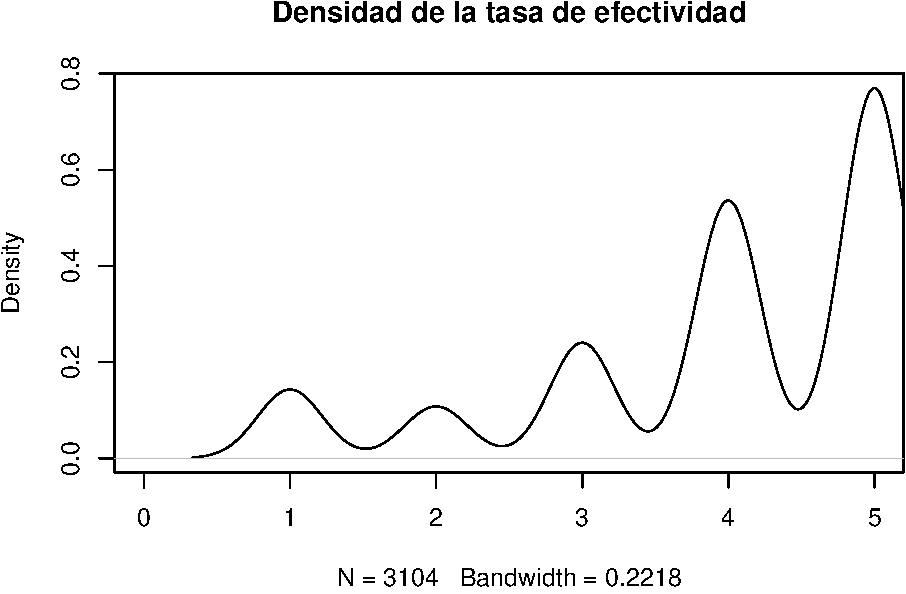
\includegraphics{practica-original_files/figure-latex/unnamed-chunk-94-1.pdf}

\begin{Shaded}
\begin{Highlighting}[]
\CommentTok{# Diagrama de sectores de la efectividad de los medicamentos}
\KeywordTok{pie}\NormalTok{(}\KeywordTok{table}\NormalTok{(datos_train}\OperatorTok{$}\NormalTok{effectivenessNumber))}
\end{Highlighting}
\end{Shaded}

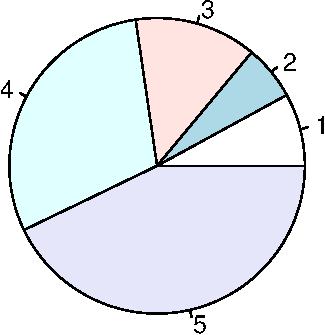
\includegraphics{practica-original_files/figure-latex/unnamed-chunk-95-1.pdf}

\begin{Shaded}
\begin{Highlighting}[]
\CommentTok{# Diagrama de cajas sobre la efectividad de los medicamentos}
\KeywordTok{boxplot}\NormalTok{(datos_train}\OperatorTok{$}\NormalTok{effectivenessNumber,}\DataTypeTok{main=}\StringTok{"Tasa de efectividad"}\NormalTok{, }\DataTypeTok{col=} \StringTok{"darkseagreen1"}\NormalTok{ )}
\end{Highlighting}
\end{Shaded}

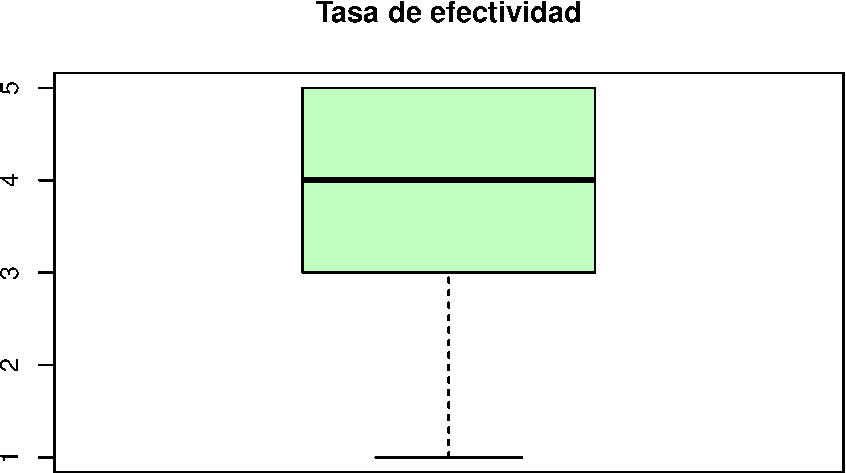
\includegraphics{practica-original_files/figure-latex/unnamed-chunk-96-1.pdf}

Como medidas de dispersión, se va a calcular la \textbf{desviación
típica}:

\begin{Shaded}
\begin{Highlighting}[]
\CommentTok{# Desviación típica}
\KeywordTok{sd}\NormalTok{(datos_train}\OperatorTok{$}\NormalTok{effectivenessNumber)}
\end{Highlighting}
\end{Shaded}

\begin{verbatim}
## [1] 1.230634
\end{verbatim}

Como se puede observar, la desviación típica nos da un valor de 1.23.
Esto quiere decir que la mayor parte de los valores se sitúan en un
intervalo con una distancia de uno de la media.

Este valor concuerda, puesto que si observamos el histograma anterior,
vemos que la mayoría de las puntuaciones se sitúan entre 3 y 5.

Esto también nos da como \textbf{conclusión} que en general los
medicamentos tienen una tasa bastante \textbf{buena de efectividad}
puesto que su tasa se sitúa entre {[}3,5{]}.

\subsection{3.3. Efectos secundarios del
medicamento}\label{efectos-secundarios-del-medicamento}

En esta sección, se va a analizar si se consideran que los medicamentos
tienen efectos secundarios o no. Para ello se va a analizar el atributo
\textbf{sideEffectsNumber} (que mide la tasa de efectos secundarios del
medicamento, siendo 1 el mínimo de efectos secundarios y 5 el máximo de
efectos secundarios).

Empezamos obteniendo las frecuencias y porcentaje total de las
anotaciones de efectos secundarios. Para ello se va a calcular la
frecuencia de dicho atributo y su porcentaje respecto del total.

\begin{Shaded}
\begin{Highlighting}[]
\CommentTok{# Obtener frecuencias del sideEffectsNumber}
\KeywordTok{table}\NormalTok{(datos_train}\OperatorTok{$}\NormalTok{sideEffectsNumber)}
\end{Highlighting}
\end{Shaded}

\begin{verbatim}
## 
##    1    2    3    4    5 
##  930 1019  612  368  175
\end{verbatim}

\begin{Shaded}
\begin{Highlighting}[]
\CommentTok{# Calculamos el número de documentos}
\NormalTok{numDocuments <-}\StringTok{ }\KeywordTok{dim}\NormalTok{(datos_train)[}\DecValTok{1}\NormalTok{]}

\CommentTok{# Calculamos el porcentaje de tasa de efectos secundarios respecto del total.}
\KeywordTok{table}\NormalTok{(datos_train}\OperatorTok{$}\NormalTok{sideEffectsNumber)}\OperatorTok{/}\NormalTok{numDocuments}
\end{Highlighting}
\end{Shaded}

\begin{verbatim}
## 
##          1          2          3          4          5 
## 0.29961340 0.32828608 0.19716495 0.11855670 0.05637887
\end{verbatim}

Como podemos observar, la mayoría de los medicamentos se consideran que
no tienen efectos secundarios severos. De hecho, la mayoría de los
medicamentos se sitúan entre sin efectos secundarios (29\%) o que tienen
efectos secundarios leves (32\%).

Podemos comprobar ésto mediante el uso de la moda.

\begin{Shaded}
\begin{Highlighting}[]
\CommentTok{# Obtenemos la moda para el sideEffectsNumber}
\KeywordTok{calcularModa}\NormalTok{(datos_train}\OperatorTok{$}\NormalTok{sideEffectsNumber)}
\end{Highlighting}
\end{Shaded}

\begin{verbatim}
## [1] "2"
\end{verbatim}

Como resumen en general, sobre la tasa de efectos secundarios, se va a
calcular la media y la mediana para calcular la tendencia central para
dicha variable. La media es la siguiente:

\begin{Shaded}
\begin{Highlighting}[]
\CommentTok{# Media}
\KeywordTok{mean}\NormalTok{(datos_train}\OperatorTok{$}\NormalTok{sideEffectsNumber)}
\end{Highlighting}
\end{Shaded}

\begin{verbatim}
## [1] 2.303802
\end{verbatim}

La mediana es la siguiente:

\begin{Shaded}
\begin{Highlighting}[]
\CommentTok{# Mediana}
\KeywordTok{median}\NormalTok{(datos_train}\OperatorTok{$}\NormalTok{sideEffectsNumber)}
\end{Highlighting}
\end{Shaded}

\begin{verbatim}
## [1] 2
\end{verbatim}

El valor medio obtenido es 2.30 sobre 5 y la mediana es 2. Podemos
concluir con dicha información, que en general los medicamentos no
tienen efectos secundarios o que dichos efectos son leves.

A continuación, se va a visualizar dicha información gráficamente:

\begin{Shaded}
\begin{Highlighting}[]
\CommentTok{# Histograma de la tasa de efectos secundarios}
\NormalTok{sideEffectsNumberExploration <-}\StringTok{ }\NormalTok{datos_train}\OperatorTok{$}\NormalTok{sideEffectsNumber}

\KeywordTok{hist}\NormalTok{(sideEffectsNumberExploration,}
     \DataTypeTok{main=}\StringTok{"Efectos secundarios de los medicamentos"}\NormalTok{,}
     \DataTypeTok{xlab=}\StringTok{"Nivel de efectos secundarios"}\NormalTok{,}
     \DataTypeTok{ylab=}\StringTok{"Frecuencia"}\NormalTok{,}
     \DataTypeTok{border=}\StringTok{"white"}\NormalTok{,}
     \DataTypeTok{xlim=}\KeywordTok{c}\NormalTok{(}\DecValTok{1}\NormalTok{,}\DecValTok{5}\NormalTok{),}
     \DataTypeTok{col=} \StringTok{"firebrick2"}\NormalTok{,}
     \DataTypeTok{breaks=}\DecValTok{5}\NormalTok{,}
     \DataTypeTok{prob=}\OtherTok{TRUE}
\NormalTok{    )}
\end{Highlighting}
\end{Shaded}

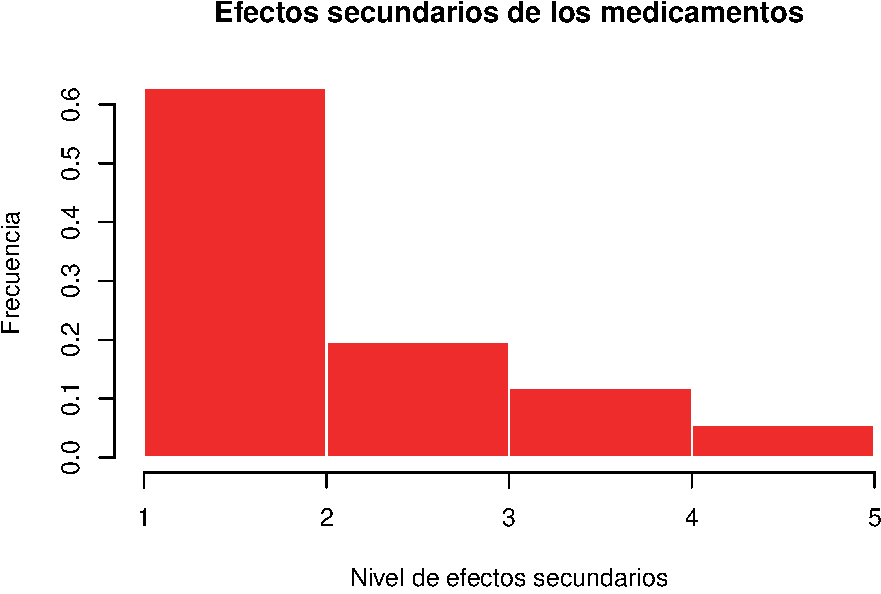
\includegraphics{practica-original_files/figure-latex/unnamed-chunk-102-1.pdf}

\begin{Shaded}
\begin{Highlighting}[]
\CommentTok{# Diagrama de densidad sobre la tasa de efectos secundarios}
\KeywordTok{plot}\NormalTok{(}\KeywordTok{density}\NormalTok{(datos_train}\OperatorTok{$}\NormalTok{sideEffectsNumber), }
     \DataTypeTok{main=}\StringTok{"Densidad de la tasa de efectos secundarios"}\NormalTok{,}
     \DataTypeTok{xlim=}\KeywordTok{c}\NormalTok{(}\DecValTok{0}\NormalTok{,}\DecValTok{5}\NormalTok{),}
\NormalTok{     )}
\end{Highlighting}
\end{Shaded}

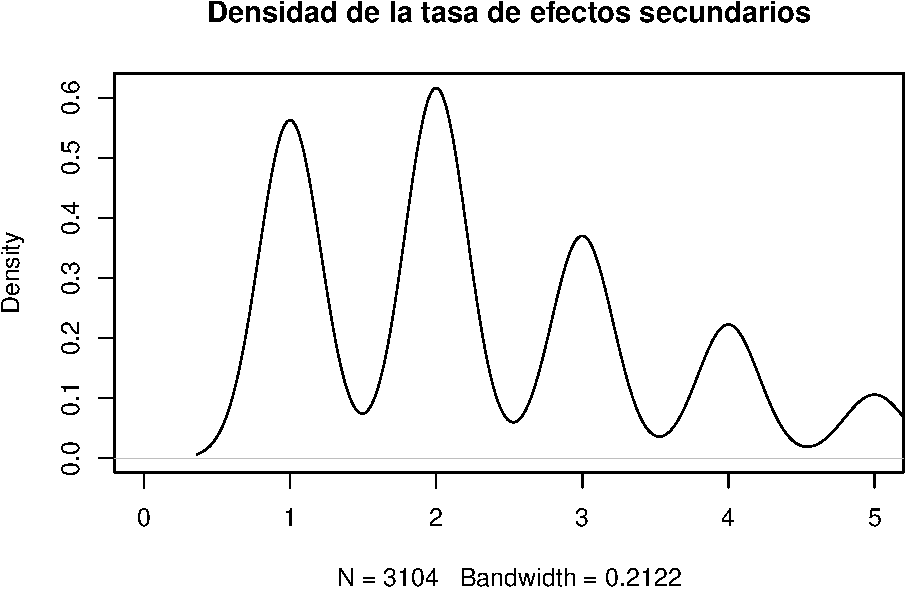
\includegraphics{practica-original_files/figure-latex/unnamed-chunk-103-1.pdf}

\begin{Shaded}
\begin{Highlighting}[]
\CommentTok{# Diagrama de sectores de los efectos secundarios de los medicamentos}
\KeywordTok{pie}\NormalTok{(}\KeywordTok{table}\NormalTok{(datos_train}\OperatorTok{$}\NormalTok{sideEffectsNumber))}
\end{Highlighting}
\end{Shaded}

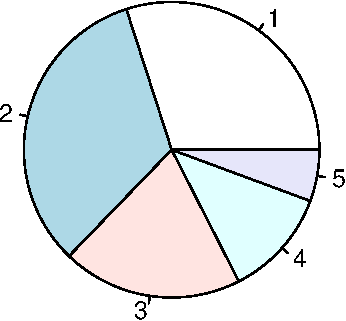
\includegraphics{practica-original_files/figure-latex/unnamed-chunk-104-1.pdf}

\begin{Shaded}
\begin{Highlighting}[]
\CommentTok{# Diagrama de cajas de los efectos secundarios de los medicamentos}
\KeywordTok{boxplot}\NormalTok{(datos_train}\OperatorTok{$}\NormalTok{effectivenessNumber,}\DataTypeTok{main=}\StringTok{"Tasa de efectos secundarios"}\NormalTok{, }\DataTypeTok{col=} \StringTok{"firebrick2"}\NormalTok{ )}
\end{Highlighting}
\end{Shaded}

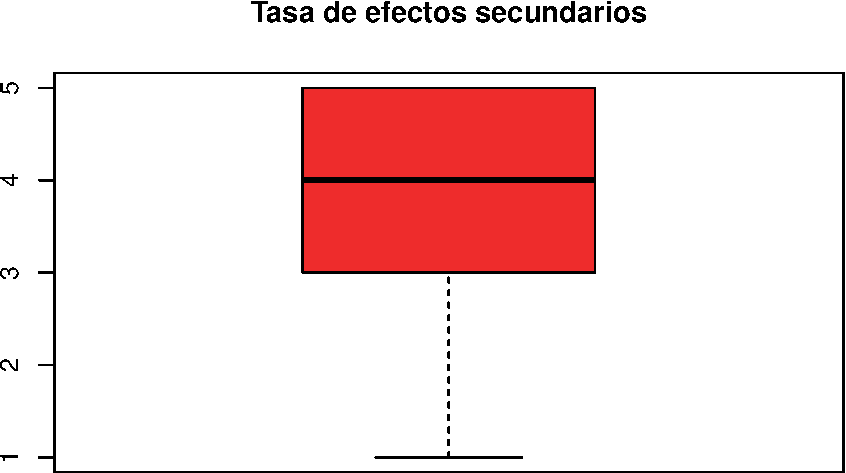
\includegraphics{practica-original_files/figure-latex/unnamed-chunk-105-1.pdf}

Como medidas de dispersión, se va a calcular la \textbf{desviación
típica}:

\begin{Shaded}
\begin{Highlighting}[]
\CommentTok{# Desviación típica}
\KeywordTok{sd}\NormalTok{(datos_train}\OperatorTok{$}\NormalTok{sideEffectsNumber)}
\end{Highlighting}
\end{Shaded}

\begin{verbatim}
## [1] 1.177525
\end{verbatim}

Como se puede observar, la desviación típica nos da un valor de 1.17.
Esto quiere decir que la mayor parte de los valores se sitúan en un
intervalo con una distancia de uno respecto la media. Este valor
concuerda, puesto que si observamos el histograma anterior, vemos que la
mayoría de las puntuaciones se sitúan entre 1 y 2.

Esto también nos da como \textbf{conclusión} que en general los
medicamentos \textbf{no tienen efectos secundarios o son muy leves}.

\subsection{3.4. Valoración ponderada sobre el
medicamento}\label{valoracion-ponderada-sobre-el-medicamento}

En esta sección, se va a analizar si se consideran que los medicamentos
son ``buenos'' o no, teniendo en cuenta la relación entre los beneficios
que aporta (efectividad) y las inconvenientes que tiene (efectos
secundarios). Para ello se va a analizar el atributo
\textbf{weightedRating} (que mide dicha relación teniendo en cuenta una
tasa de efectividad del 30\% y una tasa de efectos secundarios del
70\%), y siendo 1 peor valorado y 10 mejor valorado.

Empezamos obteniendo las frecuencias y porcentaje total de las
anotaciones sobre la puntuación ponderada. Para ello se va a calcular la
frecuencia de dicho atributo y su porcentaje respecto del total.

\begin{Shaded}
\begin{Highlighting}[]
\CommentTok{# Obtener frecuencias del weightedRating}
\KeywordTok{table}\NormalTok{(datos_train}\OperatorTok{$}\NormalTok{weightedRating)}
\end{Highlighting}
\end{Shaded}

\begin{verbatim}
## 
##    2    4    6    8   10 
##  151  236  494 1212 1011
\end{verbatim}

\begin{Shaded}
\begin{Highlighting}[]
\CommentTok{# Calculamos el número de documentos}
\NormalTok{numDocuments <-}\StringTok{ }\KeywordTok{dim}\NormalTok{(datos_train)[}\DecValTok{1}\NormalTok{]}

\CommentTok{# Calculamos el porcentaje de puntuación ponderada respecto del total.}
\KeywordTok{table}\NormalTok{(datos_train}\OperatorTok{$}\NormalTok{weightedRating)}\OperatorTok{/}\NormalTok{numDocuments}
\end{Highlighting}
\end{Shaded}

\begin{verbatim}
## 
##          2          4          6          8         10 
## 0.04864691 0.07603093 0.15914948 0.39046392 0.32570876
\end{verbatim}

Como podemos observar, la mayoría de los medicamentos se consideran que
son generalmente beneficiosos. De hecho, la mayoría de los medicamentos
se sitúan con una valoración de 8 sobre 10 teniendo en cuenta la
relación beneficio/perjuicio. Podemos comprobar ésto mediante el uso de
la moda.

\begin{Shaded}
\begin{Highlighting}[]
\CommentTok{# Obtenemos la moda para el weightedRating}
\KeywordTok{calcularModa}\NormalTok{(datos_train}\OperatorTok{$}\NormalTok{weightedRating)}
\end{Highlighting}
\end{Shaded}

\begin{verbatim}
## [1] "8"
\end{verbatim}

Como resumen en general de sobre la tasa de efectos secundarios, se va a
calcular la media y la mediana para calcular la tendencia central para
dicha variable. La media es la siguiente:

\begin{Shaded}
\begin{Highlighting}[]
\CommentTok{# Media}
\KeywordTok{mean}\NormalTok{(datos_train}\OperatorTok{$}\NormalTok{weightedRating)}
\end{Highlighting}
\end{Shaded}

\begin{verbatim}
## [1] 7.737113
\end{verbatim}

La mediana es la siguiente:

\begin{Shaded}
\begin{Highlighting}[]
\CommentTok{# Mediana}
\KeywordTok{median}\NormalTok{(datos_train}\OperatorTok{$}\NormalTok{weightedRating)}
\end{Highlighting}
\end{Shaded}

\begin{verbatim}
## [1] 8
\end{verbatim}

El valor medio obtenido es 7.52 sobre 10 y la mediana es 8. Podemos
concluir con dicha información que la puntuación general sobre los
medicamentos es de \textbf{notable}.

A continuación, se va a visualizar dicha información gráficamente:

\begin{Shaded}
\begin{Highlighting}[]
\CommentTok{# Histograma de valoración ponderada}
\NormalTok{weightedRatingExploration <-}\StringTok{ }\NormalTok{datos_train}\OperatorTok{$}\NormalTok{weightedRating}

\KeywordTok{hist}\NormalTok{(weightedRatingExploration ,}
     \DataTypeTok{main=}\StringTok{"Valoración ponderada de los medicamentos"}\NormalTok{,}
     \DataTypeTok{xlab=}\StringTok{"Rating ponderado"}\NormalTok{,}
     \DataTypeTok{ylab=}\StringTok{"Frecuencia"}\NormalTok{,}
     \DataTypeTok{border=}\StringTok{"blue"}\NormalTok{,}
     \DataTypeTok{xlim=}\KeywordTok{c}\NormalTok{(}\DecValTok{0}\NormalTok{,}\DecValTok{10}\NormalTok{),}
     \DataTypeTok{col=} \StringTok{"dodgerblue1"}\NormalTok{,}
     \DataTypeTok{breaks=}\DecValTok{5}
     
\NormalTok{    )}
\end{Highlighting}
\end{Shaded}

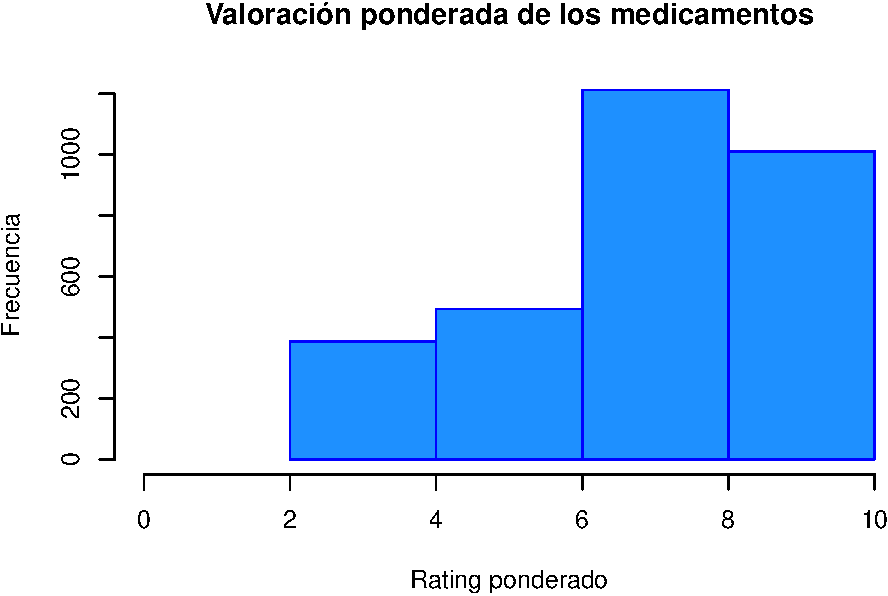
\includegraphics{practica-original_files/figure-latex/unnamed-chunk-111-1.pdf}

\begin{Shaded}
\begin{Highlighting}[]
\CommentTok{# Diagrama de densidad sobre la valoración ponderada}
\KeywordTok{plot}\NormalTok{(}\KeywordTok{density}\NormalTok{(datos_train}\OperatorTok{$}\NormalTok{weightedRating), }
     \DataTypeTok{main=}\StringTok{"Densidad de valoración ponderada"}\NormalTok{,}
     \DataTypeTok{xlim=}\KeywordTok{c}\NormalTok{(}\DecValTok{0}\NormalTok{,}\DecValTok{10}\NormalTok{),}
\NormalTok{     )}
\end{Highlighting}
\end{Shaded}

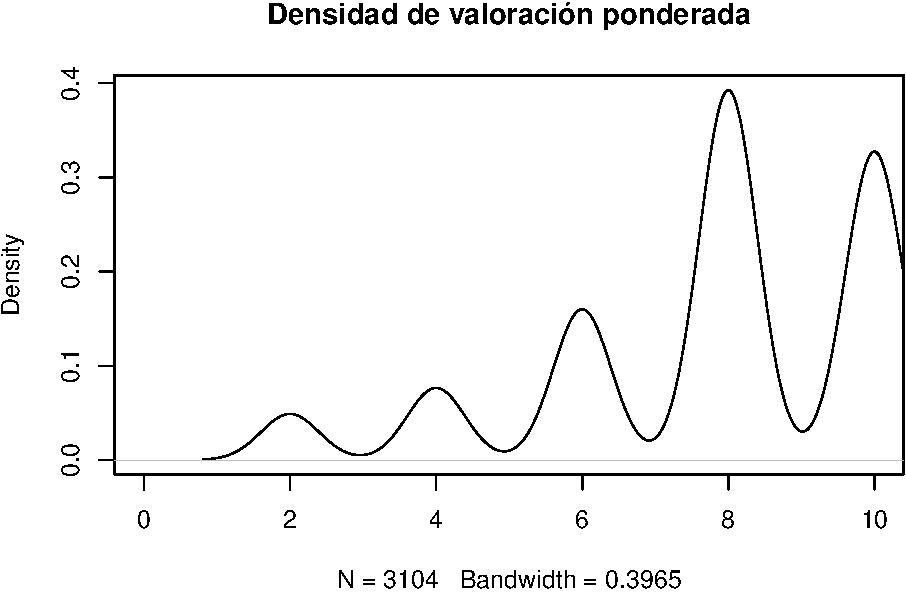
\includegraphics{practica-original_files/figure-latex/unnamed-chunk-112-1.pdf}

\begin{Shaded}
\begin{Highlighting}[]
\CommentTok{# Diagrama de sectores sobre la valoración ponderada}
\KeywordTok{pie}\NormalTok{(}\KeywordTok{table}\NormalTok{(datos_train}\OperatorTok{$}\NormalTok{weightedRating))}
\end{Highlighting}
\end{Shaded}

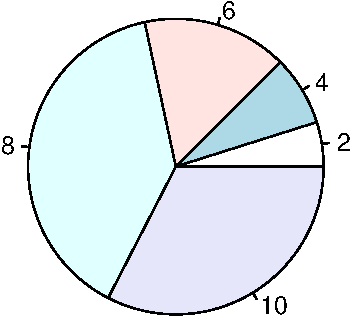
\includegraphics{practica-original_files/figure-latex/unnamed-chunk-113-1.pdf}

\begin{Shaded}
\begin{Highlighting}[]
\CommentTok{# Diagrama de cajas sobre la valoración ponderada}
\KeywordTok{boxplot}\NormalTok{(datos_train}\OperatorTok{$}\NormalTok{weightedRating,}\DataTypeTok{main=}\StringTok{"Valoración ponderada"}\NormalTok{, }\DataTypeTok{col=} \StringTok{"dodgerblue1"}\NormalTok{ )}
\end{Highlighting}
\end{Shaded}

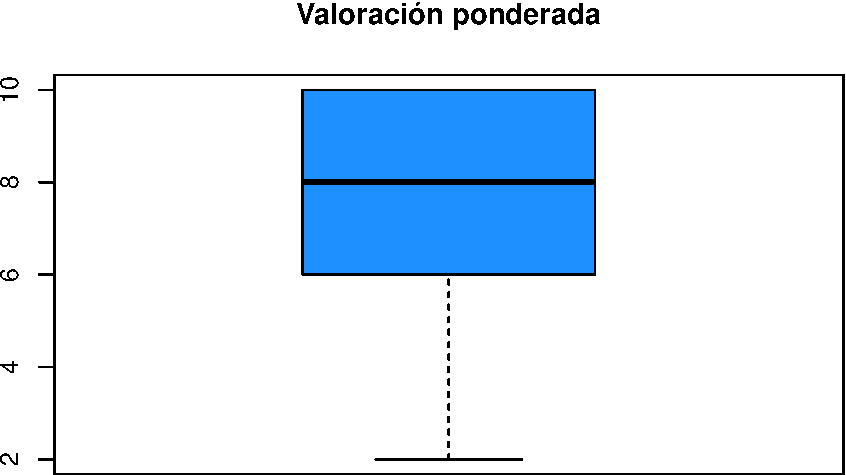
\includegraphics{practica-original_files/figure-latex/unnamed-chunk-114-1.pdf}

Como medidas de dispersión, se va a calcular la \textbf{desviación
típica}:

\begin{Shaded}
\begin{Highlighting}[]
\CommentTok{# Desviación típica}
\KeywordTok{sd}\NormalTok{(datos_train}\OperatorTok{$}\NormalTok{weightedRating)}
\end{Highlighting}
\end{Shaded}

\begin{verbatim}
## [1] 2.199924
\end{verbatim}

Como se puede observar, la desviación típica nos da un valor de 2.07.
Esto quiere decir que la mayor parte de los valores se sitúan en un
intervalo con una distancia de dos sobre la media.

Este valor concuerda, puesto que si observamos el histograma anterior,
vemos que la mayoría de las puntuaciones se sitúan entre 6 y 10.

Esto también nos da como \textbf{conclusión} que en general los
medicamentos que forman parte de este dataset \textbf{son convenientes
tomarlos}.

\subsection{3.5. Correlación sobre las
variables}\label{correlacion-sobre-las-variables}

En esta sección se va a comprobar la correlación que existe entre las
variables que miden la efectividad(effectivenessNumber), los efectos
secundarios(sideEffectsNumber), la valoración aportada por los
usuarios(rating) y la valoración ponderada que se ha realizado sobre el
medicamento(weightedRating).

Empezamos calculando la correlación entre la variable que mide la
efectividad y los efectos secundarios.

\begin{Shaded}
\begin{Highlighting}[]
\CommentTok{# Correlación lineal entre efectivenessNumber y sideEffectsNumber}
\KeywordTok{cor}\NormalTok{(datos_train[,}\KeywordTok{c}\NormalTok{(}\DecValTok{8}\NormalTok{,}\DecValTok{9}\NormalTok{)])}
\end{Highlighting}
\end{Shaded}

\begin{verbatim}
##                     sideEffectsNumber effectivenessNumber
## sideEffectsNumber           1.0000000          -0.3953789
## effectivenessNumber        -0.3953789           1.0000000
\end{verbatim}

Podemos observar que cuantos más efectos secundarios tiene, menor es la
efectividad del medicamento. Esto puede estar influido por las
valoraciones subjetivas del usuario, ya que si ha tenido una mala
experiencia (debido a los efectos secundarios) por la ingesta del
medicamento, no va a hacer énfasis en los beneficios del medicamento,
sino que hará un mayor énfasis en los aspectos negativos.

A continuación vamos a calcular la correlación entre la efectividad y la
valoración ponderada del medicamento.

\begin{Shaded}
\begin{Highlighting}[]
\CommentTok{# Correlación lineal entre efectivenessNumber y weightedRating}
\KeywordTok{cor}\NormalTok{(datos_train[,}\DecValTok{9}\OperatorTok{:}\DecValTok{10}\NormalTok{])}
\end{Highlighting}
\end{Shaded}

\begin{verbatim}
##                     effectivenessNumber weightedRating
## effectivenessNumber           1.0000000      0.9237202
## weightedRating                0.9237202      1.0000000
\end{verbatim}

Como se puede observar, cuando el medicamento es más efectivo, la
valoración ponderada del medicamento acumenta (como es obvio), y si
ahora calculamos la valoración ponderada del medicamento teniendo en
cuenta los efectos secundarios.

\begin{Shaded}
\begin{Highlighting}[]
\CommentTok{# Correlación lineal entre sideEffectsNumber y weightedRating}
\KeywordTok{cor}\NormalTok{(datos_train[,}\KeywordTok{c}\NormalTok{(}\DecValTok{8}\NormalTok{,}\DecValTok{10}\NormalTok{)])}
\end{Highlighting}
\end{Shaded}

\begin{verbatim}
##                   sideEffectsNumber weightedRating
## sideEffectsNumber          1.000000      -0.649161
## weightedRating            -0.649161       1.000000
\end{verbatim}

Observamos como si el medicamento tiene una mayor tasa de efectos
secundarios, la valoración ponderada disminuye considerablemente (obvio
porque el 70\% de la valoración ponderada tiene en cuenta los efectos
secundarios del medicamento).

Ahora vamos a comprobar la relación que existe entre la valoración dada
por el usuario y los efectos secundarios.

\begin{Shaded}
\begin{Highlighting}[]
\CommentTok{# Correlación lineal entre rating y sideEffectsNumber}
\KeywordTok{cor}\NormalTok{(datos_train[,}\KeywordTok{c}\NormalTok{(}\DecValTok{2}\NormalTok{,}\DecValTok{8}\NormalTok{)])}
\end{Highlighting}
\end{Shaded}

\begin{verbatim}
##                      rating sideEffectsNumber
## rating             1.000000         -0.682939
## sideEffectsNumber -0.682939          1.000000
\end{verbatim}

Podemos comprobar cómo si el medicamento tiene una mayor tasa de efectos
secundarios, la valoración dada por el usuario disminuye.

\begin{Shaded}
\begin{Highlighting}[]
\CommentTok{# Correlación lineal entre rating y effectivenessNumber}
\KeywordTok{cor}\NormalTok{(datos_train[,}\KeywordTok{c}\NormalTok{(}\DecValTok{2}\NormalTok{,}\DecValTok{9}\NormalTok{)])}
\end{Highlighting}
\end{Shaded}

\begin{verbatim}
##                        rating effectivenessNumber
## rating              1.0000000           0.7498171
## effectivenessNumber 0.7498171           1.0000000
\end{verbatim}

Y si la efectividad del medicamento es alta, la valoración del usuario
se incrementa.

Como observación general, se puede destacar que \textbf{la valoración
del usuario está condicionada más por la efectividad del medicamento}
(relación 1/0.74) que por los efectos secundarios (relación 1/-0.68).

Por último, vamos a observar en el siguiente gráfico cómo se relacionan
las variables entre sí en función se sus valores.

\begin{Shaded}
\begin{Highlighting}[]
\CommentTok{# Gráfico de coordenadas paralelas}
\KeywordTok{library}\NormalTok{(MASS)}
\KeywordTok{parcoord}\NormalTok{(datos_train[,}\KeywordTok{c}\NormalTok{(}\DecValTok{8}\NormalTok{,}\DecValTok{9}\NormalTok{,}\DecValTok{2}\NormalTok{,}\DecValTok{10}\NormalTok{)], }\DataTypeTok{col=}\NormalTok{datos_train}\OperatorTok{$}\NormalTok{rating,}\DataTypeTok{var.label=}\NormalTok{T)}
\end{Highlighting}
\end{Shaded}

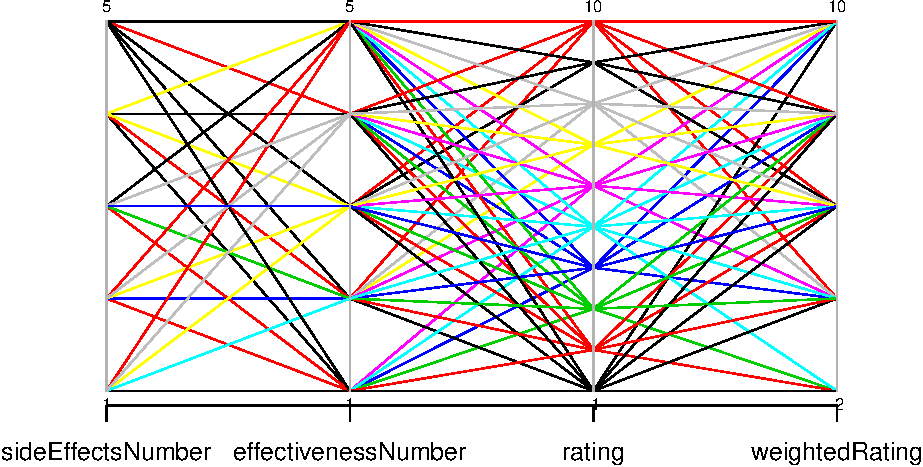
\includegraphics{practica-original_files/figure-latex/unnamed-chunk-121-1.pdf}

Por ejemplo, podemos destacar que, si el número de efectos secundarios
es 1 (no tiene efectos secundarios) y la efectividad del medicamento es
5 (muy efectivo), entonces la valoración del usuario será 10 y la
valoración ponderada será también 10.

\newpage

\section{4. Análisis de sentimientos}\label{analisis-de-sentimientos}

En este apartado vamos a realizar un análisis descriptivo de los datos.
En esta ocasión, vamos a visualizar cuáles son los sentimientos que
expresan las personas en los comentarios que escriben sobre los
distintos medicamentos que se encuentran en nuestro dataset. Lo haremos
de los comentarios relacionados con los beneficios y efectos de los
medicamentos.

La idea que se nos ocurrió consiste en saber cuáles son los medicamentos
y condiciones más frecuentes que ocurren, ya que mostrar toda la
información puede saturar la visibilidad de los datos.

\begin{Shaded}
\begin{Highlighting}[]
\KeywordTok{summary}\NormalTok{(datos_train)}

\CommentTok{#https://stackoverflow.com/questions/1686569/filter-data-frame-rows-by-a-logical-condition}
\NormalTok{condiciones =}\StringTok{ }\KeywordTok{c}\NormalTok{(}\StringTok{"depression"}\NormalTok{,}\StringTok{"acne"}\NormalTok{,}\StringTok{"anxiety"}\NormalTok{,}\StringTok{"insomnia"}\NormalTok{,}\StringTok{"birth control"}\NormalTok{,}\StringTok{"high blood pressure"}\NormalTok{)}
\NormalTok{medicamentos =}\StringTok{ }\KeywordTok{c}\NormalTok{ (}\StringTok{"lexapro"}\NormalTok{,}\StringTok{"prozac"}\NormalTok{,}\StringTok{"retin-a"}\NormalTok{,}\StringTok{"zoloft"}\NormalTok{,}\StringTok{"paxil"}\NormalTok{,}\StringTok{"propecia"}\NormalTok{)}
\end{Highlighting}
\end{Shaded}

Gracias al resumen de nuestro dataset sabemos rápidamente cuáles son las
drogas y condiciones más comunes. Ahora vamos a hacer un análisis de
sentimientos de los comentarios relacionados con estas drogas y
condiciones.

\begin{Shaded}
\begin{Highlighting}[]
\NormalTok{analisis_sentimientos <-}\StringTok{ }\ControlFlowTok{function}\NormalTok{(comentarios,titulo)\{}
  
\NormalTok{  comentarios =}\StringTok{ }\KeywordTok{Corpus}\NormalTok{(}\KeywordTok{VectorSource}\NormalTok{(comentarios))}
  
\NormalTok{  d <-}\StringTok{ }\KeywordTok{get_nrc_sentiment}\NormalTok{(comentarios}\OperatorTok{$}\NormalTok{content)}
  
  \CommentTok{#https://medium.com/swlh/exploring-sentiment-analysis-a6b53b026131}
\NormalTok{  dt <-}\StringTok{ }\KeywordTok{data.frame}\NormalTok{(}\KeywordTok{t}\NormalTok{(d))}
  
\NormalTok{  sentimientos <-}\StringTok{ }\KeywordTok{data.frame}\NormalTok{(}\KeywordTok{rowSums}\NormalTok{(dt))}
  
  \KeywordTok{names}\NormalTok{(sentimientos)[}\DecValTok{1}\NormalTok{] <-}\StringTok{ "count"}
\NormalTok{  sentimientos <-}\StringTok{ }\KeywordTok{cbind}\NormalTok{(}\StringTok{"sentiment"}\NormalTok{ =}\StringTok{ }\KeywordTok{rownames}\NormalTok{(sentimientos), sentimientos)}
  \KeywordTok{rownames}\NormalTok{(sentimientos) <-}\StringTok{ }\OtherTok{NULL}
 
  \KeywordTok{qplot}\NormalTok{(sentiment, }\DataTypeTok{data=}\NormalTok{sentimientos[}\DecValTok{1}\OperatorTok{:}\DecValTok{8}\NormalTok{,], }\DataTypeTok{weight=}\NormalTok{count, }\DataTypeTok{geom=}\StringTok{"bar"}\NormalTok{,}\DataTypeTok{fill=}\NormalTok{sentiment)}\OperatorTok{+}
\StringTok{    }\KeywordTok{ggtitle}\NormalTok{(titulo)}
  \KeywordTok{ggsave}\NormalTok{(}\KeywordTok{paste}\NormalTok{(titulo,}\StringTok{".png"}\NormalTok{),}\DataTypeTok{path =} \StringTok{'figuras/sentimientos'}\NormalTok{)}
  
  
  \KeywordTok{qplot}\NormalTok{(sentiment, }\DataTypeTok{data=}\NormalTok{sentimientos[}\DecValTok{9}\OperatorTok{:}\DecValTok{10}\NormalTok{,], }\DataTypeTok{weight=}\NormalTok{count, }\DataTypeTok{geom=}\StringTok{"bar"}\NormalTok{,}\DataTypeTok{fill=}\NormalTok{sentiment)}\OperatorTok{+}
\StringTok{    }\KeywordTok{ggtitle}\NormalTok{(titulo)}
  \KeywordTok{ggsave}\NormalTok{(}\KeywordTok{paste}\NormalTok{(titulo,}\StringTok{"_positivismo.png"}\NormalTok{),}\DataTypeTok{path =} \StringTok{'figuras/sentimientos'}\NormalTok{)}

\NormalTok{\}}
\end{Highlighting}
\end{Shaded}

Básicamente lo que llevamos a cabo en esta función es la generación del
Corpus de los comentarios pasados como parámetros (ya preprocesados). El
siguiente paso es generar la tabla de sentimientos traspuesta (sino
hacemos esto no funciona debido a la disposición de los datos). Luego
preparamos una fila en la que aparezcan el nombre de los sentimientos en
el mismo orden que la tabla y borramos los nombres de las filas. Esto
último se realiza para la correcta visualización de los datos.

Por último se lleva a cabo la representación en forma de gráficas de los
comentarios de la gente. Recordemos, están acotadas a conjuntos de
comentarios para los fármacos y condiciones más comunes, por separado.

Obtenemos las gráficas mencionadas:

\begin{Shaded}
\begin{Highlighting}[]
\ControlFlowTok{for}\NormalTok{(cadena }\ControlFlowTok{in}\NormalTok{ condiciones)\{}
\NormalTok{  datos <-}\StringTok{ }\NormalTok{datos_train[datos_train}\OperatorTok{$}\NormalTok{condition}\OperatorTok{==}\NormalTok{cadena ,]}
  \KeywordTok{analisis_sentimientos}\NormalTok{(datos}\OperatorTok{$}\NormalTok{benefits_preprocesado,}
                        \KeywordTok{paste}\NormalTok{(}\StringTok{"Comentarios_beneficios_de_condición_"}\NormalTok{,cadena))}
\NormalTok{\}}
\end{Highlighting}
\end{Shaded}

\begin{Shaded}
\begin{Highlighting}[]
\ControlFlowTok{for}\NormalTok{(cadena }\ControlFlowTok{in}\NormalTok{ condiciones)\{}
\NormalTok{  datos <-}\StringTok{ }\NormalTok{datos_train[datos_train}\OperatorTok{$}\NormalTok{condition}\OperatorTok{==}\NormalTok{cadena ,]}
  \KeywordTok{analisis_sentimientos}\NormalTok{(datos}\OperatorTok{$}\NormalTok{effects_preprocesado,}
                        \KeywordTok{paste}\NormalTok{(}\StringTok{"Comentarios_efectos_de_condición_"}\NormalTok{,cadena))}
\NormalTok{\}}
\end{Highlighting}
\end{Shaded}

\begin{Shaded}
\begin{Highlighting}[]
\ControlFlowTok{for}\NormalTok{(cadena }\ControlFlowTok{in}\NormalTok{ medicamentos)\{}
\NormalTok{  datos <-}\StringTok{ }\NormalTok{datos_train[datos_train}\OperatorTok{$}\NormalTok{urlDrugName}\OperatorTok{==}\NormalTok{cadena ,]}
  \KeywordTok{analisis_sentimientos}\NormalTok{(datos}\OperatorTok{$}\NormalTok{benefits_preprocesado,}
                        \KeywordTok{paste}\NormalTok{(}\StringTok{"Comentarios_beneficio_de_medicamento_"}\NormalTok{,cadena))}
\NormalTok{\}}
\end{Highlighting}
\end{Shaded}

\begin{Shaded}
\begin{Highlighting}[]
\ControlFlowTok{for}\NormalTok{(cadena }\ControlFlowTok{in}\NormalTok{ medicamentos)\{}
\NormalTok{  datos <-}\StringTok{ }\NormalTok{datos_train[datos_train}\OperatorTok{$}\NormalTok{urlDrugName}\OperatorTok{==}\NormalTok{cadena ,]}
  \KeywordTok{analisis_sentimientos}\NormalTok{(datos}\OperatorTok{$}\NormalTok{effects_preprocesado,}
                        \KeywordTok{paste}\NormalTok{(}\StringTok{"Comentarios_efectos_de_medicamento_"}\NormalTok{,cadena))}
\NormalTok{\}}
\end{Highlighting}
\end{Shaded}

\begin{figure}[ht]
    \centering
    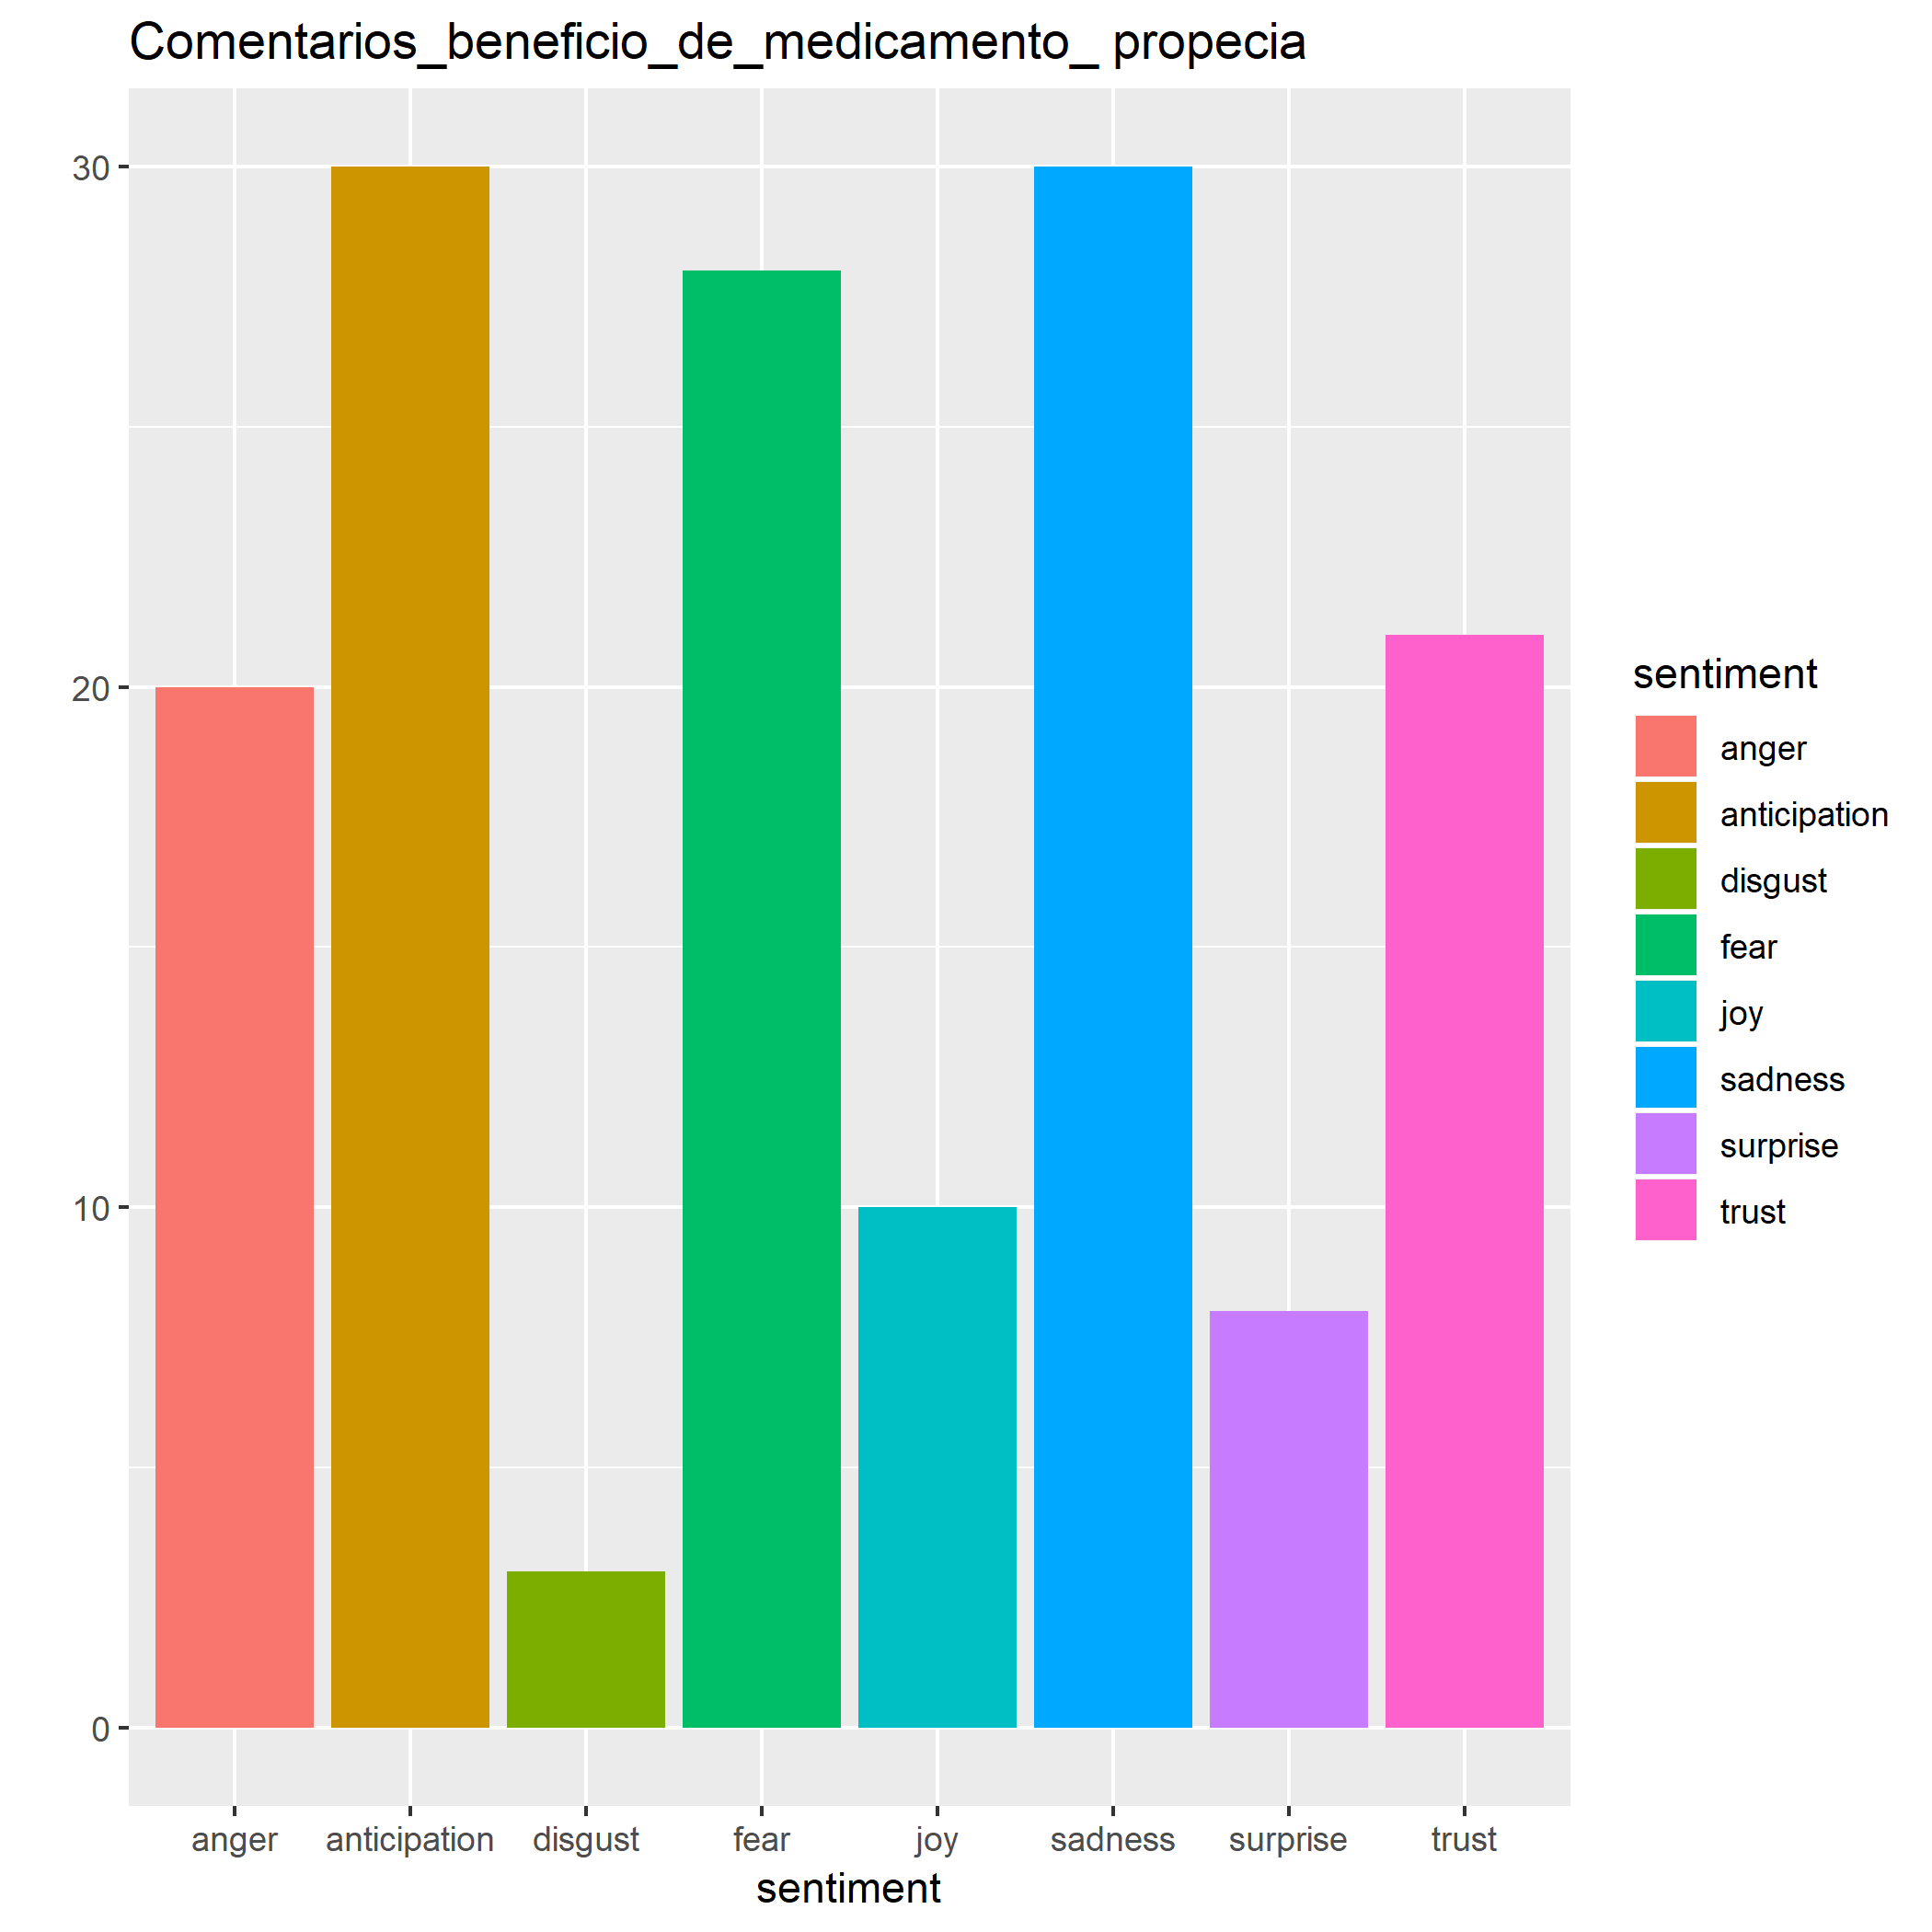
\includegraphics[width=0.5\textwidth]{figuras/elegidas/Comentarios_beneficio_de_medicamento_propecia.png}
    \caption{Análisis de sentimientos de los comentarios sobre los beneficios de los medicamentos para obtener propecia.}
    \label{fig:sentimientos:propeciaSentimiento}
\end{figure}

\begin{figure}[ht]
    \centering
    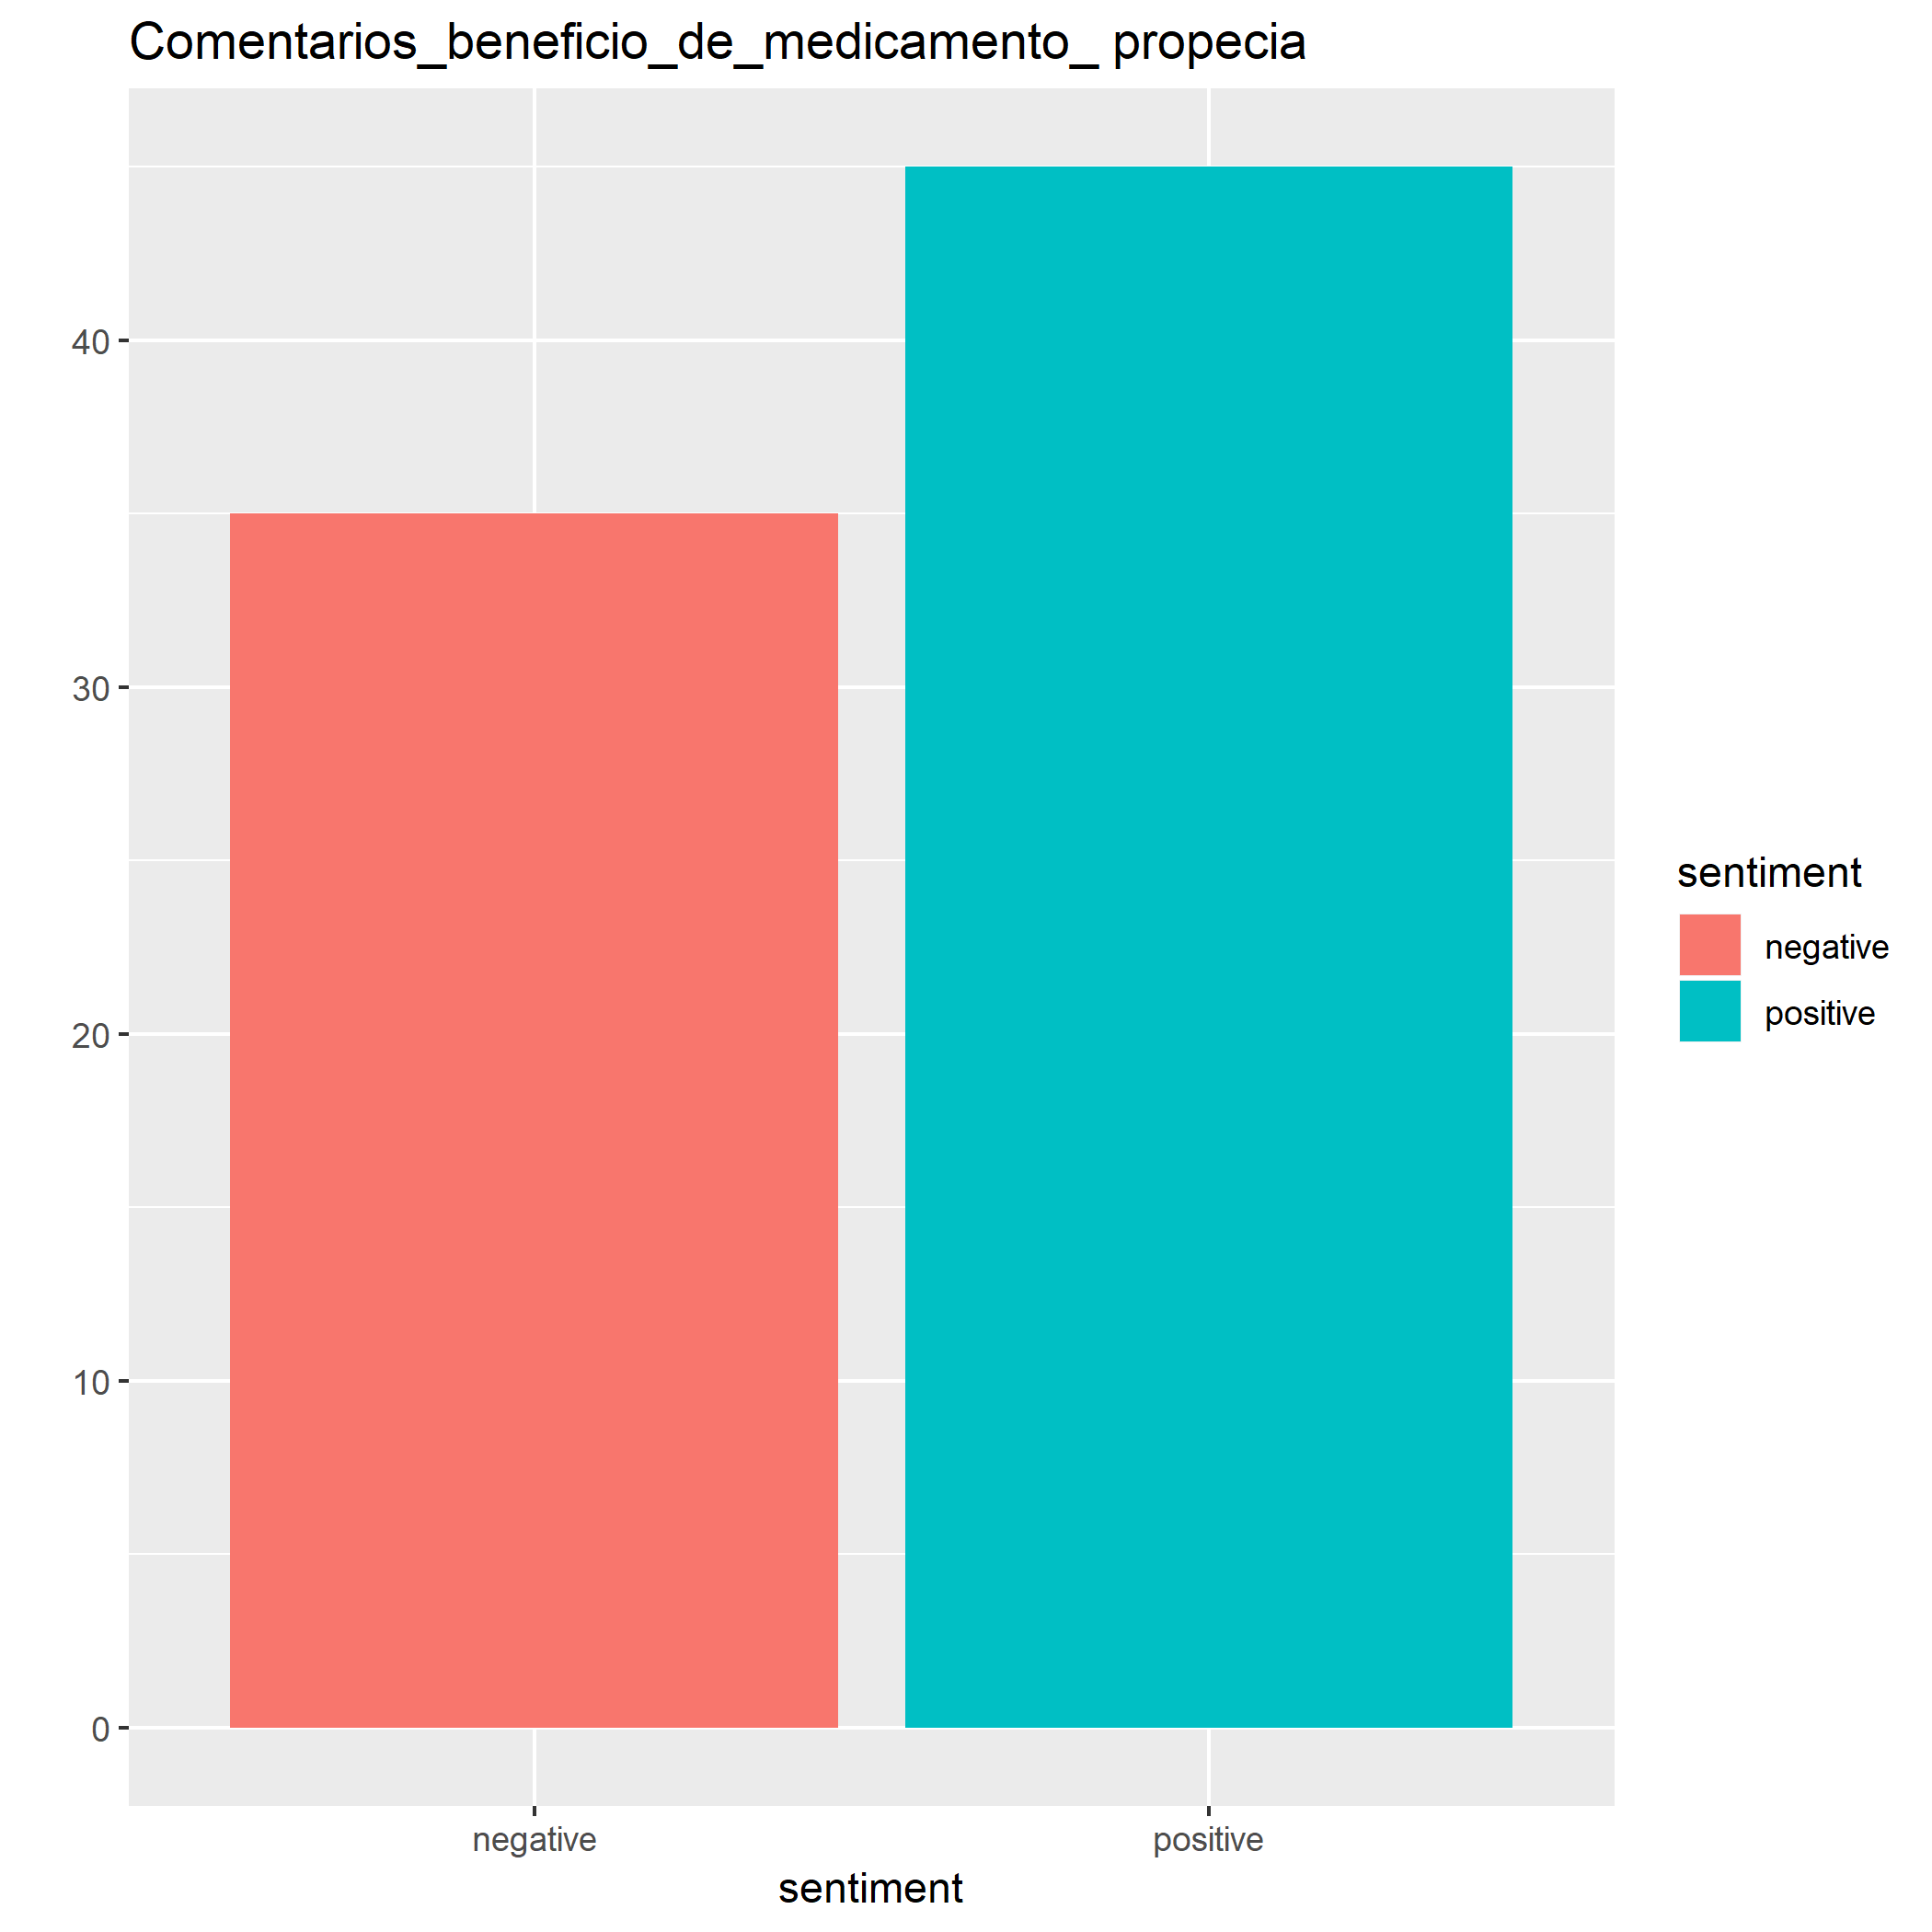
\includegraphics[width=0.5\textwidth]{figuras/elegidas/Comentarios_beneficio_de_medicamento_propecia_positivismo.png}
    \caption{Análisis de positivismo de los comentarios sobre los beneficios de los medicamentos para obtener propecia.}
    \label{fig:sentimientos:propeciaSentimiento}
\end{figure}

Hemos visualizado las imágenes resultantes y llegamos a la conclusión de
que, en general, hace una buena descripción de los datos. Por ejemplo,
para la \textbf{propecia} tenemos un altísimo contenido de sentimientos
tales como miedo, tristeza y rabia. Mientras que otros sentimientos
pasan más desapercibidos. Sin embargo, parece ser que las personas están
contentas de forma genérica para el conjunto de medicamentos que la
tratan, ya que los comentarios sobre los beneficios de los medicamentos
son más positivos que negativos. En cambio, cuando hablamos de los
efectos secundarios de este medicamento, el negativismo vence al
positivismo; se ve que los efectos secundarios que pueden acarrear este
tipo de medicinas no son muy agradables. Los sentimientos de los efectos
secundarios de los medicamentos son muy similares a los que hablan de
los beneficios, vemos que hay una concordancia de los comentarios de las
personas.

Otro dato curioso es que, de forma genérica, hay una mayor presencia de
negativismo que positivismo. Hay que darse cuenta de que las personas
están escribiendo sobre problemas de salud que tienen, por lo que el
único punto positivo que podemos extraer es cuando una persona muestra
su felicidad al ver que un cierto medicamento está surtiendo efecto (y
aún así es posible que se queje igualmente por los efectos secundarios,
por ejemplo).

Además, hay que destacar que los sentimientos están muy entremezclados
en los comentarios presentes de nuestro dataset. Los valores del rating
vendrán especificados implicitamente dependiendo del peso que le de cada
persona a esos sentimientos. En definitiva, nos damos cuenta de que
nuestro dataset es bastante subjetivo. Por ejemplo, las personas suelen
mostrarse más dispuestas a expresar comentarios para quejarse que para
informar de que un medicamento le está funcionando.

Todas estas gráficas pueden apreciarse en el anexo de esta práctica por
si se quiere ver el resto de condiciones y medicamentos analizados con
esta técnica.

Por último, mencionar que, gracias a estos resultados, hemos podido
corroborar lo expuesto tanto en el análisis exploratorio de los datos
como en el \emph{word cloud} con sentimientos que mostramos en apartados
anteriores.

\newpage

\section{5. Reglas de Asociación}\label{reglas-de-asociacion}

En esta técnica haremos un análisis descriptivo de los datos de texto ya
que, en nuestra opinión, son los que consideramos que nos pueden
permitir sacar más provecho de esta técnica.

Buscaremos la relación que existe entre las palabras expuestas en los
distintos comentarios sobre los medicamentos y tratatemos de asociarlos
a distintos conceptos para tener una mejor idea de nuestro dataset. Esto
nos permitirá saber de antemano que palabras a priori pueden tener que
ver algo con distintos efectos de los medicamentos, y también, obtener
información relevante acerca de cuestiones que se nos hayan podido
plantear (lo cual se conoce como filtraje de reglas guiado por el
usuario).

Vamos a crearnos un corpus por cada uno de los tipos de comentarios que
tenemos en cada item. Recordar que estos textos ya se encuentran
preprocesados, tal y como se puede consultar en secciones anteriores de
esta documentación.

\begin{Shaded}
\begin{Highlighting}[]
\NormalTok{benefits_corpus =}\StringTok{ }\KeywordTok{Corpus}\NormalTok{(}\KeywordTok{VectorSource}\NormalTok{(datos_train}\OperatorTok{$}\NormalTok{benefits_preprocesado))}
\NormalTok{effects_corpus =}\StringTok{ }\KeywordTok{Corpus}\NormalTok{(}\KeywordTok{VectorSource}\NormalTok{(datos_train}\OperatorTok{$}\NormalTok{effects_preprocesado))}
\end{Highlighting}
\end{Shaded}

Ahora mismo el dataset es de tipo categórico pero nosotros necesitamos
tener los datos como una cadena de caracteres para pasos posteriores.
Por tanto, todos los datos que se encuentran en estas columnas van a ser
transformados. Serán entendidos como palabras diferenciadas. Este paso
de diferenciación de las palabras de los documentos, es clave para el
funcionamiento de la técnica, puesto que nos permite obtener las
distintas palabras que posteriormente formaran los item-sets.

Una vez que obtenemos las palabras en tipo \emph{character}, algunas de
estas se quedan como palabras vacías. Debemos \emph{limpiar} estos
vacíos que se nos han generado, antes de continuar al siguiente paso.
Finalmente, una vez llevemos a cabo este último paso, ya podremos
obtener una base de datos de tipo transaccional.

\begin{Shaded}
\begin{Highlighting}[]
\NormalTok{items_benefits <-}\StringTok{ }\KeywordTok{strsplit}\NormalTok{(}\KeywordTok{as.character}\NormalTok{(benefits_corpus}\OperatorTok{$}\NormalTok{content), }\StringTok{" "}\NormalTok{)}
\NormalTok{items_effects <-}\StringTok{ }\KeywordTok{strsplit}\NormalTok{(}\KeywordTok{as.character}\NormalTok{(effects_corpus}\OperatorTok{$}\NormalTok{content), }\StringTok{" "}\NormalTok{)}

\CommentTok{# Para eliminar las cadenas vacías}
\CommentTok{# https://stackoverflow.com/questions/24178854/remove-blanks-from-strsplit-in-r}
\NormalTok{items_benefits <-}\StringTok{ }\KeywordTok{lapply}\NormalTok{(items_benefits, }\ControlFlowTok{function}\NormalTok{(x)\{x[}\OperatorTok{!}\NormalTok{x }\OperatorTok{==}\StringTok{""}\NormalTok{]\})}
\NormalTok{items_effects <-}\StringTok{ }\KeywordTok{lapply}\NormalTok{(items_effects, }\ControlFlowTok{function}\NormalTok{(x)\{x[}\OperatorTok{!}\NormalTok{x }\OperatorTok{==}\StringTok{""}\NormalTok{]\})}

\NormalTok{transactions_benefits <-}\StringTok{ }\KeywordTok{as}\NormalTok{(items_benefits,}\StringTok{"transactions"}\NormalTok{)}
\NormalTok{transactions_effects <-}\StringTok{ }\KeywordTok{as}\NormalTok{(items_effects,}\StringTok{"transactions"}\NormalTok{)}
\end{Highlighting}
\end{Shaded}

Ya tenemos los datos de textos estructurados en una base de datos
transaccional, ahora podemos aplicar la técnica para obtener las reglas
de asociación. Vamos a utilizar el algoritmo ``a priori'' visto en
clase. De lo contrario, el coste computacional y de tiempo no sería
viable para obtener este conocimineto a partir de los comentarios.

El primer parámetro que encontramos en la función se corresponde con los
datos que le proporcionamos y el segundo, un listado de parámetros
específicos. En cuanto a estos, el primero es el umbral para el soporte,
el segundo el umbral de la confianza, el tercero el target para indicar
que buscamos reglas de asociación y en el cuarto indicamos que como
mínimo empecemos con itemset de tamaño 2. De esta forma estamos
selecciondo un conjunto más reducido de reglas, que es lo que nos
interesa desde el principio para ahorrar costes de procesamiento de los
datos, al mismo tiempo que perdemos la mínima calidad posible en las
reglas.

Ordenamos por ``confidence'' a vista de mostrar posteriormente los
resultados más importantes. Entonces mostraremos las reglas que tienen
más confianza (sino no podemos realizar una buena visualización de los
datos), y finalmente visualizaremos el resultado obtenido.

\begin{Shaded}
\begin{Highlighting}[]
\NormalTok{rules_benefits <-}\StringTok{ }\KeywordTok{apriori}\NormalTok{(transactions_benefits, }\DataTypeTok{parameter =} 
                    \KeywordTok{list}\NormalTok{(}\DataTypeTok{sup =} \FloatTok{0.001}\NormalTok{, }\DataTypeTok{conf =} \FloatTok{0.7}\NormalTok{, }\DataTypeTok{target=}\StringTok{"rules"}\NormalTok{, }\DataTypeTok{minlen=}\DecValTok{2}\NormalTok{))}
\NormalTok{rules_effects <-}\StringTok{ }\KeywordTok{apriori}\NormalTok{(transactions_effects, }\DataTypeTok{parameter =}
                    \KeywordTok{list}\NormalTok{(}\DataTypeTok{sup =} \FloatTok{0.001}\NormalTok{, }\DataTypeTok{conf =} \FloatTok{0.7}\NormalTok{, }\DataTypeTok{target=}\StringTok{"rules"}\NormalTok{, }\DataTypeTok{minlen=}\DecValTok{2}\NormalTok{))}

\NormalTok{rules_benefits <-}\StringTok{ }\KeywordTok{sort}\NormalTok{(rules_benefits, }\DataTypeTok{decreasing =} \OtherTok{TRUE}\NormalTok{, }\DataTypeTok{na.last =} \OtherTok{NA}\NormalTok{,}
                       \DataTypeTok{by =} \StringTok{"confidence"}\NormalTok{)}
\NormalTok{rules_effects <-}\StringTok{ }\KeywordTok{sort}\NormalTok{(rules_effects, }\DataTypeTok{decreasing =} \OtherTok{TRUE}\NormalTok{, }\DataTypeTok{na.last =} \OtherTok{NA}\NormalTok{,}
                      \DataTypeTok{by =} \StringTok{"confidence"}\NormalTok{)}

\KeywordTok{detach}\NormalTok{(package}\OperatorTok{:}\NormalTok{tm, }\DataTypeTok{unload=}\OtherTok{TRUE}\NormalTok{) }
\KeywordTok{inspect}\NormalTok{(}\KeywordTok{head}\NormalTok{(rules_benefits,}\DecValTok{100}\NormalTok{))}
\KeywordTok{inspect}\NormalTok{(}\KeywordTok{head}\NormalTok{(rules_effects,}\DecValTok{100}\NormalTok{))}
\end{Highlighting}
\end{Shaded}

\begin{figure}[ht]
    \centering
    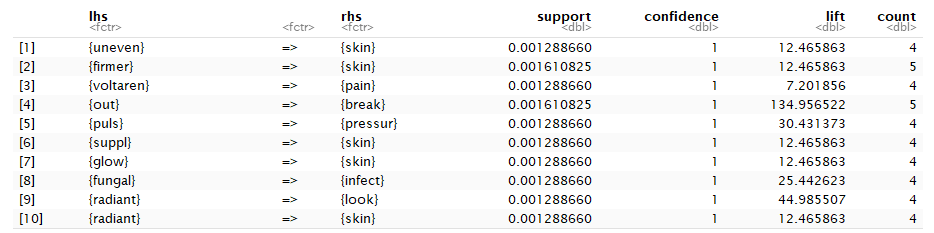
\includegraphics[width=0.7\textwidth]{figuras/asociacion/reglas_general_beneficios.png}
    \caption{inspect(head(rules\_benefits),100) para visualizar reglas más importantes de los comentarios sobre beneficios.}
    \label{fig:asociacion:reglasBenefits}
\end{figure}

\begin{figure}[ht]
    \centering
    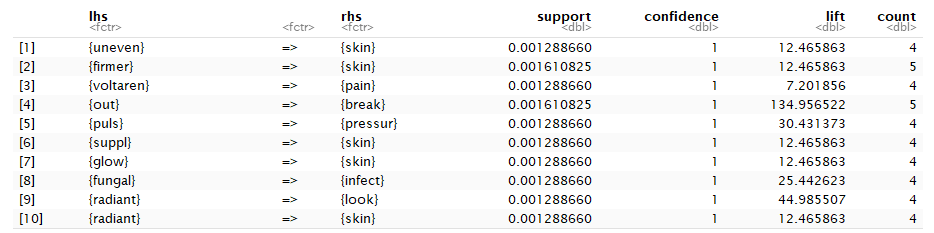
\includegraphics[width=0.7\textwidth]{figuras/asociacion/reglas_general_beneficios.png}
    \caption{inspect(head(rules\_effects),100) para visualizar reglas más importantes de los comentarios sobre efectos secundarios.}
    \label{fig:asociacion:reglasEffects}
\end{figure}

\begin{Shaded}
\begin{Highlighting}[]
\KeywordTok{plot}\NormalTok{(rules_benefits, }\DataTypeTok{method=}\StringTok{"graph"}\NormalTok{)}
\KeywordTok{title}\NormalTok{(}\StringTok{"Reglas de asociación sobre comentarios de beneficios"}\NormalTok{)}
\end{Highlighting}
\end{Shaded}

\begin{figure}[ht]
    \centering
    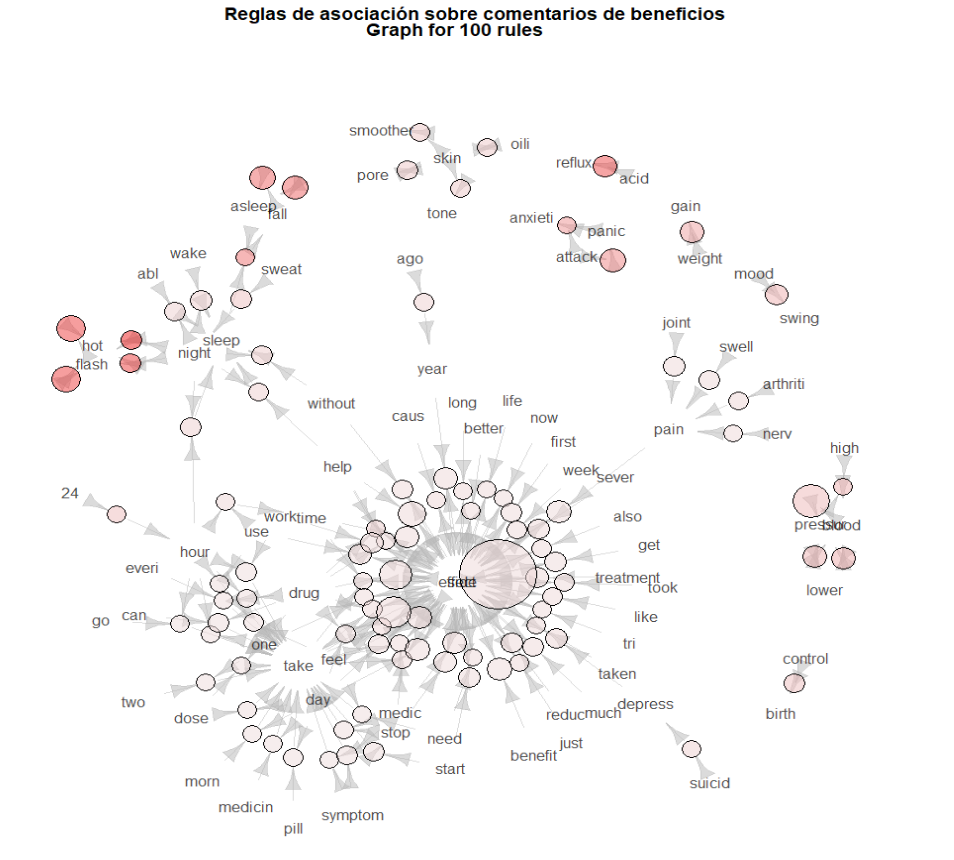
\includegraphics[width=0.7\textwidth]{figuras/asociacion/asociacion_beneficios.png}
    \caption{Mapa de reglas de asociación sobre los comentarios de beneficios.}
    \label{fig:asociacion:benefits}
\end{figure}

Al intentar pintar las reglas de asociación, nos dimos cuenta de que
plot no puede con tantas reglas al mismo tiempo, por lo que se queda con
las 100 primeras. Como las tenemos ordenadas por confianza, no nos
resulta un problema, ya que siempre que ocurra esto cogerá las 100 que
más nos interesan.

Tal y como se aprecia en el mapa de asociaciones realizado, vemos que a
simple vista las asociaciones obtenidas tienen mucho sentido. Por
ejemplo, tenemos \emph{attack} junto con \emph{panic} que están
relacionados con un lift considerable a \emph{anxieti}. Cuanto más
oscuros sean los puntos quieren decir que el lift es más alto. Por
tanto, la aparición de una de las palabras favorece la aparición de
otra.

Vemos que hay consecuentes en las reglas muy frecuentes, que ocupan el
centro o núcleo de las reglas de asociación en el mapa. Estas palabras
son principalmente \emph{effect} y \emph{side}. Esto también nos parece
prometedor, ya que tiene todo el sentido del mundo que la gente haga
comentarios siempre en torno a los efectos que tienen los medicamentos
que están probando.

Podríamos poner mil ejemplos más. La palabra \emph{acid} favorece que
aparezca la palabra \emph{reflux}. La gente cuando habla de reflujo, se
refiere al ácido del estómago que sube de forma accidental por el
esófago y causa quemazón.

En definitiva, es una buena forma de tener una vista general sobre lo
que hablan las personas en el conjunto de comentarios y tener una idea
de que conceptos utilizan más y cómo para expresar los efectos que
tienen los medicamentos.

Hicimos lo mismo para los comentarios relacionados con los efectos
secundarios.

\begin{Shaded}
\begin{Highlighting}[]
\KeywordTok{plot}\NormalTok{(rules_effects, }\DataTypeTok{method=}\StringTok{"graph"}\NormalTok{)}
\KeywordTok{title}\NormalTok{(}\StringTok{"Reglas de asociación sobre comentarios de efectos secundarios"}\NormalTok{)}
\end{Highlighting}
\end{Shaded}

\begin{figure}[ht]
    \centering
    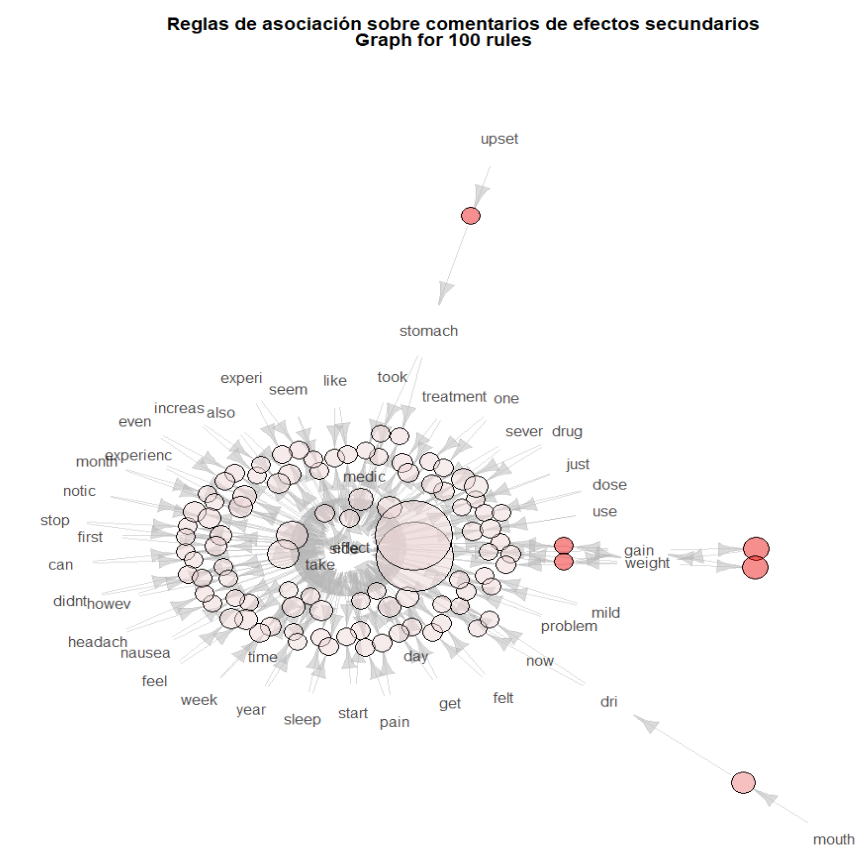
\includegraphics[width=0.6\textwidth]{figuras/asociacion/asociacion_efectos.png}
    \caption{Mapa de regla de asociación sobre los comentarios de efectos secundarios.}
    \label{fig:asociacion:effects}
\end{figure}

En este caso, vemos que no hay demasiadas asociaciones con un valor de
lift por encima significativamente del resto. Creemos que se debe a que
en este punto la gente escribe una diversidad de tipos de comentarios
mucho más grande. Es decir, quizás los comentarios sobre efectos
secundarios pueda tener una mayor cantidad de variedad sobre lo que se
habla que en los comentarios sobre los beneficios.

No obstante, volvemos a tener los mismos consecuentes más frecuentes.
Ocupando una vez más el núcleo del mapa de las reglas de asociación:
\emph{side} y \emph{effect}. Tiene sentido ya que en los efectos
secundarios vuelven a hablar de este tema de forma general, sólo que
desde un punto de vista diferente (por eso la estructura principal del
mapa y las reglas de asociación son diferentes).

Hay conceptos interesantes como \emph{nausea}, \emph{headach},
\emph{pain}\ldots{} Conceptos que están estrechamente relacionados con
efectos secundarios.

\subsection{5.1. Reglas de asociación
específicas}\label{reglas-de-asociacion-especificas}

Llegados a este punto, quisimos darle un nuevo enfoque a la extracción
de reglas de asociación a partir de estos comentarios. En los mapas
anteriores, veíamos que había demasiadas reglas enfocadas a una misma
cosa, incluso llegando a ser difícil de visualizar en algunos sitios
concretos.

Por otro lado, temíamos estar tomando solo las reglas de asociación
relacionadas con \emph{effects} y \emph{side} por ser las reglas con una
mayor confianza y despreciando otras que podían ser interesantes y que
tuvieran consecuentes en otros conceptos.

Entonces, se nos ocurrió la siguiente idea: ¿Y si enfocamos la selección
de reglas en la que el consecuente sea un término concreto que
consideremos interesante? En otras palabras, queremos realizar un
filtrado de reglas interesantes directamente guiadas por el usuario, tal
y como se ha visto en teoría.

Queremos obtener las reglas en la que los consecuentes sean los valores
de efectividad de nuestro dataset. Aquí realizamos un
``mini-preprocesamiento'', ya que está realizado en apartado anteriores,
pero en esta técnica especificamente vimos conveniente realizar estos
pequeños cambios y añadirlos en una nueva columna del dataset.

Lo primero que debíamos de hacer es tener la efectividad unida en una
sola cadena sin espacios, ya que de lo contrario no sería reconocida
como un término a la hora de generar la estructura transaccional
posterior.

\begin{Shaded}
\begin{Highlighting}[]
\NormalTok{datos_train}\OperatorTok{$}\NormalTok{effectivenessGuion[datos_train}\OperatorTok{$}\NormalTok{effectiveness }\OperatorTok{==}\StringTok{ }
\StringTok{                                 "Highly Effective"}\NormalTok{] <-}\StringTok{ "Highly-Effective"}
\NormalTok{datos_train}\OperatorTok{$}\NormalTok{effectivenessGuion[datos_train}\OperatorTok{$}\NormalTok{effectiveness }\OperatorTok{==}\StringTok{ }
\StringTok{                                 "Considerably Effective"}\NormalTok{] <-}\StringTok{ "Considerably-Effective"}
\NormalTok{datos_train}\OperatorTok{$}\NormalTok{effectivenessGuion[datos_train}\OperatorTok{$}\NormalTok{effectiveness }\OperatorTok{==}
\StringTok{                                 "Moderately Effective"}\NormalTok{] <-}\StringTok{ "Moderately-Effective"}
\NormalTok{datos_train}\OperatorTok{$}\NormalTok{effectivenessGuion[datos_train}\OperatorTok{$}\NormalTok{effectiveness }\OperatorTok{==}
\StringTok{                                 "Marginally Effective"}\NormalTok{] <-}\StringTok{ "Marginally-Effective"}
\NormalTok{datos_train}\OperatorTok{$}\NormalTok{effectivenessGuion[datos_train}\OperatorTok{$}\NormalTok{effectiveness }\OperatorTok{==}
\StringTok{                                 "Ineffective"}\NormalTok{] <-}\StringTok{ "Ineffective"}

\CommentTok{# Pasamos a factor el effectivenes unido por guiones para }
\CommentTok{# concatenarlo con los comentarios}
\NormalTok{datos_train}\OperatorTok{$}\NormalTok{effectivenessGuion =}\StringTok{ }\KeywordTok{as.factor}\NormalTok{(datos_train}\OperatorTok{$}\NormalTok{effectivenessGuion)}
\end{Highlighting}
\end{Shaded}

¿Cómo podemos hacer que estas efectividades sean cosas frecuentes en las
reglas en función de los comentarios? Tuvimos una buena idea en este
punto. Mientras discutiamos en cómo hacer que el algoritmo a priori
pudiera generar estas reglas, pensamos en coger estas etiquetas de
efectividad y ponerlas al final de cada comentario como un término más
(fila por fila). De esta forma, cada comentario tendría una palabra
final en la que aparece el nivel de efectividad que el usuario reconoce
en el medicamento y podemos pasarlo de esa forma directamente al
algoritmo.

\begin{Shaded}
\begin{Highlighting}[]
\CommentTok{# Juntamos las cadenas en una nueva columna del dataset que combina con los}
\CommentTok{# comentarios con los beneficios}
\NormalTok{datos_train}\OperatorTok{$}\NormalTok{benefits_effectiveness <-}\StringTok{ }\KeywordTok{with}\NormalTok{(datos_train, }
                    \KeywordTok{interaction}\NormalTok{(benefits_preprocesado,effectivenessGuion), }\DataTypeTok{sep=}\StringTok{" "}\NormalTok{)}
\NormalTok{datos_train}\OperatorTok{$}\NormalTok{benefits_effectiveness <-}\StringTok{ }\KeywordTok{gsub}\NormalTok{(}\StringTok{"[.]"}\NormalTok{, }\StringTok{" "}\NormalTok{, datos_train}\OperatorTok{$}\NormalTok{benefits_effectiveness)}

\CommentTok{# Hacemos lo mismo pero para los comentatios de efectos secundarios}
\NormalTok{datos_train}\OperatorTok{$}\NormalTok{effects_effectiveness <-}\StringTok{ }\KeywordTok{with}\NormalTok{(datos_train, interaction}
\NormalTok{                               (effects_preprocesado,effectivenessGuion), }\DataTypeTok{sep=}\StringTok{" "}\NormalTok{)}
\NormalTok{datos_train}\OperatorTok{$}\NormalTok{effects_effectiveness <-}\StringTok{ }\KeywordTok{gsub}\NormalTok{(}\StringTok{"[.]"}\NormalTok{, }\StringTok{" "}\NormalTok{, datos_train}\OperatorTok{$}\NormalTok{benefits_effectiveness)}

\NormalTok{datos_train}\OperatorTok{$}\NormalTok{effects_effectiveness[}\DecValTok{1}\OperatorTok{:}\DecValTok{10}\NormalTok{]}
\end{Highlighting}
\end{Shaded}

\begin{figure}[h]
    \centering
    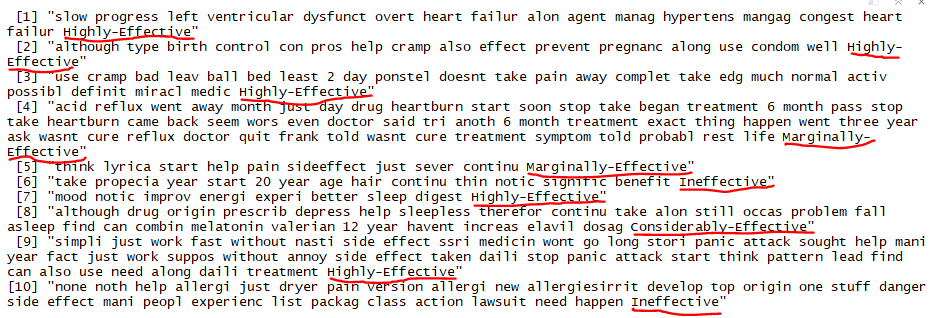
\includegraphics[width=1\textwidth]{figuras/asociacion/ejemplo_effects_effectiveness.png}
    \caption{Ilustración de preprocesamiento específico para reglas de asociación acotada a efectividad.}
    \label{fig:asociacion:preprocesamientoAsociacion}
\end{figure}

Los pasos siguientes ya son muy parecidos a los explicados
anteriormente. Generamos los corpus.

\begin{Shaded}
\begin{Highlighting}[]
\CommentTok{# Generamos los corpus con estas nuevas columnas en la que }
\CommentTok{# añadimos la efectividad como término en cada comentario}
\NormalTok{benefits_corpus =}\StringTok{ }\KeywordTok{Corpus}\NormalTok{(}\KeywordTok{VectorSource}\NormalTok{(datos_train}\OperatorTok{$}\NormalTok{benefits_effectiveness))}
\NormalTok{effects_corpus =}\StringTok{ }\KeywordTok{Corpus}\NormalTok{(}\KeywordTok{VectorSource}\NormalTok{(datos_train}\OperatorTok{$}\NormalTok{effects_effectiveness))}
\end{Highlighting}
\end{Shaded}

Separamos los términos y eliminamos términos vacíos.

\begin{Shaded}
\begin{Highlighting}[]
\CommentTok{#Separamos todas las palabras entre sí}
\NormalTok{benefits_items <-}\StringTok{ }\KeywordTok{strsplit}\NormalTok{(}\KeywordTok{as.character}\NormalTok{(benefits_corpus}\OperatorTok{$}\NormalTok{content), }\StringTok{" "}\NormalTok{)}
\NormalTok{effects_items <-}\StringTok{ }\KeywordTok{strsplit}\NormalTok{(}\KeywordTok{as.character}\NormalTok{(effects_corpus}\OperatorTok{$}\NormalTok{content), }\StringTok{" "}\NormalTok{)}
\CommentTok{# Para eliminar las cadenas vacías}
\CommentTok{# https://stackoverflow.com/questions/24178854/remove-blanks-from-strsplit-in-r}
\NormalTok{benefits_items <-}\StringTok{ }\KeywordTok{lapply}\NormalTok{(benefits_items, }\ControlFlowTok{function}\NormalTok{(x)\{x[}\OperatorTok{!}\NormalTok{x }\OperatorTok{==}\StringTok{""}\NormalTok{]\})}
\NormalTok{effects_items <-}\StringTok{ }\KeywordTok{lapply}\NormalTok{(effects_items, }\ControlFlowTok{function}\NormalTok{(x)\{x[}\OperatorTok{!}\NormalTok{x }\OperatorTok{==}\StringTok{""}\NormalTok{]\})}
\end{Highlighting}
\end{Shaded}

Generamos las estructuras transaccionales.

\begin{Shaded}
\begin{Highlighting}[]
\CommentTok{#Generamos la estructura de datos transaccional}
\NormalTok{benefits_transactions <-}\StringTok{ }\KeywordTok{as}\NormalTok{(benefits_items,}\StringTok{"transactions"}\NormalTok{)}
\NormalTok{effects_transactions <-}\StringTok{ }\KeywordTok{as}\NormalTok{(effects_items,}\StringTok{"transactions"}\NormalTok{)}
\end{Highlighting}
\end{Shaded}

Ahora tenemos que aplicar el algoritmo a priori. La estrategia consiste
en hacer que los consecuentes frecuentes sean los tipos de efectividad
que puede tener los medicamentos; es una forma más de filtrar reglas y
no quedarnos con todas (ya que hemos visto en teoría que esto es
computacionalmente muy costoso). Por ello, especificamos que los
consecuentes de las reglas obtenidas sean cada una de las etiquetas
posibles de este campo (con el guión puesto para las palabras compuestas
como hicimos anteriormente). Los parámetros han sido fijados para que
nos devuelva un conjunto de reglas razonable.

Finalmente, ordenamos las reglas obtenidas por la confianza que tienen
de mayor a menor.

\begin{Shaded}
\begin{Highlighting}[]
\NormalTok{benefits_rulesInnefective <-}\StringTok{ }\KeywordTok{apriori}\NormalTok{ (}\DataTypeTok{data=}\NormalTok{benefits_transactions, }
                             \DataTypeTok{parameter=}\KeywordTok{list}\NormalTok{ (}\DataTypeTok{supp=}\FloatTok{0.0007}\NormalTok{,}\DataTypeTok{conf =} \FloatTok{0.9}\NormalTok{, }\DataTypeTok{minlen=}\DecValTok{2}\NormalTok{), }
                             \DataTypeTok{appearance =} \KeywordTok{list}\NormalTok{(}\DataTypeTok{default=}\StringTok{"lhs"}\NormalTok{,}\DataTypeTok{rhs=}\KeywordTok{c}\NormalTok{(}\StringTok{"Ineffective"}\NormalTok{)), }
                             \DataTypeTok{control =} \KeywordTok{list}\NormalTok{ (}\DataTypeTok{verbose=}\NormalTok{F))}

\NormalTok{benefits_rulesHighlyEffective <-}\StringTok{ }\KeywordTok{apriori}\NormalTok{ (}\DataTypeTok{data=}\NormalTok{benefits_transactions, }
                             \DataTypeTok{parameter=}\KeywordTok{list}\NormalTok{ (}\DataTypeTok{supp=}\FloatTok{0.0007}\NormalTok{,}\DataTypeTok{conf =} \FloatTok{0.9}\NormalTok{, }\DataTypeTok{minlen=}\DecValTok{2}\NormalTok{), }
                             \DataTypeTok{appearance =} \KeywordTok{list}\NormalTok{(}\DataTypeTok{default=}\StringTok{"lhs"}\NormalTok{,}
                                               \DataTypeTok{rhs=}\KeywordTok{c}\NormalTok{(}\StringTok{"Highly-Effective"}\NormalTok{)), }
                             \DataTypeTok{control =} \KeywordTok{list}\NormalTok{ (}\DataTypeTok{verbose=}\NormalTok{F))}

\NormalTok{benefits_rulesConsiderablyEffective <-}\StringTok{ }\KeywordTok{apriori}\NormalTok{ (}\DataTypeTok{data=}\NormalTok{benefits_transactions, }
                              \DataTypeTok{parameter=}\KeywordTok{list}\NormalTok{ (}\DataTypeTok{supp=}\FloatTok{0.0007}\NormalTok{,}\DataTypeTok{conf =} \FloatTok{0.9}\NormalTok{, }\DataTypeTok{minlen=}\DecValTok{2}\NormalTok{), }
                              \DataTypeTok{appearance =} \KeywordTok{list}\NormalTok{(}\DataTypeTok{default=}\StringTok{"lhs"}\NormalTok{,}
                                                \DataTypeTok{rhs=}\KeywordTok{c}\NormalTok{(}\StringTok{"Considerably-Effective"}\NormalTok{)), }
                              \DataTypeTok{control =} \KeywordTok{list}\NormalTok{ (}\DataTypeTok{verbose=}\NormalTok{F))}

\NormalTok{benefits_rulesModeratelyEffective <-}\StringTok{ }\KeywordTok{apriori}\NormalTok{ (}\DataTypeTok{data=}\NormalTok{benefits_transactions, }
                              \DataTypeTok{parameter=}\KeywordTok{list}\NormalTok{ (}\DataTypeTok{supp=}\FloatTok{0.0007}\NormalTok{,}\DataTypeTok{conf =} \FloatTok{0.9}\NormalTok{, }\DataTypeTok{minlen=}\DecValTok{2}\NormalTok{), }
                              \DataTypeTok{appearance =} \KeywordTok{list}\NormalTok{(}\DataTypeTok{default=}\StringTok{"lhs"}\NormalTok{,}
                                                \DataTypeTok{rhs=}\KeywordTok{c}\NormalTok{(}\StringTok{"Moderately-Effective"}\NormalTok{)), }
                              \DataTypeTok{control =} \KeywordTok{list}\NormalTok{ (}\DataTypeTok{verbose=}\NormalTok{F))}

\NormalTok{benefits_rulesMarginallyEffective <-}\StringTok{ }\KeywordTok{apriori}\NormalTok{ (}\DataTypeTok{data=}\NormalTok{benefits_transactions, }
                             \DataTypeTok{parameter=}\KeywordTok{list}\NormalTok{ (}\DataTypeTok{supp=}\FloatTok{0.0007}\NormalTok{,}\DataTypeTok{conf =} \FloatTok{0.9}\NormalTok{, }\DataTypeTok{minlen=}\DecValTok{2}\NormalTok{), }
                             \DataTypeTok{appearance =} \KeywordTok{list}\NormalTok{(}\DataTypeTok{default=}\StringTok{"lhs"}\NormalTok{,}
                                               \DataTypeTok{rhs=}\KeywordTok{c}\NormalTok{(}\StringTok{"Marginally-Effective"}\NormalTok{)), }
                             \DataTypeTok{control =} \KeywordTok{list}\NormalTok{ (}\DataTypeTok{verbose=}\NormalTok{F))}

\NormalTok{benefits_rulesInnefective <-}\StringTok{ }
\StringTok{  }\KeywordTok{sort}\NormalTok{(benefits_rulesInnefective, }\DataTypeTok{decreasing=}\OtherTok{TRUE}\NormalTok{, }\DataTypeTok{na.last=}\OtherTok{NA}\NormalTok{, }\DataTypeTok{by=}\StringTok{"confidence"}\NormalTok{)}
\NormalTok{benefits_rulesHighlyEffective <-}\StringTok{ }
\StringTok{  }\KeywordTok{sort}\NormalTok{(benefits_rulesHighlyEffective, }\DataTypeTok{decreasing=}\OtherTok{TRUE}\NormalTok{, }\DataTypeTok{na.last =} \OtherTok{NA}\NormalTok{, }\DataTypeTok{by=}\StringTok{"confidence"}\NormalTok{)}
\NormalTok{benefits_rulesConsiderablyEffective <-}\StringTok{ }
\StringTok{  }\KeywordTok{sort}\NormalTok{(benefits_rulesConsiderablyEffective, }\DataTypeTok{decreasing=}\OtherTok{TRUE}\NormalTok{, }\DataTypeTok{na.last=}\OtherTok{NA}\NormalTok{, }\DataTypeTok{by=}\StringTok{"confidence"}\NormalTok{)}
\NormalTok{benefits_rulesModeratelyEffective <-}\StringTok{ }
\StringTok{  }\KeywordTok{sort}\NormalTok{(benefits_rulesModeratelyEffective, }\DataTypeTok{decreasing=}\OtherTok{TRUE}\NormalTok{, }\DataTypeTok{na.last=}\OtherTok{NA}\NormalTok{, }\DataTypeTok{by=}\StringTok{"confidence"}\NormalTok{)}
\NormalTok{benefits_rulesMarginallyEffective <-}\StringTok{ }
\StringTok{  }\KeywordTok{sort}\NormalTok{(benefits_rulesMarginallyEffective, }\DataTypeTok{decreasing=}\OtherTok{TRUE}\NormalTok{, }\DataTypeTok{na.last=}\OtherTok{NA}\NormalTok{, }\DataTypeTok{by=}\StringTok{"confidence"}\NormalTok{)}
\end{Highlighting}
\end{Shaded}

Podemos mostrar las 10 reglas de mayor confianza relacionadas con cada
uno de los consecuentes.

\begin{Shaded}
\begin{Highlighting}[]
\KeywordTok{detach}\NormalTok{(package}\OperatorTok{:}\NormalTok{tm, }\DataTypeTok{unload=}\OtherTok{TRUE}\NormalTok{)}
\KeywordTok{inspect}\NormalTok{(}\KeywordTok{head}\NormalTok{(benefits_rulesInnefective,}\DecValTok{10}\NormalTok{))}
\KeywordTok{inspect}\NormalTok{(}\KeywordTok{head}\NormalTok{(benefits_rulesHighlyEffective,}\DecValTok{10}\NormalTok{))}
\KeywordTok{inspect}\NormalTok{(}\KeywordTok{head}\NormalTok{(benefits_rulesConsiderablyEffective,}\DecValTok{10}\NormalTok{))}
\KeywordTok{inspect}\NormalTok{(}\KeywordTok{head}\NormalTok{(benefits_rulesModeratelyEffective,}\DecValTok{10}\NormalTok{))}
\KeywordTok{inspect}\NormalTok{(}\KeywordTok{head}\NormalTok{(benefits_rulesMarginallyEffective,}\DecValTok{10}\NormalTok{))}
\KeywordTok{library}\NormalTok{(tm)}
\end{Highlighting}
\end{Shaded}

Hacemos el mismo proceso pero con los comentatios de los efectos
secundarios.

\begin{Shaded}
\begin{Highlighting}[]
\NormalTok{effects_rulesInnefective <-}\StringTok{ }\KeywordTok{apriori}\NormalTok{ (}\DataTypeTok{data=}\NormalTok{effects_transactions, }
                                 \DataTypeTok{parameter=}\KeywordTok{list}\NormalTok{ (}\DataTypeTok{supp=}\FloatTok{0.0007}\NormalTok{,}\DataTypeTok{conf =} \FloatTok{0.9}\NormalTok{, }\DataTypeTok{minlen=}\DecValTok{2}\NormalTok{), }
                                 \DataTypeTok{appearance =} \KeywordTok{list}\NormalTok{(}\DataTypeTok{default=}\StringTok{"lhs"}\NormalTok{,}\DataTypeTok{rhs=}\KeywordTok{c}\NormalTok{(}\StringTok{"Ineffective"}\NormalTok{)), }
                                 \DataTypeTok{control =} \KeywordTok{list}\NormalTok{ (}\DataTypeTok{verbose=}\NormalTok{F))}

\NormalTok{effects_rulesHighlyEffective <-}\StringTok{ }\KeywordTok{apriori}\NormalTok{ (}\DataTypeTok{data=}\NormalTok{effects_transactions, }
                             \DataTypeTok{parameter=}\KeywordTok{list}\NormalTok{ (}\DataTypeTok{supp=}\FloatTok{0.0007}\NormalTok{,}\DataTypeTok{conf =} \FloatTok{0.9}\NormalTok{, }\DataTypeTok{minlen=}\DecValTok{2}\NormalTok{), }
                             \DataTypeTok{appearance =} \KeywordTok{list}\NormalTok{(}\DataTypeTok{default=}\StringTok{"lhs"}\NormalTok{,}\DataTypeTok{rhs=}\KeywordTok{c}\NormalTok{(}\StringTok{"Highly-Effective"}\NormalTok{)), }
                             \DataTypeTok{control =} \KeywordTok{list}\NormalTok{ (}\DataTypeTok{verbose=}\NormalTok{F))}

\NormalTok{effects_rulesConsiderablyEffective <-}\StringTok{ }\KeywordTok{apriori}\NormalTok{ (}\DataTypeTok{data=}\NormalTok{effects_transactions, }
                                \DataTypeTok{parameter=}\KeywordTok{list}\NormalTok{ (}\DataTypeTok{supp=}\FloatTok{0.0007}\NormalTok{,}\DataTypeTok{conf =} \FloatTok{0.9}\NormalTok{, }\DataTypeTok{minlen=}\DecValTok{2}\NormalTok{), }
                                \DataTypeTok{appearance =} \KeywordTok{list}\NormalTok{(}\DataTypeTok{default=}\StringTok{"lhs"}\NormalTok{,}
                                                  \DataTypeTok{rhs=}\KeywordTok{c}\NormalTok{(}\StringTok{"Considerably-Effective"}\NormalTok{)), }
                                \DataTypeTok{control =} \KeywordTok{list}\NormalTok{ (}\DataTypeTok{verbose=}\NormalTok{F))}

\NormalTok{effects_rulesModeratelyEffective <-}\StringTok{ }\KeywordTok{apriori}\NormalTok{ (}\DataTypeTok{data=}\NormalTok{effects_transactions, }
                                \DataTypeTok{parameter=}\KeywordTok{list}\NormalTok{ (}\DataTypeTok{supp=}\FloatTok{0.0007}\NormalTok{,}\DataTypeTok{conf =} \FloatTok{0.9}\NormalTok{, }\DataTypeTok{minlen=}\DecValTok{2}\NormalTok{), }
                                \DataTypeTok{appearance =} \KeywordTok{list}\NormalTok{(}\DataTypeTok{default=}\StringTok{"lhs"}\NormalTok{,}
                                                  \DataTypeTok{rhs=}\KeywordTok{c}\NormalTok{(}\StringTok{"Moderately-Effective"}\NormalTok{)), }
                                \DataTypeTok{control =} \KeywordTok{list}\NormalTok{ (}\DataTypeTok{verbose=}\NormalTok{F))}

\NormalTok{effects_rulesMarginallyEffective <-}\StringTok{ }\KeywordTok{apriori}\NormalTok{ (}\DataTypeTok{data=}\NormalTok{effects_transactions, }
                                     \DataTypeTok{parameter=}\KeywordTok{list}\NormalTok{ (}\DataTypeTok{supp=}\FloatTok{0.0007}\NormalTok{,}\DataTypeTok{conf =} \FloatTok{0.9}\NormalTok{, }\DataTypeTok{minlen=}\DecValTok{2}\NormalTok{), }
                                     \DataTypeTok{appearance =} \KeywordTok{list}\NormalTok{(}\DataTypeTok{default=}\StringTok{"lhs"}\NormalTok{,}
                                                       \DataTypeTok{rhs=}\KeywordTok{c}\NormalTok{(}\StringTok{"Marginally-Effective"}\NormalTok{)), }
                                     \DataTypeTok{control =} \KeywordTok{list}\NormalTok{ (}\DataTypeTok{verbose=}\NormalTok{F))}


\NormalTok{effects_rulesInnefective <-}\StringTok{ }\KeywordTok{sort}\NormalTok{(effects_rulesInnefective, }
                                 \DataTypeTok{decreasing=}\OtherTok{TRUE}\NormalTok{, }\DataTypeTok{na.last=}\OtherTok{NA}\NormalTok{, }\DataTypeTok{by=}\StringTok{"confidence"}\NormalTok{)}
\NormalTok{effects_rulesHighlyEffective <-}\StringTok{ }\KeywordTok{sort}\NormalTok{(effects_rulesHighlyEffective, }
                                     \DataTypeTok{decreasing=}\OtherTok{TRUE}\NormalTok{, }\DataTypeTok{na.last=}\OtherTok{NA}\NormalTok{, }\DataTypeTok{by=}\StringTok{"confidence"}\NormalTok{)}
\NormalTok{effects_rulesConsiderablyEffective <-}\StringTok{ }\KeywordTok{sort}\NormalTok{(effects_rulesConsiderablyEffective, }
                                           \DataTypeTok{decreasing=}\OtherTok{TRUE}\NormalTok{, }\DataTypeTok{na.last =} \OtherTok{NA}\NormalTok{, }\DataTypeTok{by=}\StringTok{"confidence"}\NormalTok{)}
\NormalTok{effects_rulesModeratelyEffective <-}\StringTok{ }\KeywordTok{sort}\NormalTok{(effects_rulesModeratelyEffective, }
                                         \DataTypeTok{decreasing=}\OtherTok{TRUE}\NormalTok{, }\DataTypeTok{na.last =} \OtherTok{NA}\NormalTok{, }\DataTypeTok{by=}\StringTok{"confidence"}\NormalTok{)}
\NormalTok{effects_rulesMarginallyEffective <-}\StringTok{ }\KeywordTok{sort}\NormalTok{(effects_rulesMarginallyEffective,}
                                         \DataTypeTok{decreasing=}\OtherTok{TRUE}\NormalTok{, }\DataTypeTok{na.last=}\OtherTok{NA}\NormalTok{, }\DataTypeTok{by=}\StringTok{"confidence"}\NormalTok{)}
\end{Highlighting}
\end{Shaded}

Podríamos mostrar las 10 reglas con mayor confianza relacionadas con
cada uno de los consecuentes si lo deseamos.

\begin{Shaded}
\begin{Highlighting}[]
\KeywordTok{detach}\NormalTok{(package}\OperatorTok{:}\NormalTok{tm, }\DataTypeTok{unload=}\OtherTok{TRUE}\NormalTok{)}
\KeywordTok{inspect}\NormalTok{(}\KeywordTok{head}\NormalTok{(effects_rulesInnefective,}\DecValTok{10}\NormalTok{))}
\KeywordTok{inspect}\NormalTok{(}\KeywordTok{head}\NormalTok{(effects_rulesHighlyEffective,}\DecValTok{10}\NormalTok{))}
\KeywordTok{inspect}\NormalTok{(}\KeywordTok{head}\NormalTok{(effects_rulesConsiderablyEffective,}\DecValTok{10}\NormalTok{))}
\KeywordTok{inspect}\NormalTok{(}\KeywordTok{head}\NormalTok{(effects_rulesModeratelyEffective,}\DecValTok{10}\NormalTok{))}
\KeywordTok{inspect}\NormalTok{(}\KeywordTok{head}\NormalTok{(effects_rulesMarginallyEffective,}\DecValTok{10}\NormalTok{))}
\KeywordTok{library}\NormalTok{(tm)}
\end{Highlighting}
\end{Shaded}

Finalmente podemos extraer todas los mapas de estas reglas de
asociación.

\begin{Shaded}
\begin{Highlighting}[]
\CommentTok{#Obtenemos las imágenes relacionadas con los comentarios sobre beneficios}
\CommentTok{# de los medicamentos}
\KeywordTok{png}\NormalTok{(}\StringTok{"figuras/asociacion/benefits_Innefective.png"}\NormalTok{,}\DataTypeTok{width=}\DecValTok{1800}\NormalTok{,}
    \DataTypeTok{height=}\DecValTok{1700}\NormalTok{,}\DataTypeTok{units=}\StringTok{"px"}\NormalTok{,}\DataTypeTok{pointsize=}\DecValTok{10}\NormalTok{,}\DataTypeTok{bg=}\StringTok{"white"}\NormalTok{,}\DataTypeTok{res=}\DecValTok{300}\NormalTok{)}
\KeywordTok{plot}\NormalTok{(benefits_rulesInnefective, }\DataTypeTok{method=}\StringTok{"graph"}\NormalTok{)}
\KeywordTok{title}\NormalTok{(}\StringTok{"Comentarios beneficios sobre inefectividad"}\NormalTok{)}
\KeywordTok{dev.off}\NormalTok{()}

\KeywordTok{png}\NormalTok{(}\StringTok{"figuras/asociacion/benefits_HighlyEffective.png"}\NormalTok{,}\DataTypeTok{width=}\DecValTok{1800}\NormalTok{,}
    \DataTypeTok{height=}\DecValTok{1700}\NormalTok{,}\DataTypeTok{units=}\StringTok{"px"}\NormalTok{,}\DataTypeTok{pointsize=}\DecValTok{10}\NormalTok{,}\DataTypeTok{bg=}\StringTok{"white"}\NormalTok{,}\DataTypeTok{res=}\DecValTok{300}\NormalTok{)}
\KeywordTok{plot}\NormalTok{(benefits_rulesHighlyEffective, }\DataTypeTok{method=}\StringTok{"graph"}\NormalTok{)}
\KeywordTok{title}\NormalTok{(}\StringTok{"Comentarios beneficios sobre altamente efectivos"}\NormalTok{)}
\KeywordTok{dev.off}\NormalTok{()}

\KeywordTok{png}\NormalTok{(}\StringTok{"figuras/asociacion/benefits_ConsiderablyEffective.png"}\NormalTok{,}\DataTypeTok{width=}\DecValTok{1800}\NormalTok{,}
    \DataTypeTok{height=}\DecValTok{1700}\NormalTok{,}\DataTypeTok{units=}\StringTok{"px"}\NormalTok{,}\DataTypeTok{pointsize=}\DecValTok{10}\NormalTok{,}\DataTypeTok{bg=}\StringTok{"white"}\NormalTok{,}\DataTypeTok{res=}\DecValTok{300}\NormalTok{)}
\KeywordTok{plot}\NormalTok{(benefits_rulesConsiderablyEffective, }\DataTypeTok{method=}\StringTok{"graph"}\NormalTok{)}
\KeywordTok{title}\NormalTok{(}\StringTok{"Comentarios beneficios sobre considerablemente efectivos"}\NormalTok{)}
\KeywordTok{dev.off}\NormalTok{()}

\KeywordTok{png}\NormalTok{(}\StringTok{"figuras/asociacion/benefits_ModeratelyEffective.png"}\NormalTok{,}\DataTypeTok{width=}\DecValTok{1800}\NormalTok{,}
    \DataTypeTok{height=}\DecValTok{1700}\NormalTok{,}\DataTypeTok{units=}\StringTok{"px"}\NormalTok{,}\DataTypeTok{pointsize=}\DecValTok{10}\NormalTok{,}\DataTypeTok{bg=}\StringTok{"white"}\NormalTok{,}\DataTypeTok{res=}\DecValTok{300}\NormalTok{)}
\KeywordTok{plot}\NormalTok{(benefits_rulesModeratelyEffective, }\DataTypeTok{method=}\StringTok{"graph"}\NormalTok{)}
\KeywordTok{title}\NormalTok{(}\StringTok{"Comentarios beneficios sobre moderadamente efectivos"}\NormalTok{)}
\KeywordTok{dev.off}\NormalTok{()}

\KeywordTok{png}\NormalTok{(}\StringTok{"figuras/asociacion/benefits_MarginallyEffective.png"}\NormalTok{,}\DataTypeTok{width=}\DecValTok{1800}\NormalTok{,}
    \DataTypeTok{height=}\DecValTok{1700}\NormalTok{,}\DataTypeTok{units=}\StringTok{"px"}\NormalTok{,}\DataTypeTok{pointsize=}\DecValTok{10}\NormalTok{,}\DataTypeTok{bg=}\StringTok{"white"}\NormalTok{,}\DataTypeTok{res=}\DecValTok{300}\NormalTok{)}
\KeywordTok{plot}\NormalTok{(benefits_rulesMarginallyEffective, }\DataTypeTok{method=}\StringTok{"graph"}\NormalTok{)}
\KeywordTok{title}\NormalTok{(}\StringTok{"Comentarios beneficios sobre casi inefectivo"}\NormalTok{)}
\KeywordTok{dev.off}\NormalTok{()}
\end{Highlighting}
\end{Shaded}

Podemos ver que los mapas de reglas salen bastante saturadas igualmente,
ya que saca bastantes. Podríamos reducir el número de reglas manipulando
los umbrales de soporte y confianza si lo deseamos, aunque llevaría
tiempo de computación realizar esas pruebas.

Vamos a comentar por ejemplo la inefectividad, que ha salido más simple
y fácil de visualizar:

\begin{figure}[h]
    \centering
    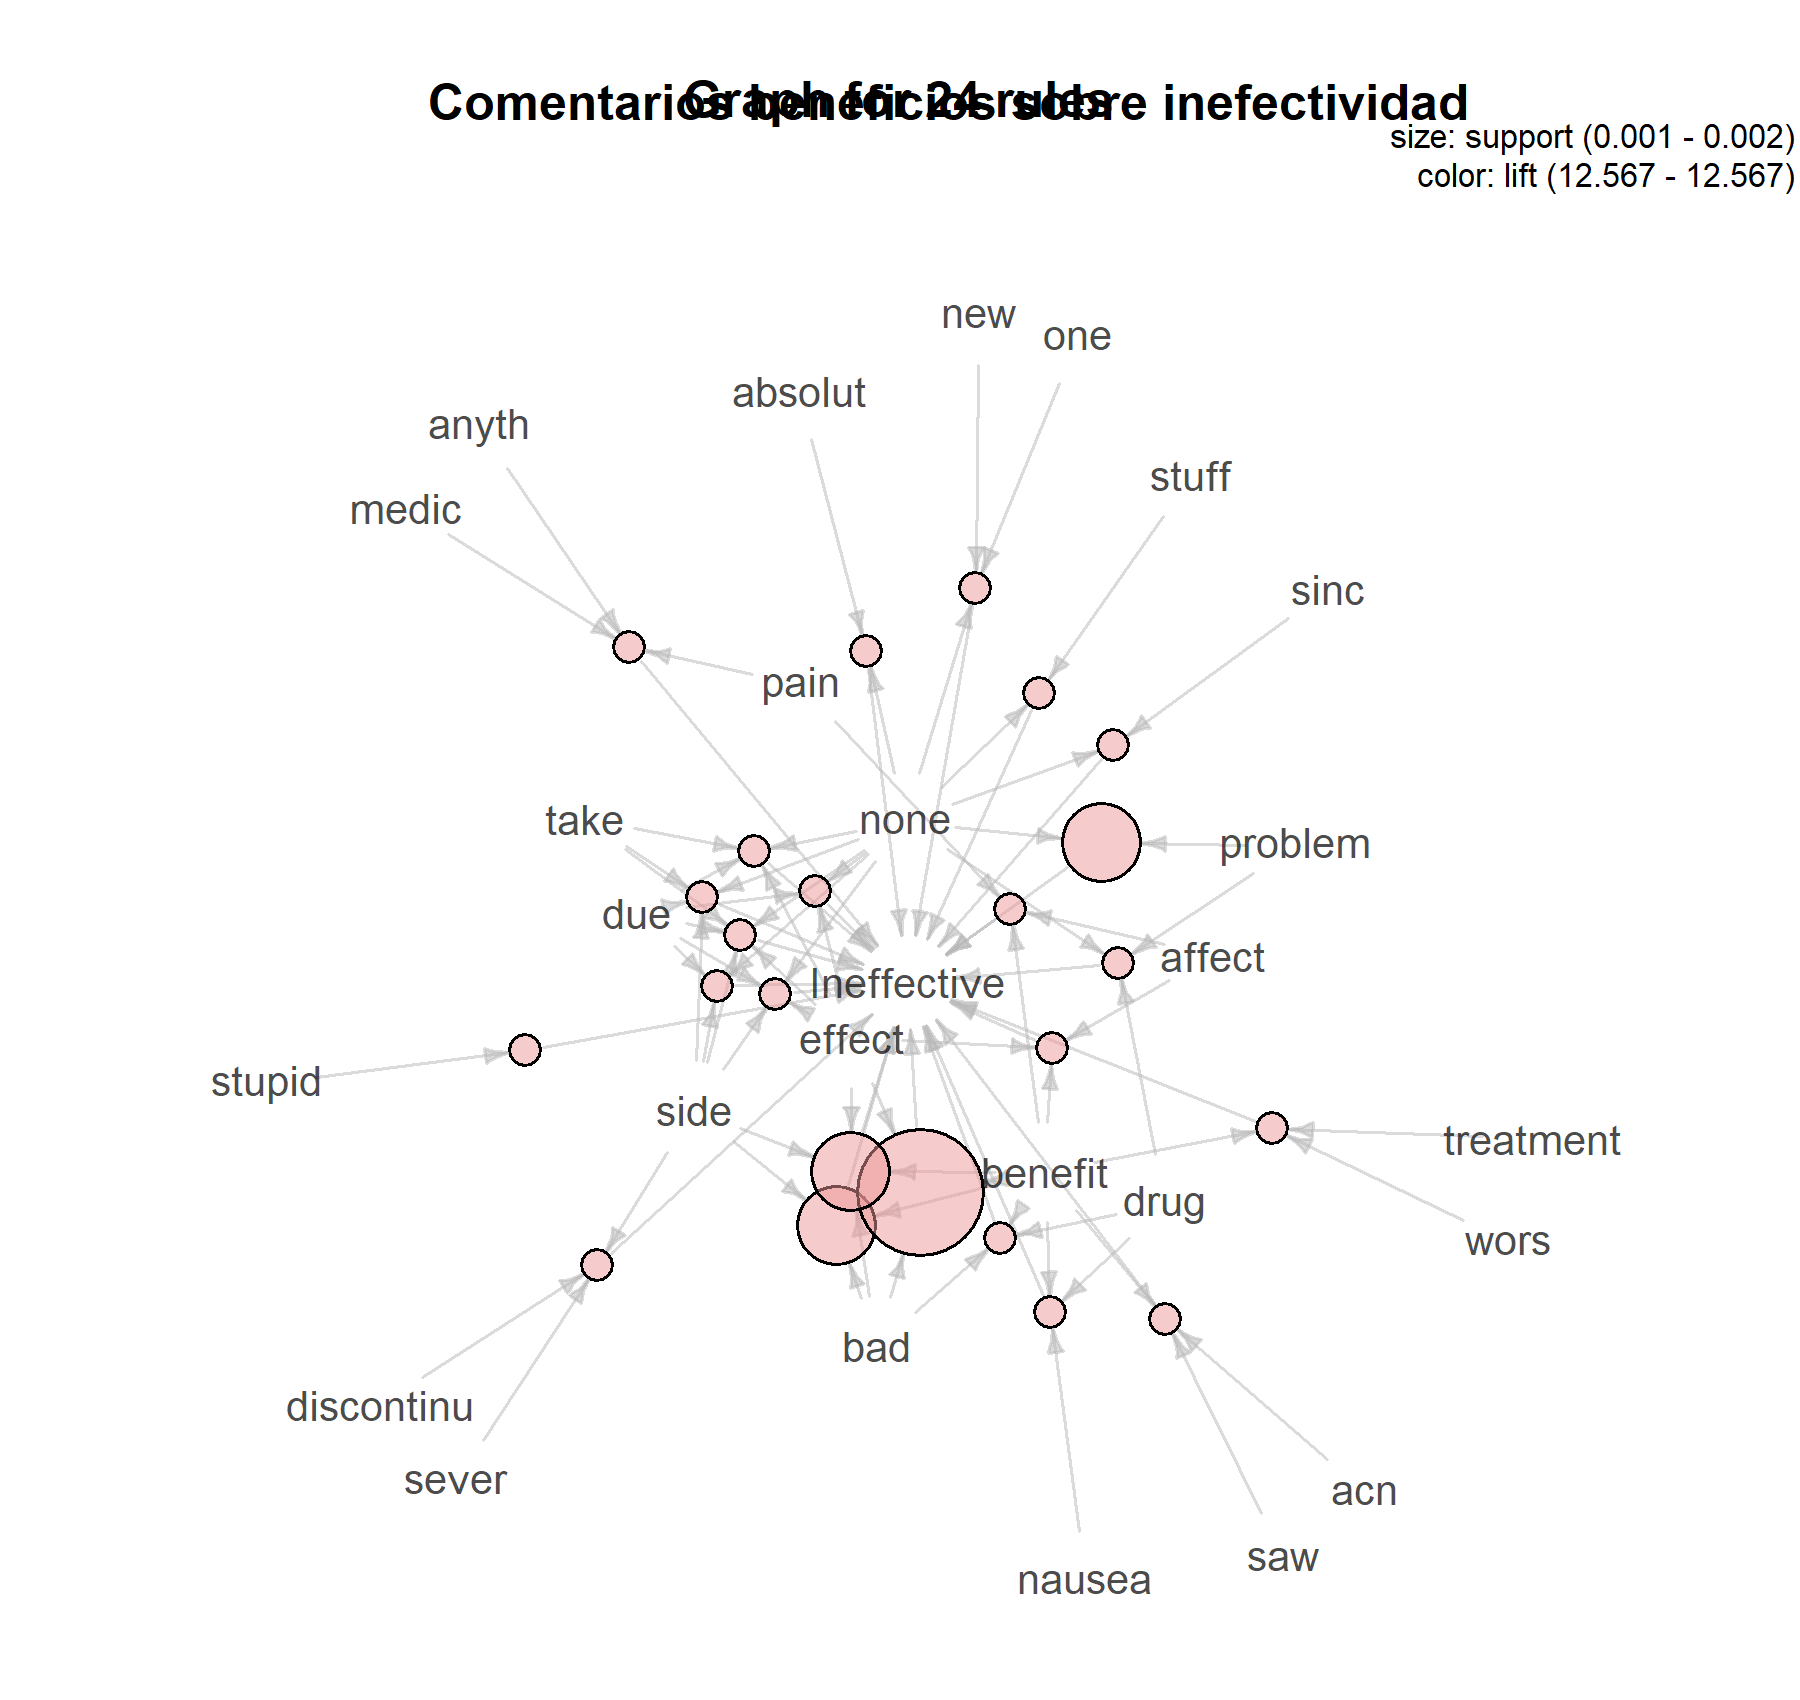
\includegraphics[width=1\textwidth]{figuras/asociacion/benefits_Innefective.png}
    \caption{Mapa de reglas de asociación con Innefective en el consecuente en comentarios sobre beneficios.}
    \label{fig:asociacion:innefectiveAsociacion}
\end{figure}

Como se puede ver en la imagen, los términos que giran en torno de a la
inefectividad tienen bastante sentido. Por ejemplo, la palabra
\emph{none}. Lo normal es que, cuando un medicamente es inefectivo, las
personas realicen comentarios del estilo ``no me ha hecho nada'' o ``no
sirve de nada''. Otros como \emph{pain} o \emph{problem} tienen sentido
ya que si un medicamento es inefectivo es normal que aparezcan palabras
``negativas''.

\begin{Shaded}
\begin{Highlighting}[]
\CommentTok{# Obtenemos las imágenes relacionadas con los comentarios }
\CommentTok{# sobre efectos secundarios de los medicamentos}
\KeywordTok{png}\NormalTok{(}\StringTok{"figuras/asociacion/effects_Innefective.png"}\NormalTok{,}\DataTypeTok{width=}\DecValTok{1800}\NormalTok{,}
    \DataTypeTok{height=}\DecValTok{1700}\NormalTok{,}\DataTypeTok{units=}\StringTok{"px"}\NormalTok{,}\DataTypeTok{pointsize=}\DecValTok{10}\NormalTok{,}\DataTypeTok{bg=}\StringTok{"white"}\NormalTok{,}\DataTypeTok{res=}\DecValTok{300}\NormalTok{)}
\KeywordTok{plot}\NormalTok{(effects_rulesInnefective, }\DataTypeTok{method=}\StringTok{"graph"}\NormalTok{)}
\KeywordTok{title}\NormalTok{(}\StringTok{"Comentarios efectos secundarios sobre inefectividad"}\NormalTok{)}
\KeywordTok{dev.off}\NormalTok{()}

\KeywordTok{png}\NormalTok{(}\StringTok{"figuras/asociacion/effects_HighlyEffective.png"}\NormalTok{,}\DataTypeTok{width=}\DecValTok{1800}\NormalTok{,}
    \DataTypeTok{height=}\DecValTok{1700}\NormalTok{,}\DataTypeTok{units=}\StringTok{"px"}\NormalTok{,}\DataTypeTok{pointsize=}\DecValTok{10}\NormalTok{,}\DataTypeTok{bg=}\StringTok{"white"}\NormalTok{,}\DataTypeTok{res=}\DecValTok{300}\NormalTok{)}
\KeywordTok{plot}\NormalTok{(effects_rulesHighlyEffective, }\DataTypeTok{method=}\StringTok{"graph"}\NormalTok{)}
\KeywordTok{title}\NormalTok{(}\StringTok{"Comentarios efectos secundarios sobre altamente efectivos"}\NormalTok{)}
\KeywordTok{dev.off}\NormalTok{()}

\KeywordTok{png}\NormalTok{(}\StringTok{"figuras/asociacion/effects_ConsiderablyEffective.png"}\NormalTok{,}\DataTypeTok{width=}\DecValTok{1800}\NormalTok{,}
    \DataTypeTok{height=}\DecValTok{1700}\NormalTok{,}\DataTypeTok{units=}\StringTok{"px"}\NormalTok{,}\DataTypeTok{pointsize=}\DecValTok{10}\NormalTok{,}\DataTypeTok{bg=}\StringTok{"white"}\NormalTok{,}\DataTypeTok{res=}\DecValTok{300}\NormalTok{)}
\KeywordTok{plot}\NormalTok{(effects_rulesConsiderablyEffective, }\DataTypeTok{method=}\StringTok{"graph"}\NormalTok{)}
\KeywordTok{title}\NormalTok{(}\StringTok{"Comentarios efectos secundarios sobre considerablemente efectivos"}\NormalTok{)}
\KeywordTok{dev.off}\NormalTok{()}

\KeywordTok{png}\NormalTok{(}\StringTok{"figuras/asociacion/effects_ModeratelyEffective.png"}\NormalTok{,}\DataTypeTok{width=}\DecValTok{1800}\NormalTok{,}
    \DataTypeTok{height=}\DecValTok{1700}\NormalTok{,}\DataTypeTok{units=}\StringTok{"px"}\NormalTok{,}\DataTypeTok{pointsize=}\DecValTok{10}\NormalTok{,}\DataTypeTok{bg=}\StringTok{"white"}\NormalTok{,}\DataTypeTok{res=}\DecValTok{300}\NormalTok{)}
\KeywordTok{plot}\NormalTok{(effects_rulesModeratelyEffective, }\DataTypeTok{method=}\StringTok{"graph"}\NormalTok{)}
\KeywordTok{title}\NormalTok{(}\StringTok{"Comentarios efectos secundarios sobre moderadamente efectivos"}\NormalTok{)}
\KeywordTok{dev.off}\NormalTok{()}

\KeywordTok{png}\NormalTok{(}\StringTok{"figuras/asociacion/effects_MarginallyEffective.png"}\NormalTok{,}\DataTypeTok{width=}\DecValTok{1800}\NormalTok{,}
    \DataTypeTok{height=}\DecValTok{1700}\NormalTok{,}\DataTypeTok{units=}\StringTok{"px"}\NormalTok{,}\DataTypeTok{pointsize=}\DecValTok{10}\NormalTok{,}\DataTypeTok{bg=}\StringTok{"white"}\NormalTok{,}\DataTypeTok{res=}\DecValTok{300}\NormalTok{)}
\KeywordTok{plot}\NormalTok{(effects_rulesMarginallyEffective, }\DataTypeTok{method=}\StringTok{"graph"}\NormalTok{)}
\KeywordTok{title}\NormalTok{(}\StringTok{"Comentarios efectos secundarios sobre casi inefectivo"}\NormalTok{)}
\KeywordTok{dev.off}\NormalTok{()}
\end{Highlighting}
\end{Shaded}

Sobre los comentarios de efectos secundarios podemos analizar, por
ejemplo, el concepto de altamente efectivo:

\begin{figure}[h]
    \centering
    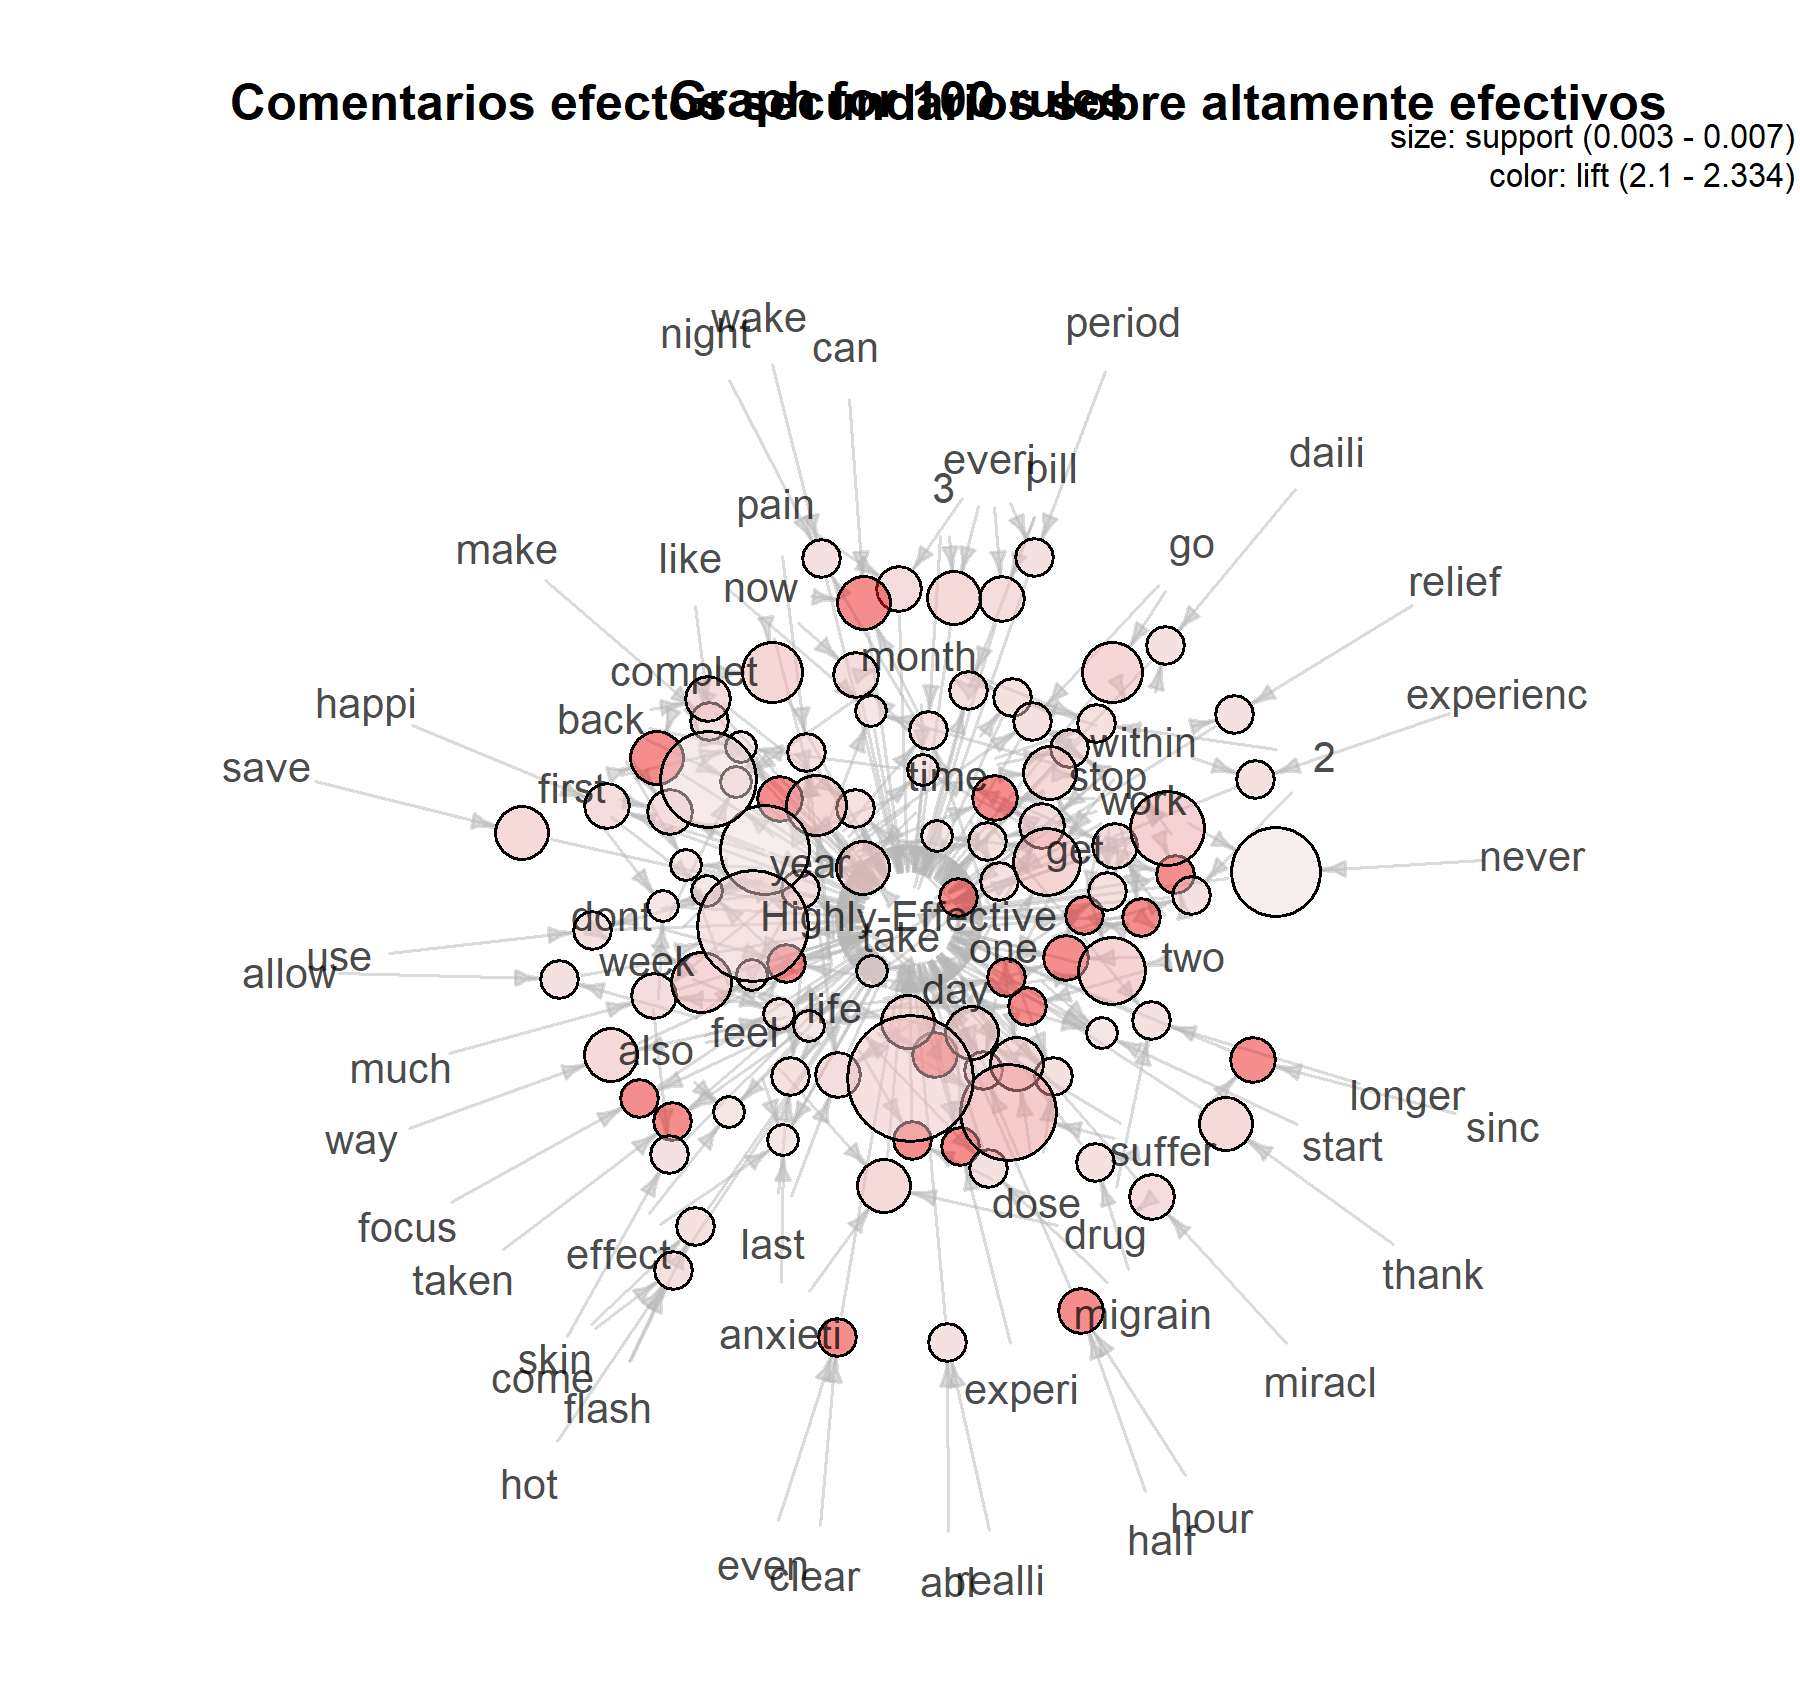
\includegraphics[width=1\textwidth]{figuras/asociacion/effects_HighlyEffective.png}
    \caption{Mapa de reglas de asociación con Highly-Effective en el consecuente en comentarios sobre efectos secundarios.}
    \label{fig:asociacion:innefectiveAsociacion}
\end{figure}

Como podemos apreciar en la imagen, el mapa de por sí es poco
visualizable debido a la cantidad de reglas que aparecen en tan poco
espacio. En definitiva, si nos fijamos bien podemos darnos cuenta de que
tiene bastante sentido.

\newpage

\section{6. Agrupamiento y Clustering}\label{agrupamiento-y-clustering}

Para la realización del Clustering, se debe destacar el uso de este
\href{https://rpubs.com/Joaquin_AR/310338}{enlace}.

\subsection{6.1. Introducción}\label{introduccion}

En el siguiente capítulo nos enfrentamos al desarrollo de la
clasificación no supervisada de patrones en grupos, mas conocido como
clustering. Dichos grupos se establecen como particiones en las que las
observaciones pertenecientes son similares entre ellas y distintas a las
observaciones del resto de particiones.

Debido a la naturaleza de nuestros datos, y la estructuración que hemos
hecho para su tratamiento, tenemos tanto datos numéricos
(correspondientes a valores de distintas puntuaciones asignadas a los
agrupamientos), como datos textuales. Por ello, vamos a dividir esta
sección en dos problemas, que se tratarán de forma separada.

\begin{itemize}
\item
  \textbf{Agrupamiento de los fármacos en base a las puntuaciones obtenidas}.
  En este caso, tendremos en cuenta los distintos atributos numéricos
  que nos dan información acerca de las opiniones del fármaco, y los
  utilizaremos para realizar dicha clasificación. Estos atributos son
  \emph{rating}, \emph{effectivenessNumber} y \emph{sideEffectsInverse}.
\item
  \textbf{Agrupamiento de los fármacos en base a las opiniones de los usuarios}.
  Para este apartado, realizaremos, en primer lugar, un agrupamiento en
  base a \emph{benefitsReview}, y por otra parte, en función de
  \emph{sideEffectsReview}.
\end{itemize}

Para los distintos apartados, se estudiarán distintas técnicas de
agrupamiento, con la explicación y comparación correspondiente de
nuestros resultados, para así poder ver su utilidad y adecuación de la
técnica en base a las características de los datos que estamos tratando
(puesto que habrá técnicas que, debido a la naturaleza de nuestors
datos, sean más apropiadas que otras). En esta sección se verá, como se
ha comentado en capítulos previos, que en nuestra base de datos existe
un alto factor de subjetividad, que influirá en nuestros resultados.

\subsection{6.2. Agrupamiento de los fármacos en base a las puntuaciones
obtenidas}\label{agrupamiento-de-los-farmacos-en-base-a-las-puntuaciones-obtenidas}

\subsubsection{6.2.1. Establecimiento de una
semilla}\label{establecimiento-de-una-semilla}

Como esta técnica tiene un factor de aleatoriedad, lo primero que vamos
a hacer es establecer una semilla común, para así poder replicar los
resultados en las distintas ejecuciones futuras que queramos realizar.

\subsubsection{6.2.2. Lectura y adecuación de los
datos}\label{lectura-y-adecuacion-de-los-datos}

Como proceso anterior al punto en el que nos encontramos, se realizó
todo el preprocesado de los datos. Ahora, para su uso en las técnicas de
clustering, debemos tomar las columnas de datos que más nos interesan
para el análisis.

Como ya se comentó en la introducción de este capítulo, estas serán
\emph{rating}, \emph{effectivenessNumber} y \emph{sideEffectsInverse}.
Por ello, tras leer los datos, lo primero que vamos a hacer, es crear un
nuevo data-frame de la forma específica que necesitamos que estén los
datos para esta técnica en concreto. Si consultamos el data-frame
original, las variables que necesitamos se corresponde con las columnas
número 2, 12 y 19 respectivamente, y estas serán por tanto, las que
filtraremos para el nuevo conjunto de datos con el que vamos a trabajar.

\begin{Shaded}
\begin{Highlighting}[]
\CommentTok{# Establecemos una semilla para obtener siempre los mismos resultados}
\KeywordTok{set.seed}\NormalTok{(}\DecValTok{3}\NormalTok{)}

\CommentTok{# Cargamos los datos}
\NormalTok{datos_train <-}\StringTok{ }\KeywordTok{read.table}\NormalTok{(}\StringTok{"datos/datos_train_preprocesado.csv"}\NormalTok{, }\DataTypeTok{sep=}\StringTok{","}\NormalTok{, }
                          \DataTypeTok{comment.char=}\StringTok{""}\NormalTok{,}\DataTypeTok{quote =} \StringTok{"}\CharTok{\textbackslash{}"}\StringTok{"}\NormalTok{, }\DataTypeTok{header=}\OtherTok{TRUE}\NormalTok{)}

\NormalTok{datos_test <-}\StringTok{ }\KeywordTok{read.table}\NormalTok{(}\StringTok{"datos/datos_test_preprocesado.csv"}\NormalTok{, }\DataTypeTok{sep=}\StringTok{","}\NormalTok{, }
                         \DataTypeTok{comment.char=}\StringTok{""}\NormalTok{,}\DataTypeTok{quote =} \StringTok{"}\CharTok{\textbackslash{}"}\StringTok{"}\NormalTok{, }\DataTypeTok{header=}\OtherTok{TRUE}\NormalTok{)}

\CommentTok{# Nos quedamos con las columnas que nos interesan }
\CommentTok{# Las columnas que tenemos son: RATING, SIDE_EFFECTS_INVERSE, EFFECTIVENESS_NUMBER}
\NormalTok{datos_train2 =}\StringTok{ }\NormalTok{datos_train[}\KeywordTok{c}\NormalTok{(}\DecValTok{2}\NormalTok{,}\DecValTok{12}\NormalTok{,}\DecValTok{9}\NormalTok{)]}
\NormalTok{datos_test2 =}\StringTok{ }\NormalTok{datos_test[}\KeywordTok{c}\NormalTok{(}\DecValTok{2}\NormalTok{,}\DecValTok{12}\NormalTok{,}\DecValTok{9}\NormalTok{)]}
\end{Highlighting}
\end{Shaded}

A continuación, podemos ver la estructura que estamos utilizando para el
conjunto de train.

\begin{Shaded}
\begin{Highlighting}[]
\KeywordTok{head}\NormalTok{(datos_train2)}
\end{Highlighting}
\end{Shaded}

\begin{verbatim}
##   rating sideEffectsInverse effectivenessNumber
## 1      4                  4                   5
## 2      1                  2                   5
## 3     10                  5                   5
## 4      3                  4                   2
## 5      2                  2                   2
## 6      1                  2                   1
\end{verbatim}

Como ya sabemos, todos aquellos cambios que realicemos en train, tienen
que ser replicados para el conjunto de test. Como se puede ver a
continuación, se ha realizado este cambio.

\begin{Shaded}
\begin{Highlighting}[]
\KeywordTok{head}\NormalTok{(datos_test2)}
\end{Highlighting}
\end{Shaded}

\begin{verbatim}
##   rating sideEffectsInverse effectivenessNumber
## 1      9                  4                   4
## 2      9                  4                   5
## 3      4                  2                   3
## 4     10                  5                   5
## 5     10                  4                   5
## 6      2                  5                   2
\end{verbatim}

Sin embargo, esta selección inicial de columnas no es suficiente para
poder empezar a aplicar las técnicas, ya que, a pesar de que nos hemos
quedado con los atributos que necesitamos para dicho agrupamiento, esta
estructura tiene deficiencias:

\begin{itemize}
\tightlist
\item
  En primer lugar, hemos perdido el nombre de los medicamentos de
  nuestro conjunto de datos. Con esto queremos decir que, con el dataset
  que tenemos actualmente, no sabemos el nombre del fármaco que se
  asocia a cada fila. Esto es importante a la hora de visualizar el
  agrupamiento, ya que, la única manera de ver qué fármacos aparecen en
  cada clúster que visualicemos, es asociándole etiquetas. De dicha
  forma, podremos ver con qué fármaco se corresponde cada item de la
  gráfica.
\end{itemize}

Como solución a este problema, vamos a renombrar las filas del dataset,
de forma que cada fila tenga como nombre el del fármaco correspondiente.
Esto tiene un problema, y es que en un hipotético caso en el que
tuviéramos varios comentarios para un mismo fármaco, no podríamos
realizar este cambio de nombres, puesto que dos filas de un mismo
dataset no pueden tener el mismo nombre. Con esta reflexión, nos surge
un nuevo problema, y es que, no queremos que el mismo fármaco salga en
distintos agrupamientos. Lo que nos parece más coherente es, que se
agrupen los fármacos, de forma que cada uno de los fármacos pertenezca a
un clúster. La idea general a la que pretendemos llegar, es a obtener
distintas agrupaciones de fármacos en base a sus características.
Tenemos dos formas de obtener un dataset donde cada fila sea un fármaco:

\begin{itemize}
\item
  En el caso de que tengamos \emph{x} items asociados a un mismo fármaco
  (varios comentarios respecto a un único fármaco), \emph{quedarnos
  únicamente con un item}. Esta solución no nos pareció la más adecuada,
  puesto que \textbf{estaríamos perdiendo información}.
\item
  \emph{Realizar alguna medida estadística que nos permita agregar dicha
  información}. Como estuvimos observando que las opiniones respecto a
  los fármacos suelen coincidir cuando hay más de una, esta opción fue
  la que vimos menos problemática (aunque como ya sabemos, estaríamos
  perdiendo algo de información igualmente), y por tanto la que
  utilizaremos en esta sección.
\end{itemize}

\begin{Shaded}
\begin{Highlighting}[]
\CommentTok{# Arreglamos el conjunto de datos para poder trabajar con lo que nos interesa}

\CommentTok{# Obtenemos en una variable todos los nombres de fármacos que existen en el conjunto de train}
\NormalTok{nombres_farmacos_train <-}\StringTok{ }\KeywordTok{unique}\NormalTok{(datos_train[,}\DecValTok{1}\NormalTok{])}

\CommentTok{# Hacemos lo mismo para test}
\NormalTok{nombres_farmacos_test <-}\StringTok{ }\KeywordTok{unique}\NormalTok{(datos_test[,}\DecValTok{1}\NormalTok{])}

\CommentTok{# Creamos una matriz (vacía) con tantas filas como fármacos haya, y tantas columnas como }
\CommentTok{#atributos queramos utilizar. En este caso son 3 columnas porque necesitamos guardar la }
\CommentTok{#info de "rating", "sideEffectsInverse" y "effectivenessNumber".}
\NormalTok{datos_procesados_train <-}\StringTok{ }\KeywordTok{matrix}\NormalTok{(}\DataTypeTok{ncol=}\DecValTok{3}\NormalTok{, }\DataTypeTok{nrow=}\KeywordTok{length}\NormalTok{(nombres_farmacos_train))}
\NormalTok{datos_procesados_test <-}\StringTok{ }\KeywordTok{matrix}\NormalTok{(}\DataTypeTok{ncol=}\DecValTok{3}\NormalTok{, }\DataTypeTok{nrow=}\KeywordTok{length}\NormalTok{(nombres_farmacos_test))}


\CommentTok{# Primero procesamos TRAIN}

\CommentTok{# Convertimos la estructura que tiene todos los nombres de los fármacos, en un data-frame, }
\CommentTok{# para poder trabajar con esta información de manera más cómoda}
\NormalTok{df_farmacos_train =}\StringTok{ }\KeywordTok{as.data.frame}\NormalTok{(nombres_farmacos_train)}

\CommentTok{# Para cada uno de los fármacos existentes, vamos a guardar su información asociada en }
\CommentTok{# la matriz creada anteriormente}
\ControlFlowTok{for}\NormalTok{(i }\ControlFlowTok{in} \DecValTok{0}\OperatorTok{:}\KeywordTok{length}\NormalTok{(nombres_farmacos_train))\{}
  
  \CommentTok{# Obtenemos todas las filas del dataset que se correspondan con el fármaco número i.}
\NormalTok{  filas_farmaco_train <-}\StringTok{ }\NormalTok{datos_train2[}\KeywordTok{which}\NormalTok{(datos_train}\OperatorTok{$}\NormalTok{urlDrugName }\OperatorTok{==}\StringTok{ }\NormalTok{nombres_farmacos_train[i]),]}

  \CommentTok{# Como pueden ser más de una fila, resumimos dicha información.}
\NormalTok{  mean_rating_train <-}\StringTok{ }\KeywordTok{mean}\NormalTok{(filas_farmaco_train}\OperatorTok{$}\NormalTok{rating)}
\NormalTok{  mean_side_effect_train <-}\StringTok{ }\KeywordTok{mean}\NormalTok{(filas_farmaco_train}\OperatorTok{$}\NormalTok{sideEffectsInverse)}
\NormalTok{  mean_effectiveness_train <-}\StringTok{ }\KeywordTok{mean}\NormalTok{(filas_farmaco_train}\OperatorTok{$}\NormalTok{effectivenessNumber)}

  \CommentTok{# La información resumida es la que asociamos a dicho fármaco, montando la fila de la }
  \CommentTok{# manera adecuada. Nótese que redondeamos el número medio obtenido para sideEffects y}
  \CommentTok{# effectivenessNumber. Esto es porque necesitamos que sea un número entero (recordemos}
  \CommentTok{# que estos dos valores se corresponden con etiquetas).}
\NormalTok{  datos_procesados_train[i,] <-}\StringTok{ }\KeywordTok{c}\NormalTok{(mean_rating_train, }\KeywordTok{round}\NormalTok{(mean_side_effect_train),}
                                  \KeywordTok{round}\NormalTok{(mean_effectiveness_train))}
\NormalTok{\}}

\CommentTok{# Procesamos }\AlertTok{TEST}\CommentTok{ de forma análoga a TRAIN.}
\NormalTok{df_farmacos_test =}\StringTok{ }\KeywordTok{as.data.frame}\NormalTok{(nombres_farmacos_test)}

\ControlFlowTok{for}\NormalTok{(i }\ControlFlowTok{in} \DecValTok{0}\OperatorTok{:}\KeywordTok{length}\NormalTok{(nombres_farmacos_test))\{}
  
\NormalTok{  filas_farmaco_test <-}\StringTok{ }\NormalTok{datos_test2[}\KeywordTok{which}\NormalTok{(datos_test}\OperatorTok{$}\NormalTok{urlDrugName }\OperatorTok{==}\StringTok{ }\NormalTok{nombres_farmacos_test[i]),]}

\NormalTok{  mean_rating_test <-}\StringTok{ }\KeywordTok{mean}\NormalTok{(filas_farmaco_test}\OperatorTok{$}\NormalTok{rating)}
\NormalTok{  mean_side_effect_test <-}\StringTok{ }\KeywordTok{mean}\NormalTok{(filas_farmaco_test}\OperatorTok{$}\NormalTok{sideEffectsInverse)}
\NormalTok{  mean_effectiveness_test <-}\StringTok{ }\KeywordTok{mean}\NormalTok{(filas_farmaco_test}\OperatorTok{$}\NormalTok{effectivenessNumber)}

\NormalTok{  datos_procesados_test[i,] <-}\StringTok{ }\KeywordTok{c}\NormalTok{(mean_rating_test, }\KeywordTok{round}\NormalTok{(mean_side_effect_test), }\KeywordTok{round}\NormalTok{(mean_effectiveness_test))}
  
\NormalTok{\}}

\CommentTok{# Por último, convertimos las matrices procesadas anteriormente en data-frame}
\NormalTok{data_train_procesado <-}\StringTok{ }\KeywordTok{data.frame}\NormalTok{(datos_procesados_train)}
\NormalTok{data_test_procesado <-}\StringTok{ }\KeywordTok{data.frame}\NormalTok{(datos_procesados_test)}

\CommentTok{# Una vez creados los data-frame, les asignamos nombres a las filas y columnas de }
\CommentTok{# los nuevos data-frames.}
\KeywordTok{rownames}\NormalTok{(data_train_procesado) <-}\StringTok{ }\NormalTok{nombres_farmacos_train}
\KeywordTok{rownames}\NormalTok{(data_test_procesado) <-}\StringTok{ }\NormalTok{nombres_farmacos_test}
\KeywordTok{colnames}\NormalTok{(data_train_procesado) <-}\StringTok{ }\KeywordTok{c}\NormalTok{(}\StringTok{"rating"}\NormalTok{, }\StringTok{"sideEffectsInverse"}\NormalTok{, }\StringTok{"effectivenessNumber"}\NormalTok{)}
\KeywordTok{colnames}\NormalTok{(data_test_procesado) <-}\StringTok{ }\KeywordTok{c}\NormalTok{(}\StringTok{"rating"}\NormalTok{, }\StringTok{"sideEffectsInverse"}\NormalTok{, }\StringTok{"effectivenessNumber"}\NormalTok{)}
\end{Highlighting}
\end{Shaded}

A continuación se puede visualizar parte del nuevo data-frame que hemos
creado para el conjunto de train.

\begin{Shaded}
\begin{Highlighting}[]
\KeywordTok{head}\NormalTok{(data_train_procesado)}
\end{Highlighting}
\end{Shaded}

\begin{verbatim}
##                     rating sideEffectsInverse effectivenessNumber
## enalapril         5.000000                  4                   4
## ortho-tri-cyclen  7.437500                  4                   4
## ponstel          10.000000                  5                   5
## prilosec          7.000000                  4                   4
## lyrica            5.523810                  3                   3
## propecia          6.684211                  4                   4
\end{verbatim}

A continuación se puede visualizar parte del nuevo data-frame que hemos
creado para el conjunto de test.

\begin{Shaded}
\begin{Highlighting}[]
\KeywordTok{head}\NormalTok{(data_test_procesado)}
\end{Highlighting}
\end{Shaded}

\begin{verbatim}
##               rating sideEffectsInverse effectivenessNumber
## biaxin         5.000                  3                   4
## lamictal       8.300                  4                   4
## depakene       4.000                  2                   3
## sarafem        8.500                  4                   4
## accutane       7.375                  3                   4
## carbamazepine  8.000                  3                   4
\end{verbatim}

\textbf{Estos dos conjuntos de datos son con los que trabajaremos en el
resto de técnicas asociadas a agrupamiento de items, que realizaremos a
lo largo de este apartado. }

\subsubsection{6.2.3. K-medias}\label{k-medias}

La idea básica del presente método es agrupar las observaciones en K
clusters distintos, siendo el valor de K preestablecido mediante
análisis previos. Entonces, K-medias encuentra los K mejores clusters,
siendo estos aquellos cuya varianza interna sea lo más pequeña posible.

Como queremos, al fin y al cabo, agrupar los fármacos en función de los
datos, vamos a comenzar por lo más intuitivo posible. La primera
pregunta que nos surgió fue, ¿sería posible agrupar los fármacos en dos
clústers, de forma que tuvieramos un grupo para los fármacos ``buenos''
(aquellos que tienen una puntuación alta) y otro grupo para los fármacos
``malos'' (aquellos inefectivos, con efectos secundarios)?. En un primer
lugar puede parecer, que la agrupación resultante no tiene que ser
coherente en cuanto a lo que nosotros buscamos encontrar, puesto que al
fin y al cabo, son datos, y como hemos dicho anteriormente tenemos un
gran factor de subjetividad. Pero, observando nuestros datos, nos dimos
cuenta de una cosa, y es que, cuando alguien tenía una buena opinión
acerca de un fármaco, le asignaba a éste un alto valor de
\emph{effectiveness} y un alto bajo valor en \emph{sideEffects}, lo que,
a priori, es totalmente lógico e intuitivo.

Puesto que los datos que estamos utilizando en el conjunto de train, son
efectivamente esos, cabe esperar que sí podamos obtener una
clasificación respecto a fármacos cuya opinión es posivitiva, y fármacos
con opinión negativa. Siguiendo esta idea, vamos a probar a establecer
un número de cluster igual a 2 (K=2), y posteriormente, intentaremos
buscar un sentido a las agrupaciones que encontremos, ya que, al tener
únicamente dos grupos, nos resultará sencillo.

Para ello, utilizaremos la función \texttt{kmeans}, que nos permitirá
obtener la agrupación que hemos estado comentando anteriormente. Como
parámetros, mencionar, que hemos establecido el número de clústers a 2
(tal y como hemos expuesto en el párrafo anterior), y que la distancia
que utilizaremos en el algoritmo será la distancia \emph{euclídea}. En
la siguiente imagen, podemos ver el resultado alcanzado en este caso.
Aunque resulta poco visible debido a la gran cantidad de información que
hay en ella, podemos ver cómo prácticamente el espacio está dividido en
dos clústeres, medianamente bien predefinidos.

\begin{Shaded}
\begin{Highlighting}[]
\CommentTok{# ALgoritmo K-means con los datos de test y 2 clusters}
\NormalTok{res_clustering <-}\StringTok{ }\KeywordTok{kmeans}\NormalTok{(data_train_procesado, }\DecValTok{2}\NormalTok{)}

\CommentTok{# Lo mostramos}
\KeywordTok{fviz_cluster}\NormalTok{(}\DataTypeTok{object =}\NormalTok{ res_clustering, }\DataTypeTok{data =}\NormalTok{ data_train_procesado, }\DataTypeTok{show.clust.cent =} \OtherTok{TRUE}\NormalTok{,}
             \DataTypeTok{ellipse.type =} \StringTok{"euclid"}\NormalTok{, }\DataTypeTok{star.plot =} \OtherTok{TRUE}\NormalTok{, }\DataTypeTok{repel =} \OtherTok{TRUE}\NormalTok{, }\DataTypeTok{labelsize =} \DecValTok{9}\NormalTok{) }\OperatorTok{+}
\StringTok{  }\KeywordTok{labs}\NormalTok{(}\DataTypeTok{title =} \StringTok{"Resultados clustering K-means (con etiquetas)"}\NormalTok{) }\OperatorTok{+}
\StringTok{  }\KeywordTok{theme_bw}\NormalTok{() }\OperatorTok{+}
\StringTok{  }\KeywordTok{theme}\NormalTok{(}\DataTypeTok{legend.position =} \StringTok{"none"}\NormalTok{)}
\end{Highlighting}
\end{Shaded}

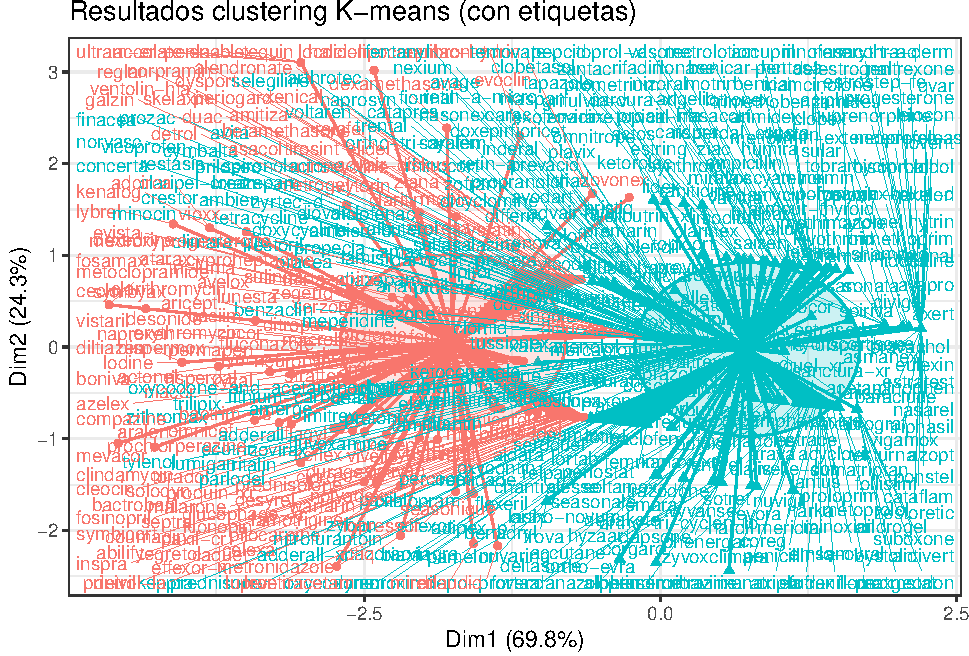
\includegraphics{practica-original_files/figure-latex/unnamed-chunk-153-1.pdf}
Intuitivamente, hemos intentado encontrar una relación entre los dos
agrupamientos, viendo que, efectivamente, con los distintos ejemplos que
hemos probado hemos podido ver, que los del grupo azul suelen tener una
efectividad entre 1 y 3, mientras que los del grupo rojo suelen tener
dicho valor entre 3 y 5. Idem para la variable de efectos secundarios,
lo que nos lleva a pensar que, realmente, hemos podido obtener una buena
clasificación de los fármacos en base a la opinión (positiva o negativa)
de los usuarios.

Véase por ejemplo, algunos ejemplos del grupo que se corresponde con el
color rojo en la gráfica. Como podemos ver, efectivamente su valor de
efectividad (cuarta columna en el dataset), tiene valor bajo. Además, si
miramos el valor en efectos secundarios, también es bajo (recordemos que
hicimos la inversa a dicho valor, y que cuanto más bajo sea el valor de
esa columna, más negativos son sus efectos).

\begin{Shaded}
\begin{Highlighting}[]
\NormalTok{train_medicine =}\StringTok{ }\KeywordTok{bind_cols}\NormalTok{(data_train_procesado,df_farmacos_train)}
\NormalTok{ejemplo1 <-}\StringTok{ }\NormalTok{train_medicine[}\KeywordTok{which}\NormalTok{(train_medicine}\OperatorTok{$}\NormalTok{nombres_farmacos_train }\OperatorTok{==}\StringTok{ "baciim"}\NormalTok{),]}
\NormalTok{ejemplo2 <-}\StringTok{ }\NormalTok{train_medicine[}\KeywordTok{which}\NormalTok{(train_medicine}\OperatorTok{$}\NormalTok{nombres_farmacos_train }\OperatorTok{==}\StringTok{ "boniva"}\NormalTok{),]}
\NormalTok{ejemplo3 <-}\StringTok{ }\NormalTok{train_medicine[}\KeywordTok{which}\NormalTok{(train_medicine}\OperatorTok{$}\NormalTok{nombres_farmacos_train }\OperatorTok{==}\StringTok{ "lodine"}\NormalTok{),]}
\NormalTok{ejemplo4 <-}\StringTok{ }\NormalTok{train_medicine[}\KeywordTok{which}\NormalTok{(train_medicine}\OperatorTok{$}\NormalTok{nombres_farmacos_train }\OperatorTok{==}\StringTok{ "mevacor"}\NormalTok{),]}

\NormalTok{pruebas_rojo =}\StringTok{ }\KeywordTok{bind_rows}\NormalTok{(ejemplo1,ejemplo2,ejemplo3,ejemplo4)}

\NormalTok{pruebas_rojo}
\end{Highlighting}
\end{Shaded}

\begin{verbatim}
##   rating sideEffectsInverse effectivenessNumber nombres_farmacos_train
## 1      5                  2                   1                 baciim
## 2      2                  2                   2                 boniva
## 3      1                  2                   2                 lodine
## 4      2                  1                   2                mevacor
\end{verbatim}

Hemos visto la tendencia. Ahora vamos a calcular, de forma media, el
valor asociado a effectivenessNumber en todos los fármacos que forman
parte de este primer cluster (el de color azul, el cuál se corresponde
con la etiqueta 1). Como se puede ver, el valor obtenido no llega a 3.

\begin{Shaded}
\begin{Highlighting}[]
\CommentTok{# Para poder obtener las etiquetas y fármacos asociados del objeto clúster, pasamos a matriz}
\NormalTok{m =}\StringTok{ }\KeywordTok{as.matrix}\NormalTok{(res_clustering}\OperatorTok{$}\NormalTok{cluster)}
\NormalTok{x=}\KeywordTok{as.matrix}\NormalTok{( m[,}\DecValTok{1}\NormalTok{] }\OperatorTok{==}\StringTok{ }\DecValTok{1}\NormalTok{)}

\CommentTok{# nos quedamos con los nombres de los fármacos que estén en el cluster 1}
\NormalTok{items_etiqueta1=}\StringTok{ }\NormalTok{x[,}\DecValTok{1}\NormalTok{]}\OperatorTok{==}\DecValTok{1}

\CommentTok{# nos quedamos con los fármacos del dataset que se correspondan con dicho cluster}
\NormalTok{farmacos_etiqueta1 =}\StringTok{ }\NormalTok{data_train_procesado[items_etiqueta1,]}

\CommentTok{# hacemos la media}
\KeywordTok{mean}\NormalTok{(farmacos_etiqueta1}\OperatorTok{$}\NormalTok{effectivenessNumber)}
\end{Highlighting}
\end{Shaded}

\begin{verbatim}
## [1] 2.972973
\end{verbatim}

Si ahora hacemos el mismo proceso para 4 fármacos del conjunto azul,
podemos ver que efectivamente, el comportamiento es el esperado. Tenemos
altos valores de efectividad, y pocos efectos secundarios.

\begin{Shaded}
\begin{Highlighting}[]
\NormalTok{ejemplo1 <-}\StringTok{ }\NormalTok{train_medicine[}\KeywordTok{which}\NormalTok{(train_medicine}\OperatorTok{$}\NormalTok{nombres_farmacos_train }\OperatorTok{==}\StringTok{ "zyvox"}\NormalTok{),]}
\NormalTok{ejemplo2 <-}\StringTok{ }\NormalTok{train_medicine[}\KeywordTok{which}\NormalTok{(train_medicine}\OperatorTok{$}\NormalTok{nombres_farmacos_train }\OperatorTok{==}\StringTok{ "bisoprolol"}\NormalTok{),]}
\NormalTok{ejemplo3 <-}\StringTok{ }\NormalTok{train_medicine[}\KeywordTok{which}\NormalTok{(train_medicine}\OperatorTok{$}\NormalTok{nombres_farmacos_train }\OperatorTok{==}\StringTok{ "cefzil"}\NormalTok{),]}
\NormalTok{ejemplo4 <-}\StringTok{ }\NormalTok{train_medicine[}\KeywordTok{which}\NormalTok{(train_medicine}\OperatorTok{$}\NormalTok{nombres_farmacos_train }\OperatorTok{==}\StringTok{ "benicar"}\NormalTok{),]}

\NormalTok{pruebas_azul =}\StringTok{ }\KeywordTok{bind_rows}\NormalTok{(ejemplo1,ejemplo2,ejemplo3,ejemplo4)}

\NormalTok{pruebas_azul}
\end{Highlighting}
\end{Shaded}

\begin{verbatim}
##   rating sideEffectsInverse effectivenessNumber nombres_farmacos_train
## 1      9                  3                   5                  zyvox
## 2     10                  5                   5             bisoprolol
## 3      8                  4                   4                 cefzil
## 4      9                  5                   4                benicar
\end{verbatim}

De nuevo, vamos a consultar el valor medio de efectividad que se
consigue si consultamos dicho atributo para todos los fármacos que se
han agrupado en el cluster que se corresponde con el color rojo en el
gráfico (grupo 2). Para ello, simplemente hacemos la media de todos
aquellos fármacos no incluidos en el grupo 1, y, tal y como es de
esperar, el resultado está entre 3 y 5, lo cuál nos \textbf{reafirma al
pensar que el agrupamiento se ha hecho en función de fármaco con opinión
positiva y fármaco con opinión negativa}.

\begin{Shaded}
\begin{Highlighting}[]
\NormalTok{farmacos_etiqueta2 =}\StringTok{ }\NormalTok{data_train_procesado[}\OperatorTok{-}\NormalTok{items_etiqueta1,]}
\KeywordTok{mean}\NormalTok{(farmacos_etiqueta2}\OperatorTok{$}\NormalTok{effectivenessNumber)}
\end{Highlighting}
\end{Shaded}

\begin{verbatim}
## [1] 3.894212
\end{verbatim}

Como aclaración, debido a la poca visibilidad del clúster, vamos a
mostrar el mismo gráfico, pero esta vez sin etiquetas, de forma que
podamos ver bien los agrupamientos que se llevan a cabo. Se puede
observar este hecho en la siguiente imagen del documento.

\begin{Shaded}
\begin{Highlighting}[]
\KeywordTok{fviz_cluster}\NormalTok{(}\DataTypeTok{object =}\NormalTok{ res_clustering, }\DataTypeTok{data =}\NormalTok{ data_train_procesado, }\DataTypeTok{show.clust.cent =} \OtherTok{TRUE}\NormalTok{,}
             \DataTypeTok{ellipse.type =} \StringTok{"euclid"}\NormalTok{, }\DataTypeTok{star.plot =} \OtherTok{TRUE}\NormalTok{, }\DataTypeTok{repel =} \OtherTok{TRUE}\NormalTok{, }\DataTypeTok{labelsize=}\DecValTok{0}\NormalTok{) }\OperatorTok{+}
\StringTok{  }\KeywordTok{labs}\NormalTok{(}\DataTypeTok{title =} \StringTok{"Resultados clustering K-means (sin etiquetas)"}\NormalTok{) }\OperatorTok{+}
\StringTok{  }\KeywordTok{theme_bw}\NormalTok{() }\OperatorTok{+}
\StringTok{  }\KeywordTok{theme}\NormalTok{(}\DataTypeTok{legend.position =} \StringTok{"none"}\NormalTok{)}
\end{Highlighting}
\end{Shaded}

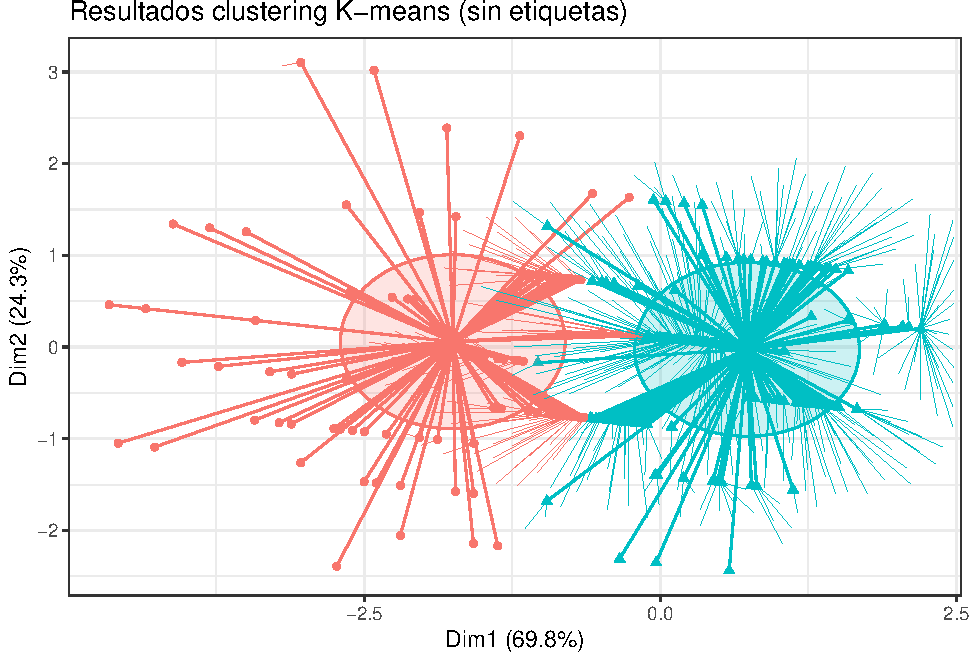
\includegraphics{practica-original_files/figure-latex/unnamed-chunk-158-1.pdf}
Sin embargo, tal y como ya se ha dicho, esto es una conclusión,
intuitiva, que hemos obtenido nosotros gracias a la gran cantidad de
información que nos ha dado el preprocesamiento y estudio exploratorio
de los datos.

Sin embargo, para validar nuestro modelo, podemos utilizar también algún
tipo de medida que nos permita saber cómo de bueno es el agrupamiento o
asignación que se ha llevado a cabo con la técnica. Para llevar a cabo
este procedimiento, vamos a utilizar una de las técnicas que hemos visto
en la asignatura: el método \emph{Average Siluette}. Para ello vamos a
utilizar lo que se denomina \emph{índice silueta}, el cuál es un
coeficiente que compara la distancia de un item con el resto de items,
ya sea del mismo cluster, o del resto de ellos. Se mueve en el rango
{[}-1,1{]}, de forma que, cuánto mayor sea el valor, mayor es su
adecuación en el agrupamiento realizado. A su vez, valores negativos
llevarán a pensar que se ha llevado a cabo una asignación incorrecta y
poco fiable. Este método es muy potente, ya que nos permite evaluar el
agrupamiento tanto a nivel de cada uno de los items, como a nivel de
clúster concreto, o a clústeres totales en el agrupamiento.

Teniendo en cuenta dicho índice, el número de clústers con el que se
obtendrían mejores resultados para el agrupamiento sería aquel
\textbf{cuya media del índice silueta fuese la mayor posible}. Podemos
ver el resultado de esta \emph{media}, para distintos tamaños de clúster
en la siguiente imagen. En la siguiente imagen, podemos ver, cómo en
este caso, el índice silueta indica que el número óptimo de clúster es
14. Pero sin embargo, tal y como ya sabemos, ese no tiene por qué ser el
más adecuado a usar, puesto que, en la práctica, también debemos de
tener en cuenta otras cuestiones que hemos visto en la asignatura, como
el esfuerzo computacional o el sobreaprendizaje que añadimos a nuestro
modelo cuando intentamos precisar demasiado. Al final, nos quedaremos
con un número de cluster que, nos permita una mejora sustancial, y a
partir del cuál no haya una mejora sustancial.

En dicha gráfica podemos ver que usar dos clusters tiene un valor alto
de índice medio de silueta, lo que nos hace pensar que, es un valor que
funciona bien y cuyo agrupamiento puede ser fiable (aspecto que ya
intuíamos).

\begin{Shaded}
\begin{Highlighting}[]
\CommentTok{# datos ya lo tenemos previamente escalado (K-medias)}
\NormalTok{datos <-}\StringTok{ }\KeywordTok{scale}\NormalTok{(data_train_procesado)}
\KeywordTok{fviz_nbclust}\NormalTok{(}\DataTypeTok{x =}\NormalTok{ datos, }\DataTypeTok{FUNcluster =}\NormalTok{ kmeans, }\DataTypeTok{method =} \StringTok{"silhouette"}\NormalTok{, }\DataTypeTok{k.max =} \DecValTok{15}\NormalTok{) }\OperatorTok{+}
\StringTok{  }\KeywordTok{labs}\NormalTok{(}\DataTypeTok{title =} \StringTok{"Número óptimo de clusters"}\NormalTok{)}
\end{Highlighting}
\end{Shaded}

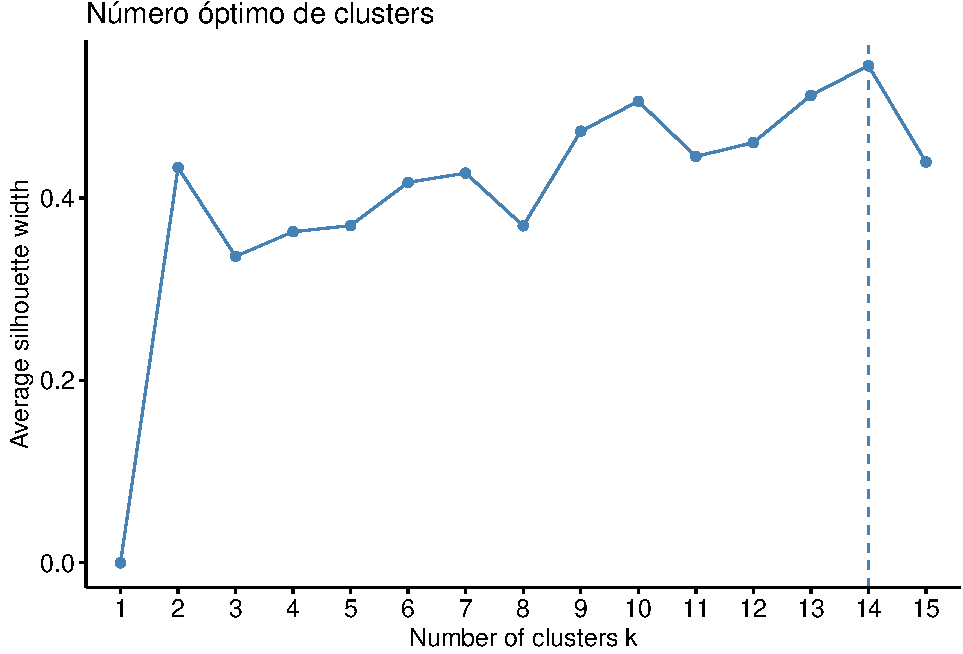
\includegraphics{practica-original_files/figure-latex/unnamed-chunk-159-1.pdf}

A su vez, podemos realizar una validación interna del clúster haciendo
uso del ya mencionado \emph{índice silueta}. Se puede visualizar el
resultado en la siguiente gráfica.

\begin{Shaded}
\begin{Highlighting}[]
\NormalTok{datos <-}\StringTok{ }\KeywordTok{scale}\NormalTok{(data_train_procesado)}
\NormalTok{km_clusters <-}\StringTok{ }\KeywordTok{eclust}\NormalTok{(}\DataTypeTok{x =}\NormalTok{ datos, }\DataTypeTok{FUNcluster =} \StringTok{"kmeans"}\NormalTok{, }\DataTypeTok{k =} \DecValTok{2}\NormalTok{, }\DataTypeTok{seed =} \DecValTok{123}\NormalTok{,}
                      \DataTypeTok{hc_metric =} \StringTok{"euclidean"}\NormalTok{, }\DataTypeTok{nstart =} \DecValTok{50}\NormalTok{, }\DataTypeTok{graph =} \OtherTok{FALSE}\NormalTok{)}
\KeywordTok{fviz_silhouette}\NormalTok{(}\DataTypeTok{sil.obj =}\NormalTok{ km_clusters, }\DataTypeTok{print.summary =} \OtherTok{TRUE}\NormalTok{, }\DataTypeTok{palette =} \StringTok{"jco"}\NormalTok{,}
                \DataTypeTok{ggtheme =} \KeywordTok{theme_classic}\NormalTok{()) }
\end{Highlighting}
\end{Shaded}

\begin{verbatim}
##   cluster size ave.sil.width
## 1       1  158          0.24
## 2       2  344          0.52
\end{verbatim}

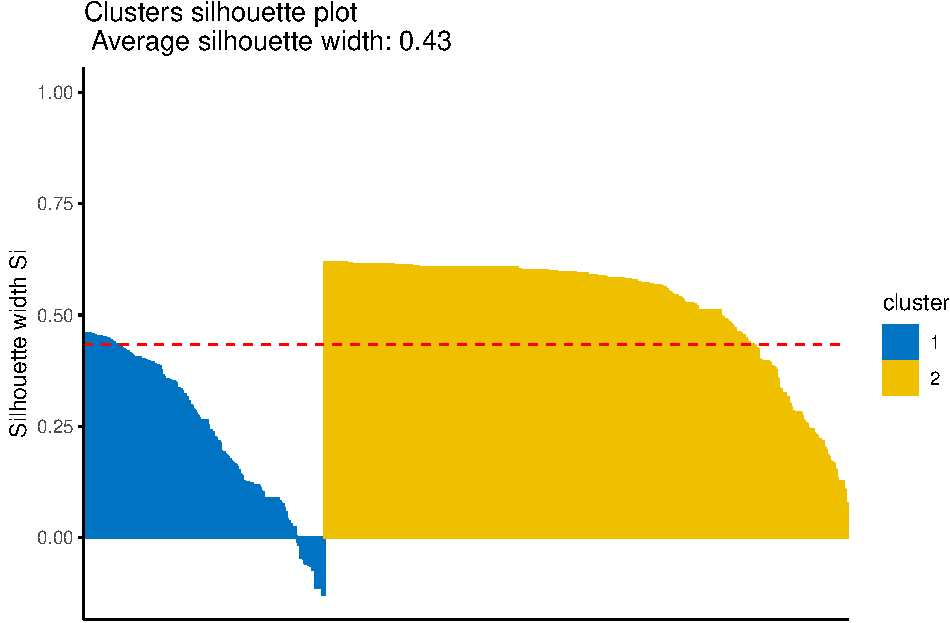
\includegraphics{practica-original_files/figure-latex/unnamed-chunk-160-1.pdf}
A su vez, podemos ver la media del índice silueta obtenida para cada uno
de los clusters, tal y como se puede ver a continuación. Como podemos
ver, la media obtenida para el primer cluster, es próxima a 0, lo que
nos puede indicar que los items no están en el grupo correcto. De hecho,
si observamos la gráfica anterior, podemos ver que algunos datos rozan
el negativo, y que se corresponderán a aquellos más próximos al otro
cluster.

\begin{Shaded}
\begin{Highlighting}[]
\CommentTok{# Media silhouette por cluster}
\NormalTok{km_clusters}\OperatorTok{$}\NormalTok{silinfo}\OperatorTok{$}\NormalTok{clus.avg.widths}
\end{Highlighting}
\end{Shaded}

\begin{verbatim}
## [1] 0.2357250 0.5238887
\end{verbatim}

En realidad, esto es normal que ocurra, sobretodo en nuestro caso,
puesto que:

\begin{enumerate}
\def\labelenumi{\arabic{enumi}.}
\item
  Es normal que algun valor concreto se escape, y no se agrupe bien,
  sobretodo cuando no hemos usado el valor óptimo de clusters.
\item
  Hay muchos items cuyo valor de effectiveness es 3. Recordemos que este
  valor se mueve en el rango {[}1,3{]}, por lo que, los items cuyo valor
  sea el valor medio, puede darse el caso de que sufran una mala
  clasificación. De hecho, podemos filtrar los índices silueta de
  nuestros items, tal y como se puede ver a continuación. De hecho, en
  la siguiente salida, podemos estos items, tienen un valor negativo muy
  muy muy cercano a 0, lo que hace más evidente dicha conclusión.
\end{enumerate}

\begin{Shaded}
\begin{Highlighting}[]
\NormalTok{km_clusters}\OperatorTok{$}\NormalTok{silinfo}\OperatorTok{$}\NormalTok{widths }\OperatorTok\StringTok{ }\KeywordTok{filter}\NormalTok{(sil_width }\OperatorTok{<=}\StringTok{ }\DecValTok{0}\NormalTok{)}
\end{Highlighting}
\end{Shaded}

\begin{verbatim}
##    cluster neighbor    sil_width
## 1        1        2 -0.008108751
## 2        1        2 -0.014884917
## 3        1        2 -0.043886193
## 4        1        2 -0.043886193
## 5        1        2 -0.046451962
## 6        1        2 -0.057008242
## 7        1        2 -0.057008242
## 8        1        2 -0.059306622
## 9        1        2 -0.059306622
## 10       1        2 -0.062150055
## 11       1        2 -0.070412470
## 12       1        2 -0.071749168
## 13       1        2 -0.111808796
## 14       1        2 -0.111808796
## 15       1        2 -0.111808796
## 16       1        2 -0.111808796
## 17       1        2 -0.111808796
## 18       1        2 -0.128184298
\end{verbatim}

De hecho, muchas veces, estos valores negativos se corresponden con
items que se encuentran en la frontera, pero sobretodo si los clusters
se solapan. Tal y como podemos ver en el siguiente conjunto de imágenes,
esta podría ser la justificación para lo que nos sucede, explicando así
los valores silueta obtenidos.

\begin{Shaded}
\begin{Highlighting}[]
\NormalTok{km_clusters <-}\StringTok{ }\KeywordTok{eclust}\NormalTok{(}\DataTypeTok{x =}\NormalTok{ datos, }\DataTypeTok{FUNcluster =} \StringTok{"kmeans"}\NormalTok{, }\DataTypeTok{k =} \DecValTok{2}\NormalTok{, }\DataTypeTok{seed =} \DecValTok{123}\NormalTok{, }
                      \DataTypeTok{hc_metric =} \StringTok{"euclidean"}\NormalTok{, }\DataTypeTok{nstart =} \DecValTok{50}\NormalTok{, }\DataTypeTok{graph =} \OtherTok{FALSE}\NormalTok{)}
\NormalTok{p1 <-}\StringTok{ }\KeywordTok{fviz_cluster}\NormalTok{(}\DataTypeTok{object =}\NormalTok{ km_clusters, }\DataTypeTok{geom =} \StringTok{"point"}\NormalTok{, }\DataTypeTok{ellipse.type  =} \StringTok{"norm"}\NormalTok{,}
                   \DataTypeTok{palette =} \StringTok{"jco"}\NormalTok{) }\OperatorTok{+}
\StringTok{      }\KeywordTok{theme_classic}\NormalTok{() }\OperatorTok{+}\StringTok{ }\KeywordTok{theme}\NormalTok{(}\DataTypeTok{legend.position =} \StringTok{"none"}\NormalTok{) }

\NormalTok{p2 <-}\StringTok{ }\KeywordTok{fviz_silhouette}\NormalTok{(}\DataTypeTok{sil.obj =}\NormalTok{ km_clusters, }\DataTypeTok{print.summary =} \OtherTok{FALSE}\NormalTok{,}
                      \DataTypeTok{palette =} \StringTok{"jco"}\NormalTok{, }\DataTypeTok{ggtheme =} \KeywordTok{theme_classic}\NormalTok{()) }\OperatorTok{+}
\StringTok{      }\KeywordTok{theme}\NormalTok{(}\DataTypeTok{legend.position =} \StringTok{"none"}\NormalTok{)}

\KeywordTok{ggarrange}\NormalTok{(p1, p2)}
\end{Highlighting}
\end{Shaded}

\includegraphics{practica-original_files/figure-latex/unnamed-chunk-163-1.pdf}
Por útimo para esta técnica, se ha observado que, muchos de los fármacos
que estamos tratando en el conjunto de train, vuelven a aparecer en el
conjunto de test. Entonces aquí nos surge la siguiente duda: si los
agrupamos utilizando como centros los proporcionados con el conjunto de
TRAIN, y les asignamos a cada uno de los items en TEST, el clúster al
que tiene mínima distancia, ¿nos asignará al grupo correcto?

En base a esta idea, vamos a intentar simular una especie de predicción,
para ver que tal agrupa el conjunto de test.

Como ya se ha comentado, mediante el clustering que nos ha generado
train, buscamos clasificar cada item de test y comprobaremos el acierto
de dicha predicción. Posteriormente, comprobaremos si ese mismo fármaco,
ha sido asignado al mismo grupo.

\paragraph{6.2.3.1. Función de predicción}\label{funcion-de-prediccion}

En primer lugar, nos quedaremos con aquellos fármacos que aparecen tanto
en Train como en Test (que son los que podremos comprobar). En segundo
lugar, buscaremos el cluster que se le ha asociado a dicho fármaco,
tanto en el caso de Train como en el de Test. Por último, realizaremos
un recuento de en cuántos casos coincide el agrupamiento.

\begin{Shaded}
\begin{Highlighting}[]
\NormalTok{test_preds <-}\StringTok{ }\KeywordTok{predict}\NormalTok{(res_clustering, data_test_procesado)}
\KeywordTok{table}\NormalTok{(test_preds)}
\end{Highlighting}
\end{Shaded}

\begin{verbatim}
## test_preds
##   1   2 
## 113 200
\end{verbatim}

\begin{Shaded}
\begin{Highlighting}[]
\NormalTok{datos_test_cluster =}\StringTok{ }\KeywordTok{cbind}\NormalTok{(test_preds)}
\KeywordTok{rownames}\NormalTok{(datos_test_cluster) =}\StringTok{ }\KeywordTok{rownames}\NormalTok{(data_test_procesado)}
\NormalTok{test_result =}\StringTok{ }\NormalTok{res_clustering}
\NormalTok{test_result}\OperatorTok{$}\NormalTok{cluster =}\StringTok{ }\NormalTok{datos_test_cluster}

\NormalTok{predicciones =}\StringTok{ }\ControlFlowTok{function}\NormalTok{(cluster_train, cluster_test) \{}
\NormalTok{  count =}\StringTok{ }\DecValTok{0}
\NormalTok{  count_na =}\StringTok{ }\DecValTok{0}
\NormalTok{  x =}\StringTok{ }\KeywordTok{intersect}\NormalTok{(datos_test}\OperatorTok{$}\NormalTok{urlDrugName, datos_train}\OperatorTok{$}\NormalTok{urlDrugName)}
  \ControlFlowTok{for}\NormalTok{(farmaco }\ControlFlowTok{in}\NormalTok{ x)\{}
\NormalTok{    indice_train =}\StringTok{ }\KeywordTok{match}\NormalTok{(farmaco,df_farmacos_train}\OperatorTok{$}\NormalTok{nombres_farmacos_train)}
\NormalTok{    indice_test =}\StringTok{ }\KeywordTok{match}\NormalTok{(farmaco,df_farmacos_test}\OperatorTok{$}\NormalTok{nombres_farmacos_test)}
    
    \CommentTok{# cluster que tiene en train dicho fármaco}
\NormalTok{    c_train =}\StringTok{ }\NormalTok{res_clustering}\OperatorTok{$}\NormalTok{cluster[indice_train]}
  
    \CommentTok{# cluster que tiene en test dicho fármaco}
\NormalTok{    c_test =}\StringTok{ }\NormalTok{test_result}\OperatorTok{$}\NormalTok{cluster[indice_test]}
    
    \ControlFlowTok{if}\NormalTok{ ( }\OperatorTok{!}\KeywordTok{is.na}\NormalTok{(c_train) }\OperatorTok{&&}\StringTok{ }\OperatorTok{!}\KeywordTok{is.na}\NormalTok{(c_test) }\OperatorTok{&&}\StringTok{ }\NormalTok{c_train }\OperatorTok{==}\StringTok{ }\NormalTok{c_test)\{}
\NormalTok{      count =}\StringTok{ }\NormalTok{count }\OperatorTok{+}\DecValTok{1}
\NormalTok{    \}}
\NormalTok{  \}  }
\NormalTok{  count}\OperatorTok{/}\KeywordTok{nrow}\NormalTok{(df_farmacos_test)}
\NormalTok{\}}
\end{Highlighting}
\end{Shaded}

Tal y como se puede ver a continuación, con el cluster de K-means
anterior, obtenemos un 55\% de acierto acerca de si calificamos los
fármacos como ``positivos'' o como ``negativos'', los fármacos de test
ya agrupados en train (en función de todo lo que se ha comentado
anteriormente).

\begin{Shaded}
\begin{Highlighting}[]
\NormalTok{## Vamos a comprobar si las predicciones se realizan correctamente.}

\CommentTok{# Primero buscamos los fármacos que estén en tanto en train como en test, porque }
\CommentTok{# son con los que podemos ver si funciona o no el clustering. Vamos a ver si coinciden. }
\NormalTok{x =}\StringTok{ }\KeywordTok{intersect}\NormalTok{(datos_test}\OperatorTok{$}\NormalTok{urlDrugName, datos_train}\OperatorTok{$}\NormalTok{urlDrugName)}

\CommentTok{# Lanzamos la función anterior}
\NormalTok{res =}\StringTok{ }\KeywordTok{predicciones}\NormalTok{(res_clustering, test_result)}
\KeywordTok{print}\NormalTok{(res)}
\end{Highlighting}
\end{Shaded}

\begin{verbatim}
## [1] 0.5527157
\end{verbatim}

\textbf{Acierto del 0.5527157.}

\emph{NOTA: esta técnica es no supervisada, puesto que realmente no está
orientada a predecir un valor concreto, sino a extraer dependencias de
los datos. Con este último experimento, simplemente hemos querido ver,
si éramos capaces de utilizar dicha información y darle alguna
interpretación con sentido.}

\subsubsection{6.2.4. K-medioides
Clustering}\label{k-medioides-clustering}

A continuación se va a aplicar una nueva técnica en el que agrupamos las
observaciones en K clusters, siendo este valor K preestablecido. En este
caso, cada cluster está representado por una observación presente en el
cluster, en lugar de un centroide (como hacíamos en \emph{K-Means}.
Dicho en otras palabras, en este caso, el ``centroide'' que utilizamos
se corresponde con el item del cluster cuya distancia a todos los demás
es mínima, en lugar de utilizar el promedio del cluster (que no tiene
que corresponderse con un item del mismo). Para su resolución usaremos
el algoritmo PAM (Partitioning Around Medoids). Éste minimiza la suma de
las diferencias de cada observación respecto al medioide.

Este método es más robusto que el anterior, entre otras cosas, porque
está menos afectado por ruido. De hecho, se suele utilizar cuando se
tiene la intuición de que puede haber outliers (hecho que, como hemos
mostrado en la técnica anterior, es muy probable que esté ocurriendo en
este problema).

En primer lugar, y de igual forma que hemos hecho en el apartado
anterior, tenemos que decidir el número de clusters con el que queremos
trabajar. Para ello, podemos ver, en la siguiente gráfica, una
correspondencia del estudio de la varianza con el número de cluster
utilizado. En este caso, utilizaremos la distancia Manhattan, puesto
que, como hemos visto en multitud de bibliografía, es la que se suele
utilizar con PAM (sobretodo cuando se espera la existencia de puntos
\emph{outliers}).

En la siguiente gráfica podemos ver la evaluación para hasta un máximo
de 15 clusters. Como hemos visto en clase, llegará un punto desde el
cuál no compense añadir más clusters (llegará un punto a partir del cuál
la mejora es mínima, mientras que estamos añadiendo coste computacional
a una técnica que ya es costosa de por sí. En otras palabras, a partir
de un punto, no merece la pena añadir más esfuerzo computacional). En
nuestro caso, y teniendo en cuenta la gráfica, hemos estimado que 6 es
un número adecuado de agrupaciones.

\begin{Shaded}
\begin{Highlighting}[]
\CommentTok{# Identificamos el número optimo de clusters}
\KeywordTok{fviz_nbclust}\NormalTok{(}\DataTypeTok{x =}\NormalTok{ datos, }\DataTypeTok{FUNcluster =}\NormalTok{ pam, }\DataTypeTok{method =} \StringTok{"wss"}\NormalTok{, }\DataTypeTok{k.max =} \DecValTok{15}\NormalTok{,}
             \DataTypeTok{diss =} \KeywordTok{dist}\NormalTok{(datos, }\DataTypeTok{method =} \StringTok{"manhattan"}\NormalTok{))}
\end{Highlighting}
\end{Shaded}

\includegraphics{practica-original_files/figure-latex/unnamed-chunk-166-1.pdf}
Podemos volver a utilizar validación, tal y como hicimos en el apartado
anterior, y recurrir de nuevo al índice silueta, para ver si con este
método sigue siendo el tamaño 6 sigue siendo aceptable. En otras
palabras, buscamos reafirmarnos con este número. Como se puede observar
en la gráfica, el número óptimo de clusters es 10, pero siguiendo todas
las indicaciones anteriores, 6 sigue siendo un valor decente.

\begin{Shaded}
\begin{Highlighting}[]
\NormalTok{datos <-}\StringTok{ }\KeywordTok{scale}\NormalTok{(data_train_procesado)}
\KeywordTok{fviz_nbclust}\NormalTok{(}\DataTypeTok{x =}\NormalTok{ datos, }\DataTypeTok{FUNcluster =}\NormalTok{ pam, }\DataTypeTok{method =} \StringTok{"silhouette"}\NormalTok{, }\DataTypeTok{k.max =} \DecValTok{15}\NormalTok{,}
             \DataTypeTok{diss =} \KeywordTok{dist}\NormalTok{(datos, }\DataTypeTok{method =} \StringTok{"manhattan"}\NormalTok{) ) }\OperatorTok{+}\KeywordTok{labs}\NormalTok{(}\DataTypeTok{title =} \StringTok{"Número óptimo de clusters"}\NormalTok{)}
\end{Highlighting}
\end{Shaded}

\includegraphics{practica-original_files/figure-latex/unnamed-chunk-167-1.pdf}
De hecho, si obtenemos gráficamente una representación de los índices
silueta para un número de clusters igual a 6, podemos ver que en
general, parece funcionar bastante bien, quitando los pequeños valores
negativos que tenemos.

\begin{Shaded}
\begin{Highlighting}[]
\KeywordTok{fviz_silhouette}\NormalTok{(}\DataTypeTok{sil.obj =}\NormalTok{ km_clusters, }\DataTypeTok{print.summary =} \OtherTok{TRUE}\NormalTok{, }\DataTypeTok{palette =} \StringTok{"jco"}\NormalTok{,}
                \DataTypeTok{ggtheme =} \KeywordTok{theme_classic}\NormalTok{()) }
\end{Highlighting}
\end{Shaded}

\begin{verbatim}
##   cluster size ave.sil.width
## 1       1  158          0.24
## 2       2  344          0.52
\end{verbatim}

\includegraphics{practica-original_files/figure-latex/unnamed-chunk-168-1.pdf}

\begin{Shaded}
\begin{Highlighting}[]
\CommentTok{# Pintamos gráfica en busca del cluster óptimo}
\NormalTok{km_clusters <-}\StringTok{ }\KeywordTok{eclust}\NormalTok{(}\DataTypeTok{x =}\NormalTok{ datos, }\DataTypeTok{FUNcluster =} \StringTok{"pam"}\NormalTok{, }\DataTypeTok{k =} \DecValTok{6}\NormalTok{, }\DataTypeTok{seed =} \DecValTok{123}\NormalTok{,}
                      \DataTypeTok{hc_metric =} \StringTok{"wss"}\NormalTok{,  }\DataTypeTok{graph =} \OtherTok{FALSE}\NormalTok{)}
\end{Highlighting}
\end{Shaded}

Sin embargo, según hemos podido comprobar, no por aumentar el número de
clusters hemos conseguido ponerle solución a este hecho, podemos verlo a
continuación, donde se muestra gráficamente el resultado para 10
clusters (supuestamente el mejor valor). Por tanto, como vemos que, en
la práctica no hay una mejora sustancial, y que los resultados se
asemejan bastante (la media global del índice silueta no varía),
\textbf{hemos decidido aplicar esta técnica con 6 clusteres, donde se
obtiene en general, una agrupación más que aceptable.} De hecho, este
número de cluster nos parece también adecuado, puesto que, al final, son
muchos factores los que influyen en una opinión, y muchas veces para una
persona, un rating 5 exige más efectividad (effectivenessNumber) que
para otra. De nuevo, como podemos ver, la subjetividad intrínseca en
nuestro dataset dificulta la interpretación y coherencia de los
resultados.

\begin{Shaded}
\begin{Highlighting}[]
\KeywordTok{fviz_silhouette}\NormalTok{(}\DataTypeTok{sil.obj =}\NormalTok{ km_clusters, }\DataTypeTok{print.summary =} \OtherTok{TRUE}\NormalTok{, }\DataTypeTok{palette =} \StringTok{"jco"}\NormalTok{,}
                \DataTypeTok{ggtheme =} \KeywordTok{theme_classic}\NormalTok{()) }
\end{Highlighting}
\end{Shaded}

\begin{verbatim}
##   cluster size ave.sil.width
## 1       1  174          0.49
## 2       2   47          0.87
## 3       3   94          0.29
## 4       4   64          0.42
## 5       5   58          0.18
## 6       6   65          0.41
\end{verbatim}

\includegraphics{practica-original_files/figure-latex/unnamed-chunk-169-1.pdf}

\begin{Shaded}
\begin{Highlighting}[]
\CommentTok{# Pintamos gráfica en busca del cluster óptimo}
\NormalTok{km_clusters <-}\StringTok{ }\KeywordTok{eclust}\NormalTok{(}\DataTypeTok{x =}\NormalTok{ datos, }\DataTypeTok{FUNcluster =} \StringTok{"pam"}\NormalTok{, }\DataTypeTok{k =} \DecValTok{10}\NormalTok{, }\DataTypeTok{seed =} \DecValTok{123}\NormalTok{,}
                      \DataTypeTok{hc_metric =} \StringTok{"wss"}\NormalTok{,  }\DataTypeTok{graph =} \OtherTok{FALSE}\NormalTok{)}
\end{Highlighting}
\end{Shaded}

A continuación, podemos ver el agrupamiento resultante con los
parámetros que se han justificado a lo largo de este apartado. De nuevo,
vemos una gráfica en la cuál, de nuevo tenemos tanta información, que
puede resultar difícil interpretarla.

\begin{Shaded}
\begin{Highlighting}[]
\NormalTok{pam_clusters <-}\StringTok{ }\KeywordTok{pam}\NormalTok{(}\DataTypeTok{x =}\NormalTok{ datos, }\DataTypeTok{k =} \DecValTok{6}\NormalTok{, }\DataTypeTok{metric =} \StringTok{"manhattan"}\NormalTok{)}
\KeywordTok{fviz_cluster}\NormalTok{(}\DataTypeTok{object =}\NormalTok{ pam_clusters, }\DataTypeTok{data =}\NormalTok{ datos, }\DataTypeTok{ellipse.type =} \StringTok{"t"}\NormalTok{, }\DataTypeTok{repel =} \OtherTok{TRUE}\NormalTok{,}
             \DataTypeTok{labelsize =} \DecValTok{9}\NormalTok{) }\OperatorTok{+}
\StringTok{  }\KeywordTok{theme_bw}\NormalTok{() }\OperatorTok{+}
\StringTok{  }\KeywordTok{labs}\NormalTok{(}\DataTypeTok{title =} \StringTok{"Resultados clustering PAM (k=6)"}\NormalTok{) }\OperatorTok{+}
\StringTok{  }\KeywordTok{theme}\NormalTok{(}\DataTypeTok{legend.position =} \StringTok{"none"}\NormalTok{)}
\end{Highlighting}
\end{Shaded}

\includegraphics{practica-original_files/figure-latex/unnamed-chunk-170-1.pdf}

Uno de los aspectos más relevantes, es, que tal y como hemos comentado
antes, no hay centroides, sino que items del dataset son los que se
utilizan como centros en cada uno de los clusters resultantes. Como
podemos observar, no hay centroides. De hecho, podemos contrastar este
hecho en la siguiente gráfica, la cuál es exactamente la misma que la
anterior con la diferencia de que se encuentra destacado en rojo el item
que hace de ``centroide del cluster''.

\begin{Shaded}
\begin{Highlighting}[]
\CommentTok{# Calculamos el PCA y extraemos las proyecciones almacenadas en el elemento x.}
\NormalTok{medoids <-}\StringTok{ }\KeywordTok{prcomp}\NormalTok{(datos)}\OperatorTok{$}\NormalTok{x}

\CommentTok{# Se seleccionan únicamente las proyecciones de las observaciones que son medoids}
\NormalTok{medoids <-}\StringTok{ }\NormalTok{medoids[}\KeywordTok{rownames}\NormalTok{(pam_clusters}\OperatorTok{$}\NormalTok{medoids), }\KeywordTok{c}\NormalTok{(}\StringTok{"PC1"}\NormalTok{, }\StringTok{"PC2"}\NormalTok{)]}
\NormalTok{medoids <-}\StringTok{ }\KeywordTok{as.data.frame}\NormalTok{(medoids)}

\CommentTok{# Se emplean los mismos nombres que en el objeto ggplot}
\KeywordTok{colnames}\NormalTok{(medoids) <-}\StringTok{ }\KeywordTok{c}\NormalTok{(}\StringTok{"x"}\NormalTok{, }\StringTok{"y"}\NormalTok{)}

\CommentTok{# Creación del gráfico}
\KeywordTok{fviz_cluster}\NormalTok{(}\DataTypeTok{object =}\NormalTok{ pam_clusters, }\DataTypeTok{data =}\NormalTok{ datos, }\DataTypeTok{ellipse.type =} \StringTok{"t"}\NormalTok{,}
             \DataTypeTok{repel =} \OtherTok{TRUE}\NormalTok{, }\DataTypeTok{labelsize =} \DecValTok{9}\NormalTok{) }\OperatorTok{+}
\StringTok{  }\KeywordTok{theme_bw}\NormalTok{() }\OperatorTok{+}
\StringTok{  }\CommentTok{# Se resaltan las observaciones que actúan como medoids}
\StringTok{  }\KeywordTok{geom_point}\NormalTok{(}\DataTypeTok{data =}\NormalTok{ medoids, }\DataTypeTok{color =} \StringTok{"firebrick"}\NormalTok{, }\DataTypeTok{size =} \DecValTok{2}\NormalTok{) }\OperatorTok{+}
\StringTok{  }\KeywordTok{labs}\NormalTok{(}\DataTypeTok{title =} \StringTok{"Resultados clustering PAM"}\NormalTok{) }\OperatorTok{+}
\StringTok{  }\KeywordTok{theme}\NormalTok{(}\DataTypeTok{legend.position =} \StringTok{"none"}\NormalTok{)}
\end{Highlighting}
\end{Shaded}

\includegraphics{practica-original_files/figure-latex/unnamed-chunk-171-1.pdf}
Y por último, para ver cada cluster completamente definido, le hemos
quitado las etiquetas para su mejor visualización (el agrupamiento no
varía).

\begin{Shaded}
\begin{Highlighting}[]
\CommentTok{# Creación del gráfico}
\KeywordTok{fviz_cluster}\NormalTok{(}\DataTypeTok{object =}\NormalTok{ pam_clusters, }\DataTypeTok{data =}\NormalTok{ datos, }\DataTypeTok{ellipse.type =} \StringTok{"t"}\NormalTok{,}
             \DataTypeTok{repel =} \OtherTok{TRUE}\NormalTok{, }\DataTypeTok{labelsize =} \DecValTok{0}\NormalTok{) }\OperatorTok{+}
\StringTok{  }\KeywordTok{theme_bw}\NormalTok{() }\OperatorTok{+}
\StringTok{  }\CommentTok{# Se resaltan las observaciones que actúan como medoids}
\StringTok{  }\KeywordTok{geom_point}\NormalTok{(}\DataTypeTok{data =}\NormalTok{ medoids, }\DataTypeTok{color =} \StringTok{"firebrick"}\NormalTok{, }\DataTypeTok{size =} \DecValTok{2}\NormalTok{) }\OperatorTok{+}
\StringTok{  }\KeywordTok{labs}\NormalTok{(}\DataTypeTok{title =} \StringTok{"Resultados clustering PAM"}\NormalTok{) }\OperatorTok{+}
\StringTok{  }\KeywordTok{theme}\NormalTok{(}\DataTypeTok{legend.position =} \StringTok{"none"}\NormalTok{)}
\end{Highlighting}
\end{Shaded}

\includegraphics{practica-original_files/figure-latex/unnamed-chunk-172-1.pdf}
Realmente, respecto a la técnica anterior, es difícil realizar una
comparación, ya que ambas han obtenido la misma media total del índice
de silueta, y parecen tener una buena distribución, cohesión y similitud
en los agrupamientos. Pero sin embargo, con esta técnica, hemos podido
ver, que aunque la media global del índice silueta no varía realmente,
sí que \textbf{se obtienen mejores resultados a nivel de cluster}, lo
que nos hace pensar que esta técnica es adecuada en nuestro problema.

\subsubsection{6.2.5. Clustering Difuso (FUZZY
CLUSTERING)}\label{clustering-difuso-fuzzy-clustering}

En todos los métodos anteriores, se parte de la hipótesis de que el
agrupamiento es \textbf{exclusivo}. Esto es una buena opción cuando los
grupos están muy separados, pero, como hemos podido ver gráficamente en
los agrupamientos anteriores, no es nuestro caso, ya que los clusters se
solapan, o incluso se podría decir que tienen puntos comunes. Por esta
razón, hemos considerado que es una técnica que debe ser contemplada en
nuestro trabajo, puesto que se adecua bastante bien a las condiciones de
nuestro problema.

En primer lugar, vamos a definir un número de clusters que consideremos
adecuado, tal y como hemos venido haciendo para las técnicas anteriores.
Para ello, recurrimos a una gráfica donde veamos la relación entre el
índice de silueta y el número de clusteres asociado. En este caso, hay
una clarísima diferencia entre elegir dos clusteres o más de ellos (ya
que el siguiente número de cluster tiene casi la mitad del índice medio
de silueta conseguido por el primero mencionado). Por ello, para esta
técnica, consideraremos que el valor óptimo de cluster es 2. De nuevo,
el índice medio de silueta sigue entorno a 0.4, por lo que, respecto a
este aspecto, se encuentra en sintonía con las técnicas de agrupamiento
anteriores.

\begin{Shaded}
\begin{Highlighting}[]
\CommentTok{# datos ya lo tenemos previamente escalado }
\NormalTok{datos <-}\StringTok{ }\KeywordTok{scale}\NormalTok{(data_train_procesado)}
\KeywordTok{fviz_nbclust}\NormalTok{(}\DataTypeTok{x =}\NormalTok{ datos, }\DataTypeTok{FUNcluster =}\NormalTok{ fanny, }\DataTypeTok{method =} \StringTok{"silhouette"}\NormalTok{, }\DataTypeTok{k.max =} \DecValTok{15}\NormalTok{,}
             \DataTypeTok{diss =} \KeywordTok{dist}\NormalTok{(datos, }\DataTypeTok{method =} \StringTok{"euclidean"}\NormalTok{) ) }\OperatorTok{+}\KeywordTok{labs}\NormalTok{(}\DataTypeTok{title =} \StringTok{"Número óptimo de clusters"}\NormalTok{)}
\end{Highlighting}
\end{Shaded}

\begin{verbatim}
## Warning in FUNcluster(x, i, ...): FANNY algorithm has not converged in
## 'maxit' = 500 iterations

## Warning in FUNcluster(x, i, ...): FANNY algorithm has not converged in
## 'maxit' = 500 iterations

## Warning in FUNcluster(x, i, ...): FANNY algorithm has not converged in
## 'maxit' = 500 iterations

## Warning in FUNcluster(x, i, ...): FANNY algorithm has not converged in
## 'maxit' = 500 iterations

## Warning in FUNcluster(x, i, ...): FANNY algorithm has not converged in
## 'maxit' = 500 iterations

## Warning in FUNcluster(x, i, ...): FANNY algorithm has not converged in
## 'maxit' = 500 iterations

## Warning in FUNcluster(x, i, ...): FANNY algorithm has not converged in
## 'maxit' = 500 iterations
\end{verbatim}

\includegraphics{practica-original_files/figure-latex/unnamed-chunk-173-1.pdf}

\begin{Shaded}
\begin{Highlighting}[]
\CommentTok{# }
\CommentTok{# fuzzy_cluster <- fanny(x = datos, k = 6, metric = "euclidean", stand = FALSE, maxit = 5000)}
\CommentTok{# # head(fuzzy_cluster$membership)}
\CommentTok{# # fuzzy_cluster$coeff}
\CommentTok{# # head(fuzzy_cluster$clustering)}
\CommentTok{# fviz_cluster(object = fuzzy_cluster, repel = TRUE, ellipse.type = "norm", pallete = "jco", labelsize = 9) + theme_bw() + labs(title = "Fuzzy Cluster plot")}
\end{Highlighting}
\end{Shaded}

A continuación, podemos ver los resultados obtenidos para los parámetros
establecidos.

Como dato, podemos ver que en cuanto a resultados, es muy similar al
resultado obtenido con Kmeans para el mismo número de clusters, con la
pequeña diferencia, de que en este caso, la división del espacio se
muestra mucho más clara. Estos resultados, nos siguen pareciendo
coherentes, ya que al final, las opiniones derivarán hacia buenas
opiniones o malas opiniones de cada fármaco, lo cuál es una división
totalmente lógica, tanto desde el punto de vista humano, como de la
propia relación que existe entre los atributos que estamos utilizando.
También influirán otros valores, no dependientes del fármaco, como puede
ser la puntuación que considere cada paciente (que variará en función de
cada uno). En este punto del documento, podemos afirmar, que \textbf{la
subjetividad existente en nuestro dataset está siendo determinante a la
hora de definir el agrupamiento. }

\begin{Shaded}
\begin{Highlighting}[]
\NormalTok{fuzzy_cluster <-}\StringTok{ }\KeywordTok{fanny}\NormalTok{(}\DataTypeTok{x =}\NormalTok{ datos, }\DataTypeTok{k =} \DecValTok{2}\NormalTok{, }\DataTypeTok{metric =} \StringTok{"euclidean"}\NormalTok{, }\DataTypeTok{stand =} \OtherTok{FALSE}\NormalTok{, }\DataTypeTok{maxit =} \DecValTok{5000}\NormalTok{)}
\CommentTok{# head(fuzzy_cluster$membership)}
\CommentTok{# fuzzy_cluster$coeff}
\CommentTok{# head(fuzzy_cluster$clustering)}
\KeywordTok{fviz_cluster}\NormalTok{(}\DataTypeTok{object =}\NormalTok{ fuzzy_cluster, }\DataTypeTok{repel =} \OtherTok{TRUE}\NormalTok{, }\DataTypeTok{ellipse.type =} \StringTok{"norm"}\NormalTok{, }
             \DataTypeTok{pallete =} \StringTok{"jco"}\NormalTok{, }\DataTypeTok{labelsize =} \DecValTok{9}\NormalTok{) }\OperatorTok{+}\StringTok{ }\KeywordTok{theme_bw}\NormalTok{() }\OperatorTok{+}\StringTok{ }\KeywordTok{labs}\NormalTok{(}\DataTypeTok{title =} \StringTok{"Fuzzy Cluster plot"}\NormalTok{)}
\end{Highlighting}
\end{Shaded}

\includegraphics{practica-original_files/figure-latex/unnamed-chunk-175-1.pdf}

\subsubsection{6.2.6. Clustering
Jerárquico}\label{clustering-jerarquico}

El \emph{clustering jerárquico} es una alternativa a los métodos de
clustering particional, que no requiere que se pre-especifique el número
de clusters al algoritmo. Tal y como hemos visto en la asignatura, se
pueden seguir dos estrategias, aglomerativa o divisiva, en este caso
vamos a usar la primera, la cuál es la más común.

Como ya sabemos, en el método aglomerativo el agrupamiento se inicia en
la base del árbol, siendo cada observación un cluster individual.
Entonces, los cluster se van combinando conforme la estructura crece
hasta unirse en única rama central. De forma análoga a como hemos estado
llevando a cabo la aplicación de las demás técnicas, en primer lugar,
vamos a determinar el número de clusters óptimo. Como podemos ver en la
gráfica, el valor óptimo es 12, a partir del cuál comienza a descender.
Sin embargo, la diferencia con un tamaño 10 de clusters es mínima, y
computacionalmente nos mejora bastante, por lo que, desde un punto de
vista práctico, hemos considerado que es el valor más adecuado en
nuestra situación.

De igual forma, como hemos visto en la asignatura, cuando estamos
utilizando la distancia de mínimos cuadrados tenemos que tener especial
cuidado, debido a que se minimiza la distancia entre los elementos del
cluster, por lo que es un valor también a tener en cuenta en este tipo
de técnicas.

\paragraph{6.2.6.1. Aplicación de la
técnica}\label{aplicacion-de-la-tecnica}

En primer lugar, vamos comenzar por ejecutar el algoritmo, y obtener así
el dendrograma que se corresponde con nuestro problema. Para ello,
simplemente realizamos una llamada a la función \texttt{hclust},
especificando el valor de distancia (hemos establecido la distancia
euclídea).

\begin{Shaded}
\begin{Highlighting}[]
\CommentTok{# Cortar el árbol para generar los clusters}
\NormalTok{hc_euclidea_completo <-}\StringTok{ }\KeywordTok{hclust}\NormalTok{(}\DataTypeTok{d =} \KeywordTok{dist}\NormalTok{(}\DataTypeTok{x =}\NormalTok{ datos, }\DataTypeTok{method =} \StringTok{"euclidean"}\NormalTok{), }\DataTypeTok{method =} \StringTok{"complete"}\NormalTok{)}
\end{Highlighting}
\end{Shaded}

\paragraph{6.2.6.2. Elección del número óptimo de
clusters}\label{eleccion-del-numero-optimo-de-clusters}

Una de las ventajas que nos da este algoritmo, es que nos permite
visualizar, a través del dendrograma, una posible división en clusters,
de forma que podemos, ``a priori'', intentar dar con un valor de cluster
adecuado. De esta forma, podemos hacer uso de las facilidades que nos da
visualizar el dendrograma para ver qué cifra es la más adecuada para K.

Para ello, tal y como podemos consultar en la bibliografía, a pesar de
ser una estrategia puramente intuitiva, un buen método sería localizar
las ramas que se dividen (o unen, según miremos el dendrograma de abajo
a arriba o viceversa) más o menos al mismo nivel. En nuestro caso,
siguiendo este criterio, hemos decidido que el número más adecuado es
10, puesto que, tal y como se puede ver en la línea mostrada en la
gráfica, esta división se corresponde con el corte que deja la unión de
las ramas más o menos al mismo nivel.

\begin{Shaded}
\begin{Highlighting}[]
\KeywordTok{fviz_dend}\NormalTok{(}\DataTypeTok{x =}\NormalTok{ hc_euclidea_completo, }\DataTypeTok{k =} \DecValTok{10}\NormalTok{, }\DataTypeTok{cex =} \FloatTok{0.6}\NormalTok{) }\OperatorTok{+}
\StringTok{  }\KeywordTok{geom_hline}\NormalTok{(}\DataTypeTok{yintercept =} \FloatTok{2.85}\NormalTok{, }\DataTypeTok{linetype =} \StringTok{"dashed"}\NormalTok{) }\OperatorTok{+}
\StringTok{  }\KeywordTok{labs}\NormalTok{(}\DataTypeTok{title =} \StringTok{"Herarchical clustering"}\NormalTok{,}
       \DataTypeTok{subtitle =} \StringTok{"Distancia euclídea, Lincage complete, K=10"}\NormalTok{)}
\end{Highlighting}
\end{Shaded}

\includegraphics{practica-original_files/figure-latex/unnamed-chunk-177-1.pdf}

Para ver si estamos en lo cierto, podemos obtener, para este tipo de
agrupamiento, la gráfica que refleja la relación entre el número de
clusteres a utilizar y la media del índice silueta asociada. A
continuación, se muestran los resultados para un total de agrupaciones
de hasta tamaño 15. Como podemos ver, los resultados obtenidos para un
valor de K igual a 10 son muy positivos.

\begin{Shaded}
\begin{Highlighting}[]
\CommentTok{# datos ya lo tenemos previamente escalado }
\NormalTok{datos <-}\StringTok{ }\KeywordTok{scale}\NormalTok{(data_train_procesado)}
\KeywordTok{fviz_nbclust}\NormalTok{(}\DataTypeTok{x =}\NormalTok{ datos, }\DataTypeTok{FUNcluster =}\NormalTok{ hcut, }\DataTypeTok{method =} \StringTok{"silhouette"}\NormalTok{, }\DataTypeTok{k.max =} \DecValTok{15}\NormalTok{,}
             \DataTypeTok{diss =} \KeywordTok{dist}\NormalTok{(datos, }\DataTypeTok{method =} \StringTok{"euclidean"}\NormalTok{) ) }\OperatorTok{+}\KeywordTok{labs}\NormalTok{(}\DataTypeTok{title =} \StringTok{"Número óptimo de clusters"}\NormalTok{)}
\end{Highlighting}
\end{Shaded}

\includegraphics{practica-original_files/figure-latex/unnamed-chunk-178-1.pdf}

Ahora vamos a mostrar gráficamente, la media del índice de silueta para
el valor de cluster elegido. Como podemos ver, la mayor parte de los
grupos supera el valor de 0.50, (lo cual es muy muy positivo, y nos da
muy buenas indicaciones de los agrupamientos realizados). Además, de
igual forma, vemos cómo muchos de ellos están muy definidos y sin ningún
valor negativo (y no como en casos anteriores), lo cuál nos lleva a
pensar, que \textbf{esta técnica es muy apropiada para nuestro
problema}, ya que hace una división de los items que aparentemente
funciona muy bien, y con la que estamos obteniendo muy buenos
resultados.

\begin{Shaded}
\begin{Highlighting}[]
\NormalTok{km_clusters <-}\StringTok{ }\KeywordTok{eclust}\NormalTok{(}\DataTypeTok{x =}\NormalTok{ datos, }\DataTypeTok{FUNcluster =} \StringTok{"hclust"}\NormalTok{, }\DataTypeTok{k =} \DecValTok{10}\NormalTok{, }\DataTypeTok{seed =} \DecValTok{123}\NormalTok{,}
                      \DataTypeTok{hc_metric =} \StringTok{"euclidean"}\NormalTok{,  }\DataTypeTok{graph =} \OtherTok{FALSE}\NormalTok{)}
\KeywordTok{fviz_silhouette}\NormalTok{(}\DataTypeTok{sil.obj =}\NormalTok{ km_clusters, }\DataTypeTok{print.summary =} \OtherTok{TRUE}\NormalTok{, }\DataTypeTok{palette =} \StringTok{"jco"}\NormalTok{,}
                \DataTypeTok{ggtheme =} \KeywordTok{theme_classic}\NormalTok{()) }
\end{Highlighting}
\end{Shaded}

\begin{verbatim}
##    cluster size ave.sil.width
## 1        1  142          0.61
## 2        2   48          0.81
## 3        3   85          0.33
## 4        4   25          0.31
## 5        5   49          0.59
## 6        6   42          0.43
## 7        7   21          0.23
## 8        8   55          0.58
## 9        9   21          0.33
## 10      10   14          0.39
\end{verbatim}

\includegraphics{practica-original_files/figure-latex/unnamed-chunk-179-1.pdf}
Una vez que tenemos el dendrograma, debemos buscar una forma de
consultar hasta qué punto la estructura refleja las distancias
originales entre observaciones, y por tanto, cómo se comporta el modelo
en cuanto a la hora de agrupar los distintos datos del dataset. Para
ello usamos el coeficiente de correlación entre las distancias
cophenetic de la altura de los nodos y la matriz de distancias original.
Tal y como se puede consultar en la documentación, un valor superior al
75\%, se considera buenp. En nuestro caso, nos acercamos con uno de los
dos valores, pero con el segundo de los consultados lo superamos, lo que
nos lleva a pensar que nuestro método funciona de forma aceptable.

\begin{Shaded}
\begin{Highlighting}[]
\CommentTok{# Cuanto más cercano al 1 mejor. Valores superiores al 0.75 se consideran buenos.}
\CommentTok{# Matriz de distancias euclídeas}
\NormalTok{mat_dist <-}\StringTok{ }\KeywordTok{dist}\NormalTok{(}\DataTypeTok{x =}\NormalTok{ datos, }\DataTypeTok{method =} \StringTok{"euclidean"}\NormalTok{)}
\CommentTok{# Dendrogramas con linkage complete y average}
\NormalTok{hc_euclidea_complete <-}\StringTok{ }\KeywordTok{hclust}\NormalTok{(}\DataTypeTok{d =}\NormalTok{ mat_dist, }\DataTypeTok{method =} \StringTok{"complete"}\NormalTok{)}
\NormalTok{hc_euclidea_average  <-}\StringTok{ }\KeywordTok{hclust}\NormalTok{(}\DataTypeTok{d =}\NormalTok{ mat_dist, }\DataTypeTok{method =} \StringTok{"average"}\NormalTok{)}

\KeywordTok{cor}\NormalTok{(}\DataTypeTok{x =}\NormalTok{ mat_dist, }\KeywordTok{cophenetic}\NormalTok{(hc_euclidea_complete)) }
\end{Highlighting}
\end{Shaded}

\begin{verbatim}
## [1] 0.6432507
\end{verbatim}

\begin{Shaded}
\begin{Highlighting}[]
\KeywordTok{cor}\NormalTok{(}\DataTypeTok{x =}\NormalTok{ mat_dist, }\KeywordTok{cophenetic}\NormalTok{(hc_euclidea_average)) }
\end{Highlighting}
\end{Shaded}

\begin{verbatim}
## [1] 0.7773464
\end{verbatim}

Como conclusión, nos decantamos, con esta técnica, por un número de
clusters igual a 10 en base a todo lo anterior comentado, que se puede
resumir en los siguientes puntos:

\begin{itemize}
\tightlist
\item
  Teniendo en cuenta el dendrograma, este valor nos permite obtener una
  división lo más igualada posible en cuanto a nivel del árbol
  resultante en el dendrograma.
\item
  La media global del índice silueta obtenida, es alta (de hecho, es la
  más alta alcanzada hasta ahora).
\item
  Realizando una comparación del índice medio de silueta que se puede
  alcanzar con distintos valores de k, obtenemos muy buenos resultados.
\item
  Los índices silueta obtenidos para el K elegido (que como hemos dicho,
  es 10), dan lugar a un resultado muy optimista, puesto que se puede
  observar una división bastante nítida.
\end{itemize}

Por último, podemos ver una forma (poco frecuente) de representar los
clusters, que consiste en combinar los anterior con una reducción de
dimensionalidad por PCA. Con ello, podemos conseguir visualizarlo de la
misma forma que hemos llevado esta parte a cabo en el resto de técnicas.
Primero, se calculan los componentes principales y después se
representan empleando las dos primeras componentes. Finalmente, se
colorean los clusters mediante elipses.

A continuación, podemos ver los resultados obtenidos (se han eliminado
las etiquetas para visualizar mejor los distintos clusteres que hemos
obtenido). Como hecho destacable, podemos puntualizar que el bajo
acoplamiento que se parecia entre los distintos grupos que se han
originado.

\begin{Shaded}
\begin{Highlighting}[]
\KeywordTok{fviz_cluster}\NormalTok{(}\DataTypeTok{object =} \KeywordTok{list}\NormalTok{(}\DataTypeTok{data=}\NormalTok{datos, }\DataTypeTok{cluster=}\KeywordTok{cutree}\NormalTok{(hc_euclidea_completo, }\DataTypeTok{k=}\DecValTok{10}\NormalTok{)),}
             \DataTypeTok{ellipse.type =} \StringTok{"convex"}\NormalTok{, }\DataTypeTok{repel =} \OtherTok{TRUE}\NormalTok{, }\DataTypeTok{show.clust.cent =} \OtherTok{FALSE}\NormalTok{,}
             \DataTypeTok{labelsize =} \DecValTok{0}\NormalTok{)  }\OperatorTok{+}
\StringTok{  }\KeywordTok{labs}\NormalTok{(}\DataTypeTok{title =} \StringTok{"Hierarchical clustering + Proyección PCA"}\NormalTok{,}
       \DataTypeTok{subtitle =} \StringTok{"Distancia euclídea, Lincage complete, K=6"}\NormalTok{) }\OperatorTok{+}
\StringTok{  }\KeywordTok{theme_bw}\NormalTok{() }\OperatorTok{+}
\StringTok{  }\KeywordTok{theme}\NormalTok{(}\DataTypeTok{legend.position =} \StringTok{"bottom"}\NormalTok{)}
\end{Highlighting}
\end{Shaded}

\includegraphics{practica-original_files/figure-latex/unnamed-chunk-181-1.pdf}

\paragraph{6.2.6.3. Otras
representaciones}\label{otras-representaciones}

Sin embargo, a pesar de que nos hemos remitido a visualizar los
resultados de esta técnica mediante dendrogramas y una versión parecida
a los agrupamientos particionales, hay muchas más representaciones que
se tienen que utilizar. Recordemos, que estamos tratando con técnicas
descriptivas, y que al final, para obtener información de los datos y
poder estudiarlos de una forma adecuada, es muy útil tener distintas
formas de representación.

En esta sección, vamos a visualizar los resultados de otras dos formas,
las cuáles son especialmente utilizadas cuando tenemos demasiados datos,
puesto que permiten focalizar la información y centrarnos en distintas
áreas de manera específica. A continuación, mostramos una forma de
representación cuya finalidad principal cumple con este aspecto. Esta
forma de visualización de dendrogramas se conoce como \textbf{árbol
filogenético}.

\begin{Shaded}
\begin{Highlighting}[]
\KeywordTok{fviz_dend}\NormalTok{(}\DataTypeTok{x =}\NormalTok{ hc_euclidea_completo,}
          \DataTypeTok{k =} \DecValTok{10}\NormalTok{,}
          \DataTypeTok{color_labels_by_k =} \OtherTok{TRUE}\NormalTok{,}
          \DataTypeTok{cex =} \FloatTok{0.8}\NormalTok{,}
          \DataTypeTok{type =} \StringTok{"phylogenic"}\NormalTok{,}
          \DataTypeTok{repel =} \OtherTok{TRUE}\NormalTok{, }\DataTypeTok{labelsize=}\DecValTok{0}\NormalTok{)}
\end{Highlighting}
\end{Shaded}

\includegraphics{practica-original_files/figure-latex/unnamed-chunk-182-1.pdf}

También podemos usar representaciones que sigan estructuras circulares,
como es el caso de la siguiente visualización, la cuál se corresponde
con un \textbf{dendrograma circular}.

\begin{Shaded}
\begin{Highlighting}[]
\KeywordTok{set.seed}\NormalTok{(}\DecValTok{5665}\NormalTok{)}
\KeywordTok{fviz_dend}\NormalTok{(}\DataTypeTok{x =}\NormalTok{ hc_euclidea_completo,}
          \DataTypeTok{k =} \DecValTok{10}\NormalTok{,}
          \DataTypeTok{color_labels_by_k =} \OtherTok{TRUE}\NormalTok{,}
          \DataTypeTok{cex =} \FloatTok{0.5}\NormalTok{,}
          \DataTypeTok{type =} \StringTok{"circular"}\NormalTok{)}
\end{Highlighting}
\end{Shaded}

\includegraphics{practica-original_files/figure-latex/unnamed-chunk-183-1.pdf}

\subsubsection{6.2.7. Agrupamiento jerárquico y
K-means}\label{agrupamiento-jerarquico-y-k-means}

Como se puede ver en el apartado anterior (Clustering Jerárquico), hemos
obtenido muy buenos resultados, utilizando para ello medidas de
validación como puede ser el \emph{coeficiente de silueta}. Pero podemos
utilizar estos resultados para intentar obtener un agrupamiento aún
mejor. \textbf{La idea que se plantea en este apartado, es aplicar la
técnica K-means, con la particularidad de que utilizaremos como
centroides iniciales los centros calculados con la técnica anterior.}

De esta forma, al fin y al cabo, lo que estamos haciendo es proporcionar
unos valores iniciales de centroide que ya son buenos de por sí, por lo
que con K-means únicamente nos dedicaremos a reajustar dichos valores
con el fin de afianzar mejor en cuanto a resultados.

A continuación, podemos ver los resultados obtenidos con dicha técnica.
\textbf{Como aspecto destacable, podemos ver el bajo solapamiento
existente en los clusters} (a diferencia de otras técnicas ya comentadas
anteriormente).

\begin{Shaded}
\begin{Highlighting}[]
\CommentTok{# jerarquico con la media}
\NormalTok{hkmeans_cluster <-}\StringTok{ }\KeywordTok{hkmeans}\NormalTok{(}\DataTypeTok{x =}\NormalTok{ datos, }\DataTypeTok{hc.metric =} \StringTok{"euclidean"}\NormalTok{,}
                           \DataTypeTok{hc.method =} \StringTok{"complete"}\NormalTok{, }\DataTypeTok{k =} \DecValTok{10}\NormalTok{)}

\KeywordTok{fviz_cluster}\NormalTok{(}\DataTypeTok{object =}\NormalTok{ hkmeans_cluster, }\DataTypeTok{pallete =} \StringTok{"jco"}\NormalTok{, }\DataTypeTok{repel =} \OtherTok{TRUE}\NormalTok{,}\DataTypeTok{labelsize =} \DecValTok{0}\NormalTok{) }\OperatorTok{+}
\StringTok{  }\KeywordTok{theme_bw}\NormalTok{() }\OperatorTok{+}\StringTok{ }\KeywordTok{labs}\NormalTok{(}\DataTypeTok{title =} \StringTok{"Hierarchical k-means Clustering"}\NormalTok{)}
\end{Highlighting}
\end{Shaded}

\includegraphics{practica-original_files/figure-latex/unnamed-chunk-184-1.pdf}

Además, podemos destacar otro aspecto, y es que, \textbf{con esta última
representación, hemos conseguido algo no logrado hasta este momento, y
es que no quedan puntos representados fuera de los grupos, sino que los
puntos quedan correctamente ubicados dentro de ellos, lo cuál, unido al
bajo acoplamiento existente en los grupos, nos da un indicativo de
buenos resultados}.

\subsection{6.3. Density based clustering
(DBSCAN)}\label{density-based-clustering-dbscan}

Por último, vamos a aplicar una técnica más, la cuál se corresponde con
una técnica de agrupamiento particional. Se correponde con la técnica
\emph{Density-based spatial clustering of applications} y consiste en
dar una percepción más humana, donde se busca interpretar aquellas zonas
muy densas rodeadas de zonas poco densas.

Recordemos que, tal y como hemos visto en la asignatura, puede darse el
caso de tener zonas del espacio que sean muy densas,y otras con una
densidad baja (dando lugar a grupos de baja densidad). Si tenemos en
cuenta, los mismos parámetros para los dos tipos de zonas planteadas, al
final estaríamos perdiendo mucha información, lo cuál no es deseable en
una técnica de este tipo.

A continuación se muestra los resultados que hemos obtenido
estableciendo \emph{esp}=0.15 y \emph{MinPt}=5. Como se aprecia en la
siguiente gráfica, disponemos tanto de zonas de baja densidad como de
alta densidad. Sin embargo, es muy notable la cantidad de puntos ruido
que existen en nuestro conjunto, lo cual nos indica que disponemos de
muchos puntos que no forman parte de ningún grupo. Este hecho nos lleva
a pensar que este algoritmo no obtiene un resultado apropiado, en
comparación a los métodos anteriores, y que \textbf{no se está ajustando
bien a nuestro problema}.

\begin{Shaded}
\begin{Highlighting}[]
\NormalTok{datos_ <-}\StringTok{ }\KeywordTok{scale}\NormalTok{(data_train_procesado)}
\NormalTok{dbscan_cluster <-}\StringTok{ }\NormalTok{fpc}\OperatorTok{::}\KeywordTok{dbscan}\NormalTok{(}\DataTypeTok{data =}\NormalTok{ datos_, }\DataTypeTok{eps =} \FloatTok{0.15}\NormalTok{, }\DataTypeTok{MinPts =} \DecValTok{5}\NormalTok{)}
\CommentTok{# Visualización de los clusters}
\KeywordTok{fviz_cluster}\NormalTok{(}\DataTypeTok{object =}\NormalTok{ dbscan_cluster, }\DataTypeTok{data =}\NormalTok{ datos_, }\DataTypeTok{stand =} \OtherTok{FALSE}\NormalTok{,}
             \DataTypeTok{geom =} \StringTok{"point"}\NormalTok{, }\DataTypeTok{ellipse =} \OtherTok{FALSE}\NormalTok{, }\DataTypeTok{show.clust.cent =} \OtherTok{FALSE}\NormalTok{,}
             \DataTypeTok{pallete =} \StringTok{"jco"}\NormalTok{) }\OperatorTok{+}
\StringTok{  }\KeywordTok{theme_bw}\NormalTok{() }\OperatorTok{+}
\StringTok{  }\KeywordTok{theme}\NormalTok{(}\DataTypeTok{legend.position =} \StringTok{"bottom"}\NormalTok{)}
\end{Highlighting}
\end{Shaded}

\includegraphics{practica-original_files/figure-latex/unnamed-chunk-185-1.pdf}
Podemos intenta ponerle solución, esableciendo radios de mayor amplitud,
para así permitir que más puntos formen parte de los núcleos que se
obtengan con la técnica. A continuación podemos ver el resultado
obtenido. De nuevo, aunque podemos ver que abarcamos mayor cantidad de
items, una gran cantidad de los datos siguen siendo considerados ruido.
Además, se puede apreciar claramente como grandes zonas del espacio no
son capaces de agruparse. \textbf{Por ello, pensamos que, por las
características de nuestro problema, esta técnica no es apropiada.}

\begin{Shaded}
\begin{Highlighting}[]
\NormalTok{datos_ <-}\StringTok{ }\KeywordTok{scale}\NormalTok{(data_train_procesado)}
\NormalTok{dbscan_cluster <-}\StringTok{ }\NormalTok{fpc}\OperatorTok{::}\KeywordTok{dbscan}\NormalTok{(}\DataTypeTok{data =}\NormalTok{ datos_, }\DataTypeTok{eps =} \FloatTok{0.4}\NormalTok{, }\DataTypeTok{MinPts =} \DecValTok{5}\NormalTok{)}
\CommentTok{# Visualización de los clusters}
\KeywordTok{fviz_cluster}\NormalTok{(}\DataTypeTok{object =}\NormalTok{ dbscan_cluster, }\DataTypeTok{data =}\NormalTok{ datos_, }\DataTypeTok{stand =} \OtherTok{FALSE}\NormalTok{,}
             \DataTypeTok{geom =} \StringTok{"point"}\NormalTok{, }\DataTypeTok{ellipse =} \OtherTok{FALSE}\NormalTok{, }\DataTypeTok{show.clust.cent =} \OtherTok{FALSE}\NormalTok{,}
             \DataTypeTok{pallete =} \StringTok{"jco"}\NormalTok{) }\OperatorTok{+}
\StringTok{  }\KeywordTok{theme_bw}\NormalTok{() }\OperatorTok{+}
\StringTok{  }\KeywordTok{theme}\NormalTok{(}\DataTypeTok{legend.position =} \StringTok{"bottom"}\NormalTok{)}
\end{Highlighting}
\end{Shaded}

\includegraphics{practica-original_files/figure-latex/unnamed-chunk-186-1.pdf}

\subsection{6.4. Agrupamiento de los fármacos en base a las opiniones de
los
usuarios}\label{agrupamiento-de-los-farmacos-en-base-a-las-opiniones-de-los-usuarios}

Vamos a ver cómo podemos aplicar técnicas de clustering a las distintas
columnas de texto de nuestro dataset. Para ello vamos a explicar en
mayor detalle el proceso seguido en la columna Benefits Review
preprocesada y luego mostraremos los resultados con los otros textos de
una forma más directa.

Esta es un técnica no supervisada, por lo que no sabemos las clases que
clasifica realmente, solo agrupa las instancias en grupos sin definir
sin tener nada de información previa acerca de la estructura.

\subsubsection{6.4.1. Clustering de Benefits
Review}\label{clustering-de-benefits-review}

Lo primero que debemos hacer es cargar el dataset preprocesado que hemos
creado en esta práctica. Formamos el corpus correspondiente a la columna
de beneficios que estamos analizando.

\begin{Shaded}
\begin{Highlighting}[]
\CommentTok{# Cargamos los tados}
\NormalTok{datos_train <-}\StringTok{ }\KeywordTok{read.table}\NormalTok{(}\StringTok{"datos/datos_train_preprocesado.csv"}\NormalTok{,}
                          \DataTypeTok{sep=}\StringTok{","}\NormalTok{, }\DataTypeTok{comment.char=}\StringTok{""}\NormalTok{,}\DataTypeTok{quote =} \StringTok{"}\CharTok{\textbackslash{}"}\StringTok{"}\NormalTok{, }\DataTypeTok{header=}\OtherTok{TRUE}\NormalTok{)}
\CommentTok{# Establecemos la semilla}
\KeywordTok{set.seed}\NormalTok{(}\DecValTok{3}\NormalTok{)}
\NormalTok{corpus =}\StringTok{ }\NormalTok{tm}\OperatorTok{::}\KeywordTok{Corpus}\NormalTok{(tm}\OperatorTok{::}\KeywordTok{VectorSource}\NormalTok{(datos_train}\OperatorTok{$}\NormalTok{benefits_preprocesad))}
\end{Highlighting}
\end{Shaded}

Como ya hemos hecho en alguna ocasión a lo largo de esta práctica, vamos
a crear una matriz de términos en la que cada fila es un documento o
comentario de beneficios y cada columna es un término o palabra que
aparece en los textos.

\begin{Shaded}
\begin{Highlighting}[]
\NormalTok{tdm <-}\StringTok{ }\NormalTok{tm}\OperatorTok{::}\KeywordTok{DocumentTermMatrix}\NormalTok{(corpus)}
\NormalTok{tdm.tfidf <-}\StringTok{ }\NormalTok{tm}\OperatorTok{::}\KeywordTok{weightTfIdf}\NormalTok{(tdm)}
\NormalTok{tfidf.matrix <-}\StringTok{ }\KeywordTok{as.matrix}\NormalTok{(tdm.tfidf)}
\end{Highlighting}
\end{Shaded}

Para poder trabajar con técnicas de agrupamiento necesitamos trabajar
con valores numéricos continuos. Es por ello que hemos utilizado de
nuevo TFIDF (esta vez hemos usado una función de más alto nivel, sin
entrar en detalles). Necesitamos tener estos datos como matriz para
poder continuar con los siguientes pasos.

\newpage

\begin{Shaded}
\begin{Highlighting}[]
\NormalTok{tfidf.matrix[}\DecValTok{1}\OperatorTok{:}\DecValTok{20}\NormalTok{,}\DecValTok{1}\OperatorTok{:}\DecValTok{20}\NormalTok{]}
\end{Highlighting}
\end{Shaded}

\begin{figure}[h]
    \centering
    \includegraphics[width=1\textwidth]{figuras/clustering/tfidf.png}
    \caption{Matriz de pesos para cada uno de los términos en cada uno de los documentos.}
    \label{fig:clustering:tfidf}
\end{figure}

Esta es una muestra de la esquina superior izquierda de la matriz para
ver el formato explicado anteriormente. Los valores son pesos
normalizados de los términos en cada uno de los comentarios. Estos pesos
se basan en la frecuencia en la que aparece cada palabra en cada
documento.

En una de las técnicas que veremos más adelante, necesitamos las 100
palabras con mayor peso. La forma que se nos ocurrió de hacerlo
consistía en hacer la sumatoria de los pesos por columnas, de esta forma
teníamos el peso total de cada palabra para el total de documentos, y
después ordenarlas en función del valor. El problema reside en que no
podemos perder el número de filas que tenemos (la forma de la matriz),
cosa que ocurre si hacemos la sumatoria por columnas. Entonces se nos
ocurrió lo siguiente:

\begin{Shaded}
\begin{Highlighting}[]
\CommentTok{#Hacemos la sumatoria de columnas para averiguar el peso total de cada término.}
\NormalTok{v <-}\StringTok{ }\KeywordTok{c}\NormalTok{()}
\ControlFlowTok{for}\NormalTok{(i }\ControlFlowTok{in} \DecValTok{1}\OperatorTok{:}\KeywordTok{length}\NormalTok{(tfidf.matrix[,}\DecValTok{1}\NormalTok{]))\{}
\NormalTok{  v[i] <-}\StringTok{ }\KeywordTok{sum}\NormalTok{(tfidf.matrix[,i])}
\NormalTok{\}}

\CommentTok{# Averiguamos el orden de índices de los pesos de mayor}
\CommentTok{# a menor y nos quedamos con los 100 mas grandes.}
\NormalTok{indices <-}\StringTok{ }\KeywordTok{order}\NormalTok{(v,}\DataTypeTok{decreasing =} \OtherTok{TRUE}\NormalTok{)[}\DecValTok{1}\OperatorTok{:}\DecValTok{100}\NormalTok{]}

\CommentTok{# Nos creamos una submatriz de la original con los términos mas relevantes.}
\NormalTok{tfidf.matrix100 <-}\StringTok{ }\NormalTok{tfidf.matrix[,indices]}
\NormalTok{tfidf.matrix100 <-}\StringTok{ }\KeywordTok{t}\NormalTok{(tfidf.matrix100)}
\end{Highlighting}
\end{Shaded}

En definitiva, en lugar de ordenar la matriz lo que obtenemos es una
lista de los índices en la posición que deberían estar para que
estuvieran ordenados sus pesos de mayor a menor. Después solo tenemos
que quedarnos con los 100 primeros índices (los 100 términos con mayor
peso) y generar una submatriz de la matriz original con las columnas que
corresponden a esos índices.

Es importante decir que la técnica que vamos a utilizar después con
estos 100 términos necesita la traspuesta de la matriz que nosostros
hemos calculado. Tardamos un tiempo en darnos cuenta de que la \emph{y}
y la \emph{x} estaban invertidas para la función que usabamos y se debía
a este problema.

El siguiente paso sería calcular la matriz de distancias. Este es el
proceso que consume más tiempo de todo el desarrollo de clustering por
lo que debemos ser pacientes.

\begin{Shaded}
\begin{Highlighting}[]
\CommentTok{# Calculamos la distancia de cada término en cada documento}
\NormalTok{dist.matrix =}\StringTok{ }\NormalTok{proxy}\OperatorTok{::}\KeywordTok{dist}\NormalTok{(tfidf.matrix, }\DataTypeTok{method =} \StringTok{"cosine"}\NormalTok{)}
\NormalTok{dist.matrix100 =}\StringTok{ }\NormalTok{proxy}\OperatorTok{::}\KeywordTok{dist}\NormalTok{(tfidf.matrix100, }\DataTypeTok{method =} \StringTok{"cosine"}\NormalTok{)}
\end{Highlighting}
\end{Shaded}

Hemos visto distintas técnicas en clase de teoría sobre el cálculo de
distancias y semejanzas. Como lo que tenemos es un vector de pesos por
cada fila (documento), nos pareció muy apropiado calcular la semejanza
utilizando el coseno del ángulo que forman dos vectores.

Como resultado, obtenemos una matriz en la que cada valor representa la
medida de proximidad del item de la fila con el item de la columna, por
lo que hay mucha información.

Ya tenemos los datos sobre los comentarios de los beneficios de los
medicamentos listos para ser utilizados en la técnica de clustering.
Principalmente hemos creado tres estrategias para generar los clusters
como se puede observar a continuación.

\begin{Shaded}
\begin{Highlighting}[]
\CommentTok{#---------------------------------------------------------------------------------------#}

\NormalTok{### FUNCIONES: QUEREMOS HACER CLUSTERING EN FUNCIÓN DEL NÚMERO DE CLUSTERS QUE DESEEMOS.}

\CommentTok{#---------------------------------------------------------------------------------------#}

\NormalTok{clustering.kmeans <-}\StringTok{ }\ControlFlowTok{function}\NormalTok{(}\DataTypeTok{centers=}\DecValTok{5}\NormalTok{)\{}
  \CommentTok{# Calulamos el cluster}
\NormalTok{  cluster <-}\StringTok{ }\KeywordTok{kmeans}\NormalTok{(tfidf.matrix, centers) }
  
  \CommentTok{# Para el de 100 terminos más frecuentes}
\NormalTok{  cluster100 <-}\StringTok{ }\KeywordTok{kmeans}\NormalTok{(tfidf.matrix100, centers) }
  
  \CommentTok{# Pintamos la nube de puntos perteneciente a cada uno de los cluster }
  \CommentTok{# (cada color es un cluster)}
\NormalTok{  points <-}\StringTok{ }\KeywordTok{cmdscale}\NormalTok{(}\KeywordTok{t}\NormalTok{(dist.matrix), }\DataTypeTok{k =} \DecValTok{2}\NormalTok{) }
\NormalTok{  palette <-}\StringTok{ }\NormalTok{colorspace}\OperatorTok{::}\KeywordTok{diverge_hcl}\NormalTok{(centers) }\CommentTok{# Creating a color palette }
  
  \KeywordTok{plot}\NormalTok{(points, }\DataTypeTok{main =} \StringTok{'K-Means clustering'}\NormalTok{, }\DataTypeTok{col =} \KeywordTok{as.factor}\NormalTok{(cluster}\OperatorTok{$}\NormalTok{cluster), }
       \DataTypeTok{mai =} \KeywordTok{c}\NormalTok{(}\DecValTok{0}\NormalTok{, }\DecValTok{0}\NormalTok{, }\DecValTok{0}\NormalTok{, }\DecValTok{0}\NormalTok{), }\DataTypeTok{mar =} \KeywordTok{c}\NormalTok{(}\DecValTok{0}\NormalTok{, }\DecValTok{0}\NormalTok{, }\DecValTok{0}\NormalTok{, }\DecValTok{0}\NormalTok{), }
       \DataTypeTok{xaxt =} \StringTok{'n'}\NormalTok{, }\DataTypeTok{yaxt =} \StringTok{'n'}\NormalTok{, }\DataTypeTok{xlab =} \StringTok{''}\NormalTok{, }\DataTypeTok{ylab =} \StringTok{''}\NormalTok{) }
  
\NormalTok{\}}

\CommentTok{#---------------------------------------------------------------------------------------#}

\NormalTok{clustering.hierarchial <-}\StringTok{ }\ControlFlowTok{function}\NormalTok{(}\DataTypeTok{centers=}\DecValTok{5}\NormalTok{)\{}
  \CommentTok{# Calulamos el cluster}
\NormalTok{  cluster <-}\StringTok{ }\KeywordTok{hclust}\NormalTok{(dist.matrix, }\DataTypeTok{method =} \StringTok{"ward.D2"}\NormalTok{) }
  
  \CommentTok{# Para el de 100}
\NormalTok{  cluster100 <-}\StringTok{ }\KeywordTok{hclust}\NormalTok{(dist.matrix100, }\DataTypeTok{method =} \StringTok{"ward.D2"}\NormalTok{)}
  
  \CommentTok{# Pintamos la nube de puntos de cada uno de ellos }
\NormalTok{  points <-}\StringTok{ }\KeywordTok{cmdscale}\NormalTok{(dist.matrix, }\DataTypeTok{k =} \DecValTok{2}\NormalTok{) }
\NormalTok{  palette <-}\StringTok{ }\NormalTok{colorspace}\OperatorTok{::}\KeywordTok{diverge_hcl}\NormalTok{(centers) }\CommentTok{# Creating a color palette }
\NormalTok{  previous.par <-}\StringTok{ }\KeywordTok{par}\NormalTok{(}\DataTypeTok{mfrow=}\KeywordTok{c}\NormalTok{(}\DecValTok{1}\NormalTok{,}\DecValTok{2}\NormalTok{), }\DataTypeTok{mar =} \KeywordTok{rep}\NormalTok{(}\FloatTok{1.5}\NormalTok{, }\DecValTok{4}\NormalTok{))}
  
  \KeywordTok{plot}\NormalTok{(points, }\DataTypeTok{main =} \StringTok{'Hierarchical clustering'}\NormalTok{, }
       \DataTypeTok{col =} \KeywordTok{as.factor}\NormalTok{(}\KeywordTok{cutree}\NormalTok{(cluster, }\DataTypeTok{k =}\NormalTok{ centers)), }
       \DataTypeTok{mai =} \KeywordTok{c}\NormalTok{(}\DecValTok{0}\NormalTok{, }\DecValTok{0}\NormalTok{, }\DecValTok{0}\NormalTok{, }\DecValTok{0}\NormalTok{), }\DataTypeTok{mar =} \KeywordTok{c}\NormalTok{(}\DecValTok{0}\NormalTok{, }\DecValTok{0}\NormalTok{, }\DecValTok{0}\NormalTok{, }\DecValTok{0}\NormalTok{),  }
       \DataTypeTok{xaxt =} \StringTok{'n'}\NormalTok{, }\DataTypeTok{yaxt =} \StringTok{'n'}\NormalTok{, }\DataTypeTok{xlab =} \StringTok{''}\NormalTok{, }\DataTypeTok{ylab =} \StringTok{''}\NormalTok{) }
  
  \CommentTok{# Para el de 100}
  \KeywordTok{plot}\NormalTok{(cluster100, }\DataTypeTok{cex=}\FloatTok{0.9}\NormalTok{, }\DataTypeTok{hang=}\OperatorTok{-}\DecValTok{1}\NormalTok{)}
  \KeywordTok{rect.hclust}\NormalTok{(cluster100, centers, }\DataTypeTok{border=}\KeywordTok{rainbow}\NormalTok{(centers))}
  
\NormalTok{\}}

\CommentTok{#---------------------------------------------------------------------------------------#}

\NormalTok{clustering.dbscan <-}\StringTok{ }\ControlFlowTok{function}\NormalTok{(}\DataTypeTok{centers=}\DecValTok{5}\NormalTok{)\{}
  \CommentTok{# Calulamos el cluster}
\NormalTok{  cluster <-}\StringTok{ }\NormalTok{dbscan}\OperatorTok{::}\KeywordTok{hdbscan}\NormalTok{(dist.matrix, }\DataTypeTok{minPts =} \DecValTok{10}\NormalTok{)}
  
  \CommentTok{# Pintamos la nube de puntos de cada uno de ellos }
\NormalTok{  points <-}\StringTok{ }\KeywordTok{cmdscale}\NormalTok{(dist.matrix, }\DataTypeTok{k =} \DecValTok{2}\NormalTok{) }
\NormalTok{  palette <-}\StringTok{ }\NormalTok{colorspace}\OperatorTok{::}\KeywordTok{diverge_hcl}\NormalTok{(centers)  }
  
  \KeywordTok{plot}\NormalTok{(points, }\DataTypeTok{main =} \StringTok{'Density-based clustering'}\NormalTok{,}
       \DataTypeTok{col =} \KeywordTok{as.factor}\NormalTok{(cluster}\OperatorTok{$}\NormalTok{cluster), }
       \DataTypeTok{mai =} \KeywordTok{c}\NormalTok{(}\DecValTok{0}\NormalTok{, }\DecValTok{0}\NormalTok{, }\DecValTok{0}\NormalTok{, }\DecValTok{0}\NormalTok{), }\DataTypeTok{mar =} \KeywordTok{c}\NormalTok{(}\DecValTok{0}\NormalTok{, }\DecValTok{0}\NormalTok{, }\DecValTok{0}\NormalTok{, }\DecValTok{0}\NormalTok{), }
       \DataTypeTok{xaxt =} \StringTok{'n'}\NormalTok{, }\DataTypeTok{yaxt =} \StringTok{'n'}\NormalTok{, }\DataTypeTok{xlab =} \StringTok{''}\NormalTok{, }\DataTypeTok{ylab =} \StringTok{''}\NormalTok{) }
\NormalTok{\}}
\CommentTok{#---------------------------------------------------------------------------------------#}
\end{Highlighting}
\end{Shaded}

Cada función utilizará por defecto 5 grupos en los que clasificar los
diferentes términos. Si se desea cambiar este hecho es posible
simplemente especificando el número de centros por medio de un argumento
al llamar la función. Vamos a comentar el proceso de cada uno de ellos y
los datos obtenidos.

\newpage

\begin{Shaded}
\begin{Highlighting}[]
\CommentTok{# Primera técnica}
\KeywordTok{clustering.kmeans}\NormalTok{()}
\end{Highlighting}
\end{Shaded}

\begin{figure}[h]
    \centering
    \includegraphics[width=1\textwidth]{figuras/clustering/kmeans.png}
    \caption{Agrupamiento particional por k-means.}
    \label{fig:clustering:kmeans}
\end{figure}

Estuvimos debatiendo el significado de lo obtenido con esta técnica.
Llegamos a la conclusión de que los métodos de clustering particional no
son muy adecuados para el texto de nuestro dataset. Vemos que se genera
una nube de puntos muy agruapada en la parte derecha y un porcentaje muy
bajo de los items comienzan a esparcirse por la izquierda. Estás
técnicas de agrupamiento particional necesitan que las nubes de puntos
se encuentren disjuntas entre sí para poder situar los centroides
correctamente. Casi todo el conjunto pertenece al grupo de color negro,
se puede ver también como ha sacado un centroide de color azul cian en
la parte izquierda inferior de la nube de puntos grande.

En esta ocasión no hemos realizado validación por silueta de los grupos
obtenidos, a simple vista se puede ver que los grupos no son muy buenos
y que no están claramente diferenciados.

Entonces, decidimos probar con un agrupamiento no particional, como es
el jerárquico.

\newpage

\begin{Shaded}
\begin{Highlighting}[]
\CommentTok{#Segunda técnica}
\KeywordTok{clustering.hierarchial}\NormalTok{()}
\end{Highlighting}
\end{Shaded}

\begin{figure}[h]
    \centering
    \includegraphics[width=1\textwidth]{figuras/clustering/jerarquico.png}
    \caption{Agrupamiento jerárquico y muestra de anidamiento con los 100 términos más frecuentes.}
    \label{fig:clustering:jerarquico}
\end{figure}

En este caso, vemos que teniendo la misma nube de puntos, los resultados
son más razonables. Suponemos que se debe a su criterio de anidación de
términos, en los que a partir de la matriz de distancias va agrupando
los términos cada vez en grupos más grandes. Vemos que hay una mejor
cohesión en los grupos obtenidos, sobretodo en el grupo rojo y negro.

Como esta es la mejor técnica que sacamos, quisimos mostrar más
información del proceso. Obtuvimos los 100 términos más frecuentes como
se mencionó anteriormente y obtuvimos un dendograma como los vistos en
clase de teoría. Podemos ver que los grupos alcanzados tienen
coherencia. Por ejemplo, en el primero agrupa sangre, presión, más bajo,
alto, nivel\ldots{}

Dependiendo del número de cluster que fijemos, especifica los grupos en
niveles más altos o bajos de las llaves que vemos en la imagen. Por lo
que podemos decir que siempre sigue la misma técnica de agrupamiento y
lo que cambia es el momento en el que separa los cluster cuando
especificamos el número de grupos que queremos tener, lo cual nos
pareció curioso destacar.

\newpage

\begin{Shaded}
\begin{Highlighting}[]
\CommentTok{# Tercera técnica}
\KeywordTok{clustering.dbscan}\NormalTok{()}
\end{Highlighting}
\end{Shaded}

\begin{figure}[h]
    \centering
    \includegraphics[width=1\textwidth]{figuras/clustering/dbscan.png}
    \caption{Agrupamiento particional por densidad.}
    \label{fig:clustering:densidad}
\end{figure}

En el agrupamiento por densidad tenemos el mismo problema que con
k-medias. Los agrupamientos particionales no funcionan bien cuando los
puntos en el espacio se encuentran tan unidos de forma uniforme y no
disjunta.

Intentamos también realizar un word cloud en función de estos clústers,
aunque de momento no hemos tenido éxito en ese aspecto.

\subsection{6.5. KNN}\label{knn}

En esta sección vamos a realizar técnicas de clasificación basada en
instancias. Concretamente el de vecinos más cercanos (KNN). Esta técnica
es puramente predictiva, por lo que no proporciona ninguna información
acerca de la dependencia de variables. Dado un texto, busca en el
conjunto de entrenamiento los items que tienen un mayor parentesco del
que estamos tratando de deducir y copia su clase. La clase que vamos a
intentar reducir es \textbf{ratingLabel} que es la columna preprocesada
de \textbf{rating}. Nos hubiera gustado probar y comentar esta técnica
tratando de clasificar otras clases, pero no tenemos tiempo suficiente
como para ello.

Esta técnica es buena cuando el conjunto de items se encuentran
disjuntos entre sí debido a sus clases. Aunque el clustering es una
técnica no supervisada en la que de antemano no teníamos etiquetas
concretas que clasificar, nos dimos cuenta de que no era una opción que
nos aportara mucho debido a este hecho (la nube de puntos no se
encontraba disjuntas en grupos claros). Por lo que de antemano pensamos
que no va a devolvernos unas predicciones muy prometedoras.

Antes de comenzar, destacar que probamos con variables numéricas antes
de trabajar con los textos. Como nuestro dataset no tiene variables
continuas, probamos con variables discretas. Tal y como se dice en la
teoría de esta asignatura, este algoritmo no trabaja bien con este tipo
de valores numéricos debido a que el cálculo de la distancias hacía que
hubiera una gran cantidad de distancias iguales e items superpuestos en
un plano bidimensional. En definitiva, tuvimos problemas a la hora de
procesar el algoritmo (concretamente ``too many ties in KNN'', debido a
lo comentado anteriormente). Así que nos pusimos a trabajar con cálculos
de distancias en los comentarios, lo cual es más apropiado para esta
técnica debido a que no tenemos valores continuos como tal en nuestro
dataset.

Nos encontramos con un problema que tuvimos en la implementación de este
algoritmo y el cual nos llevó mucho tiempo detectar y solucionar.
Básicamente, nosotros estamos trabajando con dos dataset ya
diferenciados desde el comienzo; el train y el test. Para esta técnica
debemos de calcular la matriz de términos, si lo hacemos de los dos
dataset por separado, tenemos el problema de que ambas matrices de
términos no tienen exactamente el mismo formato (las columnas pueden
tener diferentes palabras). Entonces, teníamos errores de dimensiones al
aplicar el algoritmo, ya que obteníamos un clasificador que no era apto
para predecir el test.

La solución es calcular la matriz de términos de un dataset, y una vez
realizados todos los cálculos y preparación de la matriz de términos que
explicaremos más adelante, separamos esa misma matriz de términos (un
70\% para el train y un 30\% para el test). De esta forma nos aseguramos
de que ambas matrices tienen exactamente las mismas columnas y los
mismos términos y ya podemos trabajar correctamente con el algoritmo
KNN.

Dicho esto, vamos a comenzar. Primero cargamos los datos.

\begin{Shaded}
\begin{Highlighting}[]
\NormalTok{datos_preprocesados <-}\StringTok{ }\KeywordTok{read.csv}\NormalTok{(}\DataTypeTok{file=}\StringTok{"datos/datos_train_preprocesado.csv"}\NormalTok{)}
\end{Highlighting}
\end{Shaded}

El siguiente paso consiste en obtener el Corpus como hemos hecho en
técnicas anteriores. Primero vamos a hacerlo sobre los comentarios
acerca de los beneficios de los medicamentos. Acto seguido, obtenemos la
matriz de términos correspondiente con sus vectores de pesos.

Para que el algoritmo funcione, es importante que esa matriz sea de tipo
\emph{matrix}. Una vez hecho esto, podemos separar la matriz en el
conjunto de entrenamiento y prueba. Obtenemos el clasificador y
predecimos solo el error del test porque la función obtiene el
clasificador y la predicción en la misma llamada, por lo que para
calcular el error de entrenamiento tendríamos que recalcular el mismo
clasificador y nos parecía ineficiente.

Como ya hemos mencionado anteriormente, KNN selecciona los \textbf{k}
items del conjunto de entrenamiento más parecidos al que estamos
deduciendo (calculando este parentesco con distancia euclidea). Acto
seguido, el algoritmo deduce la clase del item siendo la clase más
frecuente de entre sus vecinos.

Por consiguiente, el valor de \textbf{k} es muy importante a la hora de
realizar el clasificador. Un valor muy alto puede producir
sobreaprendizaje y un valor muy bajo puede producir un aumento
significativo en la tasa de error, por lo que probaremos con distintos
valores.

\begin{Shaded}
\begin{Highlighting}[]
\CommentTok{# Para train KNN}
\NormalTok{corpus =}\StringTok{ }\NormalTok{tm}\OperatorTok{::}\KeywordTok{Corpus}\NormalTok{(tm}\OperatorTok{::}\KeywordTok{VectorSource}\NormalTok{(datos_preprocesados}\OperatorTok{$}\NormalTok{benefits_preprocesado))}
\NormalTok{tdm <-}\StringTok{ }\NormalTok{tm}\OperatorTok{::}\KeywordTok{DocumentTermMatrix}\NormalTok{(corpus)}

\CommentTok{# Transform dtm to matrix and then back into a data frame for modeling}
\NormalTok{mat.df <-}\StringTok{ }\KeywordTok{as.data.frame}\NormalTok{(}\KeywordTok{data.matrix}\NormalTok{(tdm), }\DataTypeTok{stringsAsfactors =} \OtherTok{FALSE}\NormalTok{)}

\CommentTok{# Column bind category (known classification)}
\NormalTok{mat.df <-}\StringTok{ }\KeywordTok{cbind}\NormalTok{(mat.df, datos_preprocesados}\OperatorTok{$}\NormalTok{ratingLabel, }\DataTypeTok{row.names =} \OtherTok{NULL}\NormalTok{)}

\KeywordTok{colnames}\NormalTok{(mat.df)[}\KeywordTok{ncol}\NormalTok{(mat.df)] <-}\StringTok{ "ratingLabel"}

\CommentTok{# Classifier variable based on the personality typ}
\NormalTok{cl <-}\StringTok{ }\NormalTok{mat.df[,}\StringTok{"ratingLabel"}\NormalTok{]}

\CommentTok{# Create model data and remove “type”}
\NormalTok{modeldata <-}\StringTok{ }\NormalTok{mat.df[,}\OperatorTok{!}\KeywordTok{colnames}\NormalTok{(mat.df) }\OperatorTok\StringTok{ "ratingLabel"}\NormalTok{]}

\NormalTok{train <-}\StringTok{ }\KeywordTok{sample}\NormalTok{(}\KeywordTok{nrow}\NormalTok{(mat.df), }\KeywordTok{ceiling}\NormalTok{(}\KeywordTok{nrow}\NormalTok{(mat.df) }\OperatorTok{*}\StringTok{ }\NormalTok{.}\DecValTok{70}\NormalTok{))}
\NormalTok{test <-}\StringTok{ }\NormalTok{(}\DecValTok{1}\OperatorTok{:}\KeywordTok{nrow}\NormalTok{(mat.df))[}\OperatorTok{-}\StringTok{ }\NormalTok{train]}
\end{Highlighting}
\end{Shaded}

Para \textbf{k=1}:

\begin{Shaded}
\begin{Highlighting}[]
\NormalTok{knn.pred <-}\StringTok{ }\KeywordTok{knn}\NormalTok{(modeldata[train,], modeldata[test,], cl[train], }\DataTypeTok{k=}\DecValTok{1}\NormalTok{) }

\NormalTok{conf.mat <-}\StringTok{ }\KeywordTok{table}\NormalTok{(}\StringTok{"Predictions"}\NormalTok{ =}\StringTok{ }\NormalTok{knn.pred, }\DataTypeTok{Actual =}\NormalTok{ cl[test])}
\NormalTok{conf.mat}

\NormalTok{(accuracy <-}\StringTok{ }\KeywordTok{sum}\NormalTok{(}\KeywordTok{diag}\NormalTok{(conf.mat))}\OperatorTok{/}\KeywordTok{length}\NormalTok{(test) }\OperatorTok{*}\StringTok{ }\DecValTok{100}\NormalTok{)}
\end{Highlighting}
\end{Shaded}

\begin{figure}[h]
    \centering
    \includegraphics[width=1\textwidth]{figuras/KNN/benefits_k1.png}
    \caption{Matriz de confusión y tasa de precisión en modelo KNN con beneficios (k=1).}
    \label{fig:KNN:benefitsK1}
\end{figure}

Para K=1 vemos que obtenemos de por sí una tasa de precisión razonable a
sabiendas de que no iba a funcionar muy bien. Es decir, clasifica bien
el \emph{ratingLabel} en más de la mitad de las ocasiones.

Como podemos observar en la matriz de confusión, tiene un error
alrededor del 40\% para el conjunto del test. Tal y como nos temíamos,
la técnica no es muy apropiada para nuestro problema debido a la
disposición del los textos. Sin embargo, vamos a probar con valores
distintos de k para intentar mejorar hasta cierto punto el desempeño del
algoritmo.

Para \textbf{k=3}:

\begin{Shaded}
\begin{Highlighting}[]
\NormalTok{knn.pred <-}\StringTok{ }\KeywordTok{knn}\NormalTok{(modeldata[train,], modeldata[test,], cl[train], }\DataTypeTok{k=}\DecValTok{3}\NormalTok{) }

\NormalTok{conf.mat <-}\StringTok{ }\KeywordTok{table}\NormalTok{(}\StringTok{"Predictions"}\NormalTok{ =}\StringTok{ }\NormalTok{knn.pred, }\DataTypeTok{Actual =}\NormalTok{ cl[test])}
\NormalTok{conf.mat}

\NormalTok{(accuracy <-}\StringTok{ }\KeywordTok{sum}\NormalTok{(}\KeywordTok{diag}\NormalTok{(conf.mat))}\OperatorTok{/}\KeywordTok{length}\NormalTok{(test) }\OperatorTok{*}\StringTok{ }\DecValTok{100}\NormalTok{)}
\end{Highlighting}
\end{Shaded}

\begin{figure}[h]
    \centering
    \includegraphics[width=1\textwidth]{figuras/KNN/benefits_k3.png}
    \caption{Matriz de confusión y tasa de precisión en modelo KNN con beneficios (k=3).}
    \label{fig:KNN:benefitsK3}
\end{figure}

Para k=3 el cambio no es significativo, incluso empeora un poco.
Probamos con \textbf{k=5}:

\begin{Shaded}
\begin{Highlighting}[]
\NormalTok{knn.pred <-}\StringTok{ }\KeywordTok{knn}\NormalTok{(modeldata[train,], modeldata[test,], cl[train], }\DataTypeTok{k=}\DecValTok{5}\NormalTok{) }

\NormalTok{conf.mat <-}\StringTok{ }\KeywordTok{table}\NormalTok{(}\StringTok{"Predictions"}\NormalTok{ =}\StringTok{ }\NormalTok{knn.pred, }\DataTypeTok{Actual =}\NormalTok{ cl[test])}
\NormalTok{conf.mat}

\NormalTok{(accuracy <-}\StringTok{ }\KeywordTok{sum}\NormalTok{(}\KeywordTok{diag}\NormalTok{(conf.mat))}\OperatorTok{/}\KeywordTok{length}\NormalTok{(test) }\OperatorTok{*}\StringTok{ }\DecValTok{100}\NormalTok{)}
\end{Highlighting}
\end{Shaded}

\begin{figure}[h]
    \centering
    \includegraphics[width=1\textwidth]{figuras/KNN/benefits_k5.png}
    \caption{Matriz de confusión y tasa de precisión en modelo KNN con beneficios (k=5).}
    \label{fig:KNN:benefitsK5}
\end{figure}

Para k=5 tenemos el mejor clasificador hasta el momento, aunque vemos
que se mantiene bastante estable, sin cambios realmente significativos.

Para \textbf{k=10}:

\begin{Shaded}
\begin{Highlighting}[]
\NormalTok{knn.pred <-}\StringTok{ }\KeywordTok{knn}\NormalTok{(modeldata[train,], modeldata[test,], cl[train], }\DataTypeTok{k=}\DecValTok{10}\NormalTok{) }

\NormalTok{conf.mat <-}\StringTok{ }\KeywordTok{table}\NormalTok{(}\StringTok{"Predictions"}\NormalTok{ =}\StringTok{ }\NormalTok{knn.pred, }\DataTypeTok{Actual =}\NormalTok{ cl[test])}
\NormalTok{conf.mat}

\NormalTok{(accuracy <-}\StringTok{ }\KeywordTok{sum}\NormalTok{(}\KeywordTok{diag}\NormalTok{(conf.mat))}\OperatorTok{/}\KeywordTok{length}\NormalTok{(test) }\OperatorTok{*}\StringTok{ }\DecValTok{100}\NormalTok{)}
\end{Highlighting}
\end{Shaded}

\begin{figure}[h]
    \centering
    \includegraphics[width=1\textwidth]{figuras/KNN/benefits_k10.png}
    \caption{Matriz de confusión y tasa de precisión en modelo KNN con beneficios (k=10).}
    \label{fig:KNN:benefitsK10}
\end{figure}

En este punto, el clasificador tiene un bajón de un 6\% en la precisión.
Vemos que siempre tenemos más falsos positivos que negativos. Es decir,
el clasificador es positivo y suele dar más ratings altos que bajos
cuando se equivoca.

Para \textbf{k=15}:

\begin{Shaded}
\begin{Highlighting}[]
\NormalTok{knn.pred <-}\StringTok{ }\KeywordTok{knn}\NormalTok{(modeldata[train,], modeldata[test,], cl[train], }\DataTypeTok{k=}\DecValTok{15}\NormalTok{) }

\NormalTok{conf.mat <-}\StringTok{ }\KeywordTok{table}\NormalTok{(}\StringTok{"Predictions"}\NormalTok{ =}\StringTok{ }\NormalTok{knn.pred, }\DataTypeTok{Actual =}\NormalTok{ cl[test])}
\NormalTok{conf.mat}

\NormalTok{(accuracy <-}\StringTok{ }\KeywordTok{sum}\NormalTok{(}\KeywordTok{diag}\NormalTok{(conf.mat))}\OperatorTok{/}\KeywordTok{length}\NormalTok{(test) }\OperatorTok{*}\StringTok{ }\DecValTok{100}\NormalTok{)}
\end{Highlighting}
\end{Shaded}

\begin{figure}[h]
    \centering
    \includegraphics[width=1\textwidth]{figuras/KNN/benefits_k15.png}
    \caption{Matriz de confusión y tasa de precisión en modelo KNN con beneficios (k=15).}
    \label{fig:KNN:benefitsK15}
\end{figure}

Para \textbf{k=30}:

\begin{Shaded}
\begin{Highlighting}[]
\NormalTok{knn.pred <-}\StringTok{ }\KeywordTok{knn}\NormalTok{(modeldata[train,], modeldata[test,], cl[train], }\DataTypeTok{k=}\DecValTok{30}\NormalTok{) }

\NormalTok{conf.mat <-}\StringTok{ }\KeywordTok{table}\NormalTok{(}\StringTok{"Predictions"}\NormalTok{ =}\StringTok{ }\NormalTok{knn.pred, }\DataTypeTok{Actual =}\NormalTok{ cl[test])}
\NormalTok{conf.mat}

\NormalTok{(accuracy <-}\StringTok{ }\KeywordTok{sum}\NormalTok{(}\KeywordTok{diag}\NormalTok{(conf.mat))}\OperatorTok{/}\KeywordTok{length}\NormalTok{(test) }\OperatorTok{*}\StringTok{ }\DecValTok{100}\NormalTok{)}
\end{Highlighting}
\end{Shaded}

\begin{figure}[h]
    \centering
    \includegraphics[width=1\textwidth]{figuras/KNN/benefits_k30.png}
    \caption{Matriz de confusión y tasa de precisión en modelo KNN con beneficios (k=30).}
    \label{fig:KNN:benefitsK30}
\end{figure}

Para \textbf{k=50}:

\begin{Shaded}
\begin{Highlighting}[]
\NormalTok{knn.pred <-}\StringTok{ }\KeywordTok{knn}\NormalTok{(modeldata[train,], modeldata[test,], cl[train], }\DataTypeTok{k=}\DecValTok{50}\NormalTok{) }

\NormalTok{conf.mat <-}\StringTok{ }\KeywordTok{table}\NormalTok{(}\StringTok{"Predictions"}\NormalTok{ =}\StringTok{ }\NormalTok{knn.pred, }\DataTypeTok{Actual =}\NormalTok{ cl[test])}
\NormalTok{conf.mat}

\NormalTok{(accuracy <-}\StringTok{ }\KeywordTok{sum}\NormalTok{(}\KeywordTok{diag}\NormalTok{(conf.mat))}\OperatorTok{/}\KeywordTok{length}\NormalTok{(test) }\OperatorTok{*}\StringTok{ }\DecValTok{100}\NormalTok{)}
\end{Highlighting}
\end{Shaded}

\begin{figure}[h]
    \centering
    \includegraphics[width=1\textwidth]{figuras/KNN/benefits_k50.png}
    \caption{Matriz de confusión y tasa de precisión en modelo KNN con beneficios (k=50).}
    \label{fig:KNN:benefitsK50}
\end{figure}

Como podemos observar, el modelo mantiene una precisión estable. Sin
embargo a partir del valor 5 para \textbf{k} cuanto más vecinos, peor es
el modelo. Podemos verlo de una forma más sencilla en la siguiente
gráfica.

\begin{Shaded}
\begin{Highlighting}[]
\NormalTok{valores_k <-}\StringTok{ }\KeywordTok{c}\NormalTok{(}\DecValTok{1}\NormalTok{,}\DecValTok{3}\NormalTok{,}\DecValTok{5}\NormalTok{,}\DecValTok{10}\NormalTok{,}\DecValTok{15}\NormalTok{,}\DecValTok{30}\NormalTok{,}\DecValTok{50}\NormalTok{)}
\NormalTok{precision <-}\StringTok{ }\KeywordTok{c}\NormalTok{(}\FloatTok{60.79484}\NormalTok{,}\FloatTok{60.47261}\NormalTok{,}\FloatTok{60.90226}\NormalTok{,}\FloatTok{54.24275}\NormalTok{,}\FloatTok{47.79807}\NormalTok{,}\FloatTok{34.80129}\NormalTok{,}\FloatTok{29.32331}\NormalTok{)}

\KeywordTok{plot}\NormalTok{(}\DataTypeTok{x=}\NormalTok{valores_k,}\DataTypeTok{y=}\NormalTok{precision, }\DataTypeTok{xlab =} \StringTok{"Valores de K"}\NormalTok{, }\DataTypeTok{ylab=}\StringTok{"Precisión(%)"}\NormalTok{, }
     \DataTypeTok{ylim =} \KeywordTok{c}\NormalTok{(}\DecValTok{0}\NormalTok{,}\DecValTok{100}\NormalTok{), }\DataTypeTok{type=}\StringTok{"o"}\NormalTok{, }\DataTypeTok{col=}\StringTok{"green"}\NormalTok{)}
\KeywordTok{title}\NormalTok{(}\StringTok{"Precisión del modelo KNN en función del número de vecinos(K)"}\NormalTok{)}
\end{Highlighting}
\end{Shaded}

\begin{figure}[h]
    \centering
    \includegraphics[width=1\textwidth]{figuras/KNN/grafico_benefits.png}
    \caption{Gráfico del progreso del modelo KNN en función del valor de k.}
    \label{fig:KNN:grafica}
\end{figure}

Hacemos lo mismo para los comentarios de efectos secundarios que tenemos
disponibles en nuestro dataset.

\begin{Shaded}
\begin{Highlighting}[]
\CommentTok{# Para train KNN}
\NormalTok{corpus =}\StringTok{ }\NormalTok{tm}\OperatorTok{::}\KeywordTok{Corpus}\NormalTok{(tm}\OperatorTok{::}\KeywordTok{VectorSource}\NormalTok{(datos_preprocesados}\OperatorTok{$}\NormalTok{effects_preprocesado))}
\NormalTok{tdm <-}\StringTok{ }\NormalTok{tm}\OperatorTok{::}\KeywordTok{DocumentTermMatrix}\NormalTok{(corpus)}

\CommentTok{# Transform dtm to matrix and then back into a data frame for modeling}
\NormalTok{mat.df <-}\StringTok{ }\KeywordTok{as.data.frame}\NormalTok{(}\KeywordTok{data.matrix}\NormalTok{(tdm), }\DataTypeTok{stringsAsfactors =} \OtherTok{FALSE}\NormalTok{)}

\CommentTok{# Column bind category (known classification)}
\NormalTok{mat.df <-}\StringTok{ }\KeywordTok{cbind}\NormalTok{(mat.df, datos_preprocesados}\OperatorTok{$}\NormalTok{ratingLabel, }\DataTypeTok{row.names =} \OtherTok{NULL}\NormalTok{)}

\KeywordTok{colnames}\NormalTok{(mat.df)[}\KeywordTok{ncol}\NormalTok{(mat.df)] <-}\StringTok{ "ratingLabel"}

\CommentTok{# Classifier variable based on the personality typ}
\NormalTok{cl <-}\StringTok{ }\NormalTok{mat.df[,}\StringTok{"ratingLabel"}\NormalTok{]}

\CommentTok{# Create model data and remove “type”}
\NormalTok{modeldata <-}\StringTok{ }\NormalTok{mat.df[,}\OperatorTok{!}\KeywordTok{colnames}\NormalTok{(mat.df) }\OperatorTok\StringTok{ "ratingLabel"}\NormalTok{]}

\NormalTok{train <-}\StringTok{ }\KeywordTok{sample}\NormalTok{(}\KeywordTok{nrow}\NormalTok{(mat.df), }\KeywordTok{ceiling}\NormalTok{(}\KeywordTok{nrow}\NormalTok{(mat.df) }\OperatorTok{*}\StringTok{ }\NormalTok{.}\DecValTok{70}\NormalTok{))}
\NormalTok{test <-}\StringTok{ }\NormalTok{(}\DecValTok{1}\OperatorTok{:}\KeywordTok{nrow}\NormalTok{(mat.df))[}\OperatorTok{-}\StringTok{ }\NormalTok{train]}
\end{Highlighting}
\end{Shaded}

Para \textbf{k=1}:

\begin{Shaded}
\begin{Highlighting}[]
\NormalTok{knn.pred <-}\StringTok{ }\KeywordTok{knn}\NormalTok{(modeldata[train,], modeldata[test,], cl[train], }\DataTypeTok{k=}\DecValTok{1}\NormalTok{) }

\NormalTok{conf.mat <-}\StringTok{ }\KeywordTok{table}\NormalTok{(}\StringTok{"Predictions"}\NormalTok{ =}\StringTok{ }\NormalTok{knn.pred, }\DataTypeTok{Actual =}\NormalTok{ cl[test])}
\NormalTok{conf.mat}

\NormalTok{(accuracy <-}\StringTok{ }\KeywordTok{sum}\NormalTok{(}\KeywordTok{diag}\NormalTok{(conf.mat))}\OperatorTok{/}\KeywordTok{length}\NormalTok{(test) }\OperatorTok{*}\StringTok{ }\DecValTok{100}\NormalTok{)}
\end{Highlighting}
\end{Shaded}

\begin{figure}[h]
    \centering
    \includegraphics[width=1\textwidth]{figuras/KNN/effects_k1.png}
    \caption{Matriz de confusión y tasa de precisión en modelo KNN con efectos secundarios (k=1).}
    \label{fig:KNN:effectsK1}
\end{figure}

Para \textbf{k=3}:

\begin{Shaded}
\begin{Highlighting}[]
\NormalTok{knn.pred <-}\StringTok{ }\KeywordTok{knn}\NormalTok{(modeldata[train,], modeldata[test,], cl[train], }\DataTypeTok{k=}\DecValTok{3}\NormalTok{) }

\NormalTok{conf.mat <-}\StringTok{ }\KeywordTok{table}\NormalTok{(}\StringTok{"Predictions"}\NormalTok{ =}\StringTok{ }\NormalTok{knn.pred, }\DataTypeTok{Actual =}\NormalTok{ cl[test])}
\NormalTok{conf.mat}

\NormalTok{(accuracy <-}\StringTok{ }\KeywordTok{sum}\NormalTok{(}\KeywordTok{diag}\NormalTok{(conf.mat))}\OperatorTok{/}\KeywordTok{length}\NormalTok{(test) }\OperatorTok{*}\StringTok{ }\DecValTok{100}\NormalTok{)}
\end{Highlighting}
\end{Shaded}

\begin{figure}[h]
    \centering
    \includegraphics[width=1\textwidth]{figuras/KNN/effects_k3.png}
    \caption{Matriz de confusión y tasa de precisión en modelo KNN con efectos secundarios (k=3).}
    \label{fig:KNN:effectsK3}
\end{figure}

Para \textbf{k=5}:

\begin{Shaded}
\begin{Highlighting}[]
\NormalTok{knn.pred <-}\StringTok{ }\KeywordTok{knn}\NormalTok{(modeldata[train,], modeldata[test,], cl[train], }\DataTypeTok{k=}\DecValTok{5}\NormalTok{) }

\NormalTok{conf.mat <-}\StringTok{ }\KeywordTok{table}\NormalTok{(}\StringTok{"Predictions"}\NormalTok{ =}\StringTok{ }\NormalTok{knn.pred, }\DataTypeTok{Actual =}\NormalTok{ cl[test])}
\NormalTok{conf.mat}

\NormalTok{(accuracy <-}\StringTok{ }\KeywordTok{sum}\NormalTok{(}\KeywordTok{diag}\NormalTok{(conf.mat))}\OperatorTok{/}\KeywordTok{length}\NormalTok{(test) }\OperatorTok{*}\StringTok{ }\DecValTok{100}\NormalTok{)}
\end{Highlighting}
\end{Shaded}

Parece que este vuelve a ser el mejor valor para k en la construcción
del modelo.

\begin{figure}[h]
    \centering
    \includegraphics[width=1\textwidth]{figuras/KNN/effects_k5.png}
    \caption{Matriz de confusión y tasa de precisión en modelo KNN con efectos secundarios (k=5).}
    \label{fig:KNN:effectsK5}
\end{figure}

Para \textbf{k=15}:

\begin{Shaded}
\begin{Highlighting}[]
\NormalTok{knn.pred <-}\StringTok{ }\KeywordTok{knn}\NormalTok{(modeldata[train,], modeldata[test,], cl[train], }\DataTypeTok{k=}\DecValTok{15}\NormalTok{) }

\NormalTok{conf.mat <-}\StringTok{ }\KeywordTok{table}\NormalTok{(}\StringTok{"Predictions"}\NormalTok{ =}\StringTok{ }\NormalTok{knn.pred, }\DataTypeTok{Actual =}\NormalTok{ cl[test])}
\NormalTok{conf.mat}

\NormalTok{(accuracy <-}\StringTok{ }\KeywordTok{sum}\NormalTok{(}\KeywordTok{diag}\NormalTok{(conf.mat))}\OperatorTok{/}\KeywordTok{length}\NormalTok{(test) }\OperatorTok{*}\StringTok{ }\DecValTok{100}\NormalTok{)}
\end{Highlighting}
\end{Shaded}

\begin{figure}[h]
    \centering
    \includegraphics[width=1\textwidth]{figuras/KNN/effects_k15.png}
    \caption{Matriz de confusión y tasa de precisión en modelo KNN con efectos secundarios (k=15).}
    \label{fig:KNN:effectsK15}
\end{figure}

Es curioso que en este último caso solo tiene falsos positivos, no
negativos.

Vemos que ocurre algo similar que con los comentarios referentes a los
beneficios, solo que con una tasa de precisión más alta (solo se
equivocaría 1 de cada 5 predicciones aproximadamente). Por algún motivo,
es capaz de predecir mejor este tipo de comentarios sobre efectos
secundarios. Suponemos que porque, entre otras cosas, la nube de puntos
es más apropiada en esta ocasión para esta técnica.

Llegamos a la conclusión en ambos tipo de comentarios que los valores
apropiados para k deben ser bajos (valor de 5), por los datos mostrados
anteriormente.

\newpage

\section{7. Árboles de decisión y
Clasificación}\label{arboles-de-decision-y-clasificacion}

\subsection{7.1. Naive Bayes}\label{naive-bayes}

En esta sección vamos a aplicar un clasificador basado en el teorema de
Bayes, denominado \emph{Naive Bayes}. Este es un modelo predictivo, por
lo que tendremos la posibilidad de deducir las clases de los items del
conjunto de test por medio de un clasificador que entrenemos con esta
técnica.

Hemos decidido realizar esta técnica para barajar la posible componente
aleatoria que puedan tener las clases de los medicamentos. Tal y como
hemos visto en clase, esta técnica es útil cuando tenemos situaciones en
las que, con el mismo contenido en las variables, tenemos asociado una
etiqueta diferente, y este hecho, es muy propicio a darse en nuestro
conjunto de datos (para las mismas características, un usuario puede
asignar un nivel 4 de efectos secundarios, mientras otro un nivel 5,
puesto que hay un gran factor de subjetividad). Además, nos viene
perfecto ya que esta técnica funciona con variables discretas para poder
crear el clasificador.

Vamos a realizar esta técnica directamente con el texto, porque nos
parece más interesante en nuestro problema. Sin embargo, no debería ser
muy complicado adaptarlo a variables numéricas (incluso más sencillo del
que hemos realizado), ya que nuestro dataset solamente tiene variables
discretas, por tanto, preferimos centrarnos directamente en el texto.

\begin{Shaded}
\begin{Highlighting}[]
\NormalTok{datos_train <-}\StringTok{ }\KeywordTok{read.table}\NormalTok{(}\StringTok{"datos/datos_train_preprocesado.csv"}\NormalTok{, }\DataTypeTok{sep=}\StringTok{","}\NormalTok{,}
                          \DataTypeTok{comment.char=}\StringTok{""}\NormalTok{,}\DataTypeTok{quote =} \StringTok{"}\CharTok{\textbackslash{}"}\StringTok{"}\NormalTok{, }\DataTypeTok{header=}\OtherTok{TRUE}\NormalTok{)}
\NormalTok{datos_test <-}\StringTok{ }\KeywordTok{read.table}\NormalTok{(}\StringTok{"datos/datos_test_preprocesado.csv"}\NormalTok{, }\DataTypeTok{sep=}\StringTok{","}\NormalTok{,}
                         \DataTypeTok{comment.char=}\StringTok{""}\NormalTok{,}\DataTypeTok{quote =} \StringTok{"}\CharTok{\textbackslash{}"}\StringTok{"}\NormalTok{, }\DataTypeTok{header=}\OtherTok{TRUE}\NormalTok{)}
\CommentTok{# Establecemos la semilla}
\KeywordTok{set.seed}\NormalTok{(}\DecValTok{3}\NormalTok{)}
\end{Highlighting}
\end{Shaded}

El algoritmo realizado es el siguiente:

\begin{Shaded}
\begin{Highlighting}[]
\NormalTok{algoritmo.naiveBayes <-}\StringTok{ }\ControlFlowTok{function}\NormalTok{(texto_train,texto_test,label_train,label_test)\{}
  
  \CommentTok{# Calculamos los corpus de los comentarios pasados}
\NormalTok{  corpus_train =}\StringTok{ }\NormalTok{tm}\OperatorTok{::}\KeywordTok{VCorpus}\NormalTok{(tm}\OperatorTok{::}\KeywordTok{VectorSource}\NormalTok{(texto_train))}
\NormalTok{  corpus_test =}\StringTok{ }\NormalTok{tm}\OperatorTok{::}\KeywordTok{VCorpus}\NormalTok{(tm}\OperatorTok{::}\KeywordTok{VectorSource}\NormalTok{(texto_test))}
  
  \CommentTok{# Obtenemos la matriz de términos de esos comentarios}
\NormalTok{  dtm_train <-}\StringTok{ }\KeywordTok{DocumentTermMatrix}\NormalTok{(corpus_train)}
\NormalTok{  dtm_test <-}\StringTok{ }\KeywordTok{DocumentTermMatrix}\NormalTok{(corpus_test)}
  
  \CommentTok{# Obtenemos los términos más frecuentes }
  \CommentTok{# (Aquellos en los que se repiten en más de 5 textos)}
\NormalTok{  freq.words <-}\StringTok{ }\KeywordTok{findFreqTerms}\NormalTok{(dtm_train, }\DecValTok{5}\NormalTok{)}
  
  \CommentTok{# Recalculamos la matriz de términos en función de este concepto (Sparsity)}
\NormalTok{  dtm_freq_train <-}\StringTok{ }\KeywordTok{DocumentTermMatrix}\NormalTok{(corpus_train, }\DataTypeTok{control=}\KeywordTok{list}\NormalTok{(}\DataTypeTok{dictionary =}\NormalTok{ freq.words))}
\NormalTok{  dtm_freq_test <-}\StringTok{ }\KeywordTok{DocumentTermMatrix}\NormalTok{(corpus_test, }\DataTypeTok{control=}\KeywordTok{list}\NormalTok{(}\DataTypeTok{dictionary =}\NormalTok{ freq.words))}
  
  \CommentTok{#Función para convertir el peso de los términos en valores binarios: }
  \CommentTok{# yes=presente, no=ausente}
\NormalTok{  convert_counts <-}\StringTok{ }\ControlFlowTok{function}\NormalTok{(x) \{}
\NormalTok{    x <-}\StringTok{ }\KeywordTok{ifelse}\NormalTok{(x }\OperatorTok{>}\StringTok{ }\DecValTok{0}\NormalTok{, }\StringTok{"Yes"}\NormalTok{, }\StringTok{"No"}\NormalTok{)}
\NormalTok{  \}}
  
  \CommentTok{# Obtenemos matriz de términos con valores binarios en lugar de pesos (continuos)}
\NormalTok{  trainNB <-}\StringTok{ }\KeywordTok{apply}\NormalTok{(dtm_freq_train, }\DataTypeTok{MARGIN =} \DecValTok{2}\NormalTok{, convert_counts)}
\NormalTok{  testNB <-}\StringTok{ }\KeywordTok{apply}\NormalTok{(dtm_freq_test, }\DataTypeTok{MARGIN =} \DecValTok{2}\NormalTok{, convert_counts)}
  
  \CommentTok{# Entrenamos el clasificador con el conjunto de entrenamiento}
\NormalTok{  classifier <-}\StringTok{ }\KeywordTok{naiveBayes}\NormalTok{(trainNB, }\KeywordTok{as.factor}\NormalTok{(label_train), }\DataTypeTok{laplace =} \DecValTok{1}\NormalTok{)}
  
  \CommentTok{# Hacemos las predicciones sobre el conjunto de test y calculamos los errores que tienen}
\NormalTok{  pred_test <-}\StringTok{ }\KeywordTok{predict}\NormalTok{(classifier, }\DataTypeTok{newdata=}\NormalTok{testNB)}
\NormalTok{  pred_train <-}\StringTok{ }\KeywordTok{predict}\NormalTok{(classifier, }\DataTypeTok{newdata=}\NormalTok{trainNB)}
\NormalTok{  Etest <-}\StringTok{ }\KeywordTok{mean}\NormalTok{(pred_test}\OperatorTok{!=}\NormalTok{label_test)}
\NormalTok{  Etrain <-}\StringTok{ }\KeywordTok{mean}\NormalTok{(pred_train}\OperatorTok{!=}\NormalTok{label_train)}
  
  \KeywordTok{cat}\NormalTok{(}\StringTok{"-------------------------------}\CharTok{\textbackslash{}n}\StringTok{"}\NormalTok{)}
  \KeywordTok{cat}\NormalTok{(}\StringTok{"**MATRIZ DE CONFUSIÓN TEST**}\CharTok{\textbackslash{}n}\StringTok{"}\NormalTok{)}
  
  \KeywordTok{print}\NormalTok{(}\KeywordTok{table}\NormalTok{(}\DataTypeTok{pred=}\NormalTok{pred_test,}\DataTypeTok{real=}\NormalTok{label_test))}
  
  \KeywordTok{cat}\NormalTok{(}\KeywordTok{paste}\NormalTok{(}\StringTok{"Error de Test: "}\NormalTok{,Etest}\OperatorTok{*}\DecValTok{100}\NormalTok{,}\StringTok{" %}\CharTok{\textbackslash{}n\textbackslash{}n}\StringTok{"}\NormalTok{))}
  
  \KeywordTok{cat}\NormalTok{(}\StringTok{"------------------------------------}\CharTok{\textbackslash{}n}\StringTok{"}\NormalTok{)}
  \KeywordTok{cat}\NormalTok{(}\StringTok{"**MATRIZ DE CONFUSIÓN TRAIN**}\CharTok{\textbackslash{}n}\StringTok{"}\NormalTok{)}
  
  \KeywordTok{print}\NormalTok{(}\KeywordTok{table}\NormalTok{(}\DataTypeTok{pred=}\NormalTok{pred_train,}\DataTypeTok{real=}\NormalTok{label_train))}
  
  \KeywordTok{cat}\NormalTok{(}\KeywordTok{paste}\NormalTok{(}\StringTok{"Error de Train: "}\NormalTok{,Etrain}\OperatorTok{*}\DecValTok{100}\NormalTok{,}\StringTok{" %}\CharTok{\textbackslash{}n}\StringTok{"}\NormalTok{))}
  \KeywordTok{cat}\NormalTok{(}\StringTok{"------------------------------------"}\NormalTok{)}
\NormalTok{\}}
\end{Highlighting}
\end{Shaded}

Lo primero que hacemos es calcular los corpus correspondientes, tanto
para el conjunto de entrenamiento como para el de prueba. Acto seguido
nos generamos nuestras matrices de términos del mismo modo que en otras
técnicas.

En un intento de hacer esta matriz más pequeña para que fuese algo más
eficiente, tratamos de encontrar aquellos términos que se encuentran en
menos de 5 documentos (comentarios) en la totalidad de nuestro dataset
de entrenamiento. Entonces, recalculamos la matriz de términos
despreciando estos términos. En otras palabras, aplicamos la técnica de
Sparsity. Es cierto que esto es una parte que podría ir perfectamente en
el preprocesamiento, tal y como se ha hablado en el apartado
correspondiente. No obstante, no vimos conveniente realizarla en el
resto de técnicas salvo en esta. Por lo que lo hacemos de forma
específica y exclusiva para este problema.

Como ya hemos mencionado antes, \emph{Naive Bayes} es un clasificador
que funciona bien con variables discretas. Por ello, es importante
discretizar nuestras matrices de términos para este problema. Tenemos
por cada documento un vector de pesos que varía dependiendo de las
frecuencias de cada término en cada documento. Entonces, tal y como se
menciona en la teoría de esta asignatura, decidimos discretizar estos
valores bajo el criterio de si los términos se encuentran presentes
(valor ``yes'') o ausentes (valor ``no'') en cada documento.

En otras palabras, transformamos nuestras matrices de términos en
matrices binarias basándonos en este concepto de presente o ausente. Con
esto ya tendríamos los comentarios de nuestro dataset preparados para
poder crear el clasificador basado en el teorema de Bayes. Mencionar que
las etiquetas pasadas deben de ser de tipo ``factor'', de lo contrario
no funcionará (se realiza la conversión dentro de la función por si no
estuviera en este tipo). Este fue un error que nos retrasó mucho en el
desarrollo.

Después, simplemente tendríamos que realizar las predicciones
correspondientes, obtener las matrices de confusión y el error derivado
de las mismas.

Ha sido realizado en una función de tal forma que podamos pasarle
cualquier texto y cualquier etiqueta de nuestro dataset que sea apta
para clasificar. Ahora vamos a ver los resultados que nos proporciona
esta técnica para los comentarios de beneficios y efectos secundarios.

Vamos a deducir el \textbf{el nivel de efectividad en función de los
comentarios sobre los beneficios}.

\begin{Shaded}
\begin{Highlighting}[]
\KeywordTok{algoritmo.naiveBayes}\NormalTok{(datos_train}\OperatorTok{$}\NormalTok{benefits_preprocesado,datos_test}\OperatorTok{$}\NormalTok{benefits_preprocesado,}
\NormalTok{                     datos_train}\OperatorTok{$}\NormalTok{effectivenessNumber,datos_test}\OperatorTok{$}\NormalTok{effectivenessNumber)}
\end{Highlighting}
\end{Shaded}

\begin{figure}[h]
    \centering
    \includegraphics[width=1\textwidth]{figuras/Bayes/benefits_effectivenessNumber.png}
    \caption{Matriz de confusión y error para la predicción del nivel de efectividad de los medicamentos a partir de comentarios sobre beneficios.}
    \label{fig:bayes:figura1}
\end{figure}

Como podemos observar en los resultados obtenidos, tenemos un error de
35.9858\% para el conjunto de entrenamiento y 56.7698\% para el conjunto
de test. Los resultados pueden parecer a priori nefastos, ya que podemos
decir que se equivoca en un poco más de la mitad de las ocasiones. No
obstante, debemos decir en defensa de esta técnica que debe poner una
nota de efectividad (del 1 al 5) del medicamento en función del
comentario que haya realizado esa persona sobre el mismo. En otras
palabras, de 5 posibles valores de nota que puede poner debe decidir
una.

Consideramos que es más interesante fijarse en la matriz de confusión
que en el error que obtiene. La diagonal principal corresponde con los
aciertos obtenidos por el clasificador. Lo interesante es que hay
también valores altos cerca de esta diagonal. ¿Qué significa esto?.
Quiere decir que el clasificador estima bastante bien las notas incluso
cuando se equivoca. Cuando la nota real del medicamento es un 5, el
clasificador suele equivocarse (cuando se equivoca) con una mayor
frecuencia poniéndole un 4, no con un 1, por ejemplo, el cual es un
error más pronunciado.

Otro ejemplo, solo se ha equivocado una vez poniendo un 2, cuando el
nivel de efectividad del medicamento era un 5 en realidad. También hay
que tener en cuenta que deducir el nivel de efectividad exacto del
medicamento en función del comentario de una persona puede ser una tarea
difícil incluso para una persona, ya que podemos deducir que tiene una
efectividad alta o baja en función del comentario, pero saber el valor
excato de efectividad es otra historia.

Ahora, vamos a deducir \textbf{el nivel de efectividad en función de los
comentarios sobre los efectos secundarios}.

\begin{Shaded}
\begin{Highlighting}[]
\KeywordTok{algoritmo.naiveBayes}\NormalTok{(datos_train}\OperatorTok{$}\NormalTok{effects_preprocesado,datos_test}\OperatorTok{$}\NormalTok{effects_preprocesado,}
\NormalTok{                     datos_train}\OperatorTok{$}\NormalTok{effectivenessNumber,datos_test}\OperatorTok{$}\NormalTok{effectivenessNumber)}
\end{Highlighting}
\end{Shaded}

\begin{figure}[h]
    \centering
    \includegraphics[width=1\textwidth]{figuras/Bayes/effects_effectivenessNumber.png}
    \caption{Matriz de confusión y error para la predicción del nivel de efectividad de los medicamentos a partir de comentarios sobre efectos secundarios.}
    \label{fig:bayes:figura2}
\end{figure}

Vemos que las predicciones son parecidas, aunque con un poco más de
error tanto en el test como el train. Parece ser que los efectos
secundarios que refleja la gente en los comentarios son menos útiles
para deducir el nivel de efectividad del medicamento. En realidad le
vemos mucho sentido a este hecho, porque que un medicamento tenga unos
efectos secundarios leves o graves no quiere decir en principio que sea
efectivo o no. Por lo que podemos llegar a la conclusión de que este
tipo de comentarios aporta un conocimiento menos útil al clasificador
para poder deducir este tipo de etiqueta en concreto.

Aun así, vemos que no suele tener muchos errores ``graves'' ya que hay
valores más altos cerca de la diagonal principal de la matriz de
confusión para el conjunto de test, de la misma forma que en el caso
anterior.

\newpage

Ahora, vamos a deducir \textbf{el ratingLabel en función de los
comentarios sobre los beneficios}.

\begin{Shaded}
\begin{Highlighting}[]
\KeywordTok{algoritmo.naiveBayes}\NormalTok{(datos_train}\OperatorTok{$}\NormalTok{benefits_preprocesado,datos_test}\OperatorTok{$}\NormalTok{benefits_preprocesado,}
\NormalTok{                     datos_train}\OperatorTok{$}\NormalTok{ratingLabel,datos_test}\OperatorTok{$}\NormalTok{ratingLabel)}
\end{Highlighting}
\end{Shaded}

\begin{figure}[h]
    \centering
    \includegraphics[width=1\textwidth]{figuras/Bayes/benefits_ratingLabel.png}
    \caption{Matriz de confusión y error para la predicción del ratingLabel de los medicamentos a partir de comentarios sobre beneficios.}
    \label{fig:bayes:figura3}
\end{figure}

Vemos que los errores son más bajos que en los dos casos anteriores,
esto es algo que consideramos normal. ya que ahora el clasificador solo
tiene que decir si el rating que pone esa persona está por encima (1) o
por debajo (0) del 5. Es como decir si un medicamento es \emph{bueno} o
\emph{malo} para la persona que lo prueba en función del comentario que
escribe.

Otro dato interesante es que el clasificador comete muchos más falsos
negativos que positivos. En otras palabras, tiende a pensar que las
personas establecen ratings más bajos de lo que realmente son, en
general.

Vamos a analizar \textbf{el ratingLabel en función de los comentarios
sobre efectos secundarios}.

\begin{Shaded}
\begin{Highlighting}[]
\KeywordTok{algoritmo.naiveBayes}\NormalTok{(datos_train}\OperatorTok{$}\NormalTok{effects_preprocesado,datos_test}\OperatorTok{$}\NormalTok{effects_preprocesado,}
\NormalTok{                     datos_train}\OperatorTok{$}\NormalTok{ratingLabel,datos_test}\OperatorTok{$}\NormalTok{ratingLabel)}
\end{Highlighting}
\end{Shaded}

\begin{figure}[h]
    \centering
    \includegraphics[width=1\textwidth]{figuras/Bayes/effects_ratingLabel.png}
    \caption{Matriz de confusión y error para la predicción del ratingLabel de los medicamentos a partir de comentarios sobre efectos secundarios.}
    \label{fig:bayes:figura4}
\end{figure}

Vemos que los errores son más bajos aún, con un 22.4371\% en el error de
test. Para el ratingLabel ocurre al contrario, generamos un mejor modelo
basándonos en los comentarios sobre efectos secundarios que en los
beneficios. Suponemos que el rating lo establece las personas, no solo
en función de su efectividad, sino de las sensaciones que el medicamento
transmite en su bienestar general. Por lo que no nos parece un resultado
descabellado.

\subsection{7.2. SVM}\label{svm}

En esta sección vamos a hablar sobre la técnica de Support Vector
Machine (SVM). Principalmente presenta el inconveniente de que es poco
escalable y costosa (computacionalmente y en tiempo), por lo que no
vamos a hacer un análisis muy detallado del mismo.

Inicialmente, tratamos de utilizarlo con valores numéricos de nuestro
dataset. El problema es que solo tenemos valores discretos y
categóricos, por lo que esta técnica no funcionaba de forma correcta a
la hora de calcular distancias. Tratar de hacer continuo un valor
discreto es una pérdida de tiempo, ya que no podemos basarnos en nada
para decidir el valor exacto que alcanzaría un valor discreto en un
espacio continuo.

Tras darnos cuenta de esto, nos pasamos directamente al tratamiento del
texto. Los pasos que llevamos a cabo fueron los siguientes:

\begin{Shaded}
\begin{Highlighting}[]
\CommentTok{# Creamos la matriz de términos}
\NormalTok{dtm_train <-}\StringTok{ }\KeywordTok{create_matrix}\NormalTok{(datos_train}\OperatorTok{$}\NormalTok{benefits_preprocesado)}

\CommentTok{# Creamos un contenedor a partir de la matriz de términos}
\NormalTok{contenedor <-}\StringTok{ }\KeywordTok{create_container}\NormalTok{(dtm_train,datos_train}\OperatorTok{$}\NormalTok{ratingLabel,}
                               \DataTypeTok{trainSize=}\DecValTok{1}\OperatorTok{:}\KeywordTok{length}\NormalTok{(dtm_train),}\DataTypeTok{virgin=}\OtherTok{FALSE}\NormalTok{)}

\CommentTok{# Entrenamos el modelo SVM con los parámetros que queramos }
\NormalTok{modelo_svm <-}\StringTok{ }\KeywordTok{train_model}\NormalTok{(contenedor,}\StringTok{"SVM"}\NormalTok{,}\DataTypeTok{kernel=}\StringTok{"radial"}\NormalTok{)}

\CommentTok{# Creamos la matriz de términos para el conjunto de test}
\NormalTok{dtm_test <-}\StringTok{ }\KeywordTok{create_matrix}\NormalTok{(}\KeywordTok{as.list}\NormalTok{(datos_test}\OperatorTok{$}\NormalTok{benefits_preprocesado), }
                          \DataTypeTok{originalMatrix =}\NormalTok{ dtm_train)}

\CommentTok{#Obtenemos el contenedor correspondiente a la matriz de términos del conjunto de Test}
\NormalTok{contenedor_test <-}\StringTok{ }\KeywordTok{create_container}\NormalTok{(dtm_test,}\DataTypeTok{labels=}\KeywordTok{as.factor}\NormalTok{(datos_test}\OperatorTok{$}\NormalTok{ratingLabel),}
                         \DataTypeTok{testSize=}\DecValTok{1}\OperatorTok{:}\KeywordTok{length}\NormalTok{(datos_test}\OperatorTok{$}\NormalTok{ratingLabel),}\DataTypeTok{virgin=}\OtherTok{FALSE}\NormalTok{) }

\NormalTok{resultados_svm <-}\StringTok{ }\KeywordTok{classify_model}\NormalTok{(contenedor_test,modelo_svm)}
\NormalTok{resultados_svm}
\end{Highlighting}
\end{Shaded}

Destacar de este proceso que hacemos uso de la matriz de términos como
viene siendo común a la hora de manipular texto. Utilizamos el kernel de
tipo radial y la totalidad del conjunto de entrenamiento para llevar a
cabo la construcción del modelo.

Pero nos daba un error a la hora de ejecutar este código. Esto retrasó
mucho el avance de la práctica ya que no conseguíamos darnos cuenta de
que es lo que ocurría. Finalmente, parece ser una incompatibilidad de la
librería en create\_matrix. Por lo que tuvimos que cambiarla con la
ayuda de \emph{trace}. En el código hay un comentario que especifíca el
cambio a realizar en caso de tener este problema.

Posteriormente, tratamos de deducir el \emph{ratingLabel} a partir de
los cometarios sobre los beneficios de los medicamentos. Obteniendo
finalemte los siguientes resultados:

\begin{figure}[h]
    \centering
    \includegraphics[width=1\textwidth]{figuras/svm/resultado.png}
    \caption{Salida de SVM para el ratingLabel a partir de los comentarios de texto sobre los beneficios.}
    \label{fig:svm:resultados}
\end{figure}

Como podemos ver, el clasificador no funciona bien. Etiqueta todo a 0.
Creemos que el error viene dado debido a la disposición de los términos
(igual que vimos en el clustering). Al tener una nube de puntos tan
densa y tan poco disjunta, esto hace que no haya una función aceptable
para poder separarlas.

Por otro lado, SVM no funciona bien con texto a no ser que tengas las
mismas palabras tanto en el test como en el train, cosa que no ocurre en
nuestro caso. Esto hace que SVM no tenga todo lo necesario para generar
una buena función, ya que nos impide predecir para futuros casos (puesto
que tendrían una alta probabilidad de contener palabras no contempladas
en el entrenamiento). Cosa que sí ocurre, por ejemplo, en este tutorial
\url{https://www.svm-tutorial.com/2014/11/svm-classify-text-r/}.

En definitiva, decidimos no perder más tiempo con esta técnica, ya que
parece no ser adecuada para nuestro dataset y seguir avanzando en el
resto que proponemos con esta práctica.

\subsection{7.3. Árboles de decisión}\label{arboles-de-decision}

El árbol de decisión es una técnica clásica de clasificación en la que
se realizan particiones binarias de los datos de forma recursiva. El
resultado se puede representar con un árbol.

Para la construcción del árbol también se puede utilizar la función
\textbf{rpart}.El principal parámetro de esta función es la complejidad,
\textbf{cp}. Éste permite simplificar los modelos ajustados mediante la
poda de las divisiones que no merecen la pena. Otros parámetros
importantes son \textbf{minsplit}, número mínimo de observaciones que
debe haber en un nodo para que se intente una partición, y
\textbf{minbucket}, número mínimo de observaciones de un nodo terminal.
Por defecto minsplit= 20, minbucket=round(minsplit/3) y cp= 0,01.

A la hora de determinar los parámetros, el procedimiento habitual para
determinar los parámetros del modelo consiste en dejar que el árbol
crezca hasta que cada nodo terminal tenga menos de un número mínimo de
observaciones, ya que en algunas divisiones puede que apenas mejore y en
las siguientes sí lo haga. Para determinar \emph{cp} se considera como
0, para que el árbol crezca lo máximo posible.

A continuación se va aplicar dicha técnica para realizar las siguientes
predicciones:

\subsubsection{7.3.1. Predicción de efectivenessNumber en función del
rating}\label{prediccion-de-efectivenessnumber-en-funcion-del-rating}

En esta sección se va a predecir la efectividad (de 1 a 5, siendo 1
menos efectiva y 5 más efectiva) en función del rating. Para ello se va
a seguir con el procedimiento que se ha descrito en la introdución.

A continuación se va a mostrar el árbol de decisión que se ha generado
utilizando \textbf{rpart}.

\begin{Shaded}
\begin{Highlighting}[]
\KeywordTok{library}\NormalTok{(}\StringTok{"rattle"}\NormalTok{)}
\KeywordTok{library}\NormalTok{(}\StringTok{"rpart"}\NormalTok{)}
\KeywordTok{library}\NormalTok{(}\StringTok{"rpart.plot"}\NormalTok{)}

\NormalTok{seed <-}\StringTok{ }\DecValTok{42}

\KeywordTok{set.seed}\NormalTok{(seed)}

\NormalTok{rpart <-}\StringTok{ }\KeywordTok{rpart}\NormalTok{(effectivenessNumber }\OperatorTok{~}\StringTok{ }\NormalTok{rating, }\DataTypeTok{data=}\NormalTok{datos_train,}
                \DataTypeTok{method=}\StringTok{"class"}\NormalTok{,}
                \DataTypeTok{parms=}\KeywordTok{list}\NormalTok{(}\DataTypeTok{split=}\StringTok{"information"}\NormalTok{),}
                \DataTypeTok{control=}\KeywordTok{rpart.control}\NormalTok{(}\DataTypeTok{minsplit=}\DecValTok{30}\NormalTok{,}
                \DataTypeTok{minbucket=}\DecValTok{10}\NormalTok{,}
                \DataTypeTok{cp=}\FloatTok{0.00}\NormalTok{,}
                \DataTypeTok{usesurrogate=}\DecValTok{0}\NormalTok{,}
                \DataTypeTok{maxsurrogate=}\DecValTok{0}\NormalTok{)}
\NormalTok{              )}

\KeywordTok{fancyRpartPlot}\NormalTok{(rpart, }\DataTypeTok{main=}\StringTok{"Decision Tree effectivenessNumber $ ratingLabel"}\NormalTok{)}
\end{Highlighting}
\end{Shaded}

\includegraphics{practica-original_files/figure-latex/unnamed-chunk-221-1.pdf}

Como el árbol que se obtiene es muy grande, se podaría considerando una
función de coste basada en la complejidad. Para esto, se calcula el
error de la validación cruzada y se elige el menor.

\begin{Shaded}
\begin{Highlighting}[]
\KeywordTok{plotcp}\NormalTok{(rpart)}
\end{Highlighting}
\end{Shaded}

\includegraphics{practica-original_files/figure-latex/unnamed-chunk-222-1.pdf}

Mostramos la tabla de resultados

\begin{Shaded}
\begin{Highlighting}[]
\KeywordTok{printcp}\NormalTok{(rpart)}
\end{Highlighting}
\end{Shaded}

\begin{verbatim}
## 
## Classification tree:
## rpart(formula = effectivenessNumber ~ rating, data = datos_train, 
##     method = "class", parms = list(split = "information"), control = rpart.control(minsplit = 30, 
##         minbucket = 10, cp = 0, usesurrogate = 0, maxsurrogate = 0))
## 
## Variables actually used in tree construction:
## [1] rating
## 
## Root node error: 1774/3104 = 0.57152
## 
## n= 3104 
## 
##         CP nsplit rel error  xerror     xstd
## 1 0.103157      0   1.00000 1.00000 0.015541
## 2 0.087937      1   0.89684 0.89684 0.015698
## 3 0.042841      2   0.80891 0.80891 0.015658
## 4 0.034949      4   0.72322 0.74126 0.015519
## 5 0.014656      5   0.68828 0.68828 0.015342
## 6 0.000000      6   0.67362 0.67644 0.015294
\end{verbatim}

Tal y como se puede ver en la tabla anterior, el mínimo error se alcanza
en el nodo 6.

\begin{verbatim}
6 0.000000      6   0.67362 0.67644 0.015294
\end{verbatim}

Típicamente se considera que hasta la línea discontinua de la figura
anterior no hay diferencias significativas. Esta línea es la suma del
mínimo error y la desviación típica, es decir:

\begin{verbatim}
0.67644 + 0.015294 = 0.691734
\end{verbatim}

Observamos en el gráfico anterior que dicho error tiene un cp de 0.023,
por lo que se va a volver a generar el árbol con rpart utilizando ahora
como valor de cp 0,023.

\begin{Shaded}
\begin{Highlighting}[]
\KeywordTok{set.seed}\NormalTok{(seed)}
\NormalTok{rpart <-}\StringTok{ }\KeywordTok{rpart}\NormalTok{(effectivenessNumber }\OperatorTok{~}\StringTok{ }\NormalTok{rating, }\DataTypeTok{data=}\NormalTok{datos_train,}
                \DataTypeTok{method=}\StringTok{"class"}\NormalTok{,}
                \DataTypeTok{parms=}\KeywordTok{list}\NormalTok{(}\DataTypeTok{split=}\StringTok{"information"}\NormalTok{),}
                \DataTypeTok{control=}\KeywordTok{rpart.control}\NormalTok{(}\DataTypeTok{minsplit=}\DecValTok{30}\NormalTok{,}
                \DataTypeTok{minbucket=}\DecValTok{10}\NormalTok{,}
                \DataTypeTok{cp=}\FloatTok{0.023}\NormalTok{,}
                \DataTypeTok{usesurrogate=}\DecValTok{0}\NormalTok{,}
                \DataTypeTok{maxsurrogate=}\DecValTok{0}\NormalTok{)}
\NormalTok{              )}
\CommentTok{# Vista textual del modelo árbol de decisión:}
\KeywordTok{print}\NormalTok{(rpart)}
\end{Highlighting}
\end{Shaded}

\begin{verbatim}
## n= 3104 
## 
## node), split, n, loss, yval, (yprob)
##       * denotes terminal node
## 
##  1) root 3104 1774 5 (0.08 0.06 0.13 0.3 0.43)  
##    2) rating< 7.5 1324  959 3 (0.19 0.14 0.28 0.26 0.14)  
##      4) rating< 3.5 553  318 1 (0.42 0.19 0.14 0.14 0.099) *
##      5) rating>=3.5 771  485 3 (0.016 0.096 0.37 0.35 0.16)  
##       10) rating< 6.5 422  245 3 (0.028 0.17 0.42 0.24 0.14) *
##       11) rating>=6.5 349  178 4 (0 0.0086 0.31 0.49 0.19) *
##    3) rating>=7.5 1780  632 5 (0 0.0028 0.028 0.32 0.64)  
##      6) rating< 9.5 1038  518 4 (0 0.0039 0.044 0.5 0.45)  
##       12) rating< 8.5 558  224 4 (0 0.0072 0.068 0.6 0.33) *
##       13) rating>=8.5 480  194 5 (0 0 0.017 0.39 0.6) *
##      7) rating>=9.5 742   62 5 (0 0.0013 0.0054 0.077 0.92) *
\end{verbatim}

\begin{Shaded}
\begin{Highlighting}[]
\KeywordTok{fancyRpartPlot}\NormalTok{(rpart, }\DataTypeTok{main=}\StringTok{"Árbol de decisión effectivenessNumber $ rating"}\NormalTok{)}
\end{Highlighting}
\end{Shaded}

\includegraphics{practica-original_files/figure-latex/unnamed-chunk-224-1.pdf}

A continuación se lleva a cabo la predicción del conjunto de prueba y se
calcula la matriz de confusión.

Para cada uno de los datos del conjunto de prueba se sigue el árbol
según el valor de sus variables hasta llegar a los nodos terminales,
allí, se clasifica con la categoría más probable de ese nodo terminal,
como se vio en el árbol anterior.

La denominada matriz de confusión permite la visualización de los
resultados del clasificador. Las filas muestran los valores reales y las
columnas las predicciones del modelo. A partir de esta tabla se calcula
la precisión del modelo.

\begin{Shaded}
\begin{Highlighting}[]
\NormalTok{pred <-}\StringTok{ }\KeywordTok{predict}\NormalTok{(rpart, }\DataTypeTok{newdata=}\NormalTok{datos_test, }\DataTypeTok{type=}\StringTok{"class"}\NormalTok{)}

\CommentTok{# Matriz de confusión}
\NormalTok{tabla <-}\KeywordTok{table}\NormalTok{(datos_test}\OperatorTok{$}\NormalTok{effectivenessNumber, pred, }\DataTypeTok{useNA=}\StringTok{"ifany"}\NormalTok{,}
\DataTypeTok{dnn=}\KeywordTok{c}\NormalTok{(}\StringTok{"Real"}\NormalTok{, }\StringTok{"Predicho"}\NormalTok{ ))}

\NormalTok{tabla}
\end{Highlighting}
\end{Shaded}

\begin{verbatim}
##     Predicho
## Real   1   2   3   4   5
##    1  74   0   5   0   2
##    2  46   0  28   2   0
##    3  34   0  65  56   2
##    4  28   0  41 170  70
##    5  14   0  30  82 285
\end{verbatim}

Esta tabla es la denominada matriz de confusión, que permite la
visualización de los resultados del clasificador. Las filas muestran los
valores reales y las columnas las predicciones del modelo. A partir de
esta tabla se calcula la precisión del modelo.

\begin{Shaded}
\begin{Highlighting}[]
\KeywordTok{sum}\NormalTok{(}\KeywordTok{diag}\NormalTok{(tabla))}\OperatorTok{/}\KeywordTok{nrow}\NormalTok{(datos_test)}
\end{Highlighting}
\end{Shaded}

\begin{verbatim}
## [1] 0.5744681
\end{verbatim}

La precisión de este modelo es del \textbf{57,44\%} aproximadamente.

El poder de predicción de los árboles de decisión no suele ser muy
bueno, pero el algoritmo es sencillo y los modelos resultantes tienen
una fácil interpretación.

\subsubsection{7.3.2. Predicción de sideEffectsNumber en función del
rating}\label{prediccion-de-sideeffectsnumber-en-funcion-del-rating}

Siguiendo el mismo proceso que se ha seguido para la obtención del árbol
generado anteriormente, se va a predecir el valor de efectos secundarios
en función del rating del medicamento.

\begin{Shaded}
\begin{Highlighting}[]
\NormalTok{seed <-}\StringTok{ }\DecValTok{42}

\KeywordTok{set.seed}\NormalTok{(seed)}

\NormalTok{rpart <-}\StringTok{ }\KeywordTok{rpart}\NormalTok{(sideEffectsNumber }\OperatorTok{~}\StringTok{ }\NormalTok{rating, }\DataTypeTok{data=}\NormalTok{datos_train,}
                \DataTypeTok{method=}\StringTok{"class"}\NormalTok{,}
                \DataTypeTok{parms=}\KeywordTok{list}\NormalTok{(}\DataTypeTok{split=}\StringTok{"information"}\NormalTok{),}
                \DataTypeTok{control=}\KeywordTok{rpart.control}\NormalTok{(}\DataTypeTok{minsplit=}\DecValTok{30}\NormalTok{,}
                \DataTypeTok{minbucket=}\DecValTok{10}\NormalTok{,}
                \DataTypeTok{cp=}\FloatTok{0.01}\NormalTok{,}
                \DataTypeTok{usesurrogate=}\DecValTok{0}\NormalTok{,}
                \DataTypeTok{maxsurrogate=}\DecValTok{0}\NormalTok{)}
\NormalTok{              )}


\KeywordTok{print}\NormalTok{(rpart)}
\end{Highlighting}
\end{Shaded}

\begin{verbatim}
## n= 3104 
## 
## node), split, n, loss, yval, (yprob)
##       * denotes terminal node
## 
##  1) root 3104 2085 2 (0.3 0.33 0.2 0.12 0.056)  
##    2) rating>=5.5 2286 1349 2 (0.37 0.41 0.18 0.036 0.0035)  
##      4) rating>=8.5 1222  591 1 (0.52 0.4 0.067 0.012 0.0025)  
##        8) rating>=9.5 742  282 1 (0.62 0.33 0.03 0.013 0.004) *
##        9) rating< 9.5 480  236 2 (0.36 0.51 0.12 0.01 0) *
##      5) rating< 8.5 1064  618 2 (0.21 0.42 0.3 0.064 0.0047) *
##    3) rating< 5.5 818  533 4 (0.093 0.1 0.25 0.35 0.2)  
##      6) rating>=1.5 513  333 3 (0.1 0.15 0.35 0.34 0.06)  
##       12) rating>=3.5 265  153 3 (0.12 0.18 0.42 0.26 0.015) *
##       13) rating< 3.5 248  144 4 (0.085 0.11 0.27 0.42 0.11) *
##      7) rating< 1.5 305  169 5 (0.075 0.023 0.092 0.36 0.45) *
\end{verbatim}

\begin{Shaded}
\begin{Highlighting}[]
\KeywordTok{fancyRpartPlot}\NormalTok{(rpart, }\DataTypeTok{main=}\StringTok{"Decision Tree sideEffectsNumberr $ rating"}\NormalTok{)}
\end{Highlighting}
\end{Shaded}

\includegraphics{practica-original_files/figure-latex/unnamed-chunk-227-1.pdf}

Mostramos la gráfica del error de la validación cruzada.

\begin{Shaded}
\begin{Highlighting}[]
\KeywordTok{plotcp}\NormalTok{(rpart)}
\end{Highlighting}
\end{Shaded}

\includegraphics{practica-original_files/figure-latex/unnamed-chunk-228-1.pdf}

Generamos la predicción

\begin{Shaded}
\begin{Highlighting}[]
\NormalTok{pred <-}\StringTok{ }\KeywordTok{predict}\NormalTok{(rpart, }\DataTypeTok{newdata=}\NormalTok{datos_test, }\DataTypeTok{type=}\StringTok{"class"}\NormalTok{)}

\CommentTok{# Matriz de confusión}
\NormalTok{tabla <-}\KeywordTok{table}\NormalTok{(datos_test}\OperatorTok{$}\NormalTok{sideEffectsNumber, pred, }\DataTypeTok{useNA=}\StringTok{"ifany"}\NormalTok{,}
\DataTypeTok{dnn=}\KeywordTok{c}\NormalTok{(}\StringTok{"Real"}\NormalTok{, }\StringTok{"Predicho"}\NormalTok{ ))}

\NormalTok{tabla}
\end{Highlighting}
\end{Shaded}

\begin{verbatim}
##     Predicho
## Real   1   2   3   4   5
##    1 141 109   7   7   4
##    2  74 219  24  10   2
##    3   9 143  48  26  10
##    4   2  24  30  31  35
##    5   0   6   2   8  63
\end{verbatim}

Obtenemos el resultado

\begin{Shaded}
\begin{Highlighting}[]
\KeywordTok{sum}\NormalTok{(}\KeywordTok{diag}\NormalTok{(tabla))}\OperatorTok{/}\KeywordTok{nrow}\NormalTok{(datos_test)}
\end{Highlighting}
\end{Shaded}

\begin{verbatim}
## [1] 0.4854932
\end{verbatim}

La precisión de este modelo es del \textbf{50,58\%} aproximadamente.

\subsubsection{7.3.3. Predicción de effectivenessNumber en función del
weightedRating}\label{prediccion-de-effectivenessnumber-en-funcion-del-weightedrating}

Siguiendo el mismo proceso que se ha seguido para la obtención del árbol
generado anteriormente, se va a predecir el valor de la efectividad del
medicamento en función del rating ponderado que se ha generado durante
el procesamiento ( 70\% efectos secundarios, 30\% efectividad).

\begin{Shaded}
\begin{Highlighting}[]
\NormalTok{seed <-}\StringTok{ }\DecValTok{42}

\KeywordTok{set.seed}\NormalTok{(seed)}

\NormalTok{rpart <-}\StringTok{ }\KeywordTok{rpart}\NormalTok{(effectivenessNumber }\OperatorTok{~}\StringTok{ }\NormalTok{weightedRating, }\DataTypeTok{data=}\NormalTok{datos_train,}
                \DataTypeTok{method=}\StringTok{"class"}\NormalTok{,}
                \DataTypeTok{parms=}\KeywordTok{list}\NormalTok{(}\DataTypeTok{split=}\StringTok{"information"}\NormalTok{),}
                \DataTypeTok{control=}\KeywordTok{rpart.control}\NormalTok{(}\DataTypeTok{minsplit=}\DecValTok{30}\NormalTok{,}
                \DataTypeTok{minbucket=}\DecValTok{10}\NormalTok{,}
                \DataTypeTok{cp=}\FloatTok{0.03}\NormalTok{,}
                \DataTypeTok{usesurrogate=}\DecValTok{0}\NormalTok{,}
                \DataTypeTok{maxsurrogate=}\DecValTok{0}\NormalTok{)}
\NormalTok{              )}


\KeywordTok{print}\NormalTok{(rpart)}
\end{Highlighting}
\end{Shaded}

\begin{verbatim}
## n= 3104 
## 
## node), split, n, loss, yval, (yprob)
##       * denotes terminal node
## 
## 1) root 3104 1774 5 (0.08 0.06 0.13 0.3 0.43)  
##   2) weightedRating< 7 881  547 3 (0.28 0.21 0.38 0.13 0)  
##     4) weightedRating< 5 387  140 1 (0.64 0.29 0.067 0 0) *
##     5) weightedRating>=5 494  186 3 (0 0.15 0.62 0.23 0) *
##   3) weightedRating>=7 2223  893 5 (0 0 0.036 0.37 0.6)  
##     6) weightedRating< 9 1212  400 4 (0 0 0.067 0.67 0.26) *
##     7) weightedRating>=9 1011    0 5 (0 0 0 0 1) *
\end{verbatim}

\begin{Shaded}
\begin{Highlighting}[]
\KeywordTok{fancyRpartPlot}\NormalTok{(rpart, }\DataTypeTok{main=}\StringTok{"Decision Tree effectivenessNumber $ weightedRating"}\NormalTok{)}
\end{Highlighting}
\end{Shaded}

\includegraphics{practica-original_files/figure-latex/unnamed-chunk-231-1.pdf}

Mostramos la gráfica del error de la validación cruzada.

\begin{Shaded}
\begin{Highlighting}[]
\KeywordTok{plotcp}\NormalTok{(rpart)}
\end{Highlighting}
\end{Shaded}

\includegraphics{practica-original_files/figure-latex/unnamed-chunk-232-1.pdf}

Generamos la predicción

\begin{Shaded}
\begin{Highlighting}[]
\NormalTok{pred <-}\StringTok{ }\KeywordTok{predict}\NormalTok{(rpart, }\DataTypeTok{newdata=}\NormalTok{datos_test, }\DataTypeTok{type=}\StringTok{"class"}\NormalTok{)}

\CommentTok{# Matriz de confusión}
\NormalTok{tabla <-}\KeywordTok{table}\NormalTok{(datos_test}\OperatorTok{$}\NormalTok{effectivenessNumber, pred, }\DataTypeTok{useNA=}\StringTok{"ifany"}\NormalTok{,}
\DataTypeTok{dnn=}\KeywordTok{c}\NormalTok{(}\StringTok{"Real"}\NormalTok{, }\StringTok{"Predicho"}\NormalTok{ ))}

\NormalTok{tabla}
\end{Highlighting}
\end{Shaded}

\begin{verbatim}
##     Predicho
## Real   1   2   3   4   5
##    1  63   0   9   9   0
##    2  25   0  43   8   0
##    3  42   0  53  62   0
##    4  14   0 108 123  64
##    5  12   0  25 210 164
\end{verbatim}

Obtenemos el resultado

\begin{Shaded}
\begin{Highlighting}[]
\KeywordTok{sum}\NormalTok{(}\KeywordTok{diag}\NormalTok{(tabla))}\OperatorTok{/}\KeywordTok{nrow}\NormalTok{(datos_test)}
\end{Highlighting}
\end{Shaded}

\begin{verbatim}
## [1] 0.3897485
\end{verbatim}

La precisión de este modelo es del \textbf{53,57\%} aproximadamente.

\subsubsection{7.3.4. Predicción de sideEffectsNumber en función del
weightedRating}\label{prediccion-de-sideeffectsnumber-en-funcion-del-weightedrating}

Siguiendo el mismo proceso que se ha seguido para la obtención del árbol
generado anteriormente, se va a predecir el valor de efectos secundarios
del medicamento en función del rating ponderado que se ha generado
durante el procesamiento (70\% efectos secundarios, 30\% efectividad).

Generamos el modelo

\begin{Shaded}
\begin{Highlighting}[]
\KeywordTok{library}\NormalTok{(}\StringTok{"rattle"}\NormalTok{)}
\KeywordTok{library}\NormalTok{(}\StringTok{"rpart"}\NormalTok{)}
\KeywordTok{library}\NormalTok{(}\StringTok{"rpart.plot"}\NormalTok{)}

\NormalTok{seed <-}\StringTok{ }\DecValTok{42}

\KeywordTok{set.seed}\NormalTok{(seed)}

\NormalTok{rpart <-}\StringTok{ }\KeywordTok{rpart}\NormalTok{(sideEffectsNumber }\OperatorTok{~}\StringTok{ }\NormalTok{weightedRating, }\DataTypeTok{data=}\NormalTok{datos_train,}
                \DataTypeTok{method=}\StringTok{"class"}\NormalTok{,}
                \DataTypeTok{parms=}\KeywordTok{list}\NormalTok{(}\DataTypeTok{split=}\StringTok{"information"}\NormalTok{),}
                \DataTypeTok{control=}\KeywordTok{rpart.control}\NormalTok{(}\DataTypeTok{minsplit=}\DecValTok{30}\NormalTok{,}
                \DataTypeTok{minbucket=}\DecValTok{10}\NormalTok{,}
                \DataTypeTok{cp=}\FloatTok{0.01}\NormalTok{,}
                \DataTypeTok{usesurrogate=}\DecValTok{0}\NormalTok{,}
                \DataTypeTok{maxsurrogate=}\DecValTok{0}\NormalTok{)}
\NormalTok{              )}


\KeywordTok{print}\NormalTok{(rpart)}
\end{Highlighting}
\end{Shaded}

\begin{verbatim}
## n= 3104 
## 
## node), split, n, loss, yval, (yprob)
##       * denotes terminal node
## 
## 1) root 3104 2085 2 (0.3 0.33 0.2 0.12 0.056)  
##   2) weightedRating>=9 1011  482 1 (0.52 0.48 0 0 0) *
##   3) weightedRating< 9 2093 1481 3 (0.19 0.26 0.29 0.18 0.084)  
##     6) weightedRating>=7 1212  810 3 (0.28 0.3 0.33 0.071 0.022) *
##     7) weightedRating< 7 881  599 4 (0.074 0.2 0.24 0.32 0.17) *
\end{verbatim}

\begin{Shaded}
\begin{Highlighting}[]
\KeywordTok{fancyRpartPlot}\NormalTok{(rpart, }\DataTypeTok{main=}\StringTok{"Decision Tree sideEffectsNumberr $ weightedRating"}\NormalTok{)}
\end{Highlighting}
\end{Shaded}

\includegraphics{practica-original_files/figure-latex/unnamed-chunk-235-1.pdf}

Mostramos la gráfica del error de la validación cruzada.

\begin{Shaded}
\begin{Highlighting}[]
\KeywordTok{plotcp}\NormalTok{(rpart)}
\end{Highlighting}
\end{Shaded}

\includegraphics{practica-original_files/figure-latex/unnamed-chunk-236-1.pdf}

Generamos la predicción

\begin{Shaded}
\begin{Highlighting}[]
\NormalTok{pred <-}\StringTok{ }\KeywordTok{predict}\NormalTok{(rpart, }\DataTypeTok{newdata=}\NormalTok{datos_test, }\DataTypeTok{type=}\StringTok{"class"}\NormalTok{)}

\CommentTok{# Matriz de confusión}
\NormalTok{tabla <-}\KeywordTok{table}\NormalTok{(datos_test}\OperatorTok{$}\NormalTok{sideEffectsNumber, pred, }\DataTypeTok{useNA=}\StringTok{"ifany"}\NormalTok{,}
\DataTypeTok{dnn=}\KeywordTok{c}\NormalTok{(}\StringTok{"Real"}\NormalTok{, }\StringTok{"Predicho"}\NormalTok{ ))}

\NormalTok{tabla}
\end{Highlighting}
\end{Shaded}

\begin{verbatim}
##     Predicho
## Real   1   2   3   4   5
##    1 228   0  40   0   0
##    2   0   0 305  24   0
##    3   0   0  67 169   0
##    4   0   0   0 122   0
##    5   0   0   0  79   0
\end{verbatim}

Obtenemos el resultado

\begin{Shaded}
\begin{Highlighting}[]
\KeywordTok{sum}\NormalTok{(}\KeywordTok{diag}\NormalTok{(tabla))}\OperatorTok{/}\KeywordTok{nrow}\NormalTok{(datos_test)}
\end{Highlighting}
\end{Shaded}

\begin{verbatim}
## [1] 0.4032882
\end{verbatim}

La precisión de este modelo es del \textbf{77,07\%} aproximadamente.

\subsubsection{7.3.5. Conclusión}\label{conclusion}

Haciendo un breve resumen de lo obtenido, tenemos lo siguiente:

\begin{itemize}
\tightlist
\item
  Porcentaje de acierto en la predicción de la efectividad en función
  del rating: \textbf{57,44\%}
\item
  Porcentaje de acierto en la predicción de los efectos secundarios en
  función del rating: \textbf{50,58\%}
\item
  Porcentaje de acierto en la predicción de la efectividad en función
  del rating ponderado: \textbf{53,57\%}
\item
  Porcentaje de acierto en la predicción de los efectos secundarios en
  función del rating ponderado: \textbf{73,21\%}
\end{itemize}

Como se puede observar, el porcentaje de acierto de la efectividad
teniendo en cuenta el rating (dado por los usuarios) y el rating
ponderado es muy similar, sin embargo la predicción para los efectos
secundarios difiere en un 23\% a favor del rating ponderado. Esto es
debido a que en el rating ponderado se ha tenido más en cuenta el
impacto de los efectos secundarios y esto hace que la predicción de
dichos efectos secundarios sea más precisa.

\subsubsection{7.3.6. Predicción del rating en función del comentario de
beneficios}\label{prediccion-del-rating-en-funcion-del-comentario-de-beneficios}

En esta sección se va a realizar una predicción de la efectividad en
base a los comentarios aportados por los usuarios (benefitsReview). Para
ello, lo primero es realizar todos aquellos cambios que necesitemos
acerca del conjunto de datos ya preprocesado, de forma que obtengamos
los datos de la forma adecuada que requiere la técnica. En este caso,
pasa igual que con otras técnicas ya comentadas (como Naive Bayes),
donde se utilizan las palabras obtenidas en el conjunto de datos, y, a
la hora de predecir, todas esas palabras deben existir en el modelo con
el que se ha realizado dicha predicción. Esto se debe a que se deben
conocer la frecuencia de todas las palabras existentes en nuestro
problema para poder llevar a cabo las predicciones, lo que nos ha
obligado a fusionar ambos conjuntos, calcular la matriz de frecuencias,
y posteriormente separarlos, para poder entrenar y testear el modelo de
manera adecuada.

Además, debemos puntualizar una cosa, y es que tal y como aparece en el
código, estamos cogiendo un conjunto de datos train inferior al tamaño
original. Esto se debe a que, en las pruebas que hemos hecho cogiendo
todo el conjunto de TRAIN, obteníamos un árbol de mala calidad. Esto se
debe a que no obteníamos tantos nodos hoja como etiquetas, y por tanto,
había clases a las que nunca etiquetaba y daba malos resultados. Tras
darle muchas vueltas, llegamos a la conclusión de que le estábamos dando
demasiada información, dando lugar a dos aspectos:

\begin{enumerate}
\def\labelenumi{\arabic{enumi}.}
\tightlist
\item
  El sesgo en el conjunto se ve retratado de forma directa en el árbol.
\item
  Se le está pasando excesiva información al algoritmo, y al final,
  generaliza de la forma que mejor puede (que tal y como se comenta, no
  es la adecuada).
\end{enumerate}

Por estas razones, nos hemos decantado por coger un árbol de un tamaño
inferior, ya que al menos, conseguimos mejorar en cuanto a predicciones.

\begin{Shaded}
\begin{Highlighting}[]
\KeywordTok{library}\NormalTok{(dplyr)}
\KeywordTok{library}\NormalTok{(tm) }
\KeywordTok{library}\NormalTok{(SnowballC)}

\NormalTok{datos_train =}\StringTok{ }\KeywordTok{read.csv}\NormalTok{(}\StringTok{"datos/datos_train_preprocesado.csv"}\NormalTok{, }\DataTypeTok{stringsAsFactors =}\NormalTok{ F)}
\NormalTok{datos_test =}\StringTok{ }\KeywordTok{read.csv}\NormalTok{(}\StringTok{"datos/datos_test_preprocesado.csv"}\NormalTok{, }\DataTypeTok{stringsAsFactors =}\NormalTok{ F)}
\NormalTok{datos_total <-}\StringTok{ }\KeywordTok{bind_rows}\NormalTok{(datos_train,datos_test)}
\NormalTok{corpus =}\StringTok{ }\KeywordTok{Corpus}\NormalTok{(}\KeywordTok{VectorSource}\NormalTok{(datos_total}\OperatorTok{$}\NormalTok{benefits_preprocesado))}
\CommentTok{# Creamos matriz de términos con las palabras de los comentarios. Entonces cada fila, va a estar formada por los comentarios, donde cada palabra es una columna}
\NormalTok{tdm <-}\StringTok{ }\NormalTok{tm}\OperatorTok{::}\KeywordTok{DocumentTermMatrix}\NormalTok{(corpus)}
\NormalTok{tdm.tfidf <-}\StringTok{ }\NormalTok{tm}\OperatorTok{::}\KeywordTok{weightTfIdf}\NormalTok{(tdm)}
\NormalTok{reviews =}\StringTok{ }\KeywordTok{as.data.frame}\NormalTok{(}\KeywordTok{cbind}\NormalTok{(datos_total}\OperatorTok{$}\NormalTok{effectivenessNumber, }\KeywordTok{as.matrix}\NormalTok{(tdm.tfidf)))}
\NormalTok{preparado_train <-}\StringTok{ }\NormalTok{reviews[}\DecValTok{1}\OperatorTok{:}\DecValTok{1500}\NormalTok{,]}
\NormalTok{preparado_test <-}\StringTok{ }\NormalTok{reviews[}\OperatorTok{-}\NormalTok{(}\DecValTok{1}\OperatorTok{:}\DecValTok{1500}\NormalTok{),]}
\end{Highlighting}
\end{Shaded}

A continuación se va a generar el modelo utilizando como variable a
predecir el \emph{effectivenessNumber} con el resto de palabras que se
ha almacenado en preparado\_train.

\begin{Shaded}
\begin{Highlighting}[]
\NormalTok{reviews.tree =}\StringTok{ }\KeywordTok{rpart}\NormalTok{(V1}\OperatorTok{~}\StringTok{ }\NormalTok{.,  }\DataTypeTok{method =} \StringTok{"class"}\NormalTok{, }\DataTypeTok{data =}\NormalTok{ preparado_train );  }
\KeywordTok{prp}\NormalTok{(reviews.tree)}
\end{Highlighting}
\end{Shaded}

\includegraphics{practica-original_files/figure-latex/unnamed-chunk-240-1.pdf}

En realidad, es lógico que si utilizamos un conjunto de datos mayor,
sobretodo en el caso de los textos, que haga predicciones muy muy
restringidas, ya que al haber tanta cantidad de palabras tiene que
generalizar un montón y al final, esa generalización se reduce a
utilizar pocas palabras para clasificar en las distintas etiquetas. Por
ello (como se ha comentado en el párrafo anterior), hemos ido probando
distintos tamaños hasta dar con uno que visualmente nos compense. Pero
obviamente, la importancia no está en que visualmente nos parezca un
árbol representativo y que de buenos resultados, sino en que a la hora
de predecir el conjunto de test, nos de resultado realmente
representativos.

Por ello vamos a hacer predict con el árbol que hemos generado
anteriormente. Simplemente le pasamos a la función predict de la
librería \texttt{rattle} el árbol que hemos entrenado.

\begin{Shaded}
\begin{Highlighting}[]
\KeywordTok{library}\NormalTok{(rattle)}
\NormalTok{pred <-}\StringTok{ }\KeywordTok{predict}\NormalTok{(reviews.tree, }\DataTypeTok{newdata=}\NormalTok{preparado_test, }\DataTypeTok{type=}\StringTok{"class"}\NormalTok{)}
\KeywordTok{table}\NormalTok{(pred)}
\end{Highlighting}
\end{Shaded}

\begin{verbatim}
## pred
##    1    2    3    4    5 
##  190    0    0   96 2352
\end{verbatim}

\begin{Shaded}
\begin{Highlighting}[]
\KeywordTok{table}\NormalTok{(preparado_test}\OperatorTok{$}\NormalTok{V1)}
\end{Highlighting}
\end{Shaded}

\begin{verbatim}
## 
##    1    2    3    4    5 
##  207  173  379  794 1085
\end{verbatim}

\begin{Shaded}
\begin{Highlighting}[]
\CommentTok{# Matriz de confusión}
\NormalTok{tabla <-}\KeywordTok{table}\NormalTok{(preparado_test}\OperatorTok{$}\NormalTok{V1, pred, }\DataTypeTok{useNA=}\StringTok{"ifany"}\NormalTok{,}
\DataTypeTok{dnn=}\KeywordTok{c}\NormalTok{(}\StringTok{"Real"}\NormalTok{, }\StringTok{"Predicho"}\NormalTok{ ))}
\NormalTok{tabla}
\end{Highlighting}
\end{Shaded}

\begin{verbatim}
##     Predicho
## Real    1    2    3    4    5
##    1   97    0    0    3  107
##    2   28    0    0   12  133
##    3   16    0    0   16  347
##    4   23    0    0   39  732
##    5   26    0    0   26 1033
\end{verbatim}

Obtenemos el resultado

\begin{Shaded}
\begin{Highlighting}[]
\KeywordTok{sum}\NormalTok{(}\KeywordTok{diag}\NormalTok{(tabla))}\OperatorTok{/}\KeywordTok{nrow}\NormalTok{(datos_test)}
\end{Highlighting}
\end{Shaded}

\begin{verbatim}
## [1] 1.130561
\end{verbatim}

Con el fin de mejorar esta predicción, se puede seguir la idea del
Bagging o Random Forest de combinar muchos métodos sencillos, como se
verá en secciones posteriores.

\subsection{7.4. Random Forest}\label{random-forest}

\subsubsection{7.4.1. Introducción}\label{introduccion-1}

Uno de los problemas que tienen los árboles de decisión, es lo afectados
que se ven en los casos en los que los conjuntos de datos estén sesgados
(aspecto realmente fácil de encontrar, y que suele ocurrir la mayor
parte de las veces). Para ello, se proponen técnicas más avanzadas, como
\emph{Bagging} o \emph{Random Forest}, que intentan controlar este tipo
de problemática.

En esta sección, vamos a tratar \emph{Random Forest}. El método de
Random Forest es una modificación del método Bagging, utiliza una serie
de árboles de decisión, con el fin de mejorar la tasa de clasificación.
Se usa como clasificador de clases preestablecidas.

En general, lo que busca esta técnica es descorrelacionar los diversos
árboles que son generados por las diferentes muestras de los datos de
entrenamiento, y luego simplemente reducir la varianza en los árboles
promediándolos.

La idea es construir muchos árboles de tal manera que la correlación
entre los árboles sea más pequeña. En nuestro caso, vamos a realizar una
predicción acerca de la efectividad del medicamento utilizando esta
técnica.

Para ello, primero utilizaremos la técnica, usando como variables para
el entrenamiento aquellas que sean etiquetas numéricas. Por tanto,
tendremos en cuenta los distintos atributos numéricos que nos dan
información acerca de las opiniones del fármaco, y los utilizaremos para
realizar dicha clasificación. Estos atributos son \emph{rating},
\emph{effectivenessNumber} y \emph{sideEffectsInverse}. Posteriormente,
utilizaremos la técnica para realizar predicciones en cuanto al texto,
concretamente, a los comentarios acerca de los beneficios del fármaco.

\paragraph{7.4.1.1. Uso de Random Forest con las
valoraciones}\label{uso-de-random-forest-con-las-valoraciones}

Para ello, lo primero es realizar la lectura de datos, con la posterior
selección de las variables que nos interesan. Como ya se comentó en la
introducción de este capítulo, estas serán \emph{rating},
\emph{effectivenessNumber} y \emph{sideEffectsInverse}.

Por ello, tras leer los datos, lo primero que vamos a hacer, es crear un
nuevo data-frame de la forma específica que necesitamos que estén los
datos para esta técnica en concreto. Si consultamos el data-frame
original, las variables que necesitamos se corresponde con las columnas
número 2, 12 y 19 respectivamente, y estas serán por tanto, las que
filtraremos para el nuevo conjunto de datos con el que vamos a trabajar.

\begin{Shaded}
\begin{Highlighting}[]
\CommentTok{# Establecemos una semilla para obtener siempre los mismos resultados}
\KeywordTok{set.seed}\NormalTok{(}\DecValTok{3}\NormalTok{)}

\CommentTok{# Cargamos los datos}
\NormalTok{datos_train <-}\StringTok{ }\KeywordTok{read.table}\NormalTok{(}\StringTok{"datos/datos_train_preprocesado.csv"}\NormalTok{, }\DataTypeTok{sep=}\StringTok{","}\NormalTok{, }
                          \DataTypeTok{comment.char=}\StringTok{""}\NormalTok{,}\DataTypeTok{quote =} \StringTok{"}\CharTok{\textbackslash{}"}\StringTok{"}\NormalTok{, }\DataTypeTok{header=}\OtherTok{TRUE}\NormalTok{)}

\NormalTok{datos_test <-}\StringTok{ }\KeywordTok{read.table}\NormalTok{(}\StringTok{"datos/datos_test_preprocesado.csv"}\NormalTok{, }\DataTypeTok{sep=}\StringTok{","}\NormalTok{, }
                         \DataTypeTok{comment.char=}\StringTok{""}\NormalTok{,}\DataTypeTok{quote =} \StringTok{"}\CharTok{\textbackslash{}"}\StringTok{"}\NormalTok{, }\DataTypeTok{header=}\OtherTok{TRUE}\NormalTok{)}

\CommentTok{# Nos quedamos con las columnas que nos interesan }
\CommentTok{# Las columnas que tenemos son: RATING, SIDE_EFFECTS_INVERSE, EFFECTIVENESS_NUMBER}
\NormalTok{datos_train2 =}\StringTok{ }\NormalTok{datos_train[}\KeywordTok{c}\NormalTok{(}\DecValTok{2}\NormalTok{,}\DecValTok{12}\NormalTok{,}\DecValTok{9}\NormalTok{)]}
\NormalTok{datos_test2 =}\StringTok{ }\NormalTok{datos_test[}\KeywordTok{c}\NormalTok{(}\DecValTok{2}\NormalTok{,}\DecValTok{12}\NormalTok{,}\DecValTok{9}\NormalTok{)]}
\end{Highlighting}
\end{Shaded}

De nuevo, al igual que hemos realizado en apartados anteriores, debemos
adaptar el dataset a la forma que consideremos más conveniente para
poder aplicar la técnica. En este caso, realizaremos el mismo
preprocesamiento que se llevó a cabo en el apartado \emph{6.2
Agrupaciones en base a puntuaciones}. En resumen, lo que llevamos a cabo
en la siguiente sección de código es adecuar el dataset de forma que las
columnas y filas tengan los nombres adecuados, además de mostrar
únicamente un valor promedio por fármaco en los casos que tengamos más
de alguna opinión de alguno de ellos (Para conocer a más detalle esta
parte del procesamiento, consultar la sección mencionada).

\begin{Shaded}
\begin{Highlighting}[]
\CommentTok{# Arreglamos el conjunto de datos para poder trabajar con lo que nos interesa}

\CommentTok{# Obtenemos en una variable todos los nombres de }
\CommentTok{# fármacos que existen en el conjunto de train}
\NormalTok{nombres_farmacos_train <-}\StringTok{ }\KeywordTok{unique}\NormalTok{(datos_train[,}\DecValTok{1}\NormalTok{])}

\CommentTok{# Hacemos lo mismo para test}
\NormalTok{nombres_farmacos_test <-}\StringTok{ }\KeywordTok{unique}\NormalTok{(datos_test[,}\DecValTok{1}\NormalTok{])}

\CommentTok{# Creamos una matriz (vacía) con tantas filas como fármacos haya, y tantas columnas como }
\CommentTok{#atributos queramos utilizar. En este caso son 3 columnas porque necesitamos guardar la }
\CommentTok{#info de "rating", "sideEffectsInverse" y "effectivenessNumber".}
\NormalTok{datos_procesados_train <-}\StringTok{ }\KeywordTok{matrix}\NormalTok{(}\DataTypeTok{ncol=}\DecValTok{3}\NormalTok{, }\DataTypeTok{nrow=}\KeywordTok{length}\NormalTok{(nombres_farmacos_train))}
\NormalTok{datos_procesados_test <-}\StringTok{ }\KeywordTok{matrix}\NormalTok{(}\DataTypeTok{ncol=}\DecValTok{3}\NormalTok{, }\DataTypeTok{nrow=}\KeywordTok{length}\NormalTok{(nombres_farmacos_test))}


\CommentTok{# Primero procesamos TRAIN}

\CommentTok{# Convertimos la estructura que tiene todos los nombres de los fármacos, en un data-frame, }
\CommentTok{# para poder trabajar con esta información de manera más cómoda}
\NormalTok{df_farmacos_train =}\StringTok{ }\KeywordTok{as.data.frame}\NormalTok{(nombres_farmacos_train)}

\CommentTok{# Para cada uno de los fármacos existentes, vamos a guardar su información asociada en }
\CommentTok{# la matriz creada anteriormente}
\ControlFlowTok{for}\NormalTok{(i }\ControlFlowTok{in} \DecValTok{0}\OperatorTok{:}\KeywordTok{length}\NormalTok{(nombres_farmacos_train))\{}
  
  \CommentTok{# Obtenemos todas las filas del dataset que se correspondan con el fármaco número i.}
\NormalTok{  filas_farmaco_train <-}\StringTok{ }\NormalTok{datos_train2[}\KeywordTok{which}\NormalTok{(datos_train}\OperatorTok{$}\NormalTok{urlDrugName }\OperatorTok{==}\StringTok{ }\NormalTok{nombres_farmacos_train[i]),]}

  \CommentTok{# Como pueden ser más de una fila, resumimos dicha información.}
\NormalTok{  mean_rating_train <-}\StringTok{ }\KeywordTok{mean}\NormalTok{(filas_farmaco_train}\OperatorTok{$}\NormalTok{rating)}
\NormalTok{  mean_side_effect_train <-}\StringTok{ }\KeywordTok{mean}\NormalTok{(filas_farmaco_train}\OperatorTok{$}\NormalTok{sideEffectsInverse)}
\NormalTok{  mean_effectiveness_train <-}\StringTok{ }\KeywordTok{mean}\NormalTok{(filas_farmaco_train}\OperatorTok{$}\NormalTok{effectivenessNumber)}

  \CommentTok{# La información resumida es la que asociamos a dicho fármaco, montando la fila de la }
  \CommentTok{# manera adecuada. Nótese que redondeamos el número medio obtenido para sideEffects y}
  \CommentTok{# effectivenessNumber. Esto es porque necesitamos que sea un número entero (recordemos}
  \CommentTok{# que estos dos valores se corresponden con etiquetas).}
\NormalTok{  datos_procesados_train[i,] <-}\StringTok{ }\KeywordTok{c}\NormalTok{(mean_rating_train, }\KeywordTok{round}\NormalTok{(mean_side_effect_train),}
                                  \KeywordTok{round}\NormalTok{(mean_effectiveness_train))}
\NormalTok{\}}

\CommentTok{# Procesamos }\AlertTok{TEST}\CommentTok{ de forma análoga a TRAIN.}
\NormalTok{df_farmacos_test =}\StringTok{ }\KeywordTok{as.data.frame}\NormalTok{(nombres_farmacos_test)}

\ControlFlowTok{for}\NormalTok{(i }\ControlFlowTok{in} \DecValTok{0}\OperatorTok{:}\KeywordTok{length}\NormalTok{(nombres_farmacos_test))\{}
  
\NormalTok{  filas_farmaco_test <-}\StringTok{ }\NormalTok{datos_test2[}\KeywordTok{which}\NormalTok{(datos_test}\OperatorTok{$}\NormalTok{urlDrugName }\OperatorTok{==}\StringTok{ }\NormalTok{nombres_farmacos_test[i]),]}

\NormalTok{  mean_rating_test <-}\StringTok{ }\KeywordTok{mean}\NormalTok{(filas_farmaco_test}\OperatorTok{$}\NormalTok{rating)}
\NormalTok{  mean_side_effect_test <-}\StringTok{ }\KeywordTok{mean}\NormalTok{(filas_farmaco_test}\OperatorTok{$}\NormalTok{sideEffectsInverse)}
\NormalTok{  mean_effectiveness_test <-}\StringTok{ }\KeywordTok{mean}\NormalTok{(filas_farmaco_test}\OperatorTok{$}\NormalTok{effectivenessNumber)}

\NormalTok{  datos_procesados_test[i,] <-}\StringTok{ }\KeywordTok{c}\NormalTok{(mean_rating_test, }\KeywordTok{round}\NormalTok{(mean_side_effect_test), }\KeywordTok{round}\NormalTok{(mean_effectiveness_test))}
  
\NormalTok{\}}

\CommentTok{# Por último, convertimos las matrices procesadas anteriormente en data-frame}
\NormalTok{data_train_procesado <-}\StringTok{ }\KeywordTok{data.frame}\NormalTok{(datos_procesados_train)}
\NormalTok{data_test_procesado <-}\StringTok{ }\KeywordTok{data.frame}\NormalTok{(datos_procesados_test)}

\CommentTok{# Una vez creados los data-frame, les asignamos nombres a las filas y columnas de }
\CommentTok{# los nuevos data-frames.}
\KeywordTok{rownames}\NormalTok{(data_train_procesado) <-}\StringTok{ }\NormalTok{nombres_farmacos_train}
\KeywordTok{rownames}\NormalTok{(data_test_procesado) <-}\StringTok{ }\NormalTok{nombres_farmacos_test}
\KeywordTok{colnames}\NormalTok{(data_train_procesado) <-}\StringTok{ }\KeywordTok{c}\NormalTok{(}\StringTok{"rating"}\NormalTok{, }\StringTok{"sideEffectsInverse"}\NormalTok{, }\StringTok{"effectivenessNumber"}\NormalTok{)}
\KeywordTok{colnames}\NormalTok{(data_test_procesado) <-}\StringTok{ }\KeywordTok{c}\NormalTok{(}\StringTok{"rating"}\NormalTok{, }\StringTok{"sideEffectsInverse"}\NormalTok{, }\StringTok{"effectivenessNumber"}\NormalTok{)}
\end{Highlighting}
\end{Shaded}

Como primera aproximación, vamos a coger un número alto de árboles
(hemos decidido coger 400), y ejecutaremos el algoritmo para ver cómo
funciona. Una de las características de la función que hemos utilizado,
es que nos proporciona una gráfica, en la cuál podemos consultar las
distintas tasas de error para el valor de las etiquetas que intentamos
predecir (así como para la tasa de error global), para distintos valores
de árboles. Esta información es muy útil, puesto que nos permite ver, de
una manera gráfica, a partir de qué número de árboles no compensa seguir
entrenando el algoritmo. Sin embargo, viendo la gráfica, los buenos
resultados se mantienen al utilizar entre 250 y 400 árboles, sujetos a
mayor o menor variación.

\begin{Shaded}
\begin{Highlighting}[]
\CommentTok{# Generamos 400 árboles para predecir la efectividad del medicamento }
\NormalTok{output.forest <-}\StringTok{ }\KeywordTok{randomForest}\NormalTok{(}\KeywordTok{as.factor}\NormalTok{(effectivenessNumber) }\OperatorTok{~}\StringTok{ }\NormalTok{. , }
              \DataTypeTok{data =}\NormalTok{ data_train_procesado, }\DataTypeTok{replace =}\NormalTok{ T,}\DataTypeTok{ntree=}\DecValTok{400}\NormalTok{)}

\CommentTok{# Mostramos la matriz de confusión}
\NormalTok{output.forest}
\end{Highlighting}
\end{Shaded}

\begin{verbatim}
## 
## Call:
##  randomForest(formula = as.factor(effectivenessNumber) ~ ., data = data_train_procesado,      replace = T, ntree = 400) 
##                Type of random forest: classification
##                      Number of trees: 400
## No. of variables tried at each split: 1
## 
##         OOB estimate of  error rate: 37.85%
## Confusion matrix:
##    1 2  3   4  5 class.error
## 1 10 0  4   2  0   0.3750000
## 2  2 8 10   5  0   0.6800000
## 3  2 1 18  55  1   0.7662338
## 4  0 2 23 210 27   0.1984733
## 5  0 0  2  54 66   0.4590164
\end{verbatim}

\begin{Shaded}
\begin{Highlighting}[]
\CommentTok{# Generamos el gráfico donde se observa la evolución del error en función del número de árboles}
\KeywordTok{plot}\NormalTok{(output.forest)}
\end{Highlighting}
\end{Shaded}

\includegraphics{practica-original_files/figure-latex/unnamed-chunk-246-1.pdf}

\begin{Shaded}
\begin{Highlighting}[]
\CommentTok{# Generamos las predicciones}
\NormalTok{mod_rf =}\StringTok{ }\KeywordTok{predict}\NormalTok{(output.forest, }\DataTypeTok{newdata =}\NormalTok{ data_test_procesado[}\OperatorTok{-}\DecValTok{3}\NormalTok{], }\DataTypeTok{type=}\StringTok{"response"}\NormalTok{)}

\CommentTok{# Calculamos la tasa de error}
\NormalTok{y.falladas =}\StringTok{ }\KeywordTok{sum}\NormalTok{(mod_rf}\OperatorTok{!=}\NormalTok{data_test_procesado}\OperatorTok{$}\NormalTok{effectivenessNumber)}\OperatorTok{/}\KeywordTok{length}\NormalTok{(data_test_procesado}\OperatorTok{$}\NormalTok{effectivenessNumber)}
\KeywordTok{print}\NormalTok{(}\StringTok{"Error en test:"}\NormalTok{)}
\end{Highlighting}
\end{Shaded}

\begin{verbatim}
## [1] "Error en test:"
\end{verbatim}

\begin{Shaded}
\begin{Highlighting}[]
\KeywordTok{print}\NormalTok{(y.falladas)}
\end{Highlighting}
\end{Shaded}

\begin{verbatim}
## [1] 0.3578275
\end{verbatim}

Según esta observación, podemos hacer una funció que nos permita
conocer, dentro del rango que queramos, el mejor resultado posible.

A continuación se va a generar una función para calcular la tasa de
error en la predicción de la efectividad, teniendo en cuenta el número
de árboles, y realizaremos llamadas a dicha función para diferentes
rangos de números de árboles.

\begin{Shaded}
\begin{Highlighting}[]
\NormalTok{obtener_arboles_optimo =}\StringTok{ }\ControlFlowTok{function}\NormalTok{(x)\{}
\NormalTok{  arboles_optimo =}\StringTok{ }\DecValTok{1}\NormalTok{;}
\NormalTok{  error_min =}\StringTok{ }\FloatTok{100.0}
  \ControlFlowTok{for}\NormalTok{(i }\ControlFlowTok{in}\NormalTok{ x)\{}
    
    \KeywordTok{set.seed}\NormalTok{(}\DecValTok{3}\NormalTok{)}
\NormalTok{    output.forest <-}\StringTok{ }\KeywordTok{randomForest}\NormalTok{(}\KeywordTok{as.factor}\NormalTok{(effectivenessNumber) }\OperatorTok{~}\StringTok{ }\NormalTok{. , }\DataTypeTok{data =}\NormalTok{ data_train_procesado, }\DataTypeTok{replace =}\NormalTok{ T,}\DataTypeTok{ntree=}\NormalTok{i)}
    
    \CommentTok{# Predicciones}
\NormalTok{    mod_rf =}\StringTok{ }\KeywordTok{predict}\NormalTok{(output.forest, }\DataTypeTok{newdata =}\NormalTok{ data_test_procesado[}\OperatorTok{-}\DecValTok{3}\NormalTok{], }\DataTypeTok{type=}\StringTok{"response"}\NormalTok{)}
    \CommentTok{# Fallo}
\NormalTok{    y.falladas =}\StringTok{ }\KeywordTok{sum}\NormalTok{(mod_rf}\OperatorTok{!=}\NormalTok{data_test_procesado}\OperatorTok{$}\NormalTok{effectivenessNumber)}\OperatorTok{/}\KeywordTok{length}\NormalTok{(data_test_procesado}\OperatorTok{$}\NormalTok{effectivenessNumber)}
    
    \ControlFlowTok{if}\NormalTok{(y.falladas }\OperatorTok{<}\StringTok{ }\NormalTok{error_min)\{}
\NormalTok{      error_min =}\StringTok{ }\NormalTok{y.falladas}
\NormalTok{      arboles_optimo =}\StringTok{ }\NormalTok{i}
\NormalTok{    \}}
\NormalTok{  \}}
  
  \KeywordTok{cat}\NormalTok{(}\StringTok{"Numero de árboles óptimo"}\NormalTok{,arboles_optimo, }\StringTok{"}\CharTok{\textbackslash{}n}\StringTok{"}\NormalTok{)}
  \KeywordTok{cat}\NormalTok{(}\StringTok{"Error minimo conseguido"}\NormalTok{,error_min, }\StringTok{"}\CharTok{\textbackslash{}n}\StringTok{"}\NormalTok{)}
  
\NormalTok{\}}
\end{Highlighting}
\end{Shaded}

Ahora vamos a calcular la tasa de error para un número de árboles total
de tamaño 500, y con ayuda de la función, determinaremos el valor con el
que conseguimos un resultado óptimo.

\begin{Shaded}
\begin{Highlighting}[]
\NormalTok{valores_arboles_}\DecValTok{500}\NormalTok{ =}\StringTok{ }\KeywordTok{seq}\NormalTok{(}\DataTypeTok{from=}\DecValTok{1}\NormalTok{, }\DataTypeTok{to=}\DecValTok{500}\NormalTok{, }\DataTypeTok{by=}\DecValTok{1}\NormalTok{)}

\CommentTok{# Ahora se va a realizar las predicciones empleando una serie de tamaños de árboles}
\CommentTok{# El error mÍnimo con 500 árboles:}
\KeywordTok{obtener_arboles_optimo}\NormalTok{(}\DataTypeTok{x =}\NormalTok{ valores_arboles_}\DecValTok{500}\NormalTok{)}
\end{Highlighting}
\end{Shaded}

\begin{verbatim}
## Numero de árboles óptimo 109 
## Error minimo conseguido 0.3514377
\end{verbatim}

Como se ha podido observar, con 109 aŕboles llegamos al mejor resultado
en el rango que estamos contemplando (alcanzamos un error del 35\%), por
lo que no compensa añadir mayor esfuerzo computacional. Vemos que si
aumentamos el número de árboles el resultado no mejora
considerablemente.

Podemos concluir que la \textbf{precisión del modelo es del 65\%},
siendo un mejor resultado que el obtenido en los árboles de decisión
(tal y como era de esperar). Tenemos que tener en cuenta que, a pesar de
estar utilizando una técnica potente, nuestro conjunto de datos está
sujeto a muchísima subjetividad. Para unas personas, poca efectividad
tendrá asociado rating 1 y para otras puede ser rating 3. Esto nos
afecta mucho los resultados, y por tanto, aumenta considerablemente el
error alcanzado.

\paragraph{7.4.1.2. Uso de Random Forest con los comentarios de
BenefitsReview}\label{uso-de-random-forest-con-los-comentarios-de-benefitsreview}

De nuevo, lo primero que tenemos que hacer es adecuar el conjunto de
datos a nuestras necesidades. Para ello, hemos tenido que hacer lo
siguiente:

\begin{enumerate}
\def\labelenumi{\arabic{enumi}.}
\tightlist
\item
  \textbf{Procesar el contenido del conjunto de train}, para quitar
  aquellas columnas con algún caracter extraño, y sobretodo, para
  eliminar números. También se eliminarán aquellas filas que combinen
  caracteres alfanuméricos, como es el caso de las columnas 17 y 2585
  del conjunto de train. En ambas columnas, se tiene la palabra
  ``800mg'', que impide el procesamiento de la técnica. Como seguimos
  teniendo un conjunto lo suficientemente grande, podemos eliminar estas
  dos líneas sin que afecte de forma visible a nuestros resultados.
  Estos cambios, se aplican también a test, para que sea consistente.
\end{enumerate}

\begin{Shaded}
\begin{Highlighting}[]
\CommentTok{# Lectura de datos}
\NormalTok{datos_train =}\StringTok{ }\KeywordTok{read.csv}\NormalTok{(}\StringTok{"datos/datos_train_preprocesado.csv"}\NormalTok{, }\DataTypeTok{stringsAsFactors =}\NormalTok{ F)}
\NormalTok{datos_train <-}\StringTok{ }\NormalTok{datos_train[}\OperatorTok{-}\KeywordTok{c}\NormalTok{(}\DecValTok{17}\NormalTok{,}\DecValTok{2585}\NormalTok{),]}
\NormalTok{datos_train}\OperatorTok{$}\NormalTok{benefits_sin_numeros <-}\KeywordTok{gsub}\NormalTok{(}\StringTok{"[0-9]+"}\NormalTok{, }\StringTok{""}\NormalTok{, datos_train}\OperatorTok{$}\NormalTok{benefits_preprocesado)}
\NormalTok{datos_train}\OperatorTok{$}\NormalTok{benefits_sin_rombos <-}\KeywordTok{gsub}\NormalTok{(}\StringTok{"\textbackslash{}uFFFD"}\NormalTok{, }\StringTok{""}\NormalTok{, datos_train}\OperatorTok{$}\NormalTok{benefits_sin_numeros)}


\NormalTok{datos_test =}\StringTok{ }\KeywordTok{read.csv}\NormalTok{(}\StringTok{"datos/datos_test_preprocesado.csv"}\NormalTok{, }\DataTypeTok{stringsAsFactors =}\NormalTok{ F)}
\NormalTok{datos_test <-}\StringTok{ }\NormalTok{datos_test[}\OperatorTok{-}\KeywordTok{c}\NormalTok{(}\DecValTok{17}\NormalTok{,}\DecValTok{2585}\NormalTok{),]}
\NormalTok{datos_test}\OperatorTok{$}\NormalTok{benefits_sin_numeros <-}\KeywordTok{gsub}\NormalTok{(}\StringTok{"[0-9]+"}\NormalTok{, }\StringTok{""}\NormalTok{, datos_test}\OperatorTok{$}\NormalTok{benefits_preprocesado)}
\NormalTok{datos_test}\OperatorTok{$}\NormalTok{benefits_sin_rombos <-}\KeywordTok{gsub}\NormalTok{(}\StringTok{"\textbackslash{}uFFFD"}\NormalTok{, }\StringTok{""}\NormalTok{, datos_test}\OperatorTok{$}\NormalTok{benefits_sin_numeros)}
\NormalTok{datos_test}\OperatorTok{$}\NormalTok{benefits_sin_rombos <-}\KeywordTok{gsub}\NormalTok{(}\StringTok{"alon"}\NormalTok{, }\StringTok{""}\NormalTok{, datos_test}\OperatorTok{$}\NormalTok{benefits_sin_rombos)}
\end{Highlighting}
\end{Shaded}

\begin{enumerate}
\def\labelenumi{\arabic{enumi}.}
\setcounter{enumi}{1}
\item
  En esta técnica, pasa igual que con otras técnicas ya comentadas (como
  Naive Bayes), donde se utilizan las palabras obtenidas en el conjunto
  de datos, y, a la hora de predecir, todas esas palabras deben existir
  en el modelo con el que se ha realizado dicha predicción. Esto se debe
  a que se deben conocer la frecuencia de todas las palabras existentes
  en nuestro problema para poder llevar a cabo las predicciones, lo que
  nos ha obligado a fusionar ambos conjuntos, calcular la matriz de
  frecuencias, y posteriormente separarlos, para poder entrenar y
  testear el modelo de manera adecuada.
\item
  Por último, como ya hemos visto en este problema aplicado para árboles
  de decisión, vamos a coger no un conjunto demasiado grande de palabras
  (porque como tenemos tantas, al final obtener un camino coherente para
  las distintas etiquetas no es posible, y termina discriminando para
  una parte de ellas únicamente), por lo que se ha modificado los
  tamaños utilizados para una mejor precisión. Como al final,
  internamente, hay árboles de decisión, se ha optado por utilizar el
  mismo particionamiento de este conjunto total, ya que vimos que
  funcionaba relativamente bien con un único árbol de decisión.
\end{enumerate}

\begin{Shaded}
\begin{Highlighting}[]
\NormalTok{datos_total <-}\StringTok{ }\KeywordTok{bind_rows}\NormalTok{(datos_train,datos_test)}

\CommentTok{# Quitamos las columnas de texto que no queremos}
\NormalTok{datos_total <-}\StringTok{ }\NormalTok{datos_total[}\OperatorTok{-}\KeywordTok{c}\NormalTok{(}\DecValTok{6}\NormalTok{,}\DecValTok{7}\NormalTok{)]}
\NormalTok{corpus =}\StringTok{ }\KeywordTok{Corpus}\NormalTok{(}\KeywordTok{VectorSource}\NormalTok{(datos_total}\OperatorTok{$}\NormalTok{benefits_sin_rombos))}

\CommentTok{# Creamos matriz de términos con las palabras de los comentarios. }
\CommentTok{# Entonces cada fila, va a estar formada por los comentarios, donde cada palabra es una columna}
\NormalTok{tdm <-}\StringTok{ }\NormalTok{tm}\OperatorTok{::}\KeywordTok{DocumentTermMatrix}\NormalTok{(corpus)}
\NormalTok{tdm.tfidf <-}\StringTok{ }\NormalTok{tm}\OperatorTok{::}\KeywordTok{weightTfIdf}\NormalTok{(tdm)}
\NormalTok{reviews =}\StringTok{ }\KeywordTok{as.data.frame}\NormalTok{(}\KeywordTok{cbind}\NormalTok{(datos_total}\OperatorTok{$}\NormalTok{effectivenessNumber, }\KeywordTok{as.matrix}\NormalTok{(tdm.tfidf)))}
\NormalTok{preparado_train <-}\StringTok{ }\NormalTok{reviews[}\DecValTok{1}\OperatorTok{:}\DecValTok{1500}\NormalTok{,]}
\NormalTok{preparado_test <-}\StringTok{ }\NormalTok{reviews[}\OperatorTok{-}\NormalTok{(}\DecValTok{1}\OperatorTok{:}\DecValTok{1500}\NormalTok{),]}
\end{Highlighting}
\end{Shaded}

Una vez que hemos tomado estas decisiones, únicamente llamamos al
algoritmo con un número de árboles concreto. Por alguna razón, no se
cogen bien las variables si no se añade ``\_c" a todas, por lo que se ha
tenido que llevar a cabo esta modificación también.

\begin{Shaded}
\begin{Highlighting}[]
\KeywordTok{library}\NormalTok{(}\StringTok{"randomForest"}\NormalTok{)}

\KeywordTok{colnames}\NormalTok{(preparado_train) <-}\StringTok{ }\KeywordTok{paste}\NormalTok{(}\KeywordTok{colnames}\NormalTok{(preparado_train), }\StringTok{"_c"}\NormalTok{, }\DataTypeTok{sep =} \StringTok{""}\NormalTok{)}
\NormalTok{output.forest <-}\StringTok{ }\KeywordTok{randomForest}\NormalTok{(}\KeywordTok{as.factor}\NormalTok{(V1_c) }\OperatorTok{~}\StringTok{ }\NormalTok{. , }\DataTypeTok{data =}\NormalTok{ preparado_train, }\DataTypeTok{replace =}\NormalTok{ T,}\DataTypeTok{ntree=}\DecValTok{100}\NormalTok{)}
\NormalTok{output.forest}
\end{Highlighting}
\end{Shaded}

\begin{verbatim}
## 
## Call:
##  randomForest(formula = as.factor(V1_c) ~ ., data = preparado_train,      replace = T, ntree = 100) 
##                Type of random forest: classification
##                      Number of trees: 100
## No. of variables tried at each split: 80
## 
##         OOB estimate of  error rate: 52.4%
## Confusion matrix:
##    1 2  3   4   5 class.error
## 1 62 0  1  15  43   0.4876033
## 2  9 3  2  26  49   0.9662921
## 3  5 0  7  59 121   0.9635417
## 4  7 0 10 113 312   0.7443439
## 5  6 0  3 118 529   0.1935976
\end{verbatim}

\begin{Shaded}
\begin{Highlighting}[]
\KeywordTok{plot}\NormalTok{(output.forest)}
\end{Highlighting}
\end{Shaded}

\includegraphics{practica-original_files/figure-latex/unnamed-chunk-251-1.pdf}

Una vez hemos entrenado el modelo, falta probarlo en el conjunto de
test, que ya habiamos preparado anteriormente. A continuación se lleva a
cabo la prueba en el conjunto de test, así como el cálculo del error
cometido.

\begin{Shaded}
\begin{Highlighting}[]
\CommentTok{# Predicciones}
\KeywordTok{colnames}\NormalTok{(preparado_test) <-}\StringTok{ }\KeywordTok{paste}\NormalTok{(}\KeywordTok{colnames}\NormalTok{(preparado_test), }\StringTok{"_c"}\NormalTok{, }\DataTypeTok{sep =} \StringTok{""}\NormalTok{)}
\NormalTok{mod_rf =}\StringTok{ }\KeywordTok{predict}\NormalTok{(output.forest, }\DataTypeTok{newdata =}\NormalTok{ preparado_test[}\OperatorTok{-}\DecValTok{1}\NormalTok{], }\DataTypeTok{type=}\StringTok{"response"}\NormalTok{)}
\CommentTok{# Fallo}
\NormalTok{datos_test_usados =}\StringTok{ }\NormalTok{datos_total[}\OperatorTok{-}\NormalTok{(}\DecValTok{1}\OperatorTok{:}\DecValTok{1500}\NormalTok{),]}
\NormalTok{y.falladas =}\StringTok{ }\KeywordTok{sum}\NormalTok{(mod_rf}\OperatorTok{!=}\NormalTok{datos_test_usados}\OperatorTok{$}\NormalTok{effectivenessNumber)}\OperatorTok{/}\KeywordTok{length}\NormalTok{(datos_test_usados}\OperatorTok{$}\NormalTok{effectivenessNumber)}
\KeywordTok{print}\NormalTok{(}\StringTok{"Error en test:"}\NormalTok{)}
\end{Highlighting}
\end{Shaded}

\begin{verbatim}
## [1] "Error en test:"
\end{verbatim}

\begin{Shaded}
\begin{Highlighting}[]
\KeywordTok{print}\NormalTok{(y.falladas)}
\end{Highlighting}
\end{Shaded}

\begin{verbatim}
## [1] 0.5237192
\end{verbatim}

De nuevo, podemos ver que, con un error cometido de 52.3\% seguimos
superando los resultados que se tienen con árboles de decisión. Este
hecho era totalmente previsible, ya que se trata de una técnica potente,
y con consolidadas pruebas de que el comportamiento sobre el árbol de
decisión clásico es superior.

Aun así, y con todas las mejoras que se llevan a cabo esta técnica,
\textbf{pensamos que este tipo de algoritmos de clasificación no
resultan adecuados en nuestro problema}, debido a dos cuestiones:

\begin{enumerate}
\def\labelenumi{\arabic{enumi}.}
\item
  Tenemos una cantidad muy amplia de datos, y nuestra información se
  sesga hacia unas etiquetas concretas. Al utilizar todo el conjunto de
  train, no somos capaces de obtener un árbol con cinco nodos hoja (uno
  por etiqueta).
\item
  El hecho de que todas las palabras utilizadas en el conjunto de test
  tengan que formar parte del conjunto con el que entrenamos (aunque al
  final no se haga uso de ellas), hace que la técnica sea muy limitada y
  de difícil generalización. Por tanto, no vemos adecuado, en nuestro
  caso, este tipo de técnica, porque ya no es sólo las palabras que no
  existan, sino las faltas ortográficas y topográficas que puedan tener
  los usuarios al redactar (y que serían tenidas en cuenta como palabras
  diferentes en algunos casos).
\end{enumerate}

\newpage

\section{8. Regresión}\label{regresion}

En este apartado se va hacer uso de la técnica de \textbf{regresión},
con el objetivo de describir dependencias significativas entre las
variables incluidas en la base de datos. La regresión es un modelo de
predicción de variables continuas, en donde las variables independientes
tambien son continuas o al menos numéricas. Dicho proceso viene
caracterizado por aprender una función que aplica un conjunto de
atributos \(X_1..X_n\) en otro atributo \(Y\). En nuestro caso, vamos a
hacer uso de las columnas:

\begin{itemize}
\tightlist
\item
  \textbf{ratingLabel}: etiqueta de 0 ó 1, que contempla la opinión del
  paciente sobre el medicamento si es favorable (1) o no es favorable
  (0).
\item
  \textbf{effectivenessNumber}: clasificación de la efectividad del
  medicamento según el paciente (5 posibles valores), en donde el 1
  significa que es ineficaz y el 5 que es altamente eficaz.
\item
  \textbf{sideEffectsInverse}: clasificación de los efectos secundarios
  del medicamento según el paciente (5 posibles valores), en donde el 1
  significa que tiene efectos secundarios extremadamente graves y el 5
  que es sin efectos secundarios.
\end{itemize}

\begin{figure}[h]
    \centering
    \includegraphics[width=0.75\textwidth]{imagenes/regresion/1.png}
    \caption{Visualización de las columnas a las que aplica regresión}
    \label{1}
\end{figure}

Como se observa en la gráfica \ref{1}, se va hacer uso de variables
discretas. El objetivo de aplicar regresión, es obtener la curva ROC, la
matriz de confusión y el error en el conjunto test, para obtener así la
precisión de nuestro modelo y saber según el paciente qué medicamentos
son favorables o no, tienen efectos secundarios o son efectivos.

Como se ha comentado, se va hacer uso de la matriz de confusión, la cual
es una herramienta que permite la visualización del desempeño de un
algoritmo, en donde cada columna de la matriz representa el número de
predicciones de cada clase, mientras que cada fila representa a las
instancias en la clase real. Una de sus ventajas es que permite ver si
la predicción falla o no.

\begin{figure}[h]
    \centering
    \includegraphics[width=0.55\textwidth]{imagenes/regresion/2.png}
    \caption{Matriz de confusión para clasificador binario.}
    \label{2}
\end{figure}

De esta forma, se observa como en la figura \ref{2}, la diagonal
principal contiene la suma de todas las predicciones correctas (el
modelo dice ``S'' y acierta, tiene efectos secundarios, o dice ``N'' y
acierta también, no tiene efectos secundarios). La otra diagonal refleja
los errores del clasificador: los falsos positivos o ``true positives''
(dice que tiene efectos secundarios ``S'', pero en realidad no tiene
``n''), o los falsos negativos o ``false negatives'' (dice que no tiene
efectos secundarios ``N'', pero en realidad los tiene ``p''). Además,
otra de las medidas a usar, será la curva ROC, para caracterizar el
comportamiento de la predicción.

Pero previo a la realización de las técnicas, se ha optado por eliminar
los fármacos repetidos, para así obtener una predicción más acertada.
Para dicha eliminación, se han cogido todos los medicamentos duplicados
y eliminados los innecesarios. Así que si tenemos 5 filas de un mismo
medicamento, se eliminan las 4 consecutivas al primero.

\subsection{8.1. Regresión Lineal}\label{regresion-lineal}

La regresión lineal simple consiste en generar un modelo de regresión
(ecuación de una recta) que permita explicar la relación lineal que
existe entre dos variables. A la variable dependiente o respuesta se le
identifica como \(Y\) y a la variable predictora o independiente como
\(X\). Con el comando \texttt{lm()} podemos ajustar el modelo. Algunos
parámetros importantes de esta función son:

\texttt{lm(formula,\ data,\ subset,\ weights)}

\begin{itemize}
\tightlist
\item
  \emph{fórmula}: definimos el modelo como: \(Y \sim X\).

  \begin{itemize}
  \tightlist
  \item
    Regresion Múltiple: \(y \sim X_1+X_2+...X_n\).
  \item
    Regresión Polinómica: \(y \sim poly(x = X, degree = k)\)
  \item
    Interacción de variables: \(y \sim X_1 \cdot X_2\). Si sólo queremos
    el término de interacción: \(X1:X2\)
  \end{itemize}
\item
  \emph{data} : especificamos el dataset a utilizar
\item
  \emph{subset} : si dividimos la muestra en training y testing, podemos
  indicar el subconjunto de entrenamiento con un vector que indique sus
  números de fila.
\end{itemize}

\subsubsection{8.1.1. Regresión Lineal
Simple}\label{regresion-lineal-simple}

Se pretende predecir el valor del rating (etiqueta 0-1) en función de la
puntuación de los medicamentos y, por otro lado para los efectos
secundarios del mismo. Para ello se va a emplear la función
\texttt{lm()}, la cual genera un modelo de regresión lineal por mínimos
cuadrados en el que la variable respuesta es ratingLabel y el predictor
sideEffectsInverse, y por otro lado, la variable respuesta será
ratingLabel y el predictor effectivenessNumber.

El modelo de regresión lineal simple se describe de acuerdo a la
siguiente ecuación:

\[Y_i = \beta_0 + \beta_1 X_i + \epsilon_i\]

Siendo \(\beta_0\) la ordenada en el origen, \(\beta_1\) la pendiente y
\(\epsilon\) el error aleatorio. Este último representa la diferencia
entre el valor ajustado por la recta y el valor real y recoge el efecto
de todas aquellas variables que influyen en \(Y\) pero que no se
incluyen en el modelo como predictores. Al error aleatorio también se le
conoce como residuo.

A continuación, se realiza una función con la cual obtener los errores
dentro y fuera de la muestra, y la matriz de confusión.

\begin{Shaded}
\begin{Highlighting}[]
\CommentTok{# Función que calcula los errores y E_test para regresión logística}
\NormalTok{errorres_regresion_lineal <-}\StringTok{ }\ControlFlowTok{function}\NormalTok{(m)\{ }
\NormalTok{  probTr =}\StringTok{ }\KeywordTok{predict}\NormalTok{(m, }\DataTypeTok{type=}\StringTok{"response"}\NormalTok{)}
\NormalTok{  probTst =}\StringTok{ }\KeywordTok{predict}\NormalTok{(m, }\KeywordTok{data.frame}\NormalTok{(data_test_procesado), }\DataTypeTok{type=}\StringTok{"response"}\NormalTok{) }
  
\NormalTok{  predTst =}\StringTok{ }\KeywordTok{rep}\NormalTok{(}\DecValTok{0}\NormalTok{, }\KeywordTok{length}\NormalTok{(probTst)) }\CommentTok{# predicciones por defecto 0}
\NormalTok{  predTst[probTst }\OperatorTok{>=}\StringTok{ }\FloatTok{0.5}\NormalTok{] =}\StringTok{ }\DecValTok{1} \CommentTok{# >= 0.5 clase 1}

\NormalTok{  predTr =}\StringTok{ }\KeywordTok{rep}\NormalTok{(}\DecValTok{0}\NormalTok{, }\KeywordTok{length}\NormalTok{(probTr)) }\CommentTok{# predicciones por defecto 0}
\NormalTok{  predTr[probTr }\OperatorTok{>=}\StringTok{ }\FloatTok{0.5}\NormalTok{] =}\StringTok{ }\DecValTok{1} \CommentTok{# >= 0.5 clase 1 # Para el calculo del Etest}
  
  \CommentTok{# Calculamos Etest y mostramos la matriz de confusión}
  \KeywordTok{print}\NormalTok{(}\KeywordTok{table}\NormalTok{(}\DataTypeTok{pred=}\NormalTok{predTst, }\DataTypeTok{real=}\NormalTok{data_test_procesado}\OperatorTok{$}\NormalTok{ratingLabel)) }
  
\NormalTok{  Etrain =}\StringTok{ }\KeywordTok{mean}\NormalTok{(predTr }\OperatorTok{!=}\StringTok{ }\NormalTok{data_train_procesado}\OperatorTok{$}\NormalTok{ratingLabel) }
\NormalTok{  Etest =}\StringTok{ }\KeywordTok{mean}\NormalTok{(predTst }\OperatorTok{!=}\StringTok{ }\NormalTok{data_test_procesado}\OperatorTok{$}\NormalTok{ratingLabel) }
  
  \CommentTok{# Devolvemos el error para el conjunto train y test}
  \KeywordTok{list}\NormalTok{(}\DataTypeTok{Etrain=}\NormalTok{Etrain}\OperatorTok{*}\DecValTok{100}\NormalTok{, }\DataTypeTok{Etest=}\NormalTok{Etest}\OperatorTok{*}\DecValTok{100}\NormalTok{)}
\NormalTok{\}}
\end{Highlighting}
\end{Shaded}

Primero vamos a obtener un modelo en donde la variable respuesta es
ratingLabel y el predictor sideEffectsInverse. Con el fin de obtener,
que medicamentos favorables tienen efectos secundarios. Por lo que
tendremos que hacer caso a la otra diaganal de la matriz de confusión.

\begin{Shaded}
\begin{Highlighting}[]
\CommentTok{# Creamos el modelo para ratingLabel ~ sideEffectsInverse}
\NormalTok{lm_effects =}\StringTok{ }\KeywordTok{lm}\NormalTok{(}\DataTypeTok{data =}\NormalTok{ data_train_procesado, }\DataTypeTok{formula =}\NormalTok{ ratingLabel }\OperatorTok{~}\StringTok{ }\NormalTok{sideEffectsInverse)}
\KeywordTok{summary}\NormalTok{(lm_effects)}
\end{Highlighting}
\end{Shaded}

\begin{verbatim}
## 
## Call:
## lm(formula = ratingLabel ~ sideEffectsInverse, data = data_train_procesado)
## 
## Residuals:
##     Min      1Q  Median      3Q     Max 
## -1.0164 -0.0164 -0.0164  0.1615  0.6953 
## 
## Coefficients:
##                    Estimate Std. Error t value Pr(>|t|)    
## (Intercept)         0.12683    0.05284    2.40   0.0167 *  
## sideEffectsInverse  0.17792    0.01311   13.57   <2e-16 ***
## ---
## Signif. codes:  0 '***' 0.001 '**' 0.01 '*' 0.05 '.' 0.1 ' ' 1
## 
## Residual standard error: 0.3328 on 500 degrees of freedom
## Multiple R-squared:  0.2691, Adjusted R-squared:  0.2676 
## F-statistic: 184.1 on 1 and 500 DF,  p-value: < 2.2e-16
\end{verbatim}

\begin{Shaded}
\begin{Highlighting}[]
\CommentTok{# Evaluamos el modelo}
\KeywordTok{errorres_regresion_lineal}\NormalTok{(lm_effects)}
\end{Highlighting}
\end{Shaded}

\begin{verbatim}
##     real
## pred   0   1
##    0  47  11
##    1  27 228
\end{verbatim}

\begin{verbatim}
## $Etrain
## [1] 12.3506
## 
## $Etest
## [1] 12.14058
\end{verbatim}

Para el modelo generado, tanto la ordenada en el origen como la
pendiente son significativas (p-values \textless{} 0.05). El valor de
R\^{}2 indica que el modelo calculado explica el 26.91\% de la
variabilidad presente en la variable respuesta (ratingLabel) mediante la
variable independiente (sideEffectsInverse). Como se observa se obtiene
que hay 11 falsos positivos, es decir, medicamentos que se dicen que
tienen efectos secundarios pero no los tienen. Y existen 27 falsos
negativos, es decir, medicamentos que se dicen que no tienen efectos
secundarios pero que los tienen. Dichos resultados son los obtenidos
según los comentarios de los pacientes. Como podemos apreciar, el error
del test nos devuelve un valor de 12.14058, un error aceptable teniendo
en cuenta los resultados obtenidos en la matriz de confusión. Pero
posiblemente dicho error se pueda reducir aplicando sobre los datos
otros modelos que veremos más adelante.

A continuación, vamos a crear el modelo para la variable respuesta
ratingLabel y el predictor effectivenessNumber. Con el fin de obtener,
que medicamentos favorables son efectivos. Por lo que tendremos que
hacer caso a la otra diaganal de la matriz de confusión.

\begin{Shaded}
\begin{Highlighting}[]
\CommentTok{# Creamos el modelo para ratingLabel ~ effectivenessNumber}
\NormalTok{lm_effectiveness =}\StringTok{ }\KeywordTok{lm}\NormalTok{(}\DataTypeTok{data =}\NormalTok{ data_train_procesado, }\DataTypeTok{formula =}\NormalTok{ ratingLabel }\OperatorTok{~}\StringTok{ }\NormalTok{effectivenessNumber)}
\KeywordTok{summary}\NormalTok{(lm_effectiveness)}
\end{Highlighting}
\end{Shaded}

\begin{verbatim}
## 
## Call:
## lm(formula = ratingLabel ~ effectivenessNumber, data = data_train_procesado)
## 
## Residuals:
##      Min       1Q   Median       3Q      Max 
## -1.01938 -0.01938 -0.01938  0.17667  0.76480 
## 
## Coefficients:
##                     Estimate Std. Error t value Pr(>|t|)    
## (Intercept)          0.03915    0.04733   0.827    0.409    
## effectivenessNumber  0.19605    0.01145  17.129   <2e-16 ***
## ---
## Signif. codes:  0 '***' 0.001 '**' 0.01 '*' 0.05 '.' 0.1 ' ' 1
## 
## Residual standard error: 0.309 on 500 degrees of freedom
## Multiple R-squared:  0.3698, Adjusted R-squared:  0.3685 
## F-statistic: 293.4 on 1 and 500 DF,  p-value: < 2.2e-16
\end{verbatim}

\begin{Shaded}
\begin{Highlighting}[]
\CommentTok{# Evaluamos el modelo}
\KeywordTok{errorres_regresion_lineal}\NormalTok{(lm_effectiveness)}
\end{Highlighting}
\end{Shaded}

\begin{verbatim}
##     real
## pred   0   1
##    0  39   3
##    1  35 236
\end{verbatim}

\begin{verbatim}
## $Etrain
## [1] 10.15936
## 
## $Etest
## [1] 12.14058
\end{verbatim}

Para el modelo generado, tanto la ordenada en el origen como la
pendiente son significativas (p-values \textless{} 0.05). El valor de
R\^{}2 indica que el modelo calculado explica el 36.98\% de la
variabilidad presente en la variable respuesta (ratingLabel) mediante la
variable independiente (effectivenessNumber). Como se observa se obtiene
que hay 3 falsos positivos, es decir, medicamentos que se dicen que son
efectivos pero que no lo son. Y existen 35 falsos negativos, es decir,
medicamentos que se dicen que no son efectivos pero los son. Como
podemos apreciar, el error del test nos devuelve un valor de 12.14058,
un error aceptable teniendo en cuenta los resultados obtenidos en la
matriz de confusión. Pero posiblemente dicho error se pueda reducir
aplicando sobre los datos otros modelos que veremos más adelante.

Una vez que hemos obtenidos las prediciones para nuestro modelo, vamos a
obtener las probabilidades para el mismo con el fin de obtener la curva
ROC.

\begin{Shaded}
\begin{Highlighting}[]
\CommentTok{# Función que dibuja una curva ROC}
\NormalTok{plotROC <-}\StringTok{ }\ControlFlowTok{function}\NormalTok{(modelo, etiq_real, }\DataTypeTok{adicionar=}\OtherTok{FALSE}\NormalTok{,}\DataTypeTok{color=}\StringTok{"red"}\NormalTok{) \{ }
  
  \CommentTok{# Realizamos la predicción con la función de RORCR}
\NormalTok{  pred <-}\StringTok{ }\KeywordTok{prediction}\NormalTok{(modelo, etiq_real)}
\NormalTok{  perf <-}\StringTok{ }\KeywordTok{performance}\NormalTok{(pred,}\StringTok{"tpr"}\NormalTok{,}\StringTok{"fpr"}\NormalTok{)}
  \KeywordTok{plot}\NormalTok{(perf, }\DataTypeTok{col=}\NormalTok{color, }\DataTypeTok{add=}\NormalTok{adicionar, }
       \DataTypeTok{main=}\StringTok{"Curva ROC - Regresión Lineal - Efectos secundarios"}\NormalTok{, }\DataTypeTok{lwd =} \DecValTok{2}\NormalTok{) }
  \KeywordTok{segments}\NormalTok{(}\DecValTok{0}\NormalTok{, }\DecValTok{0}\NormalTok{, }\DecValTok{1}\NormalTok{, }\DecValTok{1}\NormalTok{, }\DataTypeTok{col=}\StringTok{'black'}\NormalTok{)}
  \KeywordTok{grid}\NormalTok{() }
\NormalTok{\}}
\end{Highlighting}
\end{Shaded}

\includegraphics{practica-original_files/figure-latex/unnamed-chunk-260-1.pdf}
\includegraphics{practica-original_files/figure-latex/unnamed-chunk-260-2.pdf}

\paragraph{8.1.1.1. Casos atípicos}\label{casos-atipicos}

A continuación para el modelo lineal simple, vamos a obtener los casos
atípicos, una forma rápida de identificarlos es usando la función
\texttt{influencePlot()} del paquete \texttt{car}. Esta función produce
un gráfico que señala a los casos atípicos influyentes.

Una de las fuentes de violaciones de los supuestos en el modelado lineal
es la presencia de casos atípicos. Un caso atípico es aquel que, dados
ciertos valores de \(x \sim 1\), \(x \sim 2\), \(x \sim n\) tiene
valores de \(y\) muy diferentes a los demás y por lo tanto producen un
residuo muy alto. Estos casos atípicos pueden tener gran influencia
sobre el modelo, ya que el criterio de mínimos cuadrados buscará
minimizar el error y cambiará la pendiente para dar cuenta de estos
casos.

Primero vamos a obtener los casos atípicos para el modelo de los efectos
secundarios del medicamento.

\begin{Shaded}
\begin{Highlighting}[]
\CommentTok{# Detección y visualización de observaciones influyentes para effects}
\KeywordTok{influencePlot}\NormalTok{(lm_effects, }\DataTypeTok{xlab=}\StringTok{"Hat-Values"}\NormalTok{, }\DataTypeTok{ylab=}\StringTok{"Studentized Residuals"}\NormalTok{)}
\end{Highlighting}
\end{Shaded}

\includegraphics{practica-original_files/figure-latex/unnamed-chunk-261-1.pdf}

\begin{verbatim}
##                  StudRes         Hat      CookD
## claritin      -0.9223289 0.014750230 0.00636977
## lipitor       -3.0860011 0.003986799 0.01874047
## ultram-er     -3.0860011 0.003986799 0.01874047
## toradol       -0.9223289 0.014750230 0.00636977
## metronidazole  2.1118521 0.014750230 0.03315542
## bactroban      2.1118521 0.014750230 0.03315542
\end{verbatim}

Para dicho modelo, los medicamentos \emph{claritin}, \emph{lipitor},
\emph{ultram-er}, \emph{metronidazole}, \emph{toradol} y
\emph{bactroban} aparecen como casos atípicos. A continuación, vamos a
obtener los casos atípicos para el modelo de la efectividad del
medicamento.

\begin{Shaded}
\begin{Highlighting}[]
\CommentTok{# Detección y visualización de observaciones influyentes para effectivenessNumber}
\KeywordTok{influencePlot}\NormalTok{(lm_effectiveness, }\DataTypeTok{xlab=}\StringTok{"Hat-Values"}\NormalTok{, }\DataTypeTok{ylab=}\StringTok{"Studentized Residuals"}\NormalTok{)}
\end{Highlighting}
\end{Shaded}

\includegraphics{practica-original_files/figure-latex/unnamed-chunk-262-1.pdf}

\begin{verbatim}
##                StudRes         Hat       CookD
## propecia    -0.7661251 0.013979059 0.004164089
## claritin    -0.7661251 0.013979059 0.004164089
## depakote    -3.3376924 0.003486567 0.019101083
## anafranil   -3.3376924 0.003486567 0.019101083
## fluvoxamine  2.5054155 0.013979059 0.044031318
## baciim       2.5054155 0.013979059 0.044031318
\end{verbatim}

Para dicho modelo, los medicamentos \emph{propecia}, \emph{claritin},
\emph{depakote}, \emph{anafranil} y \emph{fluvoxamine} aparecen como
casos atípicos.

\paragraph{8.1.1.2. Regresión Robusta}\label{regresion-robusta}

Una alternativa para controlar los casos atípicos es ajustar un modelo
lineal robusto. El modelo lineal robusto utiliza criterios diferentes al
de los mínimos cuadrados y pondera la influencia de los casos atípicos,
por lo que producen coeficientes y sobre todo errores estándar más
confiables. El paquete \texttt{MASS} incluye la función \texttt{rlm()},
de sintaxis similar a \texttt{lm()} que implementa el método para el
ajuste de los coeficientes y cálculo de los errores estándar.

Primero, calcularemos el modelo en donde la variable respuesta es
ratingLabel y el predictor sideEffectsInverse. Con el fin de obtener,
que medicamentos favorables tienen efectos secundarios. Por lo que
tendremos que hacer caso a la otra diaganal de la matriz de confusión.

\begin{Shaded}
\begin{Highlighting}[]
\CommentTok{# Creamos el modelo para ratingLabel ~ sideEffectsInverse}
\NormalTok{rlm_effects =}\StringTok{ }\NormalTok{MASS}\OperatorTok{::}\KeywordTok{rlm}\NormalTok{(ratingLabel }\OperatorTok{~}\StringTok{ }\NormalTok{sideEffectsInverse, }\DataTypeTok{data =}\NormalTok{ data_train_procesado)}
\end{Highlighting}
\end{Shaded}

\begin{verbatim}
## Warning in rlm.default(x, y, weights, method = method, wt.method =
## wt.method, : 'rlm' failed to converge in 20 steps
\end{verbatim}

\begin{Shaded}
\begin{Highlighting}[]
\KeywordTok{stargazer}\NormalTok{(lm_effects, rlm_effects, }\DataTypeTok{type =} \StringTok{"text"}\NormalTok{, }\DataTypeTok{model.numbers =} \OtherTok{FALSE}\NormalTok{, }
          \DataTypeTok{title=}\StringTok{"Comparación de modelo OLS y Robusto"}\NormalTok{)}
\end{Highlighting}
\end{Shaded}

\begin{verbatim}
## 
## Comparación de modelo OLS y Robusto
## ================================================================
##                                       Dependent variable:       
##                                ---------------------------------
##                                           ratingLabel           
##                                          OLS             robust 
##                                                          linear 
## ----------------------------------------------------------------
## sideEffectsInverse                     0.178***         0.006***
##                                        (0.013)          (0.0004)
##                                                                 
## Constant                               0.127**          0.971***
##                                        (0.053)          (0.002) 
##                                                                 
## ----------------------------------------------------------------
## Observations                             502              502   
## R2                                      0.269                   
## Adjusted R2                             0.268                   
## Residual Std. Error (df = 500)          0.333            0.007  
## F Statistic                    184.050*** (df = 1; 500)         
## ================================================================
## Note:                                *p<0.1; **p<0.05; ***p<0.01
\end{verbatim}

\begin{Shaded}
\begin{Highlighting}[]
\CommentTok{# Creamos el modelo para ratingLabel ~ effectivenessNumber}
\NormalTok{rlm_effectiveness =}\StringTok{ }\NormalTok{MASS}\OperatorTok{::}\KeywordTok{rlm}\NormalTok{(ratingLabel }\OperatorTok{~}\StringTok{ }\NormalTok{effectivenessNumber, }
                              \DataTypeTok{data =}\NormalTok{ data_train_procesado)}
\KeywordTok{stargazer}\NormalTok{(lm_effectiveness, rlm_effectiveness, }\DataTypeTok{type =} \StringTok{"text"}\NormalTok{, }\DataTypeTok{model.numbers =} \OtherTok{FALSE}\NormalTok{, }
          \DataTypeTok{title=}\StringTok{"Comparación de modelo OLS y Robusto"}\NormalTok{)}
\end{Highlighting}
\end{Shaded}

\begin{verbatim}
## 
## Comparación de modelo OLS y Robusto
## ================================================================
##                                       Dependent variable:       
##                                ---------------------------------
##                                           ratingLabel           
##                                          OLS             robust 
##                                                          linear 
## ----------------------------------------------------------------
## effectivenessNumber                    0.196***         0.213***
##                                        (0.011)          (0.008) 
##                                                                 
## Constant                                0.039            0.006  
##                                        (0.047)          (0.034) 
##                                                                 
## ----------------------------------------------------------------
## Observations                             502              502   
## R2                                      0.370                   
## Adjusted R2                             0.369                   
## Residual Std. Error (df = 500)          0.309            0.210  
## F Statistic                    293.392*** (df = 1; 500)         
## ================================================================
## Note:                                *p<0.1; **p<0.05; ***p<0.01
\end{verbatim}

El modelo robusto aumenta los coeficientes y reduce los errores
estándar, aunque no en gran cuantía. En este caso interpretamos que los
casos atípicos no son un problema grave.

\subsubsection{8.1.2. Regresión Lineal
Múltiple}\label{regresion-lineal-multiple}

Una vez que hemos la regresión lineal simple, vamos a intentar predecir
el valor del ratingLabel en función de la puntuación de los medicamentos
y de los efectos secundarios del mismo. Para ello se va a emplear la
misma (\texttt{lm()}), la cual genera un modelo de regresión lineal por
mínimos cuadrados en el que la variable respuesta es ratingLabel y los
predictores son sideEffectsInverse y effectivenessNumber. Previamente a
la realización del modelo, vamos a comprobar que las variables a usar
pueden ser aplicadas juntas con la función \texttt{step()}, para así
determinar la calidad del modelo.

\begin{Shaded}
\begin{Highlighting}[]
\CommentTok{# Creamos el modelo para ratingLabel ~ effectivenessNumber + sideEffectsInverse }
\NormalTok{lm_multiple <-}\StringTok{ }\KeywordTok{lm}\NormalTok{(ratingLabel }\OperatorTok{~}\StringTok{ }\NormalTok{sideEffectsInverse }\OperatorTok{+}\StringTok{ }\NormalTok{effectivenessNumber, }
                  \DataTypeTok{data =}\NormalTok{ data_train_procesado)}

\CommentTok{# https://rpubs.com/Cristina_Gil/Regresion_Lineal_Multiple}
\CommentTok{# Nos dice si existe alguna variable que estamos usando que no nos hace falta}
\KeywordTok{step}\NormalTok{(lm_multiple, }\DataTypeTok{direction =} \StringTok{"both"}\NormalTok{, }\DataTypeTok{trace =} \DecValTok{1}\NormalTok{)}
\end{Highlighting}
\end{Shaded}

\begin{verbatim}
## Start:  AIC=-1296.57
## ratingLabel ~ sideEffectsInverse + effectivenessNumber
## 
##                       Df Sum of Sq    RSS     AIC
## <none>                             37.481 -1296.6
## - sideEffectsInverse   1    10.270 47.751 -1177.0
## - effectivenessNumber  1    17.903 55.384 -1102.6
\end{verbatim}

\begin{verbatim}
## 
## Call:
## lm(formula = ratingLabel ~ sideEffectsInverse + effectivenessNumber, 
##     data = data_train_procesado)
## 
## Coefficients:
##         (Intercept)   sideEffectsInverse  effectivenessNumber  
##             -0.3362               0.1311               0.1628
\end{verbatim}

\begin{Shaded}
\begin{Highlighting}[]
\CommentTok{# Obtenemos el error d}
\KeywordTok{errorres_regresion_lineal}\NormalTok{(lm_multiple)}
\end{Highlighting}
\end{Shaded}

\begin{verbatim}
##     real
## pred   0   1
##    0  50   5
##    1  24 234
\end{verbatim}

\begin{verbatim}
## $Etrain
## [1] 8.366534
## 
## $Etest
## [1] 9.265176
\end{verbatim}

Como se aprecia en salida de la función
\texttt{step(lm\_multiple,\ direction\ =\ "both",\ trace\ =\ 1)}, las
dos variables deben ser incluidas en el proceso de selección.

Por tanto, se observa que se obtiene que hay 5 falsos positivos, es
decir, medicamentos que se dicen que son favorables pero que no lo son.
Y existen 24 falsos negativos, es decir, medicamentos que se dicen que
no son favorables pero los son. Se debe tener en cuenta que dichos
resultados obtenidos han sido según los comentarios de los pacientes.
Como podemos apreciar, el error del test nos devuelve un valor de
9.265176, un buen error si tenemos en cuenta, los obtenidos con la
regresión simple.

\subsection{8.2. Regresión Logística}\label{regresion-logistica}

A continuación, vamos a ajustar un modelo con regresión logística
binario sin regularización. De este modo vamos a comprobar, si se puede
intentar encontrar un buen modelo lineal para nuestro problema. Además,
discutiremos las necesidades de regularización, para ver si de esta
forma conseguimos mejorarlo en cuanto a resultados.

Para la obtención de la regresión, vamos hacer uso del comando
\texttt{glm()}.

\subsubsection{8.2.1. Regresión Logística
Simple}\label{regresion-logistica-simple}

La regresión logística simple, es un método de regresión que permite
estimar la probabilidad de una variable cualitativa binaria en función
de una variable cuantitativa. Una de las principales aplicaciones de la
regresión logística es la de clasificación binaria, en el que las
observaciones se clasifican en un grupo u otro dependiendo del valor que
tome la variable empleada como predictor. Es decir para predecir la
probabilidad de pertenencia o no a una determinada clase (efectividad -
no efectividad).

Para ello, vamos a utilizar la función \texttt{glm(..)} que en base al
conjunto de muestras de entrenamiento suministrado, es capaz de calcular
una probabilidad para cada dato. Si esta probabilidad sobrepasa el valor
0.5, entonces consideramos que dicha muestra pertence a la clase 1, sin
embargo, si su probabilidad es menor que 0.5, entonces consideramos que
se encuentra en la clase con etiqueta 0. Una vez tengamos las etiquetas
predichas a partir de las probabilidades que calcula el modelo, vamos a
calcular el error dentro de la muestra y el error fuera de la muestra.
Para ello, vamos a especificar como primer argumento, la variable
respuesta denominada ratingLabel y a continuación, la variable en la que
nos vamos a fijar para ajustar el modelo.

\begin{Shaded}
\begin{Highlighting}[]
\CommentTok{# Función que calcula los errores y E_test para regresión logística}
\NormalTok{errorres_regresion_logistica <-}\StringTok{ }\ControlFlowTok{function}\NormalTok{(m)\{ }
\NormalTok{  probTr =}\StringTok{ }\KeywordTok{predict}\NormalTok{(m, }\DataTypeTok{type=}\StringTok{"response"}\NormalTok{)}
\NormalTok{  probTst =}\StringTok{ }\KeywordTok{predict}\NormalTok{(m, }\KeywordTok{data.frame}\NormalTok{(data_test_procesado), }\DataTypeTok{type=}\StringTok{"response"}\NormalTok{) }
  
\NormalTok{  predTst =}\StringTok{ }\KeywordTok{rep}\NormalTok{(}\DecValTok{0}\NormalTok{, }\KeywordTok{length}\NormalTok{(probTst)) }\CommentTok{# predicciones por defecto 0}
\NormalTok{  predTst[probTst }\OperatorTok{>=}\StringTok{ }\FloatTok{0.5}\NormalTok{] =}\StringTok{ }\DecValTok{1} \CommentTok{# >= 0.5 clase 1}

\NormalTok{  predTr =}\StringTok{ }\KeywordTok{rep}\NormalTok{(}\DecValTok{0}\NormalTok{, }\KeywordTok{length}\NormalTok{(probTr)) }\CommentTok{# predicciones por defecto 0}
\NormalTok{  predTr[probTr }\OperatorTok{>=}\StringTok{ }\FloatTok{0.5}\NormalTok{] =}\StringTok{ }\DecValTok{1} \CommentTok{# >= 0.5 clase 1 # Para el calculo del Etest}
  
  \KeywordTok{print}\NormalTok{(}\KeywordTok{table}\NormalTok{(}\DataTypeTok{pred=}\NormalTok{predTst, }\DataTypeTok{real=}\NormalTok{data_test_procesado}\OperatorTok{$}\NormalTok{ratingLabel)) }\CommentTok{# Calculamos Etest}
  
\NormalTok{  Etrain =}\StringTok{ }\KeywordTok{mean}\NormalTok{(predTr }\OperatorTok{!=}\StringTok{ }\NormalTok{data_train_procesado}\OperatorTok{$}\NormalTok{ratingLabel) }
\NormalTok{  Etest =}\StringTok{ }\KeywordTok{mean}\NormalTok{(predTst }\OperatorTok{!=}\StringTok{ }\NormalTok{data_test_procesado}\OperatorTok{$}\NormalTok{ratingLabel) }
  
  \KeywordTok{list}\NormalTok{(}\DataTypeTok{Etrain=}\NormalTok{Etrain}\OperatorTok{*}\DecValTok{100}\NormalTok{, }\DataTypeTok{Etest=}\NormalTok{Etest}\OperatorTok{*}\DecValTok{100}\NormalTok{)}
\NormalTok{\}}
\end{Highlighting}
\end{Shaded}

Primero vamos a obtener el modelo, que predice la variable
sideEffectsInverse a partir del ratingLabel.

\begin{Shaded}
\begin{Highlighting}[]
\CommentTok{# Creamos el modelo para ratingLabel ~ sideEffectsInverse}
\NormalTok{gml_effects =}\StringTok{ }\KeywordTok{glm}\NormalTok{(ratingLabel }\OperatorTok{~}\StringTok{ }\NormalTok{sideEffectsInverse, }\DataTypeTok{family =} \KeywordTok{binomial}\NormalTok{(logit), }
                  \DataTypeTok{data =}\NormalTok{ data_train_procesado)}
\CommentTok{# Evaluamos el modelo}
\KeywordTok{errorres_regresion_logistica}\NormalTok{(gml_effects)}
\end{Highlighting}
\end{Shaded}

\begin{verbatim}
##     real
## pred   0   1
##    0  47  11
##    1  27 228
\end{verbatim}

\begin{verbatim}
## $Etrain
## [1] 12.3506
## 
## $Etest
## [1] 12.14058
\end{verbatim}

Como se observa se obtiene que hay 11 falsos positivos, es decir,
medicamentos que se dicen que tienen efectos secundarios pero no los
tienen. Y existen 27 falsos negativos, es decir, medicamentos que se
dicen que no tienen efectos secundarios pero que los tienen. Dichos
resultados son los obtenidos según los comentarios de los pacientes.
Como podemos apreciar, el error del test nos devuelve un valor de
12.14058, un error aceptable teniendo en cuenta los resultados obtenidos
en la matriz de confusión. Pero se ha comprobado, que se obtiene un
mejor error con la regresión lineal múltiple.

A continuación, vamos a crear el modelo para la variable de respuesta
ratingLabel y el predictor effectivenessNumber. Con el fin de obtener,
que medicamentos favorables son efectivos. Por lo que tendremos que
hacer caso a la otra diagonal de la matriz de confusión.

\begin{Shaded}
\begin{Highlighting}[]
\CommentTok{# Creamos el modelo para ratingLabel ~ effectivenessNumber}
\NormalTok{gml_effectiveness =}\StringTok{ }\KeywordTok{glm}\NormalTok{(ratingLabel }\OperatorTok{~}\StringTok{ }\NormalTok{effectivenessNumber, }\DataTypeTok{family =} \KeywordTok{binomial}\NormalTok{(logit), }
                        \DataTypeTok{data =}\NormalTok{ data_train_procesado)}
\CommentTok{# Evaluamos el modelo}
\KeywordTok{errorres_regresion_logistica}\NormalTok{(gml_effectiveness)}
\end{Highlighting}
\end{Shaded}

\begin{verbatim}
##     real
## pred   0   1
##    0  39   3
##    1  35 236
\end{verbatim}

\begin{verbatim}
## $Etrain
## [1] 10.15936
## 
## $Etest
## [1] 12.14058
\end{verbatim}

Como se observa se obtiene que hay 3 falsos positivos, es decir,
medicamentos que se dicen que son efectivos pero que no lo son. Y
existen 35 falsos negativos, es decir, medicamentos que se dicen que no
son efectivos pero los son. Como podemos apreciar, el error del test nos
devuelve un valor de 12.14058, un error aceptable teniendo en cuenta los
resultados obtenidos en la matriz de confusión. Pero posiblemente dicho
error se pueda reducir aplicando sobre los datos otros modelos que
veremos más adelante.

Una vez que hemos obtenidos las prediciones para nuestro modelo, vamos a
obtener la curva ROC.

\includegraphics{practica-original_files/figure-latex/unnamed-chunk-269-1.pdf}

\includegraphics{practica-original_files/figure-latex/unnamed-chunk-270-1.pdf}

\subsubsection{8.2.2. Regresión Logística
Multivariable}\label{regresion-logistica-multivariable}

Una vez que hemos la regresión logística simple, vamos a intentar
predecir el valor del ratingLabel en función de la puntuación de los
medicamentos y de los efectos secundarios del mismo. Para ello se va a
emplear la misma (\texttt{glm()}).

\begin{Shaded}
\begin{Highlighting}[]
\CommentTok{# Creamos el modelo para ratingLabel ~ sideEffectsInverse + effectivenessNumber}
\NormalTok{modelo_glm_multiple <-}\StringTok{ }\KeywordTok{glm}\NormalTok{(ratingLabel }\OperatorTok{~}\StringTok{ }\NormalTok{sideEffectsInverse }\OperatorTok{+}\StringTok{ }\NormalTok{effectivenessNumber, }\DataTypeTok{data =}\NormalTok{ data_train_procesado)}
\CommentTok{# Evaluamos el modelo}
\KeywordTok{errorres_regresion_logistica}\NormalTok{(modelo_glm_multiple)}
\end{Highlighting}
\end{Shaded}

\begin{verbatim}
##     real
## pred   0   1
##    0  50   5
##    1  24 234
\end{verbatim}

\begin{verbatim}
## $Etrain
## [1] 8.366534
## 
## $Etest
## [1] 9.265176
\end{verbatim}

\subsubsection{8.2.3. Regularización en Regresión
Logística}\label{regularizacion-en-regresion-logistica}

En este apartado vamos a ajustar un modelo a través de la regresión
logística con regularización meidante la técnica Lasso Regression.

\paragraph{8.2.3.1. Rigde Regression}\label{rigde-regression}

Esta ténica, en esencia, es la regresión lineal con Weight Decay que
utilizamos en la Práctica 2, y cuya fórmula es:
\((XTX + lambdaI)-1 *XˆT\). Es el parámetro lambda, el que en función de
su valor, marca el equilibrio entre los componentes de sesgo y varianza.
Cuanto mayor sea su valor, mayor sesgo pero menor varianza. Es decir,
cuanto mayor valor tenga lambda, mayor penalización y mayor reducción se
les aplica a los valores de los coeficientes.

\paragraph{8.2.3.2. Lasso Regression}\label{lasso-regression}

Esta técnica, además de realizar la misma tarea que la anterior, pero
con una fórmula distinta para aplicar la penalización. Aún así, también
utiliza el parámetro lambda para concretar el equilibrio entre sesgo y
varianza. Además, también es capaz de realizar una selección de
variables, anulando algunos coeficientes. Por lo que además de la
reducción de los valores de estos coeficientes también reduce el número
de estos necesarios para ajustar el modelo.

Por tanto, para aplicar la regularización, primero debemos averiguar el
valor de alpha, que representa la técnica a utilizar. Si alpha=0
entonces la regularización se aplica con la técnica Ridge Regression. Si
por el contrario alpha=1, entonces la técnica a utilizar será Lasso
Regression. Una vez sabemos qué técnica aplicar a través del valor de
alpha, tendremos que concretar el valor de lambda, para que dicha
técnica pueda ajustar el modelo con su respectiva penalización.

Para ello, vamos a usar la función \texttt{train(..)} que es capaz de
probar distintos valores para alpha y lambda a través del ajuste de
varios modelos, de modo que devuelve el mejor valor de lambda y el mejor
valor de alpha. Para ello, como primer argumento debemos indicarle los
valores de las etiquetas, que se corresponden con los valores de la
variable explicativa. A continuación, vamos a darle la oportunidad de
explorar con las columnas sideEffectsInverse + effectivenessNumber. Como
segundo argumento le proporcionamos el conjunto de entrenamiento. El
tercer argumento especifica el tipo de técnica a utilizar para explorar
todos los modelos posibles. Con \texttt{glmnet}(), le concretamos que
queremos que ajuste dichos modelos a través de la Lasso Regression y de
Ridge Regression. Y por último, como cuarto argumento le especificamos
la clase de funciones que debe utilizar para ajustar un modelo a través
de regresión logística.

\begin{Shaded}
\begin{Highlighting}[]
\KeywordTok{library}\NormalTok{(glmnet)}
\CommentTok{# Ajustamos un modelo a través de Regresión Logística multiclase}
\NormalTok{modelbest =}\StringTok{ }\KeywordTok{train}\NormalTok{(}\DataTypeTok{form=}\KeywordTok{as.factor}\NormalTok{(ratingLabel) }\OperatorTok{~}\StringTok{ }\NormalTok{sideEffectsInverse }\OperatorTok{+}\StringTok{ }\NormalTok{effectivenessNumber, }
                  \DataTypeTok{data=}\NormalTok{data_train_procesado, }\DataTypeTok{method=}\StringTok{"glmnet"}\NormalTok{, }\DataTypeTok{family=}\StringTok{"binomial"}\NormalTok{)}

\NormalTok{modelbest}\OperatorTok{$}\NormalTok{bestTune}\OperatorTok{$}\NormalTok{alpha}
\end{Highlighting}
\end{Shaded}

\begin{verbatim}
## [1] 0.1
\end{verbatim}

\begin{Shaded}
\begin{Highlighting}[]
\NormalTok{modelbest}\OperatorTok{$}\NormalTok{bestTune}\OperatorTok{$}\NormalTok{lambda}
\end{Highlighting}
\end{Shaded}

\begin{verbatim}
## [1] 0.004725087
\end{verbatim}

Como se puede observar, la función nos dice que el mejor modelo que
podemos ajustar para nuestro conjunto de entrenamiento, es el que tiene
el valor de alpha 0.1. Con este valor tan cercano a 0 podemos intuir que
la técnica que va a emplear es Ridge Regression, ya que esta se
representa a través de alpha = 0.

En cuanto al valor de lambda, podemos comprobar que es bastante próximo
a 0, y que por tanto, la penalización que va a aplicar Ridge Regression
no es demasiado agresiva. Por lo que podemos intuir que el modelo
ajustado tendrá un cierto grado de flexibilidad en referencia a las
muestras mal clasificadas. También indica, que el modelo que va a
ajustar, por el valor pequeño de lambda, se puede caracterizar por un
bajo sesgo pero una alta varianza. Lo que puede desembocar en un modelo
sobreajustado a los datos de entrenamiento, con una capacidad de
generalización bastante escasa.

Para ajustar este modelo hemos utilizado la función \texttt{glmnet(..)}.
Como primer argumento especificamos una matriz con las muestras de
entrenamiento pero sin sus etiquetas, las cuales se le proporcionan a la
función en el segundo argumento. Como tercer argumento le volvemos a
indicar la familia de funciones que debe utilizar para que sea un modelo
ajustado a partir de regresión logística. Los dos siguientes parámetros
se corresponden con el mejor alpha y el mejor lambda que hemos obtenido
en el proceso anterior.

\begin{Shaded}
\begin{Highlighting}[]
\CommentTok{# Conjunto Train}

\CommentTok{# Primero generamos una matriz con el conjunto de train separando las etiquetas de los datos}
\NormalTok{x =}\StringTok{ }\KeywordTok{model.matrix}\NormalTok{(ratingLabel}\OperatorTok{~}\NormalTok{sideEffectsInverse }\OperatorTok{+}\StringTok{ }\NormalTok{effectivenessNumber, }
\NormalTok{                 data_train_procesado)[,}\OperatorTok{-}\KeywordTok{ncol}\NormalTok{(data_train_procesado)]}
\NormalTok{y =}\StringTok{ }\NormalTok{data_train_procesado}\OperatorTok{$}\NormalTok{ratingLabel}

\CommentTok{# Conjunto Test}
\NormalTok{x.test =}\StringTok{ }\KeywordTok{model.matrix}\NormalTok{(ratingLabel}\OperatorTok{~}\NormalTok{sideEffectsInverse }\OperatorTok{+}\StringTok{ }\NormalTok{effectivenessNumber, }
\NormalTok{                      data_test_procesado)[,}\OperatorTok{-}\KeywordTok{ncol}\NormalTok{(data_test_procesado)]}
\NormalTok{y.test =}\StringTok{ }\NormalTok{data_test_procesado}\OperatorTok{$}\NormalTok{ratingLabel}

\CommentTok{# Reproducimos el modelo ajustado con el mejor lambda y el mejor alpha}
\NormalTok{ridge.mod =}\StringTok{ }\KeywordTok{glmnet}\NormalTok{(}\DataTypeTok{x=}\NormalTok{x, }\DataTypeTok{y=}\NormalTok{y, }\DataTypeTok{family=}\StringTok{"binomial"}\NormalTok{, }\DataTypeTok{alpha=}\NormalTok{modelbest}\OperatorTok{$}\NormalTok{bestTune}\OperatorTok{$}\NormalTok{alpha,}
                   \DataTypeTok{lambda=}\NormalTok{modelbest}\OperatorTok{$}\NormalTok{bestTune}\OperatorTok{$}\NormalTok{lambda,}\DataTypeTok{thresh=}\FloatTok{1e-12}\NormalTok{)}

\CommentTok{# Calculamos la predicción}
\NormalTok{predicciones.ridge =}\StringTok{ }\KeywordTok{predict}\NormalTok{(ridge.mod, }\DataTypeTok{s=}\NormalTok{ridge.mod}\OperatorTok{$}\NormalTok{lambda, }
                             \DataTypeTok{newx=}\NormalTok{x.test, }\DataTypeTok{type=}\StringTok{"response"}\NormalTok{)}

\CommentTok{# Error de regresión con penalización Ridge}
\NormalTok{error.ridge =}\StringTok{ }\KeywordTok{mean}\NormalTok{ (( predicciones.ridge }\OperatorTok{-}\StringTok{ }\NormalTok{y.test)}\OperatorTok{^}\DecValTok{2}\NormalTok{)}
\KeywordTok{cat}\NormalTok{(}\StringTok{"Error con la técnica Ridge Regression: "}\NormalTok{,error.ridge}\OperatorTok{*}\DecValTok{100}\NormalTok{,}\StringTok{"%}\CharTok{\textbackslash{}n}\StringTok{"}\NormalTok{)}
\end{Highlighting}
\end{Shaded}

\begin{verbatim}
## Error con la técnica Ridge Regression:  10.46724 %
\end{verbatim}

Como se observa, se obtiene un error similar a los anteriores.

\subsection{8.3. Regresión Polinomial}\label{regresion-polinomial}

En algunos casos, la verdadera relación entre la variable respuesta y
los predictores puede no ser lineal, por lo que podemos aplicar por
ejemplo una regresión polinomial. Una forma simple de incorporar
asociaciones no lineales en un modelo lineal es incluir versiones
transformadas de los predictores, elevándolos a distintas potencias,
evitando un exceso de grados para evitar el sobreajuste o overfitting.

La forma más sencilla de incorporar flexibilidad a un modelo lineal es
introduciendo nuevos predictores obtenidos al elevar a distintas
potencias el predictor original.

Partiendo del modelo lineal: \(Y_i = \beta_0 + \beta_1 X_i + \epsilon\)

Se obtiene un modelo polinómico de grado d a partir de la ecuación:

\[Y_i = \beta_0 + \beta_1 x_i + \beta_2 x^2_i + \beta_3 x^3_i + ... + \beta_d x^d_i + \epsilon_i\]

\begin{Shaded}
\begin{Highlighting}[]
\CommentTok{# Hacemos uso del poly para 2}
\NormalTok{lm_poly =}\StringTok{ }\KeywordTok{lm}\NormalTok{(}\DataTypeTok{data =}\NormalTok{ data_train_procesado, }
    \DataTypeTok{formula =}\NormalTok{ ratingLabel }\OperatorTok{~}\StringTok{ }\KeywordTok{poly}\NormalTok{(sideEffectsInverse, }\DecValTok{2}\NormalTok{) }\OperatorTok{+}\StringTok{ }\NormalTok{effectivenessNumber)}
\KeywordTok{summary}\NormalTok{(lm_poly)}
\end{Highlighting}
\end{Shaded}

\begin{verbatim}
## 
## Call:
## lm(formula = ratingLabel ~ poly(sideEffectsInverse, 2) + effectivenessNumber, 
##     data = data_train_procesado)
## 
## Residuals:
##      Min       1Q   Median       3Q      Max 
## -1.06537 -0.06628  0.05724  0.09101  1.13669 
## 
## Coefficients:
##                              Estimate Std. Error t value Pr(>|t|)    
## (Intercept)                   0.19607    0.04170   4.702 3.34e-06 ***
## poly(sideEffectsInverse, 2)1  3.37481    0.27214  12.401  < 2e-16 ***
## poly(sideEffectsInverse, 2)2 -1.82668    0.26304  -6.945 1.19e-11 ***
## effectivenessNumber           0.15638    0.01012  15.456  < 2e-16 ***
## ---
## Signif. codes:  0 '***' 0.001 '**' 0.01 '*' 0.05 '.' 0.1 ' ' 1
## 
## Residual standard error: 0.262 on 498 degrees of freedom
## Multiple R-squared:  0.549,  Adjusted R-squared:  0.5463 
## F-statistic: 202.1 on 3 and 498 DF,  p-value: < 2.2e-16
\end{verbatim}

\begin{Shaded}
\begin{Highlighting}[]
\KeywordTok{errorres_regresion_lineal}\NormalTok{(lm_poly)}
\end{Highlighting}
\end{Shaded}

\begin{verbatim}
##     real
## pred   0   1
##    0  52   6
##    1  22 233
\end{verbatim}

\begin{verbatim}
## $Etrain
## [1] 7.768924
## 
## $Etest
## [1] 8.945687
\end{verbatim}

Los p-values individuales de sideEffectsInverse, apuntan a que un
polinomio de grado 2 es suficiente para modelar el ratingLabel en
función de sideEffectsInverse.

\begin{Shaded}
\begin{Highlighting}[]
\CommentTok{# Calculo del polinomio de grado 2}
\NormalTok{modelo_poli2 <-}\StringTok{ }\KeywordTok{lm}\NormalTok{(}\DataTypeTok{data =}\NormalTok{ data_train_procesado, }\DataTypeTok{formula =}\NormalTok{ ratingLabel }\OperatorTok{~}\StringTok{ }\KeywordTok{poly}\NormalTok{(sideEffectsInverse, }\DecValTok{2}\NormalTok{))}
\KeywordTok{summary}\NormalTok{(modelo_poli2)}
\end{Highlighting}
\end{Shaded}

\begin{verbatim}
## 
## Call:
## lm(formula = ratingLabel ~ poly(sideEffectsInverse, 2), data = data_train_procesado)
## 
## Residuals:
##      Min       1Q   Median       3Q      Max 
## -0.94138  0.05862  0.05862  0.07781  1.01293 
## 
## Coefficients:
##                              Estimate Std. Error t value Pr(>|t|)    
## (Intercept)                   0.81474    0.01421  57.345  < 2e-16 ***
## poly(sideEffectsInverse, 2)1  4.51518    0.31833  14.184  < 2e-16 ***
## poly(sideEffectsInverse, 2)2 -2.19534    0.31833  -6.897 1.62e-11 ***
## ---
## Signif. codes:  0 '***' 0.001 '**' 0.01 '*' 0.05 '.' 0.1 ' ' 1
## 
## Residual standard error: 0.3183 on 499 degrees of freedom
## Multiple R-squared:  0.3327, Adjusted R-squared:   0.33 
## F-statistic: 124.4 on 2 and 499 DF,  p-value: < 2.2e-16
\end{verbatim}

\begin{Shaded}
\begin{Highlighting}[]
\CommentTok{# Interpolacion de puntos dentro del rango predictos}
\NormalTok{limites <-}\StringTok{ }\KeywordTok{range}\NormalTok{(data_train_procesado}\OperatorTok{$}\NormalTok{sideEffectsInverse)}
\NormalTok{nuevos_puntos <-}\StringTok{ }\KeywordTok{seq}\NormalTok{(}\DataTypeTok{from =}\NormalTok{ limites[}\DecValTok{1}\NormalTok{], }\DataTypeTok{to =}\NormalTok{ limites[}\DecValTok{2}\NormalTok{], }\DataTypeTok{by =} \DecValTok{1}\NormalTok{)}
\NormalTok{nuevos_puntos <-}\StringTok{ }\KeywordTok{data.frame}\NormalTok{(}\DataTypeTok{sideEffectsInverse =}\NormalTok{ nuevos_puntos)}

\CommentTok{# Predicción de la variable respuesta y del error estándar}
\NormalTok{predicciones <-}\StringTok{ }\KeywordTok{predict}\NormalTok{(modelo_poli2, }\DataTypeTok{newdata =}\NormalTok{ nuevos_puntos, }\DataTypeTok{se.fit =} \OtherTok{TRUE}\NormalTok{,}
                        \DataTypeTok{level =} \FloatTok{0.95}\NormalTok{)}

\CommentTok{# Cálculo del intervalo de confianza superior e inferior 95%}
\NormalTok{intervalo_conf <-}\StringTok{ }\KeywordTok{data.frame}\NormalTok{(}\DataTypeTok{inferior =}\NormalTok{ predicciones}\OperatorTok{$}\NormalTok{fit }\OperatorTok{-}
\StringTok{                                        }\FloatTok{1.96}\OperatorTok{*}\NormalTok{predicciones}\OperatorTok{$}\NormalTok{se.fit,}
                             \DataTypeTok{superior =}\NormalTok{ predicciones}\OperatorTok{$}\NormalTok{fit }\OperatorTok{+}
\StringTok{                                        }\FloatTok{1.96}\OperatorTok{*}\NormalTok{predicciones}\OperatorTok{$}\NormalTok{se.fit)}

\KeywordTok{attach}\NormalTok{(data_train_procesado)}
\KeywordTok{plot}\NormalTok{(}\DataTypeTok{x =}\NormalTok{ sideEffectsInverse, }\DataTypeTok{y =}\NormalTok{ ratingLabel, }\DataTypeTok{pch =} \DecValTok{20}\NormalTok{, }\DataTypeTok{col =} \StringTok{"darkgrey"}\NormalTok{)}
\KeywordTok{title}\NormalTok{(}\StringTok{"Polinomio de grado 2: ratingLabel ~ sideEffectsInverse"}\NormalTok{)}
\KeywordTok{lines}\NormalTok{(}\DataTypeTok{x =}\NormalTok{ nuevos_puntos}\OperatorTok{$}\NormalTok{sideEffectsInverse, predicciones}\OperatorTok{$}\NormalTok{fit, }\DataTypeTok{col =} \StringTok{"red"}\NormalTok{, }\DataTypeTok{pch =} \DecValTok{20}\NormalTok{)}
\KeywordTok{lines}\NormalTok{(}\DataTypeTok{x =}\NormalTok{ nuevos_puntos}\OperatorTok{$}\NormalTok{sideEffectsInverse, intervalo_conf}\OperatorTok{$}\NormalTok{inferior, }\DataTypeTok{col =} \StringTok{"blue"}\NormalTok{, }\DataTypeTok{pch =} \DecValTok{4}\NormalTok{)}
\KeywordTok{lines}\NormalTok{(}\DataTypeTok{x =}\NormalTok{ nuevos_puntos}\OperatorTok{$}\NormalTok{sideEffectsInverse, intervalo_conf}\OperatorTok{$}\NormalTok{superior, }\DataTypeTok{col =} \StringTok{"blue"}\NormalTok{, }\DataTypeTok{pch =} \DecValTok{4}\NormalTok{)}
\end{Highlighting}
\end{Shaded}

\includegraphics{practica-original_files/figure-latex/unnamed-chunk-275-1.pdf}

En la gráfica, que acabamos de visualizar se puede observar como existe
una relación, en donde a mayor valor de sideEffectsInverse, mayor
ratingLavel, es decir, cuanto más favorable es un medicamento menos
efectos secundarios tiene.

Por tanto, se ha observado como el método de regresión sobre las
variables numéricas, obtiene unas predicciones de etiquetas muy buenas,
obteniendo con la regresión logística multivariable el mínimo error
fuera de la muestra. Ya que dicho método, permite estimar de manera muy
aceptable la probabilidad de una variable cualitativa binaria en función
de una variable cuantitativa.

\newpage

\section{9. Conclusiones}\label{conclusiones}

Se ha partido de una base de datos no estructurada de información
relacionada sobre diversos tipos de medicamentos y sus efectos según los
pacientes que tomaron dicha medicina. Viendo la información en general,
hemos observado que era imprescindible realizar un preprocesamiento de
los datos, ya que había demasiados comentarios textuales y era necesario
reducir la información prescindible para poder aplicar posteriormente
una serie de técnicas.

Tras realizar dicho preprocesamiento, se ha realizado un
\textbf{análisis exploratorio de la información}, de donde se ha
concluido que en general los usuarios tienen buenas opiniones sobre los
medicamentos, ya que en general son bastantes efectivos y no tienen
efectos secundarios severos.

A continuación, se realizó un \textbf{análisis de sentimientos} teniendo
en cuenta las opiniones escritas en los comentarios de dichos usuarios,
y hemos observado que, aunque puntúen con una buena valoración al
medicamento, los comentarios no son del todo positivos, ya que los
usuarios suelen relatar más los posibles efectos negativos que los
positivos, aunque los positivos estén en una mayor proporción. De aquí
podemos decir que \emph{``Tendemos a quejarnos más sobre los efectos
negativos, que a mencionar los positivos''}, y esta sentencia se puede
aplicar a todos los ámbitos de nuestra vida (sí, los seres humanos somos
así por naturaleza).

Por otra parte, respecto a las \textbf{técnicas de tipo descriptivo} que
hemos utilizado, debemos mencionar que en general, consideramos que
funcionan bien a pesar de la dificultad adicional que traía nuestro
conjunto de datos de forma implícita. En el caso de \emph{clustering},
recordemos que, muchos de los datos se solapaban, dando lugar a
resultados un poco confusos, pero, a medida que íbamos aplicando más
versiones/extensiones de dicha técnica, comenzamos a entender más cosas
acerca de nuestros datos y sus dependencias, y al final fuimos capaces,
tanto de darle sentido a algunos de los agrupamientos, como de obtener
buenos resultados con el coeficiente de silueta (como podemos ver en la
tabla 1), además de ser capaces de obtener datos no solapados. El
aplicar distintas técnicas de agrupamiento nos ha hecho ver, que en la
práctica, aquellas técnicas que se esperan que mejoren las clásicas no
tienen por qué dar buenos resultados; al final, \textbf{el papel que
juega la naturaleza de los datos con los que trabajamos, es crucial en
este tipo de problemas}.

\begin{table}[h]
\centering
  \begin{tabular}{|l|c|c|}
    \hline
    \textbf{Técnicas} & \textbf{Coeficiente de Silueta} \\ \hline
    K-medias & 0.43  \\ \hline
    K-medioides & 0.43  \\ \hline
    Clustering Difuso & 0.4 \\ \hline
    Clustering Jerárquico & 0.51 \\ \hline
  \end{tabular}
  \caption{Coefciente de Silueta para Clustering}
\end{table}

Por otra parte, respecto a las \textbf{reglas de asociación}, pensamos
que también hemos sido capaces de obtener buenos resultados y coherentes
a partir de esta técnica, y además, cabe decir, que es una de las que
más información adicional nos ha aportado, y que el hecho de realizarla
previa a las técnicas predictivas, nos ha ayudado a entender el fallo o
acierto de estas. Además, esta técnica nos ha parecido especialmente
interesante a la hora de aplicarla en textos, ya que consideramos que
resume muy bien la información textual, y que es importante a la hora de
filtrar información y quedarnos con aquella que más nos interesa.

Con respecto a los \textbf{modelos predictivos}, debemos destacar la
componente subjetiva que tienen las reglas de asociación a la hora de su
elección. Se observó, cómo los consecuentes más frecuentes fueron
\textbf{effect} y \textbf{side}, lo que es lógico ya que estamos
midiendo los efectos que tienen los medicamentos.

En referencia a las técnicas de clasificación, se ha observado como los
aŕboles decisión han generado unas aceptables predicciones, y
posteriormente se han mejorado utilizando la técnica llamada
\emph{randomForest}. Aun así, y con todas las mejoras que se llevan a
cabo esta técnica, \textbf{pensamos que las técnicas de clasificación
basadas en árboles no resultan adecuadas en nuestro problema}, debido a
dos cuestiones. La primera de ellas, se basa en el hecho de que tenemos
una cantidad muy amplia de datos, y nuestra información se sesga hacia
unas etiquetas concretas. Al utilizar todo el conjunto de train, no
somos capaces de obtener un árbol con cinco nodos hoja (uno por
etiqueta). Por otra parte, el que todas las palabras utilizadas en el
conjunto de test tengan que formar parte del conjunto con el que
entrenamos (aunque al final no se haga uso de ellas), hace que la
técnica sea muy limitada y de difícil generalización. Por tanto, no
vemos adecuado, en nuestro caso, este tipo de técnica, porque ya no es
sólo las palabras que no existan, sino las faltas ortográficas y
topográficas que puedan tener los usuarios al redactar (y que serían
tenidas en cuenta como palabras diferentes en algunos casos).

Por otro lado, SVM no funciona bien con texto a no ser que tengas las
mismas palabras tanto en el test como en el train, cosa que no ocurre en
nuestro caso. Esto hace que SVM no tenga todo lo necesario para generar
una buena función, ya que nos impide predecir para futuros casos (puesto
que tendrían una alta probabilidad de contener palabras no contempladas
en el entrenamiento). Cosa que sí ocurre, por ejemplo, en este tutorial
(\url{https://www.svm-tutorial.com/2014/11/svm-classify-text-r/}).

Por otro lado, se aplicó el \textbf{modelo de regresión} de regresión
sobre las variables numéricas. Dicho método obtuvo unas predicciones de
etiquetas muy buenas, obteniendo con la regresión logística
multivariable el mínimo error fuera de la muestra, ya que dicho método
permite estimar de manera muy aceptable la probabilidad de una variable
cualitativa binaria en función de una variable cuantitativa.

\begin{table}[h]
\centering
  \begin{tabular}{|l|c|c|}
    \hline
    \textbf{Técnicas} & \textbf{Error Test (\%)} & \textbf{Error Train (\%)} \\ \hline
    Naive Bayes (atributos textuales) & 19.2331 & 22.4371 \\ \hline
    SVM & - & - \\ \hline
    Random Forest (atributos numéricos) & 35.14377 & 37.85 \\ \hline
    Random Forest (atributos textuales) & 52.3 & 52.40\\ \hline
    Regresión Lineal Simple (ratingLabel $\sim$ sideEffectsInverse) & 12.1405 & 12.350 \\ \hline
    Regresión Lineal Simple (ratingLabel $\sim$ effectivenessNumber) & 12.14058 & 10.1593 \\ \hline
    Regresión Lineal Múltiple (atributos numéricos) & 9.265176 & 8.366534 \\ \hline
    Regresión Logística Simple (ratingLabel $\sim$ effectivenessNumber) & 12.14058 & 10.15936 \\ \hline
    Regresión Logística Simple (ratingLabel $\sim$ sideEffectsInverse) & 12.14058 & 12.3506 \\ \hline
    Regresión Logística Multivariable (atributos numéricos) & 9.265176 & 8.366534 \\ \hline
    Ridge Regression (atributos numéricos) & 10.46724 & - \\ \hline
    Regresión Polinomial (atributos numéricos) & 8.945687 & 7.768924 \\ \hline
  \end{tabular}
  \caption{Errores Test y Train para técnicas de Clasificación y Regresión}
\end{table}

Como se aprecia en la tabla, los errores obtenidos fuera del conjunto de
la muestra no son muy altos, sin embargo, si que se aprecia como los
errores del test obtenidos para atributos numéricos, tienen un error
mucho menor que los obtenidos para atributos textuales. Esto es así,
debido al tratamiento que tienen tanto los atributos textuales como lo
numéricos. Ya que cuando estamos usando los comentarios de los
pacientes, es posible que se introduzca mayor ruido en dichos datos. Por
otro lado, cabe destacar el buen funcionamiento que tienen los modelos
de regresión. Además, el error obtenido en Random Forest, es lógico,
debido a que la predicción con datos derivados de un texto es mucho más
difícil. Asimismo, se aprecia como no se han añadido los árboles de
decisión a la tabla anterior, ya que para dicha técnicas hemos obtenido
la precisión y no el error fuera de la muestra. En donde se obtiene una
precisión del 35\% para atributos numéricos y de un 52.3, para
textuales, cosa que nos lleva a la misma conclusión de antes, en donde
la predicción con datos derivados de un texto es mucho más difícil.

\newpage 

\section{Apéndice}\label{apendice}

Más análisis de sentimientos de comentarios por condición y medicamento:

\begin{figure}[h]
    \centering
    \includegraphics[width=0.45\textwidth]{figuras/sentimientos/Aacne1.png}
    \caption{Análisis de sentimientos para condición de acne en los comentarios sobre beneficios.}
    \label{fig:sentimientos:1}
\end{figure}

\begin{figure}[h]
    \centering
    \includegraphics[width=0.45\textwidth]{figuras/sentimientos/Aacne2.png}
    \caption{Análisis de positivismo para condición de acne en los comentarios sobre beneficios.}
    \label{fig:sentimientos:2}
\end{figure}

\begin{figure}[h]
    \centering
    \includegraphics[width=0.6\textwidth]{figuras/sentimientos/Bacne1.png}
    \caption{Análisis de sentimientos para condición de acne en los comentarios sobre efectos seundarios}
    \label{fig:sentimientos:3}
\end{figure}

\begin{figure}[h]
    \centering
    \includegraphics[width=0.6\textwidth]{figuras/sentimientos/Bacne2.png}
    \caption{Análisis de positivismo para condición de acne en los comentarios sobre efectos secundarios.}
    \label{fig:sentimientos:4}
\end{figure}

\begin{figure}[h]
    \centering
    \includegraphics[width=0.6\textwidth]{figuras/sentimientos/Aanxiety1.png}
    \caption{Análisis de sentimientos para condición de anxiety en los comentarios sobre beneficios.}
    \label{fig:sentimientos:5}
\end{figure}

\begin{figure}[h]
    \centering
    \includegraphics[width=0.6\textwidth]{figuras/sentimientos/Aanxiety2.png}
    \caption{Análisis de positivismo para condición de anxiety en los comentarios sobre beneficios.}
    \label{fig:sentimientos:6}
\end{figure}

\begin{figure}[h]
    \centering
    \includegraphics[width=0.6\textwidth]{figuras/sentimientos/Banxiety1.png}
    \caption{Análisis de sentimientos para condición de anxiety en los comentarios sobre efectos seundarios}
    \label{fig:sentimientos:7}
\end{figure}

\begin{figure}[h]
    \centering
    \includegraphics[width=0.6\textwidth]{figuras/sentimientos/Banxiety2.png}
    \caption{Análisis de positivismo para condición de anxiety en los comentarios sobre efectos secundarios.}
    \label{fig:sentimientos:8}
\end{figure}

\begin{figure}[h]
    \centering
    \includegraphics[width=0.6\textwidth]{figuras/sentimientos/Abirth1.png}
    \caption{Análisis de sentimientos para condición de birth control en los comentarios sobre beneficios.}
    \label{fig:sentimientos:9}
\end{figure}

\begin{figure}[h]
    \centering
    \includegraphics[width=0.6\textwidth]{figuras/sentimientos/Abirth2.png}
    \caption{Análisis de positivismo para condición de birth control en los comentarios sobre beneficios.}
    \label{fig:sentimientos:10}
\end{figure}

\begin{figure}[h]
    \centering
    \includegraphics[width=0.6\textwidth]{figuras/sentimientos/Bbirth1.png}
    \caption{Análisis de sentimientos para condición de birth control en los comentarios sobre efectos seundarios}
    \label{fig:sentimientos:11}
\end{figure}

\begin{figure}[h]
    \centering
    \includegraphics[width=0.6\textwidth]{figuras/sentimientos/Bbirth2.png}
    \caption{Análisis de positivismo para condición de birth control en los comentarios sobre efectos secundarios.}
    \label{fig:sentimientos:12}
\end{figure}

\begin{figure}[h]
    \centering
    \includegraphics[width=0.6\textwidth]{figuras/sentimientos/Ablood1.png}
    \caption{Análisis de sentimientos para condición de high blood preasure en los comentarios sobre beneficios.}
    \label{fig:sentimientos:13}
\end{figure}

\begin{figure}[h]
    \centering
    \includegraphics[width=0.6\textwidth]{figuras/sentimientos/Ablood2.png}
    \caption{Análisis de positivismo para condición de high blood preasure en los comentarios sobre beneficios.}
    \label{fig:sentimientos:14}
\end{figure}

\begin{figure}[h]
    \centering
    \includegraphics[width=0.6\textwidth]{figuras/sentimientos/Bblood1.png}
    \caption{Análisis de sentimientos para condición de high blood preasure en los comentarios sobre efectos seundarios}
    \label{fig:sentimientos:15}
\end{figure}

\begin{figure}[h]
    \centering
    \includegraphics[width=0.6\textwidth]{figuras/sentimientos/Bblood2.png}
    \caption{Análisis de positivismo para condición de high blood preasure en los comentarios sobre efectos secundarios.}
    \label{fig:sentimientos:16}
\end{figure}

\begin{figure}[h]
    \centering
    \includegraphics[width=0.6\textwidth]{figuras/sentimientos/Adepression1.png}
    \caption{Análisis de sentimientos para condición de depression en los comentarios sobre beneficios.}
    \label{fig:sentimientos:17}
\end{figure}

\begin{figure}[h]
    \centering
    \includegraphics[width=0.6\textwidth]{figuras/sentimientos/Adepression2.png}
    \caption{Análisis de positivismo para condición de depression en los comentarios sobre beneficios.}
    \label{fig:sentimientos:18}
\end{figure}

\begin{figure}[h]
    \centering
    \includegraphics[width=0.6\textwidth]{figuras/sentimientos/Bdepression1.png}
    \caption{Análisis de sentimientos para condición de depression en los comentarios sobre efectos seundarios}
    \label{fig:sentimientos:19}
\end{figure}

\begin{figure}[h]
    \centering
    \includegraphics[width=0.6\textwidth]{figuras/sentimientos/Bdepression2.png}
    \caption{Análisis de positivismo para condición de depression en los comentarios sobre efectos secundarios.}
    \label{fig:sentimientos:20}
\end{figure}

\begin{figure}[h]
    \centering
    \includegraphics[width=0.6\textwidth]{figuras/sentimientos/Ainsomnia1.png}
    \caption{Análisis de sentimientos para condición de insomnia en los comentarios sobre beneficios.}
    \label{fig:sentimientos:21}
\end{figure}

\begin{figure}[h]
    \centering
    \includegraphics[width=0.6\textwidth]{figuras/sentimientos/Ainsomnia2.png}
    \caption{Análisis de positivismo para condición de insomnia en los comentarios sobre beneficios.}
    \label{fig:sentimientos:22}
\end{figure}

\begin{figure}[h]
    \centering
    \includegraphics[width=0.6\textwidth]{figuras/sentimientos/Binsomnia1.png}
    \caption{Análisis de sentimientos para condición de insomnia en los comentarios sobre efectos seundarios}
    \label{fig:sentimientos:23}
\end{figure}

\begin{figure}[h]
    \centering
    \includegraphics[width=0.6\textwidth]{figuras/sentimientos/Binsomnia2.png}
    \caption{Análisis de positivismo para condición de insomnia en los comentarios sobre efectos secundarios.}
    \label{fig:sentimientos:24}
\end{figure}

\begin{figure}[h]
    \centering
    \includegraphics[width=0.6\textwidth]{figuras/sentimientos/Alexapro1.png}
    \caption{Análisis de sentimientos medicamento lexapro en los comentarios sobre beneficios.}
    \label{fig:sentimientos:25}
\end{figure}

\begin{figure}[h]
    \centering
    \includegraphics[width=0.6\textwidth]{figuras/sentimientos/Alexapro2.png}
    \caption{Análisis de positivismo para medicamento lexapro en los comentarios sobre beneficios.}
    \label{fig:sentimientos:26}
\end{figure}

\begin{figure}[h]
    \centering
    \includegraphics[width=0.6\textwidth]{figuras/sentimientos/Blexapro1.png}
    \caption{Análisis de sentimientos para medicamento lexapro en los comentarios sobre efectos seundarios}
    \label{fig:sentimientos:27}
\end{figure}

\begin{figure}[h]
    \centering
    \includegraphics[width=0.6\textwidth]{figuras/sentimientos/Blexapro2.png}
    \caption{Análisis de positivismo para medicamento lexapro en los comentarios sobre efectos secundarios.}
    \label{fig:sentimientos:28}
\end{figure}

\begin{figure}[h]
    \centering
    \includegraphics[width=0.6\textwidth]{figuras/sentimientos/Apaxil1.png}
    \caption{Análisis de sentimientos medicamento paxil en los comentarios sobre beneficios.}
    \label{fig:sentimientos:29}
\end{figure}

\begin{figure}[h]
    \centering
    \includegraphics[width=0.6\textwidth]{figuras/sentimientos/Apaxil2.png}
    \caption{Análisis de positivismo para medicamento paxil en los comentarios sobre beneficios.}
    \label{fig:sentimientos:30}
\end{figure}

\begin{figure}[h]
    \centering
    \includegraphics[width=0.6\textwidth]{figuras/sentimientos/Bpaxil1.png}
    \caption{Análisis de sentimientos para medicamento paxil en los comentarios sobre efectos seundarios}
    \label{fig:sentimientos:31}
\end{figure}

\begin{figure}[h]
    \centering
    \includegraphics[width=0.6\textwidth]{figuras/sentimientos/Bpaxil2.png}
    \caption{Análisis de positivismo para medicamento paxil en los comentarios sobre efectos secundarios.}
    \label{fig:sentimientos:32}
\end{figure}

\begin{figure}[h]
    \centering
    \includegraphics[width=0.6\textwidth]{figuras/sentimientos/Apropecia1.png}
    \caption{Análisis de sentimientos medicamento propecia en los comentarios sobre beneficios.}
    \label{fig:sentimientos:33}
\end{figure}

\begin{figure}[h]
    \centering
    \includegraphics[width=0.6\textwidth]{figuras/sentimientos/Apropecia2.png}
    \caption{Análisis de positivismo para medicamento propecia en los comentarios sobre beneficios.}
    \label{fig:sentimientos:34}
\end{figure}

\begin{figure}[h]
    \centering
    \includegraphics[width=0.6\textwidth]{figuras/sentimientos/Bpropecia1.png}
    \caption{Análisis de sentimientos para medicamento propecia en los comentarios sobre efectos seundarios}
    \label{fig:sentimientos:345}
\end{figure}

\begin{figure}[h]
    \centering
    \includegraphics[width=0.6\textwidth]{figuras/sentimientos/Bpropecia2.png}
    \caption{Análisis de positivismo para medicamento propecia en los comentarios sobre efectos secundarios.}
    \label{fig:sentimientos:35}
\end{figure}

\begin{figure}[h]
    \centering
    \includegraphics[width=0.6\textwidth]{figuras/sentimientos/Aprozac1.png}
    \caption{Análisis de sentimientos medicamento prozac en los comentarios sobre beneficios.}
    \label{fig:sentimientos:36}
\end{figure}

\begin{figure}[h]
    \centering
    \includegraphics[width=0.6\textwidth]{figuras/sentimientos/Aprozac2.png}
    \caption{Análisis de positivismo para medicamento prozac en los comentarios sobre beneficios.}
    \label{fig:sentimientos:37}
\end{figure}

\begin{figure}[h]
    \centering
    \includegraphics[width=0.6\textwidth]{figuras/sentimientos/Bprozac1.png}
    \caption{Análisis de sentimientos para medicamento prozac en los comentarios sobre efectos seundarios}
    \label{fig:sentimientos:38}
\end{figure}

\begin{figure}[h]
    \centering
    \includegraphics[width=0.6\textwidth]{figuras/sentimientos/Bprozac2.png}
    \caption{Análisis de positivismo para medicamento prozac en los comentarios sobre efectos secundarios.}
    \label{fig:sentimientos:39}
\end{figure}

\begin{figure}[h]
    \centering
    \includegraphics[width=0.6\textwidth]{figuras/sentimientos/Aretin1.png}
    \caption{Análisis de sentimientos medicamento retin-a en los comentarios sobre beneficios.}
    \label{fig:sentimientos:40}
\end{figure}

\begin{figure}[h]
    \centering
    \includegraphics[width=0.6\textwidth]{figuras/sentimientos/Aretin2.png}
    \caption{Análisis de positivismo para medicamento retin-a en los comentarios sobre beneficios.}
    \label{fig:sentimientos:41}
\end{figure}

\begin{figure}[h]
    \centering
    \includegraphics[width=0.6\textwidth]{figuras/sentimientos/Bretin1.png}
    \caption{Análisis de sentimientos para medicamento retin-a en los comentarios sobre efectos seundarios}
    \label{fig:sentimientos:42}
\end{figure}

\begin{figure}[h]
    \centering
    \includegraphics[width=0.6\textwidth]{figuras/sentimientos/Bretin2.png}
    \caption{Análisis de positivismo para medicamento retin-a en los comentarios sobre efectos secundarios.}
    \label{fig:sentimientos:43}
\end{figure}

\begin{figure}[h]
    \centering
    \includegraphics[width=0.6\textwidth]{figuras/sentimientos/Azoloft1.png}
    \caption{Análisis de sentimientos medicamento zoloft en los comentarios sobre beneficios.}
    \label{fig:sentimientos:44}
\end{figure}

\begin{figure}[h]
    \centering
    \includegraphics[width=0.6\textwidth]{figuras/sentimientos/Azoloft2.png}
    \caption{Análisis de positivismo para medicamento zoloft en los comentarios sobre beneficios.}
    \label{fig:sentimientos:45}
\end{figure}

\begin{figure}[h]
    \centering
    \includegraphics[width=0.6\textwidth]{figuras/sentimientos/Bzoloft1.png}
    \caption{Análisis de sentimientos para medicamento zoloft en los comentarios sobre efectos seundarios}
    \label{fig:sentimientos:46}
\end{figure}

\begin{figure}[h]
    \centering
    \includegraphics[width=0.6\textwidth]{figuras/sentimientos/Bzoloft2.png}
    \caption{Análisis de positivismo para medicamento zoloft en los comentarios sobre efectos secundarios.}
    \label{fig:sentimientos:47}
\end{figure}


\end{document}
